\documentclass[a4paper]{book}
\usepackage{makeidx}
\usepackage{natbib}
\usepackage{graphicx}
\usepackage{multicol}
\usepackage{float}
\usepackage{listings}
\usepackage{color}
\usepackage{ifthen}
\usepackage[table]{xcolor}
\usepackage{textcomp}
\usepackage{alltt}
\usepackage{ifpdf}
\ifpdf
\usepackage[pdftex,
            pagebackref=true,
            colorlinks=true,
            linkcolor=blue,
            unicode
           ]{hyperref}
\else
\usepackage[ps2pdf,
            pagebackref=true,
            colorlinks=true,
            linkcolor=blue,
            unicode
           ]{hyperref}
\usepackage{pspicture}
\fi
\usepackage[utf8]{inputenc}
\usepackage{mathptmx}
\usepackage[scaled=.90]{helvet}
\usepackage{courier}
\usepackage{sectsty}
\usepackage[titles]{tocloft}
\usepackage{doxygen}
\lstset{language=C++,inputencoding=utf8,basicstyle=\footnotesize,breaklines=true,breakatwhitespace=true,tabsize=8,numbers=left }
\makeindex
\setcounter{tocdepth}{3}
\renewcommand{\footrulewidth}{0.4pt}
\renewcommand{\familydefault}{\sfdefault}
\hfuzz=15pt
\setlength{\emergencystretch}{15pt}
\hbadness=750
\tolerance=750
\begin{document}
\hypersetup{pageanchor=false,citecolor=blue}
\begin{titlepage}
\vspace*{7cm}
\begin{center}
{\Large \-Gladiateurs }\\
\vspace*{1cm}
{\large \-Generated by Doxygen 1.7.6.1}\\
\vspace*{0.5cm}
{\small Mon Dec 1 2014 21:51:36}\\
\end{center}
\end{titlepage}
\clearemptydoublepage
\pagenumbering{roman}
\tableofcontents
\clearemptydoublepage
\pagenumbering{arabic}
\hypersetup{pageanchor=true,citecolor=blue}
\chapter{\-Class \-Index}
\section{\-Class \-Hierarchy}
\-This inheritance list is sorted roughly, but not completely, alphabetically\-:\begin{DoxyCompactList}
\item \contentsline{section}{\-I\-Affichage}{\pageref{class_i_affichage}}{}
\begin{DoxyCompactList}
\item \contentsline{section}{\-Arme}{\pageref{class_arme}}{}
\begin{DoxyCompactList}
\item \contentsline{section}{\-Dague}{\pageref{class_dague}}{}
\item \contentsline{section}{\-Gladius}{\pageref{class_gladius}}{}
\item \contentsline{section}{\-Gladius\-Aiguise}{\pageref{class_gladius_aiguise}}{}
\item \contentsline{section}{\-Gladius\-Empoisonne}{\pageref{class_gladius_empoisonne}}{}
\item \contentsline{section}{\-Javelot}{\pageref{class_javelot}}{}
\item \contentsline{section}{\-Sica}{\pageref{class_sica}}{}
\item \contentsline{section}{\-Trident}{\pageref{class_trident}}{}
\end{DoxyCompactList}
\item \contentsline{section}{\-Effet}{\pageref{class_effet}}{}
\begin{DoxyCompactList}
\item \contentsline{section}{\-Empoisonnement}{\pageref{class_empoisonnement}}{}
\item \contentsline{section}{\-Immobilisation}{\pageref{class_immobilisation}}{}
\item \contentsline{section}{\-Saignement}{\pageref{class_saignement}}{}
\end{DoxyCompactList}
\item \contentsline{section}{\-Equipement}{\pageref{class_equipement}}{}
\begin{DoxyCompactList}
\item \contentsline{section}{\-Armure\-Legere}{\pageref{class_armure_legere}}{}
\item \contentsline{section}{\-Casque}{\pageref{class_casque}}{}
\item \contentsline{section}{\-Greve}{\pageref{class_greve}}{}
\item \contentsline{section}{\-Jambiere}{\pageref{class_jambiere}}{}
\item \contentsline{section}{\-Spaliere\-Bras\-Armure}{\pageref{class_spaliere_bras_armure}}{}
\end{DoxyCompactList}
\item \contentsline{section}{\-Jeu}{\pageref{class_jeu}}{}
\item \contentsline{section}{\-Membre}{\pageref{class_membre}}{}
\begin{DoxyCompactList}
\item \contentsline{section}{\-Bras\-Droit}{\pageref{class_bras_droit}}{}
\item \contentsline{section}{\-Bras\-Gauche}{\pageref{class_bras_gauche}}{}
\item \contentsline{section}{\-Jambe\-Droite}{\pageref{class_jambe_droite}}{}
\item \contentsline{section}{\-Jambe\-Gauche}{\pageref{class_jambe_gauche}}{}
\item \contentsline{section}{\-Tete}{\pageref{class_tete}}{}
\item \contentsline{section}{\-Torse}{\pageref{class_torse}}{}
\end{DoxyCompactList}
\item \contentsline{section}{\-Personnage}{\pageref{class_personnage}}{}
\item \contentsline{section}{\-Type}{\pageref{class_type}}{}
\begin{DoxyCompactList}
\item \contentsline{section}{\-Dimachaerus}{\pageref{class_dimachaerus}}{}
\item \contentsline{section}{\-Murmillo}{\pageref{class_murmillo}}{}
\item \contentsline{section}{\-Retiarius}{\pageref{class_retiarius}}{}
\item \contentsline{section}{\-Secutor}{\pageref{class_secutor}}{}
\item \contentsline{section}{\-Thraex}{\pageref{class_thraex}}{}
\item \contentsline{section}{\-Velite}{\pageref{class_velite}}{}
\end{DoxyCompactList}
\end{DoxyCompactList}
\end{DoxyCompactList}

\chapter{\-Class \-Index}
\section{\-Class \-List}
\-Here are the classes, structs, unions and interfaces with brief descriptions\-:\begin{DoxyCompactList}
\item\contentsline{section}{\hyperlink{class_arme}{\-Arme} }{\pageref{class_arme}}{}
\item\contentsline{section}{\hyperlink{class_armure_legere}{\-Armure\-Legere} }{\pageref{class_armure_legere}}{}
\item\contentsline{section}{\hyperlink{class_bras_droit}{\-Bras\-Droit} }{\pageref{class_bras_droit}}{}
\item\contentsline{section}{\hyperlink{class_bras_gauche}{\-Bras\-Gauche} }{\pageref{class_bras_gauche}}{}
\item\contentsline{section}{\hyperlink{class_casque}{\-Casque} }{\pageref{class_casque}}{}
\item\contentsline{section}{\hyperlink{class_dague}{\-Dague} }{\pageref{class_dague}}{}
\item\contentsline{section}{\hyperlink{class_dimachaerus}{\-Dimachaerus} }{\pageref{class_dimachaerus}}{}
\item\contentsline{section}{\hyperlink{class_effet}{\-Effet} }{\pageref{class_effet}}{}
\item\contentsline{section}{\hyperlink{class_empoisonnement}{\-Empoisonnement} }{\pageref{class_empoisonnement}}{}
\item\contentsline{section}{\hyperlink{class_equipement}{\-Equipement} }{\pageref{class_equipement}}{}
\item\contentsline{section}{\hyperlink{class_gladius}{\-Gladius} }{\pageref{class_gladius}}{}
\item\contentsline{section}{\hyperlink{class_gladius_aiguise}{\-Gladius\-Aiguise} }{\pageref{class_gladius_aiguise}}{}
\item\contentsline{section}{\hyperlink{class_gladius_empoisonne}{\-Gladius\-Empoisonne} }{\pageref{class_gladius_empoisonne}}{}
\item\contentsline{section}{\hyperlink{class_greve}{\-Greve} }{\pageref{class_greve}}{}
\item\contentsline{section}{\hyperlink{class_i_affichage}{\-I\-Affichage} }{\pageref{class_i_affichage}}{}
\item\contentsline{section}{\hyperlink{class_immobilisation}{\-Immobilisation} }{\pageref{class_immobilisation}}{}
\item\contentsline{section}{\hyperlink{class_jambe_droite}{\-Jambe\-Droite} }{\pageref{class_jambe_droite}}{}
\item\contentsline{section}{\hyperlink{class_jambe_gauche}{\-Jambe\-Gauche} }{\pageref{class_jambe_gauche}}{}
\item\contentsline{section}{\hyperlink{class_jambiere}{\-Jambiere} }{\pageref{class_jambiere}}{}
\item\contentsline{section}{\hyperlink{class_javelot}{\-Javelot} }{\pageref{class_javelot}}{}
\item\contentsline{section}{\hyperlink{class_jeu}{\-Jeu} }{\pageref{class_jeu}}{}
\item\contentsline{section}{\hyperlink{class_membre}{\-Membre} }{\pageref{class_membre}}{}
\item\contentsline{section}{\hyperlink{class_murmillo}{\-Murmillo} }{\pageref{class_murmillo}}{}
\item\contentsline{section}{\hyperlink{class_personnage}{\-Personnage} }{\pageref{class_personnage}}{}
\item\contentsline{section}{\hyperlink{class_retiarius}{\-Retiarius} }{\pageref{class_retiarius}}{}
\item\contentsline{section}{\hyperlink{class_saignement}{\-Saignement} }{\pageref{class_saignement}}{}
\item\contentsline{section}{\hyperlink{class_secutor}{\-Secutor} }{\pageref{class_secutor}}{}
\item\contentsline{section}{\hyperlink{class_sica}{\-Sica} }{\pageref{class_sica}}{}
\item\contentsline{section}{\hyperlink{class_spaliere_bras_armure}{\-Spaliere\-Bras\-Armure} }{\pageref{class_spaliere_bras_armure}}{}
\item\contentsline{section}{\hyperlink{class_tete}{\-Tete} }{\pageref{class_tete}}{}
\item\contentsline{section}{\hyperlink{class_thraex}{\-Thraex} }{\pageref{class_thraex}}{}
\item\contentsline{section}{\hyperlink{class_torse}{\-Torse} }{\pageref{class_torse}}{}
\item\contentsline{section}{\hyperlink{class_trident}{\-Trident} }{\pageref{class_trident}}{}
\item\contentsline{section}{\hyperlink{class_type}{\-Type} }{\pageref{class_type}}{}
\item\contentsline{section}{\hyperlink{class_velite}{\-Velite} }{\pageref{class_velite}}{}
\end{DoxyCompactList}

\chapter{\-Class \-Documentation}
\hypertarget{class_arme}{\section{\-Arme \-Class \-Reference}
\label{class_arme}\index{\-Arme@{\-Arme}}
}
\-Inheritance diagram for \-Arme\-:\begin{figure}[H]
\begin{center}
\leavevmode
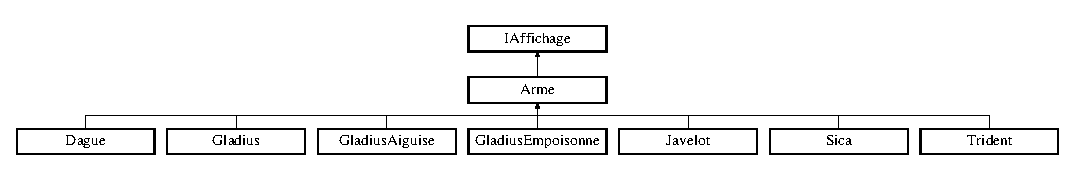
\includegraphics[height=1.846154cm]{class_arme}
\end{center}
\end{figure}
\subsection*{\-Public \-Member \-Functions}
\begin{DoxyCompactItemize}
\item 
int \hyperlink{class_arme_a6c957484697d9ad38ab1ed4361f3b8f4}{get\-Id} ()
\item 
void \hyperlink{class_arme_a332699f4c7b2dab9e38fccfddba7275b}{set\-Id} (int id)
\item 
string \hyperlink{class_arme_a5e43d33d0e14da19fb37dc497474135b}{get\-Libelle} ()
\item 
void \hyperlink{class_arme_ab38eebb032ab6773678ee40f152df6dd}{set\-Libelle} (string l)
\item 
virtual void \hyperlink{class_arme_ac815d060b7652e01e6813656d0880b20}{afficher\-Info} ()
\end{DoxyCompactItemize}


\subsection{\-Detailed \-Description}
\-Classe mère \hyperlink{class_arme}{\-Arme}, toutes les armes héritent de celle-\/ci \-Implémente l'interface \hyperlink{class_i_affichage}{\-I\-Affichage} 

\subsection{\-Member \-Function \-Documentation}
\hypertarget{class_arme_ac815d060b7652e01e6813656d0880b20}{\index{\-Arme@{\-Arme}!afficher\-Info@{afficher\-Info}}
\index{afficher\-Info@{afficher\-Info}!Arme@{\-Arme}}
\subsubsection[{afficher\-Info}]{\setlength{\rightskip}{0pt plus 5cm}virtual void {\bf \-Arme\-::afficher\-Info} (
\begin{DoxyParamCaption}
{}
\end{DoxyParamCaption}
)\hspace{0.3cm}{\ttfamily  \mbox{[}inline, virtual\mbox{]}}}}\label{class_arme_ac815d060b7652e01e6813656d0880b20}
\-Procédure d'affichage d'informations, redéfinit celle de l'interface \hyperlink{class_i_affichage}{\-I\-Affichage} 

\-Implements \hyperlink{class_i_affichage_a6123c1cb9079f712b48c0b8bf62e14ef}{\-I\-Affichage}.

\hypertarget{class_arme_a6c957484697d9ad38ab1ed4361f3b8f4}{\index{\-Arme@{\-Arme}!get\-Id@{get\-Id}}
\index{get\-Id@{get\-Id}!Arme@{\-Arme}}
\subsubsection[{get\-Id}]{\setlength{\rightskip}{0pt plus 5cm}int {\bf \-Arme\-::get\-Id} (
\begin{DoxyParamCaption}
{}
\end{DoxyParamCaption}
)\hspace{0.3cm}{\ttfamily  \mbox{[}inline\mbox{]}}}}\label{class_arme_a6c957484697d9ad38ab1ed4361f3b8f4}
\-Accesseur à l'identifiant de l'arme 

\-Reimplemented in \hyperlink{class_dague_afabd8cea0d60b3c8819c91005b395ca2}{\-Dague}, \hyperlink{class_gladius_a1eaed26d6372f759c570b77c2a623baf}{\-Gladius}, \hyperlink{class_javelot_aba1cccb47bf10d583936eae96284f49b}{\-Javelot}, \hyperlink{class_sica_a97460a3554bc4bc42b332fd0c267ee32}{\-Sica}, \hyperlink{class_trident_af6ffe8225c67ee4404cd0a571453a113}{\-Trident}, \hyperlink{class_gladius_aiguise_a9f54b9a3f9bc8bbb252dd9cc78d481d1}{\-Gladius\-Aiguise}, and \hyperlink{class_gladius_empoisonne_a23898d8572b5f9c552aec390cf474523}{\-Gladius\-Empoisonne}.

\hypertarget{class_arme_a5e43d33d0e14da19fb37dc497474135b}{\index{\-Arme@{\-Arme}!get\-Libelle@{get\-Libelle}}
\index{get\-Libelle@{get\-Libelle}!Arme@{\-Arme}}
\subsubsection[{get\-Libelle}]{\setlength{\rightskip}{0pt plus 5cm}string {\bf \-Arme\-::get\-Libelle} (
\begin{DoxyParamCaption}
{}
\end{DoxyParamCaption}
)\hspace{0.3cm}{\ttfamily  \mbox{[}inline\mbox{]}}}}\label{class_arme_a5e43d33d0e14da19fb37dc497474135b}
\-Accesseur au libellé de l'arme 

\-Reimplemented in \hyperlink{class_dague_a96e7b1ec98a4c8995223f58cb7d151b7}{\-Dague}, \hyperlink{class_gladius_ae303fc7e35a304fcc817ce220bf5e134}{\-Gladius}, \hyperlink{class_javelot_a37dca37b0f1756ad08352fe200fb6ed7}{\-Javelot}, \hyperlink{class_sica_ad7f3cf89e918b618c0ad76f40132e65e}{\-Sica}, \hyperlink{class_trident_a5a674900b64b6fb658828f99cbc222a5}{\-Trident}, \hyperlink{class_gladius_aiguise_afc73b6fd6b318112e11e6287fdbe9cff}{\-Gladius\-Aiguise}, and \hyperlink{class_gladius_empoisonne_a0db1471bda9bcd106c951ea5b1b9c7d5}{\-Gladius\-Empoisonne}.

\hypertarget{class_arme_a332699f4c7b2dab9e38fccfddba7275b}{\index{\-Arme@{\-Arme}!set\-Id@{set\-Id}}
\index{set\-Id@{set\-Id}!Arme@{\-Arme}}
\subsubsection[{set\-Id}]{\setlength{\rightskip}{0pt plus 5cm}void {\bf \-Arme\-::set\-Id} (
\begin{DoxyParamCaption}
\item[{int}]{id}
\end{DoxyParamCaption}
)\hspace{0.3cm}{\ttfamily  \mbox{[}inline\mbox{]}}}}\label{class_arme_a332699f4c7b2dab9e38fccfddba7275b}
\-Mutateur de l'identifiant de l'arme 

\-Reimplemented in \hyperlink{class_dague_a385f89995dd2e83f30891f2d356f8f48}{\-Dague}, \hyperlink{class_gladius_a73e8bacda8c1596704be5f165422d045}{\-Gladius}, \hyperlink{class_javelot_ab84399b82fc67e7ecf3c08081f24fec4}{\-Javelot}, \hyperlink{class_sica_a990b41f36bb50618e7911ebaa959c343}{\-Sica}, \hyperlink{class_trident_a3e64bc6cde8ae2e03875c7d256282de8}{\-Trident}, \hyperlink{class_gladius_aiguise_a32d93fce577bca09338829bcd8544674}{\-Gladius\-Aiguise}, and \hyperlink{class_gladius_empoisonne_ac2dba19740e6b5e4c20bd2b783499682}{\-Gladius\-Empoisonne}.

\hypertarget{class_arme_ab38eebb032ab6773678ee40f152df6dd}{\index{\-Arme@{\-Arme}!set\-Libelle@{set\-Libelle}}
\index{set\-Libelle@{set\-Libelle}!Arme@{\-Arme}}
\subsubsection[{set\-Libelle}]{\setlength{\rightskip}{0pt plus 5cm}void {\bf \-Arme\-::set\-Libelle} (
\begin{DoxyParamCaption}
\item[{string}]{l}
\end{DoxyParamCaption}
)\hspace{0.3cm}{\ttfamily  \mbox{[}inline\mbox{]}}}}\label{class_arme_ab38eebb032ab6773678ee40f152df6dd}
\-Mutateur du libellé de l'arme 

\-Reimplemented in \hyperlink{class_dague_af23c946232782f7d1e305317c2ce0444}{\-Dague}, \hyperlink{class_gladius_a42c4ac95a4bba0f81b7d7eabfef4dd40}{\-Gladius}, \hyperlink{class_javelot_a66872fd5e6d4a5704ec3c67264938f8e}{\-Javelot}, \hyperlink{class_sica_ab4ade5608a0321ef4fe1bc9b5ee85e17}{\-Sica}, \hyperlink{class_trident_ac9bc02a8c00777defffcc50cd8f42619}{\-Trident}, \hyperlink{class_gladius_aiguise_a36a9d4d8f0b92534ea50c1189be14d85}{\-Gladius\-Aiguise}, and \hyperlink{class_gladius_empoisonne_af7260cdfc296aecb4433ccf9a5b18dc7}{\-Gladius\-Empoisonne}.



\-The documentation for this class was generated from the following file\-:\begin{DoxyCompactItemize}
\item 
\-Projet\-P\-O\-O-\/master/\-Arme.\-cpp\end{DoxyCompactItemize}

\hypertarget{class_armure_legere}{\section{\-Armure\-Legere \-Class \-Reference}
\label{class_armure_legere}\index{\-Armure\-Legere@{\-Armure\-Legere}}
}
\-Inheritance diagram for \-Armure\-Legere\-:\begin{figure}[H]
\begin{center}
\leavevmode
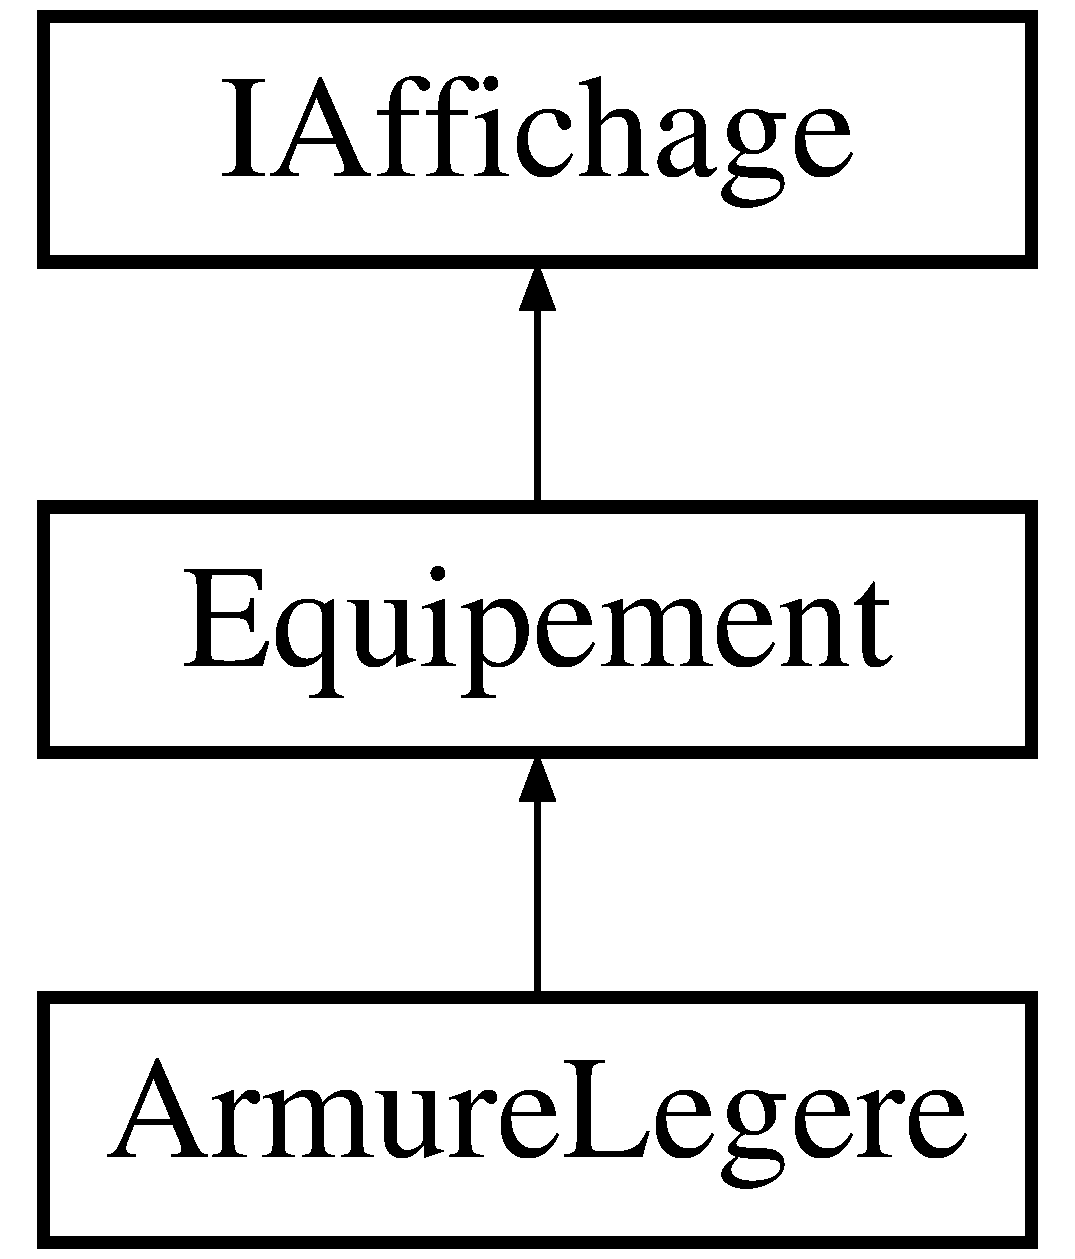
\includegraphics[height=3.000000cm]{class_armure_legere}
\end{center}
\end{figure}
\subsection*{\-Public \-Member \-Functions}
\begin{DoxyCompactItemize}
\item 
\hyperlink{class_armure_legere_ae074d68f3f168efb5f2bc479b848b89b}{\-Armure\-Legere} ()
\item 
int \hyperlink{class_armure_legere_a605de63de0fbb64f4170865ca8e7e851}{get\-Id} ()
\item 
void \hyperlink{class_armure_legere_a407cda69c45c312f8fa8df854504f717}{set\-Id} (int id)
\item 
string \hyperlink{class_armure_legere_a6201feeb0e1c65d756a2dc064a72b1c4}{get\-Libelle} ()
\item 
void \hyperlink{class_armure_legere_a403f2f2ad2300e361f50d29b5df7fda8}{set\-Libelle} (string l)
\item 
int \hyperlink{class_armure_legere_aa455d08100ac7895b1d1d7b61c92da3f}{get\-Val\-Def} ()
\item 
void \hyperlink{class_armure_legere_a827399af549f7fd182c9ff96be61a4d0}{set\-Val\-Def} (int v)
\end{DoxyCompactItemize}


\subsection{\-Detailed \-Description}
\-Classe \hyperlink{class_armure_legere}{\-Armure\-Legere}, hérite d'\hyperlink{class_equipement}{\-Equipement} 

\subsection{\-Constructor \& \-Destructor \-Documentation}
\hypertarget{class_armure_legere_ae074d68f3f168efb5f2bc479b848b89b}{\index{\-Armure\-Legere@{\-Armure\-Legere}!\-Armure\-Legere@{\-Armure\-Legere}}
\index{\-Armure\-Legere@{\-Armure\-Legere}!ArmureLegere@{\-Armure\-Legere}}
\subsubsection[{\-Armure\-Legere}]{\setlength{\rightskip}{0pt plus 5cm}{\bf \-Armure\-Legere\-::\-Armure\-Legere} (
\begin{DoxyParamCaption}
{}
\end{DoxyParamCaption}
)\hspace{0.3cm}{\ttfamily  \mbox{[}inline\mbox{]}}}}\label{class_armure_legere_ae074d68f3f168efb5f2bc479b848b89b}
\-Constructeur explicite initialisant les variables de l'armure 

\subsection{\-Member \-Function \-Documentation}
\hypertarget{class_armure_legere_a605de63de0fbb64f4170865ca8e7e851}{\index{\-Armure\-Legere@{\-Armure\-Legere}!get\-Id@{get\-Id}}
\index{get\-Id@{get\-Id}!ArmureLegere@{\-Armure\-Legere}}
\subsubsection[{get\-Id}]{\setlength{\rightskip}{0pt plus 5cm}int {\bf \-Armure\-Legere\-::get\-Id} (
\begin{DoxyParamCaption}
{}
\end{DoxyParamCaption}
)\hspace{0.3cm}{\ttfamily  \mbox{[}inline\mbox{]}}}}\label{class_armure_legere_a605de63de0fbb64f4170865ca8e7e851}
\-Accesseur à l'identifiant de l'armure 

\-Reimplemented from \hyperlink{class_equipement_abc38941f5a9deed943b7a83ce69539c3}{\-Equipement}.

\hypertarget{class_armure_legere_a6201feeb0e1c65d756a2dc064a72b1c4}{\index{\-Armure\-Legere@{\-Armure\-Legere}!get\-Libelle@{get\-Libelle}}
\index{get\-Libelle@{get\-Libelle}!ArmureLegere@{\-Armure\-Legere}}
\subsubsection[{get\-Libelle}]{\setlength{\rightskip}{0pt plus 5cm}string {\bf \-Armure\-Legere\-::get\-Libelle} (
\begin{DoxyParamCaption}
{}
\end{DoxyParamCaption}
)\hspace{0.3cm}{\ttfamily  \mbox{[}inline\mbox{]}}}}\label{class_armure_legere_a6201feeb0e1c65d756a2dc064a72b1c4}
\-Accesseur au libellé de l'équipement 

\-Reimplemented from \hyperlink{class_equipement_ab00ec565966647bf6edeb1a9df430aa6}{\-Equipement}.

\hypertarget{class_armure_legere_aa455d08100ac7895b1d1d7b61c92da3f}{\index{\-Armure\-Legere@{\-Armure\-Legere}!get\-Val\-Def@{get\-Val\-Def}}
\index{get\-Val\-Def@{get\-Val\-Def}!ArmureLegere@{\-Armure\-Legere}}
\subsubsection[{get\-Val\-Def}]{\setlength{\rightskip}{0pt plus 5cm}int {\bf \-Armure\-Legere\-::get\-Val\-Def} (
\begin{DoxyParamCaption}
{}
\end{DoxyParamCaption}
)\hspace{0.3cm}{\ttfamily  \mbox{[}inline\mbox{]}}}}\label{class_armure_legere_aa455d08100ac7895b1d1d7b61c92da3f}
\-Accesseur à la valeur de défense de l'armure 

\-Reimplemented from \hyperlink{class_equipement_a7b3003f4da24a94bfec94555e35e772c}{\-Equipement}.

\hypertarget{class_armure_legere_a407cda69c45c312f8fa8df854504f717}{\index{\-Armure\-Legere@{\-Armure\-Legere}!set\-Id@{set\-Id}}
\index{set\-Id@{set\-Id}!ArmureLegere@{\-Armure\-Legere}}
\subsubsection[{set\-Id}]{\setlength{\rightskip}{0pt plus 5cm}void {\bf \-Armure\-Legere\-::set\-Id} (
\begin{DoxyParamCaption}
\item[{int}]{id}
\end{DoxyParamCaption}
)\hspace{0.3cm}{\ttfamily  \mbox{[}inline\mbox{]}}}}\label{class_armure_legere_a407cda69c45c312f8fa8df854504f717}
\-Mutateur de l'identifiant de l'armure 

\-Reimplemented from \hyperlink{class_equipement_a98208826ad05cbc38211e9f70bd908c5}{\-Equipement}.

\hypertarget{class_armure_legere_a403f2f2ad2300e361f50d29b5df7fda8}{\index{\-Armure\-Legere@{\-Armure\-Legere}!set\-Libelle@{set\-Libelle}}
\index{set\-Libelle@{set\-Libelle}!ArmureLegere@{\-Armure\-Legere}}
\subsubsection[{set\-Libelle}]{\setlength{\rightskip}{0pt plus 5cm}void {\bf \-Armure\-Legere\-::set\-Libelle} (
\begin{DoxyParamCaption}
\item[{string}]{l}
\end{DoxyParamCaption}
)\hspace{0.3cm}{\ttfamily  \mbox{[}inline\mbox{]}}}}\label{class_armure_legere_a403f2f2ad2300e361f50d29b5df7fda8}
\-Mutateur du libellé de l'équipement 

\-Reimplemented from \hyperlink{class_equipement_aea246b68c747bd5ec84ca8ce4c4c7b40}{\-Equipement}.

\hypertarget{class_armure_legere_a827399af549f7fd182c9ff96be61a4d0}{\index{\-Armure\-Legere@{\-Armure\-Legere}!set\-Val\-Def@{set\-Val\-Def}}
\index{set\-Val\-Def@{set\-Val\-Def}!ArmureLegere@{\-Armure\-Legere}}
\subsubsection[{set\-Val\-Def}]{\setlength{\rightskip}{0pt plus 5cm}void {\bf \-Armure\-Legere\-::set\-Val\-Def} (
\begin{DoxyParamCaption}
\item[{int}]{v}
\end{DoxyParamCaption}
)\hspace{0.3cm}{\ttfamily  \mbox{[}inline\mbox{]}}}}\label{class_armure_legere_a827399af549f7fd182c9ff96be61a4d0}
\-Mutateur de la valeur de défense de l'armure 

\-Reimplemented from \hyperlink{class_equipement_ad9940c901b3a96b91c5c3f24713face5}{\-Equipement}.



\-The documentation for this class was generated from the following file\-:\begin{DoxyCompactItemize}
\item 
\-Projet\-P\-O\-O-\/master/\-Armure\-Legere.\-cpp\end{DoxyCompactItemize}

\hypertarget{class_bras_droit}{\section{\-Bras\-Droit \-Class \-Reference}
\label{class_bras_droit}\index{\-Bras\-Droit@{\-Bras\-Droit}}
}
\-Inheritance diagram for \-Bras\-Droit\-:\begin{figure}[H]
\begin{center}
\leavevmode
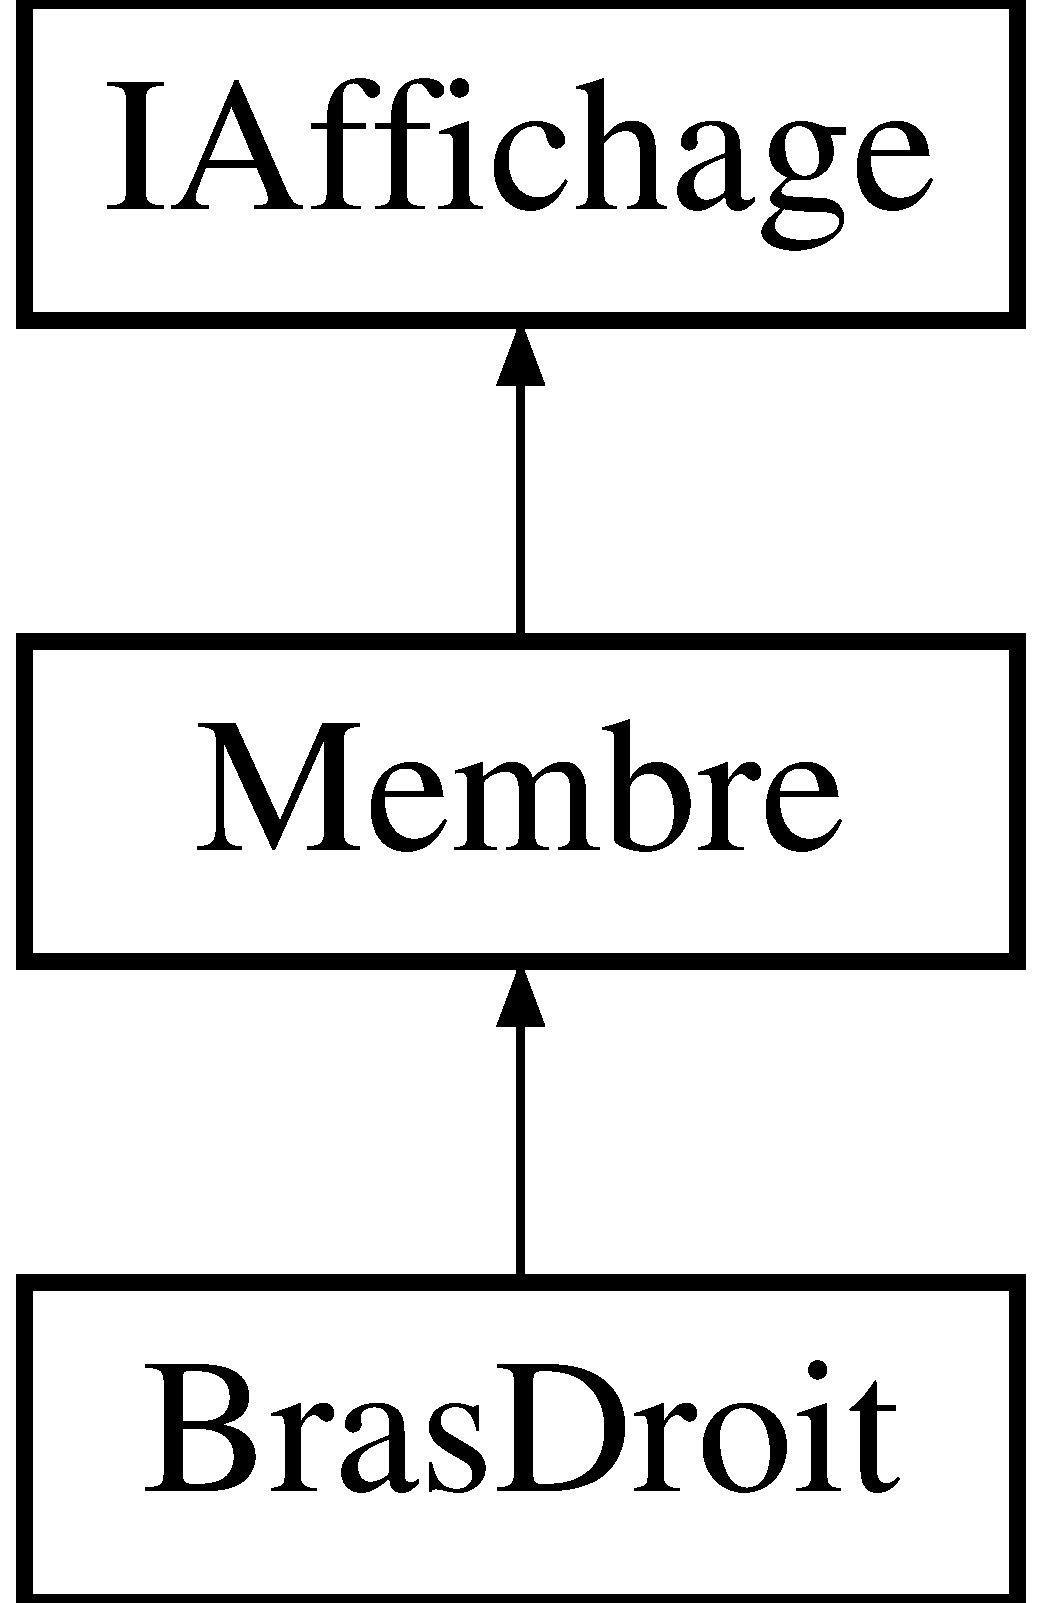
\includegraphics[height=3.000000cm]{class_bras_droit}
\end{center}
\end{figure}
\subsection*{\-Public \-Member \-Functions}
\begin{DoxyCompactItemize}
\item 
\hyperlink{class_bras_droit_a5478c047502eac41e3c300dccb8bb3d1}{\-Bras\-Droit} ()
\item 
int \hyperlink{class_bras_droit_a9be3f4a94a82e95caa78aaabc6357c2b}{get\-Id} ()
\item 
void \hyperlink{class_bras_droit_a156189452ba3e3d037ecca9b21d294cb}{set\-Id} (int id)
\item 
int \hyperlink{class_bras_droit_adddfb977411421906d39f4bd4a35daf1}{get\-P\-D\-V} ()
\item 
void \hyperlink{class_bras_droit_a519053f32bea237a7fe8f7c93d9a0152}{set\-P\-D\-V} (int p)
\item 
string \hyperlink{class_bras_droit_a6db96c33ab1043b39127277d1920a63f}{get\-Libelle} ()
\item 
void \hyperlink{class_bras_droit_adc1f6283b4e00813a099b5cc9b9f8d76}{set\-Libelle} (string l)
\item 
\hyperlink{class_equipement}{\-Equipement} \hyperlink{class_bras_droit_a9af72d2589c8c33cc5e5d5e666424957}{get\-Equip} ()
\item 
\hyperlink{class_equipement}{\-Equipement} \hyperlink{class_bras_droit_a726fd8be859bbb27257118ad4c3647dc}{set\-Equip} (\hyperlink{class_equipement}{\-Equipement} e)
\end{DoxyCompactItemize}


\subsection{\-Detailed \-Description}
\-Classe \hyperlink{class_bras_droit}{\-Bras\-Droit}, hérite de \hyperlink{class_membre}{\-Membre} 

\subsection{\-Constructor \& \-Destructor \-Documentation}
\hypertarget{class_bras_droit_a5478c047502eac41e3c300dccb8bb3d1}{\index{\-Bras\-Droit@{\-Bras\-Droit}!\-Bras\-Droit@{\-Bras\-Droit}}
\index{\-Bras\-Droit@{\-Bras\-Droit}!BrasDroit@{\-Bras\-Droit}}
\subsubsection[{\-Bras\-Droit}]{\setlength{\rightskip}{0pt plus 5cm}{\bf \-Bras\-Droit\-::\-Bras\-Droit} (
\begin{DoxyParamCaption}
{}
\end{DoxyParamCaption}
)\hspace{0.3cm}{\ttfamily  \mbox{[}inline\mbox{]}}}}\label{class_bras_droit_a5478c047502eac41e3c300dccb8bb3d1}
\-Constructeur explicite initialisant les variables du bras droit 

\subsection{\-Member \-Function \-Documentation}
\hypertarget{class_bras_droit_a9af72d2589c8c33cc5e5d5e666424957}{\index{\-Bras\-Droit@{\-Bras\-Droit}!get\-Equip@{get\-Equip}}
\index{get\-Equip@{get\-Equip}!BrasDroit@{\-Bras\-Droit}}
\subsubsection[{get\-Equip}]{\setlength{\rightskip}{0pt plus 5cm}{\bf \-Equipement} {\bf \-Bras\-Droit\-::get\-Equip} (
\begin{DoxyParamCaption}
{}
\end{DoxyParamCaption}
)\hspace{0.3cm}{\ttfamily  \mbox{[}inline\mbox{]}}}}\label{class_bras_droit_a9af72d2589c8c33cc5e5d5e666424957}
\-Accesseur à l'\hyperlink{class_equipement}{\-Equipement} équipé au bras droit 

\-Reimplemented from \hyperlink{class_membre_a8b57b95b91806ebf6171624ac0a051cb}{\-Membre}.

\hypertarget{class_bras_droit_a9be3f4a94a82e95caa78aaabc6357c2b}{\index{\-Bras\-Droit@{\-Bras\-Droit}!get\-Id@{get\-Id}}
\index{get\-Id@{get\-Id}!BrasDroit@{\-Bras\-Droit}}
\subsubsection[{get\-Id}]{\setlength{\rightskip}{0pt plus 5cm}int {\bf \-Bras\-Droit\-::get\-Id} (
\begin{DoxyParamCaption}
{}
\end{DoxyParamCaption}
)\hspace{0.3cm}{\ttfamily  \mbox{[}inline\mbox{]}}}}\label{class_bras_droit_a9be3f4a94a82e95caa78aaabc6357c2b}
\-Accesseur à l'identifiant du bras droit 

\-Reimplemented from \hyperlink{class_membre_aa4ba3c5babf132246cc84907c37e3738}{\-Membre}.

\hypertarget{class_bras_droit_a6db96c33ab1043b39127277d1920a63f}{\index{\-Bras\-Droit@{\-Bras\-Droit}!get\-Libelle@{get\-Libelle}}
\index{get\-Libelle@{get\-Libelle}!BrasDroit@{\-Bras\-Droit}}
\subsubsection[{get\-Libelle}]{\setlength{\rightskip}{0pt plus 5cm}string {\bf \-Bras\-Droit\-::get\-Libelle} (
\begin{DoxyParamCaption}
{}
\end{DoxyParamCaption}
)\hspace{0.3cm}{\ttfamily  \mbox{[}inline\mbox{]}}}}\label{class_bras_droit_a6db96c33ab1043b39127277d1920a63f}
\-Accesseur au libellé du membre 

\-Reimplemented from \hyperlink{class_membre_a6ef6931754fe7ce7e8101bf27bc3ef6a}{\-Membre}.

\hypertarget{class_bras_droit_adddfb977411421906d39f4bd4a35daf1}{\index{\-Bras\-Droit@{\-Bras\-Droit}!get\-P\-D\-V@{get\-P\-D\-V}}
\index{get\-P\-D\-V@{get\-P\-D\-V}!BrasDroit@{\-Bras\-Droit}}
\subsubsection[{get\-P\-D\-V}]{\setlength{\rightskip}{0pt plus 5cm}int {\bf \-Bras\-Droit\-::get\-P\-D\-V} (
\begin{DoxyParamCaption}
{}
\end{DoxyParamCaption}
)\hspace{0.3cm}{\ttfamily  \mbox{[}inline\mbox{]}}}}\label{class_bras_droit_adddfb977411421906d39f4bd4a35daf1}
\-Accesseur au nombre de points de vie du bras droit 

\-Reimplemented from \hyperlink{class_membre_a35ddd831b2ca01dd13be213470f2aa65}{\-Membre}.

\hypertarget{class_bras_droit_a726fd8be859bbb27257118ad4c3647dc}{\index{\-Bras\-Droit@{\-Bras\-Droit}!set\-Equip@{set\-Equip}}
\index{set\-Equip@{set\-Equip}!BrasDroit@{\-Bras\-Droit}}
\subsubsection[{set\-Equip}]{\setlength{\rightskip}{0pt plus 5cm}{\bf \-Equipement} {\bf \-Bras\-Droit\-::set\-Equip} (
\begin{DoxyParamCaption}
\item[{{\bf \-Equipement}}]{e}
\end{DoxyParamCaption}
)\hspace{0.3cm}{\ttfamily  \mbox{[}inline\mbox{]}}}}\label{class_bras_droit_a726fd8be859bbb27257118ad4c3647dc}
\-Mutateur de l'\hyperlink{class_equipement}{\-Equipement} équipé au bras droit 

\-Reimplemented from \hyperlink{class_membre_ab2f78da0480458242168b57cf33e3f7c}{\-Membre}.

\hypertarget{class_bras_droit_a156189452ba3e3d037ecca9b21d294cb}{\index{\-Bras\-Droit@{\-Bras\-Droit}!set\-Id@{set\-Id}}
\index{set\-Id@{set\-Id}!BrasDroit@{\-Bras\-Droit}}
\subsubsection[{set\-Id}]{\setlength{\rightskip}{0pt plus 5cm}void {\bf \-Bras\-Droit\-::set\-Id} (
\begin{DoxyParamCaption}
\item[{int}]{id}
\end{DoxyParamCaption}
)\hspace{0.3cm}{\ttfamily  \mbox{[}inline\mbox{]}}}}\label{class_bras_droit_a156189452ba3e3d037ecca9b21d294cb}
\-Mutateur de l'identifiant du bras droit 

\-Reimplemented from \hyperlink{class_membre_a4b87bebc56e82f08d4ebdf8bcf773c11}{\-Membre}.

\hypertarget{class_bras_droit_adc1f6283b4e00813a099b5cc9b9f8d76}{\index{\-Bras\-Droit@{\-Bras\-Droit}!set\-Libelle@{set\-Libelle}}
\index{set\-Libelle@{set\-Libelle}!BrasDroit@{\-Bras\-Droit}}
\subsubsection[{set\-Libelle}]{\setlength{\rightskip}{0pt plus 5cm}void {\bf \-Bras\-Droit\-::set\-Libelle} (
\begin{DoxyParamCaption}
\item[{string}]{l}
\end{DoxyParamCaption}
)\hspace{0.3cm}{\ttfamily  \mbox{[}inline\mbox{]}}}}\label{class_bras_droit_adc1f6283b4e00813a099b5cc9b9f8d76}
\-Mutateur du libellé du membre 

\-Reimplemented from \hyperlink{class_membre_aaffef4990f332871cd1dd9b3fc03a078}{\-Membre}.

\hypertarget{class_bras_droit_a519053f32bea237a7fe8f7c93d9a0152}{\index{\-Bras\-Droit@{\-Bras\-Droit}!set\-P\-D\-V@{set\-P\-D\-V}}
\index{set\-P\-D\-V@{set\-P\-D\-V}!BrasDroit@{\-Bras\-Droit}}
\subsubsection[{set\-P\-D\-V}]{\setlength{\rightskip}{0pt plus 5cm}void {\bf \-Bras\-Droit\-::set\-P\-D\-V} (
\begin{DoxyParamCaption}
\item[{int}]{p}
\end{DoxyParamCaption}
)\hspace{0.3cm}{\ttfamily  \mbox{[}inline\mbox{]}}}}\label{class_bras_droit_a519053f32bea237a7fe8f7c93d9a0152}
\-Mutateur du nombre de points de vie du bras droit 

\-Reimplemented from \hyperlink{class_membre_a6b45657cd705c02a6ab5a338d1204f3e}{\-Membre}.



\-The documentation for this class was generated from the following file\-:\begin{DoxyCompactItemize}
\item 
\-Projet\-P\-O\-O-\/master/\-Bras\-Droit.\-cpp\end{DoxyCompactItemize}

\hypertarget{class_bras_gauche}{\section{\-Bras\-Gauche \-Class \-Reference}
\label{class_bras_gauche}\index{\-Bras\-Gauche@{\-Bras\-Gauche}}
}
\-Inheritance diagram for \-Bras\-Gauche\-:\begin{figure}[H]
\begin{center}
\leavevmode
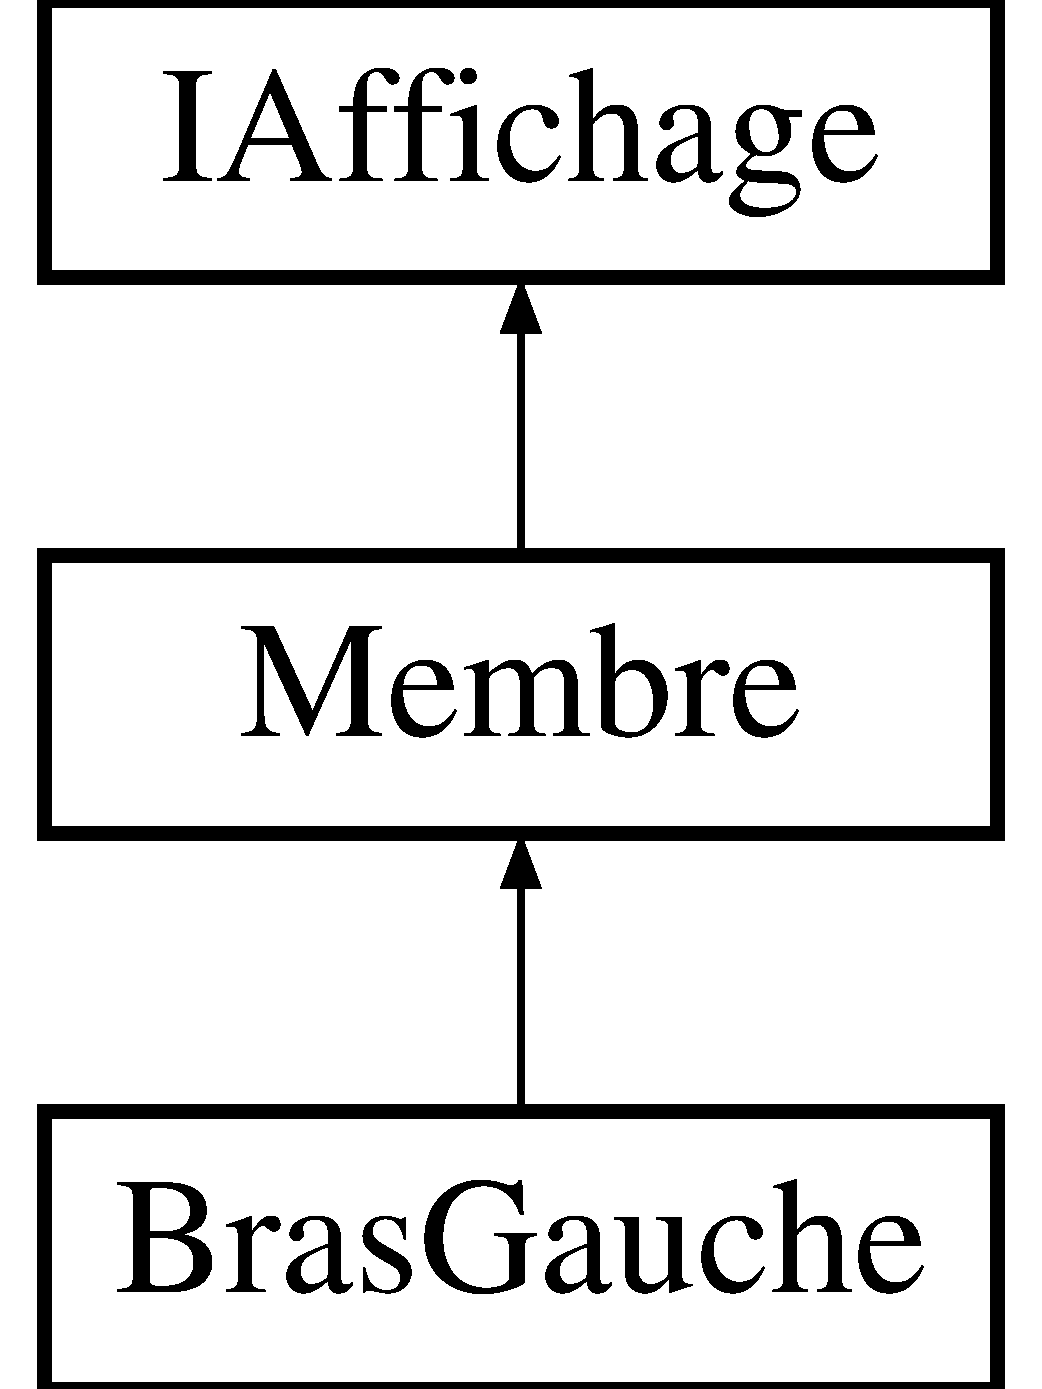
\includegraphics[height=3.000000cm]{class_bras_gauche}
\end{center}
\end{figure}
\subsection*{\-Public \-Member \-Functions}
\begin{DoxyCompactItemize}
\item 
\hyperlink{class_bras_gauche_a853b7a5ea4ad2126c031e5997b2066e0}{\-Bras\-Gauche} ()
\item 
int \hyperlink{class_bras_gauche_ad30956e6d1afe81c57ed5545bfe7b0e6}{get\-Id} ()
\item 
void \hyperlink{class_bras_gauche_a0e1accaf25773a48d64f716a6389c33c}{set\-Id} (int id)
\item 
int \hyperlink{class_bras_gauche_a24954e20008bc8724156731b5450b91f}{get\-P\-D\-V} ()
\item 
void \hyperlink{class_bras_gauche_ac5698d46c3af46fcaaf9a6cd5cd3d495}{set\-P\-D\-V} (int p)
\item 
string \hyperlink{class_bras_gauche_a0c22b277eae6cf0a0475f02f5037db1f}{get\-Libelle} ()
\item 
void \hyperlink{class_bras_gauche_a64e26bbb9af48a13f9c4b128ddb74570}{set\-Libelle} (string l)
\item 
\hyperlink{class_equipement}{\-Equipement} \hyperlink{class_bras_gauche_abc90f6e5e9d8fb71f5b7c76cc51d8e48}{get\-Equip} ()
\item 
\hyperlink{class_equipement}{\-Equipement} \hyperlink{class_bras_gauche_ad99fefc88e948e61c781a76b4262102b}{set\-Equip} (\hyperlink{class_equipement}{\-Equipement} e)
\end{DoxyCompactItemize}


\subsection{\-Detailed \-Description}
\-Classe \hyperlink{class_bras_gauche}{\-Bras\-Gauche}, hérite de \hyperlink{class_membre}{\-Membre} 

\subsection{\-Constructor \& \-Destructor \-Documentation}
\hypertarget{class_bras_gauche_a853b7a5ea4ad2126c031e5997b2066e0}{\index{\-Bras\-Gauche@{\-Bras\-Gauche}!\-Bras\-Gauche@{\-Bras\-Gauche}}
\index{\-Bras\-Gauche@{\-Bras\-Gauche}!BrasGauche@{\-Bras\-Gauche}}
\subsubsection[{\-Bras\-Gauche}]{\setlength{\rightskip}{0pt plus 5cm}{\bf \-Bras\-Gauche\-::\-Bras\-Gauche} (
\begin{DoxyParamCaption}
{}
\end{DoxyParamCaption}
)\hspace{0.3cm}{\ttfamily  \mbox{[}inline\mbox{]}}}}\label{class_bras_gauche_a853b7a5ea4ad2126c031e5997b2066e0}
\-Constructeur explicite initialisant les variables du bras gauche 

\subsection{\-Member \-Function \-Documentation}
\hypertarget{class_bras_gauche_abc90f6e5e9d8fb71f5b7c76cc51d8e48}{\index{\-Bras\-Gauche@{\-Bras\-Gauche}!get\-Equip@{get\-Equip}}
\index{get\-Equip@{get\-Equip}!BrasGauche@{\-Bras\-Gauche}}
\subsubsection[{get\-Equip}]{\setlength{\rightskip}{0pt plus 5cm}{\bf \-Equipement} {\bf \-Bras\-Gauche\-::get\-Equip} (
\begin{DoxyParamCaption}
{}
\end{DoxyParamCaption}
)\hspace{0.3cm}{\ttfamily  \mbox{[}inline\mbox{]}}}}\label{class_bras_gauche_abc90f6e5e9d8fb71f5b7c76cc51d8e48}
\-Accesseur à l'\hyperlink{class_equipement}{\-Equipement} équipé au bras gauche 

\-Reimplemented from \hyperlink{class_membre_a8b57b95b91806ebf6171624ac0a051cb}{\-Membre}.

\hypertarget{class_bras_gauche_ad30956e6d1afe81c57ed5545bfe7b0e6}{\index{\-Bras\-Gauche@{\-Bras\-Gauche}!get\-Id@{get\-Id}}
\index{get\-Id@{get\-Id}!BrasGauche@{\-Bras\-Gauche}}
\subsubsection[{get\-Id}]{\setlength{\rightskip}{0pt plus 5cm}int {\bf \-Bras\-Gauche\-::get\-Id} (
\begin{DoxyParamCaption}
{}
\end{DoxyParamCaption}
)\hspace{0.3cm}{\ttfamily  \mbox{[}inline\mbox{]}}}}\label{class_bras_gauche_ad30956e6d1afe81c57ed5545bfe7b0e6}
\-Accesseur à l'identifiant du bras gauche 

\-Reimplemented from \hyperlink{class_membre_aa4ba3c5babf132246cc84907c37e3738}{\-Membre}.

\hypertarget{class_bras_gauche_a0c22b277eae6cf0a0475f02f5037db1f}{\index{\-Bras\-Gauche@{\-Bras\-Gauche}!get\-Libelle@{get\-Libelle}}
\index{get\-Libelle@{get\-Libelle}!BrasGauche@{\-Bras\-Gauche}}
\subsubsection[{get\-Libelle}]{\setlength{\rightskip}{0pt plus 5cm}string {\bf \-Bras\-Gauche\-::get\-Libelle} (
\begin{DoxyParamCaption}
{}
\end{DoxyParamCaption}
)\hspace{0.3cm}{\ttfamily  \mbox{[}inline\mbox{]}}}}\label{class_bras_gauche_a0c22b277eae6cf0a0475f02f5037db1f}
\-Accesseur au libellé du membre 

\-Reimplemented from \hyperlink{class_membre_a6ef6931754fe7ce7e8101bf27bc3ef6a}{\-Membre}.

\hypertarget{class_bras_gauche_a24954e20008bc8724156731b5450b91f}{\index{\-Bras\-Gauche@{\-Bras\-Gauche}!get\-P\-D\-V@{get\-P\-D\-V}}
\index{get\-P\-D\-V@{get\-P\-D\-V}!BrasGauche@{\-Bras\-Gauche}}
\subsubsection[{get\-P\-D\-V}]{\setlength{\rightskip}{0pt plus 5cm}int {\bf \-Bras\-Gauche\-::get\-P\-D\-V} (
\begin{DoxyParamCaption}
{}
\end{DoxyParamCaption}
)\hspace{0.3cm}{\ttfamily  \mbox{[}inline\mbox{]}}}}\label{class_bras_gauche_a24954e20008bc8724156731b5450b91f}
\-Accesseur au nombre de points de vie du bras gauche 

\-Reimplemented from \hyperlink{class_membre_a35ddd831b2ca01dd13be213470f2aa65}{\-Membre}.

\hypertarget{class_bras_gauche_ad99fefc88e948e61c781a76b4262102b}{\index{\-Bras\-Gauche@{\-Bras\-Gauche}!set\-Equip@{set\-Equip}}
\index{set\-Equip@{set\-Equip}!BrasGauche@{\-Bras\-Gauche}}
\subsubsection[{set\-Equip}]{\setlength{\rightskip}{0pt plus 5cm}{\bf \-Equipement} {\bf \-Bras\-Gauche\-::set\-Equip} (
\begin{DoxyParamCaption}
\item[{{\bf \-Equipement}}]{e}
\end{DoxyParamCaption}
)\hspace{0.3cm}{\ttfamily  \mbox{[}inline\mbox{]}}}}\label{class_bras_gauche_ad99fefc88e948e61c781a76b4262102b}
\-Mutateur de l'\hyperlink{class_equipement}{\-Equipement} équipé au bras gauche 

\-Reimplemented from \hyperlink{class_membre_ab2f78da0480458242168b57cf33e3f7c}{\-Membre}.

\hypertarget{class_bras_gauche_a0e1accaf25773a48d64f716a6389c33c}{\index{\-Bras\-Gauche@{\-Bras\-Gauche}!set\-Id@{set\-Id}}
\index{set\-Id@{set\-Id}!BrasGauche@{\-Bras\-Gauche}}
\subsubsection[{set\-Id}]{\setlength{\rightskip}{0pt plus 5cm}void {\bf \-Bras\-Gauche\-::set\-Id} (
\begin{DoxyParamCaption}
\item[{int}]{id}
\end{DoxyParamCaption}
)\hspace{0.3cm}{\ttfamily  \mbox{[}inline\mbox{]}}}}\label{class_bras_gauche_a0e1accaf25773a48d64f716a6389c33c}
\-Mutateur de l'identifiant du bras gauche 

\-Reimplemented from \hyperlink{class_membre_a4b87bebc56e82f08d4ebdf8bcf773c11}{\-Membre}.

\hypertarget{class_bras_gauche_a64e26bbb9af48a13f9c4b128ddb74570}{\index{\-Bras\-Gauche@{\-Bras\-Gauche}!set\-Libelle@{set\-Libelle}}
\index{set\-Libelle@{set\-Libelle}!BrasGauche@{\-Bras\-Gauche}}
\subsubsection[{set\-Libelle}]{\setlength{\rightskip}{0pt plus 5cm}void {\bf \-Bras\-Gauche\-::set\-Libelle} (
\begin{DoxyParamCaption}
\item[{string}]{l}
\end{DoxyParamCaption}
)\hspace{0.3cm}{\ttfamily  \mbox{[}inline\mbox{]}}}}\label{class_bras_gauche_a64e26bbb9af48a13f9c4b128ddb74570}
\-Mutateur du libellé du membre 

\-Reimplemented from \hyperlink{class_membre_aaffef4990f332871cd1dd9b3fc03a078}{\-Membre}.

\hypertarget{class_bras_gauche_ac5698d46c3af46fcaaf9a6cd5cd3d495}{\index{\-Bras\-Gauche@{\-Bras\-Gauche}!set\-P\-D\-V@{set\-P\-D\-V}}
\index{set\-P\-D\-V@{set\-P\-D\-V}!BrasGauche@{\-Bras\-Gauche}}
\subsubsection[{set\-P\-D\-V}]{\setlength{\rightskip}{0pt plus 5cm}void {\bf \-Bras\-Gauche\-::set\-P\-D\-V} (
\begin{DoxyParamCaption}
\item[{int}]{p}
\end{DoxyParamCaption}
)\hspace{0.3cm}{\ttfamily  \mbox{[}inline\mbox{]}}}}\label{class_bras_gauche_ac5698d46c3af46fcaaf9a6cd5cd3d495}
\-Mutateur du nombre de points de vie du bras gauche 

\-Reimplemented from \hyperlink{class_membre_a6b45657cd705c02a6ab5a338d1204f3e}{\-Membre}.



\-The documentation for this class was generated from the following file\-:\begin{DoxyCompactItemize}
\item 
\-Projet\-P\-O\-O-\/master/\-Bras\-Gauche.\-cpp\end{DoxyCompactItemize}

\hypertarget{class_casque}{\section{\-Casque \-Class \-Reference}
\label{class_casque}\index{\-Casque@{\-Casque}}
}
\-Inheritance diagram for \-Casque\-:\begin{figure}[H]
\begin{center}
\leavevmode
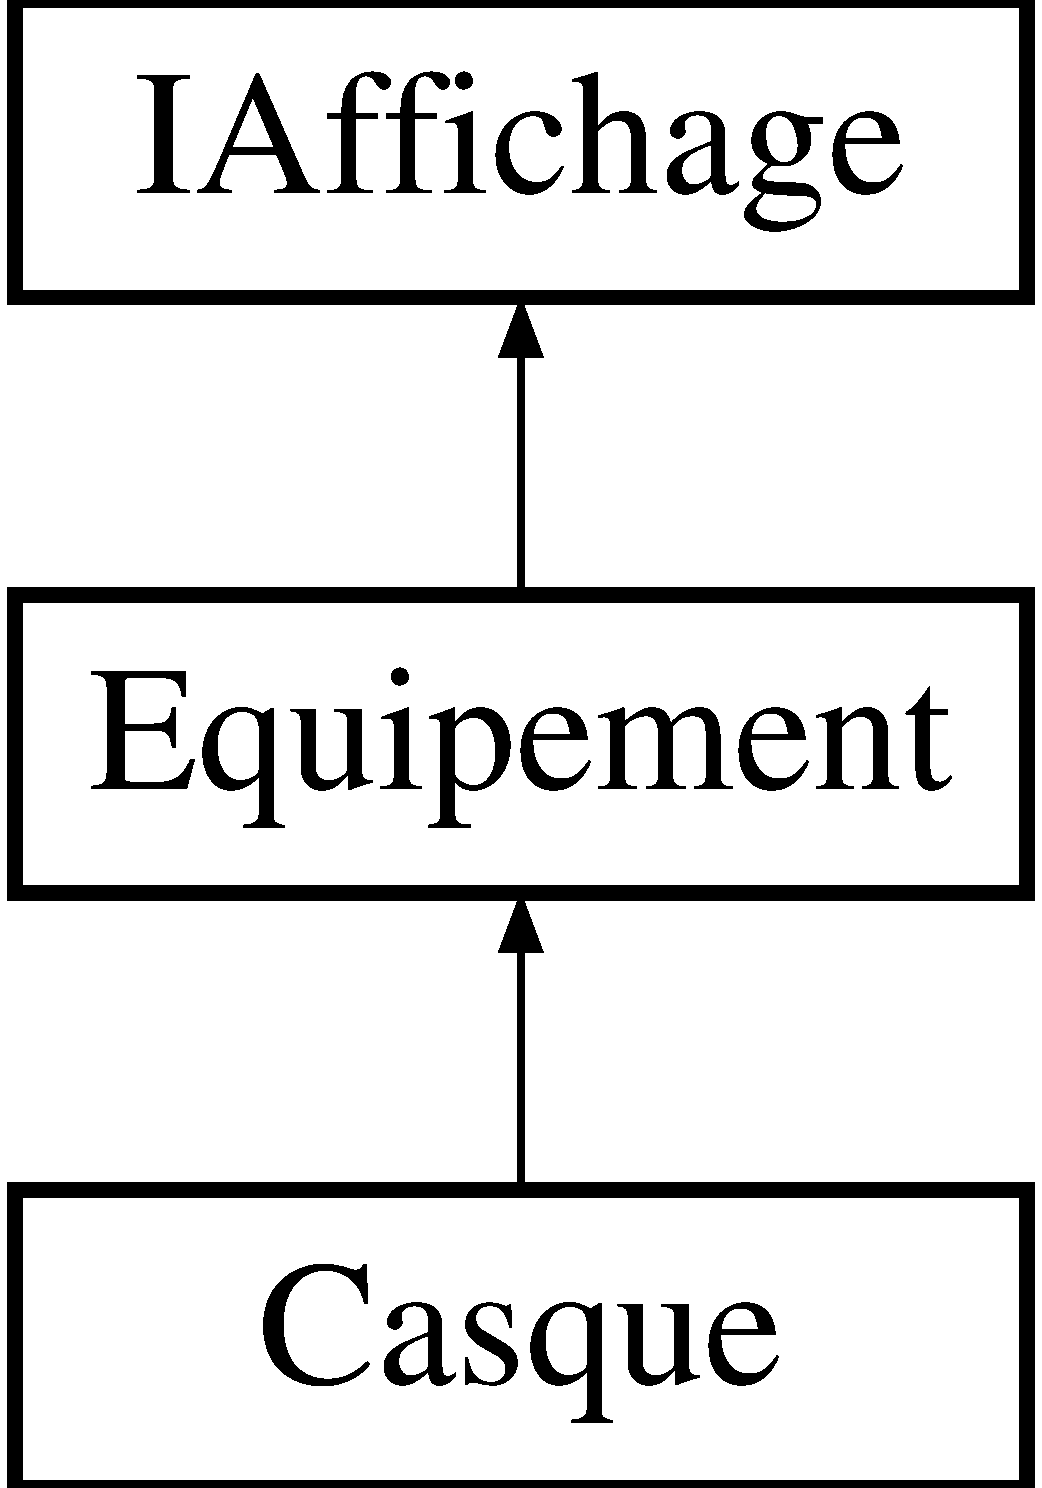
\includegraphics[height=3.000000cm]{class_casque}
\end{center}
\end{figure}
\subsection*{\-Public \-Member \-Functions}
\begin{DoxyCompactItemize}
\item 
\hyperlink{class_casque_af3f27280f4291d04f16157c7e03ec625}{\-Casque} ()
\item 
int \hyperlink{class_casque_a274f8d36daf144145d716bb4f09d92ae}{get\-Id} ()
\item 
void \hyperlink{class_casque_aa6c352baa2c050aaa0b525fbe260a7c9}{set\-Id} (int id)
\item 
string \hyperlink{class_casque_a408f8a20ef9a6513e3798975926c329b}{get\-Libelle} ()
\item 
void \hyperlink{class_casque_a3a9bdab95f79ca64e5c49b81f0ff1295}{set\-Libelle} (string l)
\item 
int \hyperlink{class_casque_a899bc40890f9afaccc665bc816864084}{get\-Val\-Def} ()
\item 
void \hyperlink{class_casque_a7d4eee2cf255fbbac8d308560e572c57}{set\-Val\-Def} (int v)
\end{DoxyCompactItemize}


\subsection{\-Detailed \-Description}
\-Classe \hyperlink{class_casque}{\-Casque}, hérite d'\hyperlink{class_equipement}{\-Equipement} 

\subsection{\-Constructor \& \-Destructor \-Documentation}
\hypertarget{class_casque_af3f27280f4291d04f16157c7e03ec625}{\index{\-Casque@{\-Casque}!\-Casque@{\-Casque}}
\index{\-Casque@{\-Casque}!Casque@{\-Casque}}
\subsubsection[{\-Casque}]{\setlength{\rightskip}{0pt plus 5cm}{\bf \-Casque\-::\-Casque} (
\begin{DoxyParamCaption}
{}
\end{DoxyParamCaption}
)\hspace{0.3cm}{\ttfamily  \mbox{[}inline\mbox{]}}}}\label{class_casque_af3f27280f4291d04f16157c7e03ec625}
\-Constructeur explicite initialisant les valeurs du casque 

\subsection{\-Member \-Function \-Documentation}
\hypertarget{class_casque_a274f8d36daf144145d716bb4f09d92ae}{\index{\-Casque@{\-Casque}!get\-Id@{get\-Id}}
\index{get\-Id@{get\-Id}!Casque@{\-Casque}}
\subsubsection[{get\-Id}]{\setlength{\rightskip}{0pt plus 5cm}int {\bf \-Casque\-::get\-Id} (
\begin{DoxyParamCaption}
{}
\end{DoxyParamCaption}
)\hspace{0.3cm}{\ttfamily  \mbox{[}inline\mbox{]}}}}\label{class_casque_a274f8d36daf144145d716bb4f09d92ae}
\-Accesseur à l'identifiant du casque 

\-Reimplemented from \hyperlink{class_equipement_abc38941f5a9deed943b7a83ce69539c3}{\-Equipement}.

\hypertarget{class_casque_a408f8a20ef9a6513e3798975926c329b}{\index{\-Casque@{\-Casque}!get\-Libelle@{get\-Libelle}}
\index{get\-Libelle@{get\-Libelle}!Casque@{\-Casque}}
\subsubsection[{get\-Libelle}]{\setlength{\rightskip}{0pt plus 5cm}string {\bf \-Casque\-::get\-Libelle} (
\begin{DoxyParamCaption}
{}
\end{DoxyParamCaption}
)\hspace{0.3cm}{\ttfamily  \mbox{[}inline\mbox{]}}}}\label{class_casque_a408f8a20ef9a6513e3798975926c329b}
\-Accesseur au libellé de l'équipement 

\-Reimplemented from \hyperlink{class_equipement_ab00ec565966647bf6edeb1a9df430aa6}{\-Equipement}.

\hypertarget{class_casque_a899bc40890f9afaccc665bc816864084}{\index{\-Casque@{\-Casque}!get\-Val\-Def@{get\-Val\-Def}}
\index{get\-Val\-Def@{get\-Val\-Def}!Casque@{\-Casque}}
\subsubsection[{get\-Val\-Def}]{\setlength{\rightskip}{0pt plus 5cm}int {\bf \-Casque\-::get\-Val\-Def} (
\begin{DoxyParamCaption}
{}
\end{DoxyParamCaption}
)\hspace{0.3cm}{\ttfamily  \mbox{[}inline\mbox{]}}}}\label{class_casque_a899bc40890f9afaccc665bc816864084}
\-Accesseur à la valeur de défense du casque 

\-Reimplemented from \hyperlink{class_equipement_a7b3003f4da24a94bfec94555e35e772c}{\-Equipement}.

\hypertarget{class_casque_aa6c352baa2c050aaa0b525fbe260a7c9}{\index{\-Casque@{\-Casque}!set\-Id@{set\-Id}}
\index{set\-Id@{set\-Id}!Casque@{\-Casque}}
\subsubsection[{set\-Id}]{\setlength{\rightskip}{0pt plus 5cm}void {\bf \-Casque\-::set\-Id} (
\begin{DoxyParamCaption}
\item[{int}]{id}
\end{DoxyParamCaption}
)\hspace{0.3cm}{\ttfamily  \mbox{[}inline\mbox{]}}}}\label{class_casque_aa6c352baa2c050aaa0b525fbe260a7c9}
\-Mutateur de l'identifiant du casque 

\-Reimplemented from \hyperlink{class_equipement_a98208826ad05cbc38211e9f70bd908c5}{\-Equipement}.

\hypertarget{class_casque_a3a9bdab95f79ca64e5c49b81f0ff1295}{\index{\-Casque@{\-Casque}!set\-Libelle@{set\-Libelle}}
\index{set\-Libelle@{set\-Libelle}!Casque@{\-Casque}}
\subsubsection[{set\-Libelle}]{\setlength{\rightskip}{0pt plus 5cm}void {\bf \-Casque\-::set\-Libelle} (
\begin{DoxyParamCaption}
\item[{string}]{l}
\end{DoxyParamCaption}
)\hspace{0.3cm}{\ttfamily  \mbox{[}inline\mbox{]}}}}\label{class_casque_a3a9bdab95f79ca64e5c49b81f0ff1295}
\-Mutateur du libellé de l'équipement 

\-Reimplemented from \hyperlink{class_equipement_aea246b68c747bd5ec84ca8ce4c4c7b40}{\-Equipement}.

\hypertarget{class_casque_a7d4eee2cf255fbbac8d308560e572c57}{\index{\-Casque@{\-Casque}!set\-Val\-Def@{set\-Val\-Def}}
\index{set\-Val\-Def@{set\-Val\-Def}!Casque@{\-Casque}}
\subsubsection[{set\-Val\-Def}]{\setlength{\rightskip}{0pt plus 5cm}void {\bf \-Casque\-::set\-Val\-Def} (
\begin{DoxyParamCaption}
\item[{int}]{v}
\end{DoxyParamCaption}
)\hspace{0.3cm}{\ttfamily  \mbox{[}inline\mbox{]}}}}\label{class_casque_a7d4eee2cf255fbbac8d308560e572c57}
\-Mutateur de la valeur de défense du casque 

\-Reimplemented from \hyperlink{class_equipement_ad9940c901b3a96b91c5c3f24713face5}{\-Equipement}.



\-The documentation for this class was generated from the following file\-:\begin{DoxyCompactItemize}
\item 
\-Projet\-P\-O\-O-\/master/\-Casque.\-cpp\end{DoxyCompactItemize}

\hypertarget{class_dague}{\section{\-Dague \-Class \-Reference}
\label{class_dague}\index{\-Dague@{\-Dague}}
}
\-Inheritance diagram for \-Dague\-:\begin{figure}[H]
\begin{center}
\leavevmode
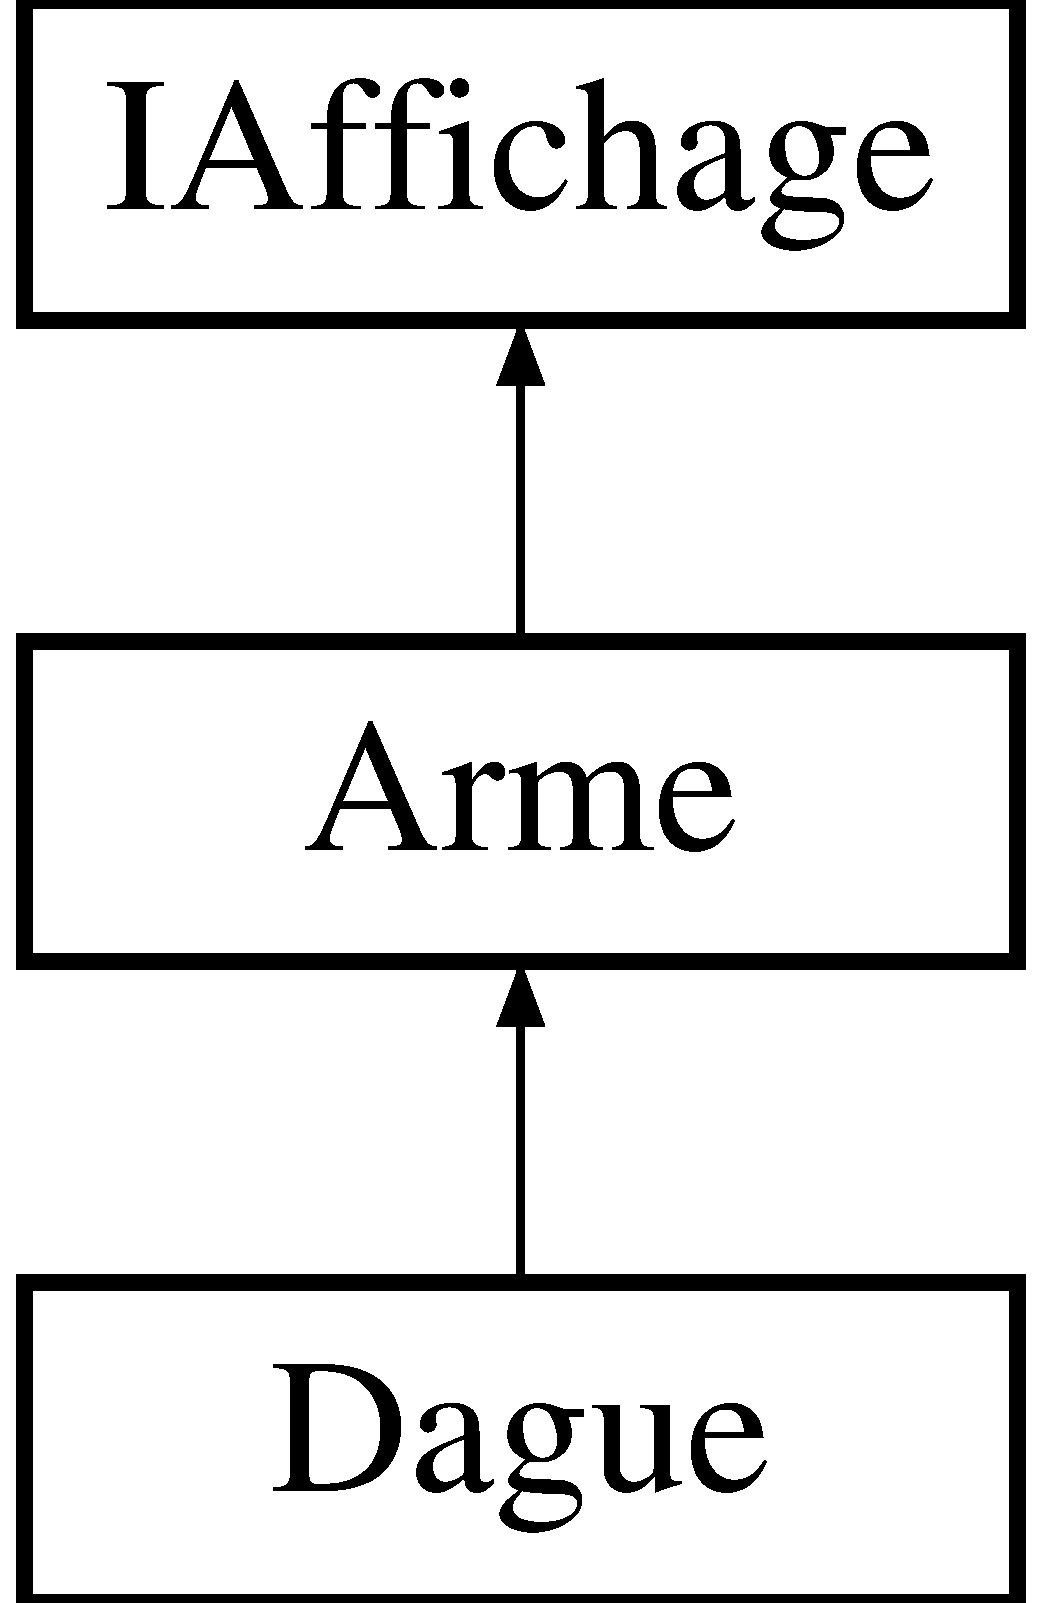
\includegraphics[height=3.000000cm]{class_dague}
\end{center}
\end{figure}
\subsection*{\-Public \-Member \-Functions}
\begin{DoxyCompactItemize}
\item 
\hyperlink{class_dague_a3568635e6ca934a13d86c6aa5bd3a28f}{\-Dague} ()
\item 
int \hyperlink{class_dague_afabd8cea0d60b3c8819c91005b395ca2}{get\-Id} ()
\item 
void \hyperlink{class_dague_a385f89995dd2e83f30891f2d356f8f48}{set\-Id} (int id)
\item 
string \hyperlink{class_dague_a96e7b1ec98a4c8995223f58cb7d151b7}{get\-Libelle} ()
\item 
void \hyperlink{class_dague_af23c946232782f7d1e305317c2ce0444}{set\-Libelle} (string l)
\item 
int \hyperlink{class_dague_a46d18edd393fa70d4724248c0f4dbe4a}{get\-Val\-Deg} ()
\item 
void \hyperlink{class_dague_af41cf1b4f02a2296a04d0e8fa858b5ff}{set\-Val\-Deg} (int v)
\end{DoxyCompactItemize}


\subsection{\-Detailed \-Description}
\-Classe \hyperlink{class_dague}{\-Dague}, hérite d'\hyperlink{class_arme}{\-Arme} 

\subsection{\-Constructor \& \-Destructor \-Documentation}
\hypertarget{class_dague_a3568635e6ca934a13d86c6aa5bd3a28f}{\index{\-Dague@{\-Dague}!\-Dague@{\-Dague}}
\index{\-Dague@{\-Dague}!Dague@{\-Dague}}
\subsubsection[{\-Dague}]{\setlength{\rightskip}{0pt plus 5cm}{\bf \-Dague\-::\-Dague} (
\begin{DoxyParamCaption}
{}
\end{DoxyParamCaption}
)\hspace{0.3cm}{\ttfamily  \mbox{[}inline\mbox{]}}}}\label{class_dague_a3568635e6ca934a13d86c6aa5bd3a28f}
\-Constructeur explicite initialisant les variables de la dague 

\subsection{\-Member \-Function \-Documentation}
\hypertarget{class_dague_afabd8cea0d60b3c8819c91005b395ca2}{\index{\-Dague@{\-Dague}!get\-Id@{get\-Id}}
\index{get\-Id@{get\-Id}!Dague@{\-Dague}}
\subsubsection[{get\-Id}]{\setlength{\rightskip}{0pt plus 5cm}int {\bf \-Dague\-::get\-Id} (
\begin{DoxyParamCaption}
{}
\end{DoxyParamCaption}
)\hspace{0.3cm}{\ttfamily  \mbox{[}inline\mbox{]}}}}\label{class_dague_afabd8cea0d60b3c8819c91005b395ca2}
\-Accesseur à l'identifiant de la dague 

\-Reimplemented from \hyperlink{class_arme_a6c957484697d9ad38ab1ed4361f3b8f4}{\-Arme}.

\hypertarget{class_dague_a96e7b1ec98a4c8995223f58cb7d151b7}{\index{\-Dague@{\-Dague}!get\-Libelle@{get\-Libelle}}
\index{get\-Libelle@{get\-Libelle}!Dague@{\-Dague}}
\subsubsection[{get\-Libelle}]{\setlength{\rightskip}{0pt plus 5cm}string {\bf \-Dague\-::get\-Libelle} (
\begin{DoxyParamCaption}
{}
\end{DoxyParamCaption}
)\hspace{0.3cm}{\ttfamily  \mbox{[}inline\mbox{]}}}}\label{class_dague_a96e7b1ec98a4c8995223f58cb7d151b7}
\-Accesseur au libellé de l'arme 

\-Reimplemented from \hyperlink{class_arme_a5e43d33d0e14da19fb37dc497474135b}{\-Arme}.

\hypertarget{class_dague_a46d18edd393fa70d4724248c0f4dbe4a}{\index{\-Dague@{\-Dague}!get\-Val\-Deg@{get\-Val\-Deg}}
\index{get\-Val\-Deg@{get\-Val\-Deg}!Dague@{\-Dague}}
\subsubsection[{get\-Val\-Deg}]{\setlength{\rightskip}{0pt plus 5cm}int {\bf \-Dague\-::get\-Val\-Deg} (
\begin{DoxyParamCaption}
{}
\end{DoxyParamCaption}
)\hspace{0.3cm}{\ttfamily  \mbox{[}inline\mbox{]}}}}\label{class_dague_a46d18edd393fa70d4724248c0f4dbe4a}
\-Accesseur à la valeur de dégâts de la dague \hypertarget{class_dague_a385f89995dd2e83f30891f2d356f8f48}{\index{\-Dague@{\-Dague}!set\-Id@{set\-Id}}
\index{set\-Id@{set\-Id}!Dague@{\-Dague}}
\subsubsection[{set\-Id}]{\setlength{\rightskip}{0pt plus 5cm}void {\bf \-Dague\-::set\-Id} (
\begin{DoxyParamCaption}
\item[{int}]{id}
\end{DoxyParamCaption}
)\hspace{0.3cm}{\ttfamily  \mbox{[}inline\mbox{]}}}}\label{class_dague_a385f89995dd2e83f30891f2d356f8f48}
\-Mutateur de l'identifiant de la dague 

\-Reimplemented from \hyperlink{class_arme_a332699f4c7b2dab9e38fccfddba7275b}{\-Arme}.

\hypertarget{class_dague_af23c946232782f7d1e305317c2ce0444}{\index{\-Dague@{\-Dague}!set\-Libelle@{set\-Libelle}}
\index{set\-Libelle@{set\-Libelle}!Dague@{\-Dague}}
\subsubsection[{set\-Libelle}]{\setlength{\rightskip}{0pt plus 5cm}void {\bf \-Dague\-::set\-Libelle} (
\begin{DoxyParamCaption}
\item[{string}]{l}
\end{DoxyParamCaption}
)\hspace{0.3cm}{\ttfamily  \mbox{[}inline\mbox{]}}}}\label{class_dague_af23c946232782f7d1e305317c2ce0444}
\-Mutateur du libellé de l'arme 

\-Reimplemented from \hyperlink{class_arme_ab38eebb032ab6773678ee40f152df6dd}{\-Arme}.

\hypertarget{class_dague_af41cf1b4f02a2296a04d0e8fa858b5ff}{\index{\-Dague@{\-Dague}!set\-Val\-Deg@{set\-Val\-Deg}}
\index{set\-Val\-Deg@{set\-Val\-Deg}!Dague@{\-Dague}}
\subsubsection[{set\-Val\-Deg}]{\setlength{\rightskip}{0pt plus 5cm}void {\bf \-Dague\-::set\-Val\-Deg} (
\begin{DoxyParamCaption}
\item[{int}]{v}
\end{DoxyParamCaption}
)\hspace{0.3cm}{\ttfamily  \mbox{[}inline\mbox{]}}}}\label{class_dague_af41cf1b4f02a2296a04d0e8fa858b5ff}
\-Mutateur de la valeur de dégâts de la dague 

\-The documentation for this class was generated from the following file\-:\begin{DoxyCompactItemize}
\item 
\-Projet\-P\-O\-O-\/master/\-Dague.\-cpp\end{DoxyCompactItemize}

\hypertarget{class_dimachaerus}{\section{\-Dimachaerus \-Class \-Reference}
\label{class_dimachaerus}\index{\-Dimachaerus@{\-Dimachaerus}}
}
\-Inheritance diagram for \-Dimachaerus\-:\begin{figure}[H]
\begin{center}
\leavevmode
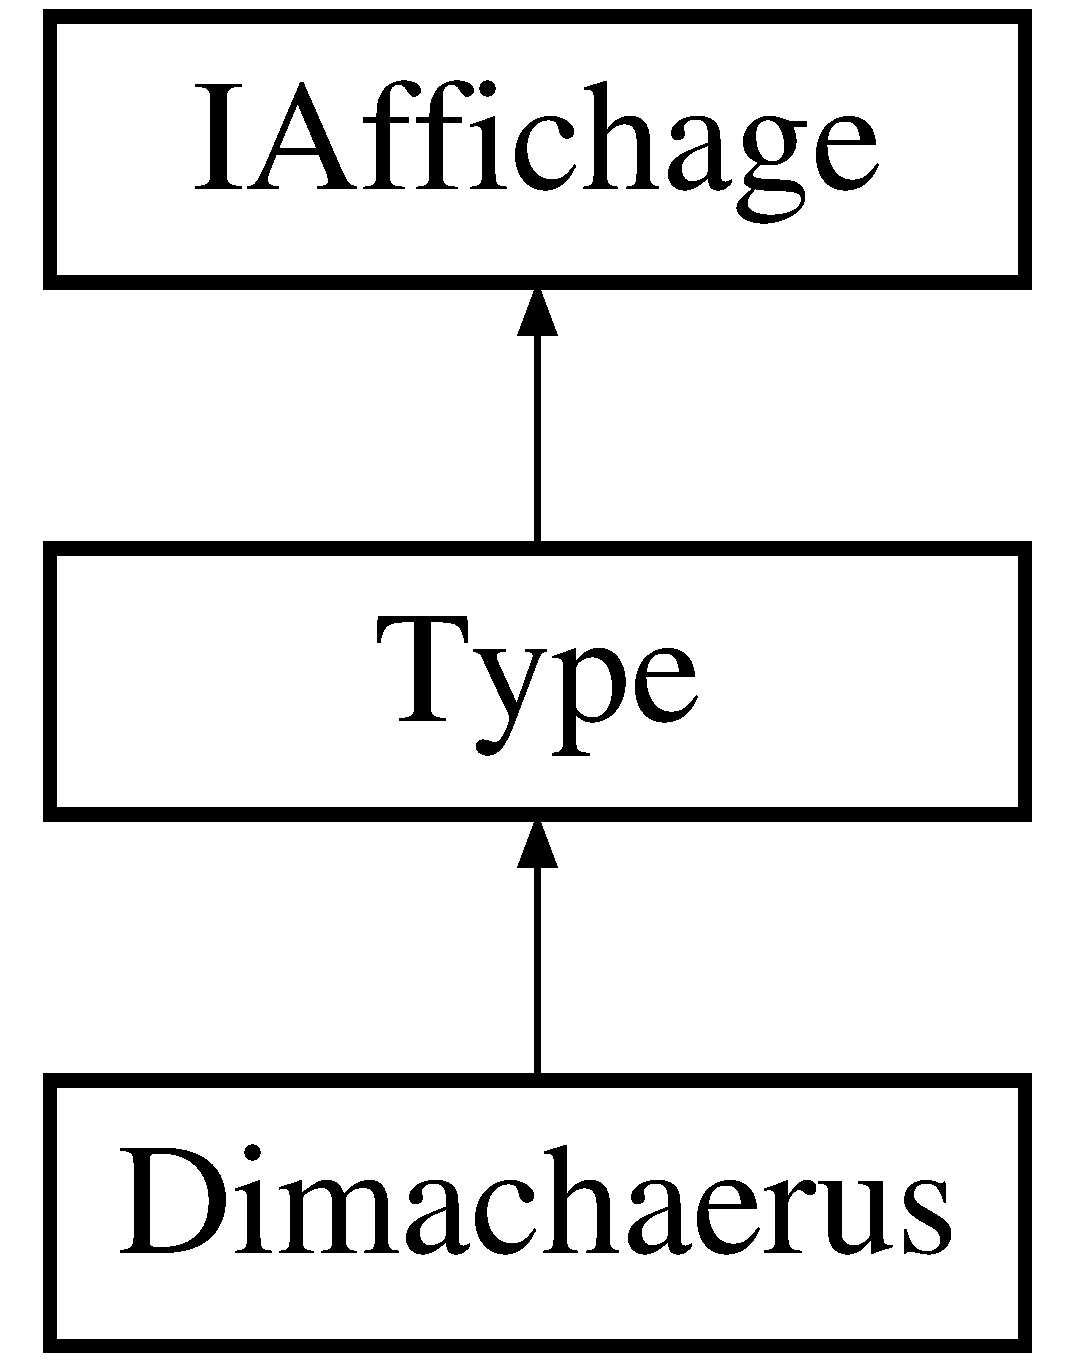
\includegraphics[height=3.000000cm]{class_dimachaerus}
\end{center}
\end{figure}
\subsection*{\-Public \-Member \-Functions}
\begin{DoxyCompactItemize}
\item 
\hyperlink{class_dimachaerus_a76b03d96de9077821ebc3b7ac043484d}{\-Dimachaerus} ()
\item 
int \hyperlink{class_dimachaerus_a134c3824829dbe4346fcfe149ca8b0bd}{get\-Id} ()
\item 
void \hyperlink{class_dimachaerus_a8977bd63eb521d2ee6c28e93807fafa6}{set\-Id} (int id)
\item 
string \hyperlink{class_dimachaerus_a66f91052ace7785e91077f28b12e0b51}{get\-Libelle} ()
\item 
void \hyperlink{class_dimachaerus_a77d28dc13bb678a8eb47f1b2f9cc8210}{set\-Libelle} (string l)
\end{DoxyCompactItemize}


\subsection{\-Detailed \-Description}
\-Classe \hyperlink{class_dimachaerus}{\-Dimachaerus}, hérite de \hyperlink{class_type}{\-Type} 

\subsection{\-Constructor \& \-Destructor \-Documentation}
\hypertarget{class_dimachaerus_a76b03d96de9077821ebc3b7ac043484d}{\index{\-Dimachaerus@{\-Dimachaerus}!\-Dimachaerus@{\-Dimachaerus}}
\index{\-Dimachaerus@{\-Dimachaerus}!Dimachaerus@{\-Dimachaerus}}
\subsubsection[{\-Dimachaerus}]{\setlength{\rightskip}{0pt plus 5cm}{\bf \-Dimachaerus\-::\-Dimachaerus} (
\begin{DoxyParamCaption}
{}
\end{DoxyParamCaption}
)\hspace{0.3cm}{\ttfamily  \mbox{[}inline\mbox{]}}}}\label{class_dimachaerus_a76b03d96de9077821ebc3b7ac043484d}
\-Constructeur explicite initialisant les variables du type 

\subsection{\-Member \-Function \-Documentation}
\hypertarget{class_dimachaerus_a134c3824829dbe4346fcfe149ca8b0bd}{\index{\-Dimachaerus@{\-Dimachaerus}!get\-Id@{get\-Id}}
\index{get\-Id@{get\-Id}!Dimachaerus@{\-Dimachaerus}}
\subsubsection[{get\-Id}]{\setlength{\rightskip}{0pt plus 5cm}int {\bf \-Dimachaerus\-::get\-Id} (
\begin{DoxyParamCaption}
{}
\end{DoxyParamCaption}
)\hspace{0.3cm}{\ttfamily  \mbox{[}inline\mbox{]}}}}\label{class_dimachaerus_a134c3824829dbe4346fcfe149ca8b0bd}
\-Accesseur à l'identifiant du type 

\-Reimplemented from \hyperlink{class_type_aba890fe7677f58f7135ec0cfe1b7c926}{\-Type}.

\hypertarget{class_dimachaerus_a66f91052ace7785e91077f28b12e0b51}{\index{\-Dimachaerus@{\-Dimachaerus}!get\-Libelle@{get\-Libelle}}
\index{get\-Libelle@{get\-Libelle}!Dimachaerus@{\-Dimachaerus}}
\subsubsection[{get\-Libelle}]{\setlength{\rightskip}{0pt plus 5cm}string {\bf \-Dimachaerus\-::get\-Libelle} (
\begin{DoxyParamCaption}
{}
\end{DoxyParamCaption}
)\hspace{0.3cm}{\ttfamily  \mbox{[}inline\mbox{]}}}}\label{class_dimachaerus_a66f91052ace7785e91077f28b12e0b51}
\-Accesseur au libellé du type 

\-Reimplemented from \hyperlink{class_type_a38a529eb6a80a3d3cb801996cc9f41f0}{\-Type}.

\hypertarget{class_dimachaerus_a8977bd63eb521d2ee6c28e93807fafa6}{\index{\-Dimachaerus@{\-Dimachaerus}!set\-Id@{set\-Id}}
\index{set\-Id@{set\-Id}!Dimachaerus@{\-Dimachaerus}}
\subsubsection[{set\-Id}]{\setlength{\rightskip}{0pt plus 5cm}void {\bf \-Dimachaerus\-::set\-Id} (
\begin{DoxyParamCaption}
\item[{int}]{id}
\end{DoxyParamCaption}
)\hspace{0.3cm}{\ttfamily  \mbox{[}inline\mbox{]}}}}\label{class_dimachaerus_a8977bd63eb521d2ee6c28e93807fafa6}
\-Mutateur de l'identifiant du type 

\-Reimplemented from \hyperlink{class_type_ab9b8158dca9be6184557382ec98ec4f7}{\-Type}.

\hypertarget{class_dimachaerus_a77d28dc13bb678a8eb47f1b2f9cc8210}{\index{\-Dimachaerus@{\-Dimachaerus}!set\-Libelle@{set\-Libelle}}
\index{set\-Libelle@{set\-Libelle}!Dimachaerus@{\-Dimachaerus}}
\subsubsection[{set\-Libelle}]{\setlength{\rightskip}{0pt plus 5cm}void {\bf \-Dimachaerus\-::set\-Libelle} (
\begin{DoxyParamCaption}
\item[{string}]{l}
\end{DoxyParamCaption}
)\hspace{0.3cm}{\ttfamily  \mbox{[}inline\mbox{]}}}}\label{class_dimachaerus_a77d28dc13bb678a8eb47f1b2f9cc8210}
\-Mutateur du libellé du type 

\-Reimplemented from \hyperlink{class_type_af475df921624fe329aaa6b19bd1ed2e1}{\-Type}.



\-The documentation for this class was generated from the following file\-:\begin{DoxyCompactItemize}
\item 
\-Projet\-P\-O\-O-\/master/\-Dimachaerus.\-cpp\end{DoxyCompactItemize}

\hypertarget{class_effet}{\section{\-Effet \-Class \-Reference}
\label{class_effet}\index{\-Effet@{\-Effet}}
}
\-Inheritance diagram for \-Effet\-:\begin{figure}[H]
\begin{center}
\leavevmode
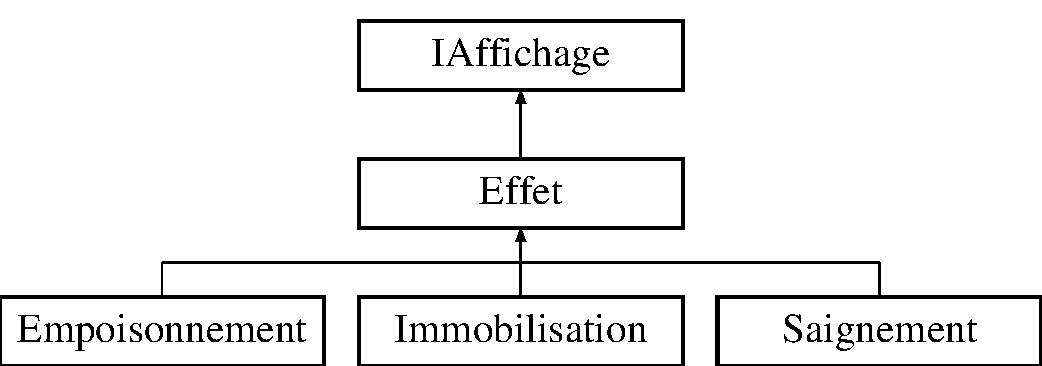
\includegraphics[height=3.000000cm]{class_effet}
\end{center}
\end{figure}
\subsection*{\-Public \-Member \-Functions}
\begin{DoxyCompactItemize}
\item 
int \hyperlink{class_effet_a509c2d845776b583280b4418585d9ec2}{get\-Id} ()
\item 
void \hyperlink{class_effet_a1e880a5364a175e90dae7cbfdc103e02}{set\-Id} (int id)
\item 
string \hyperlink{class_effet_a1817f59e4c17c91103ae4031868dfd97}{get\-Libelle} ()
\item 
void \hyperlink{class_effet_a8470c57c7d69b4023c5230cdca79631d}{set\-Libelle} (string l)
\item 
int \hyperlink{class_effet_ae98c2a33fcd29629e3c7cd6e8ab8fcd8}{get\-Nb\-Tours\-Max} ()
\item 
void \hyperlink{class_effet_a12959d98a93ca835aedd8b7ed84e5a61}{set\-Nb\-Tours\-Max} (int n)
\item 
virtual void \hyperlink{class_effet_afa8ada372b122c1447ee6ac51b551f6a}{afficher\-Info} ()
\end{DoxyCompactItemize}


\subsection{\-Detailed \-Description}
\-Classe mère \hyperlink{class_effet}{\-Effet}, tous les effets héritent de celle-\/ci \-Implémente l'interface \hyperlink{class_i_affichage}{\-I\-Affichage} 

\subsection{\-Member \-Function \-Documentation}
\hypertarget{class_effet_afa8ada372b122c1447ee6ac51b551f6a}{\index{\-Effet@{\-Effet}!afficher\-Info@{afficher\-Info}}
\index{afficher\-Info@{afficher\-Info}!Effet@{\-Effet}}
\subsubsection[{afficher\-Info}]{\setlength{\rightskip}{0pt plus 5cm}virtual void {\bf \-Effet\-::afficher\-Info} (
\begin{DoxyParamCaption}
{}
\end{DoxyParamCaption}
)\hspace{0.3cm}{\ttfamily  \mbox{[}inline, virtual\mbox{]}}}}\label{class_effet_afa8ada372b122c1447ee6ac51b551f6a}
\-Procédure d'affichage d'informations, redéfinit celle de l'interface \hyperlink{class_i_affichage}{\-I\-Affichage} 

\-Implements \hyperlink{class_i_affichage_a6123c1cb9079f712b48c0b8bf62e14ef}{\-I\-Affichage}.

\hypertarget{class_effet_a509c2d845776b583280b4418585d9ec2}{\index{\-Effet@{\-Effet}!get\-Id@{get\-Id}}
\index{get\-Id@{get\-Id}!Effet@{\-Effet}}
\subsubsection[{get\-Id}]{\setlength{\rightskip}{0pt plus 5cm}int {\bf \-Effet\-::get\-Id} (
\begin{DoxyParamCaption}
{}
\end{DoxyParamCaption}
)\hspace{0.3cm}{\ttfamily  \mbox{[}inline\mbox{]}}}}\label{class_effet_a509c2d845776b583280b4418585d9ec2}
\-Accesseur à l'identifiant de l'effet 

\-Reimplemented in \hyperlink{class_empoisonnement_aca251add204972489663e8a6a56525ac}{\-Empoisonnement}, \hyperlink{class_saignement_a57ccf17cade8c253a7ee99e7f816eb10}{\-Saignement}, and \hyperlink{class_immobilisation_a4ffaa8356838b9bc202e16136bed7c93}{\-Immobilisation}.

\hypertarget{class_effet_a1817f59e4c17c91103ae4031868dfd97}{\index{\-Effet@{\-Effet}!get\-Libelle@{get\-Libelle}}
\index{get\-Libelle@{get\-Libelle}!Effet@{\-Effet}}
\subsubsection[{get\-Libelle}]{\setlength{\rightskip}{0pt plus 5cm}string {\bf \-Effet\-::get\-Libelle} (
\begin{DoxyParamCaption}
{}
\end{DoxyParamCaption}
)\hspace{0.3cm}{\ttfamily  \mbox{[}inline\mbox{]}}}}\label{class_effet_a1817f59e4c17c91103ae4031868dfd97}
\-Accesseur au libellé l'effet 

\-Reimplemented in \hyperlink{class_empoisonnement_a787da32b563d6f18bb8307d59bbfb9ec}{\-Empoisonnement}, \hyperlink{class_saignement_aca2c045c2faa9384b6cf25ec3c11af28}{\-Saignement}, and \hyperlink{class_immobilisation_a77ed10535746670f2e0cdfcf385884a2}{\-Immobilisation}.

\hypertarget{class_effet_ae98c2a33fcd29629e3c7cd6e8ab8fcd8}{\index{\-Effet@{\-Effet}!get\-Nb\-Tours\-Max@{get\-Nb\-Tours\-Max}}
\index{get\-Nb\-Tours\-Max@{get\-Nb\-Tours\-Max}!Effet@{\-Effet}}
\subsubsection[{get\-Nb\-Tours\-Max}]{\setlength{\rightskip}{0pt plus 5cm}int {\bf \-Effet\-::get\-Nb\-Tours\-Max} (
\begin{DoxyParamCaption}
{}
\end{DoxyParamCaption}
)\hspace{0.3cm}{\ttfamily  \mbox{[}inline\mbox{]}}}}\label{class_effet_ae98c2a33fcd29629e3c7cd6e8ab8fcd8}
\-Accesseur à la durée maximale, en tours, de l'effet 

\-Reimplemented in \hyperlink{class_empoisonnement_a10bcef58e5f423cf1b957591787fb157}{\-Empoisonnement}, \hyperlink{class_saignement_a498bf00562314e4094be4004e5bc653a}{\-Saignement}, and \hyperlink{class_immobilisation_ae0baa3a4c8e7e39ba0646c5afda69ce8}{\-Immobilisation}.

\hypertarget{class_effet_a1e880a5364a175e90dae7cbfdc103e02}{\index{\-Effet@{\-Effet}!set\-Id@{set\-Id}}
\index{set\-Id@{set\-Id}!Effet@{\-Effet}}
\subsubsection[{set\-Id}]{\setlength{\rightskip}{0pt plus 5cm}void {\bf \-Effet\-::set\-Id} (
\begin{DoxyParamCaption}
\item[{int}]{id}
\end{DoxyParamCaption}
)\hspace{0.3cm}{\ttfamily  \mbox{[}inline\mbox{]}}}}\label{class_effet_a1e880a5364a175e90dae7cbfdc103e02}
\-Mutateur de l'identifiant de l'effet 

\-Reimplemented in \hyperlink{class_empoisonnement_a0bd14f04931bcd9f926036ab2ece8ce6}{\-Empoisonnement}, \hyperlink{class_saignement_af9d66877c7e2aff769b4bc48f4bb82e4}{\-Saignement}, and \hyperlink{class_immobilisation_a1b0d3098ec798b0c8d46ff51aa0c0db2}{\-Immobilisation}.

\hypertarget{class_effet_a8470c57c7d69b4023c5230cdca79631d}{\index{\-Effet@{\-Effet}!set\-Libelle@{set\-Libelle}}
\index{set\-Libelle@{set\-Libelle}!Effet@{\-Effet}}
\subsubsection[{set\-Libelle}]{\setlength{\rightskip}{0pt plus 5cm}void {\bf \-Effet\-::set\-Libelle} (
\begin{DoxyParamCaption}
\item[{string}]{l}
\end{DoxyParamCaption}
)\hspace{0.3cm}{\ttfamily  \mbox{[}inline\mbox{]}}}}\label{class_effet_a8470c57c7d69b4023c5230cdca79631d}
\-Mutateur du libellé de l'effet 

\-Reimplemented in \hyperlink{class_empoisonnement_a0ab7a1e8a917a0f050832819b3804a96}{\-Empoisonnement}, \hyperlink{class_saignement_a2c9f7ffb81aa8848564389580c4f7112}{\-Saignement}, and \hyperlink{class_immobilisation_a32e8e9379388f0a492fe0fd97ec9c304}{\-Immobilisation}.

\hypertarget{class_effet_a12959d98a93ca835aedd8b7ed84e5a61}{\index{\-Effet@{\-Effet}!set\-Nb\-Tours\-Max@{set\-Nb\-Tours\-Max}}
\index{set\-Nb\-Tours\-Max@{set\-Nb\-Tours\-Max}!Effet@{\-Effet}}
\subsubsection[{set\-Nb\-Tours\-Max}]{\setlength{\rightskip}{0pt plus 5cm}void {\bf \-Effet\-::set\-Nb\-Tours\-Max} (
\begin{DoxyParamCaption}
\item[{int}]{n}
\end{DoxyParamCaption}
)\hspace{0.3cm}{\ttfamily  \mbox{[}inline\mbox{]}}}}\label{class_effet_a12959d98a93ca835aedd8b7ed84e5a61}
\-Mutateur de la durée maximale, en tours, de l'effet 

\-Reimplemented in \hyperlink{class_empoisonnement_a52a3cc1746ccacb1c29e6bd8a2aecf94}{\-Empoisonnement}, \hyperlink{class_saignement_ae31708c65c109f4169d1e79fca31eade}{\-Saignement}, and \hyperlink{class_immobilisation_a2b4a2b1ee2ef7b0e11ca3cf92ec4caad}{\-Immobilisation}.



\-The documentation for this class was generated from the following file\-:\begin{DoxyCompactItemize}
\item 
\-Projet\-P\-O\-O-\/master/\-Effet.\-cpp\end{DoxyCompactItemize}

\hypertarget{class_empoisonnement}{\section{\-Empoisonnement \-Class \-Reference}
\label{class_empoisonnement}\index{\-Empoisonnement@{\-Empoisonnement}}
}
\-Inheritance diagram for \-Empoisonnement\-:\begin{figure}[H]
\begin{center}
\leavevmode
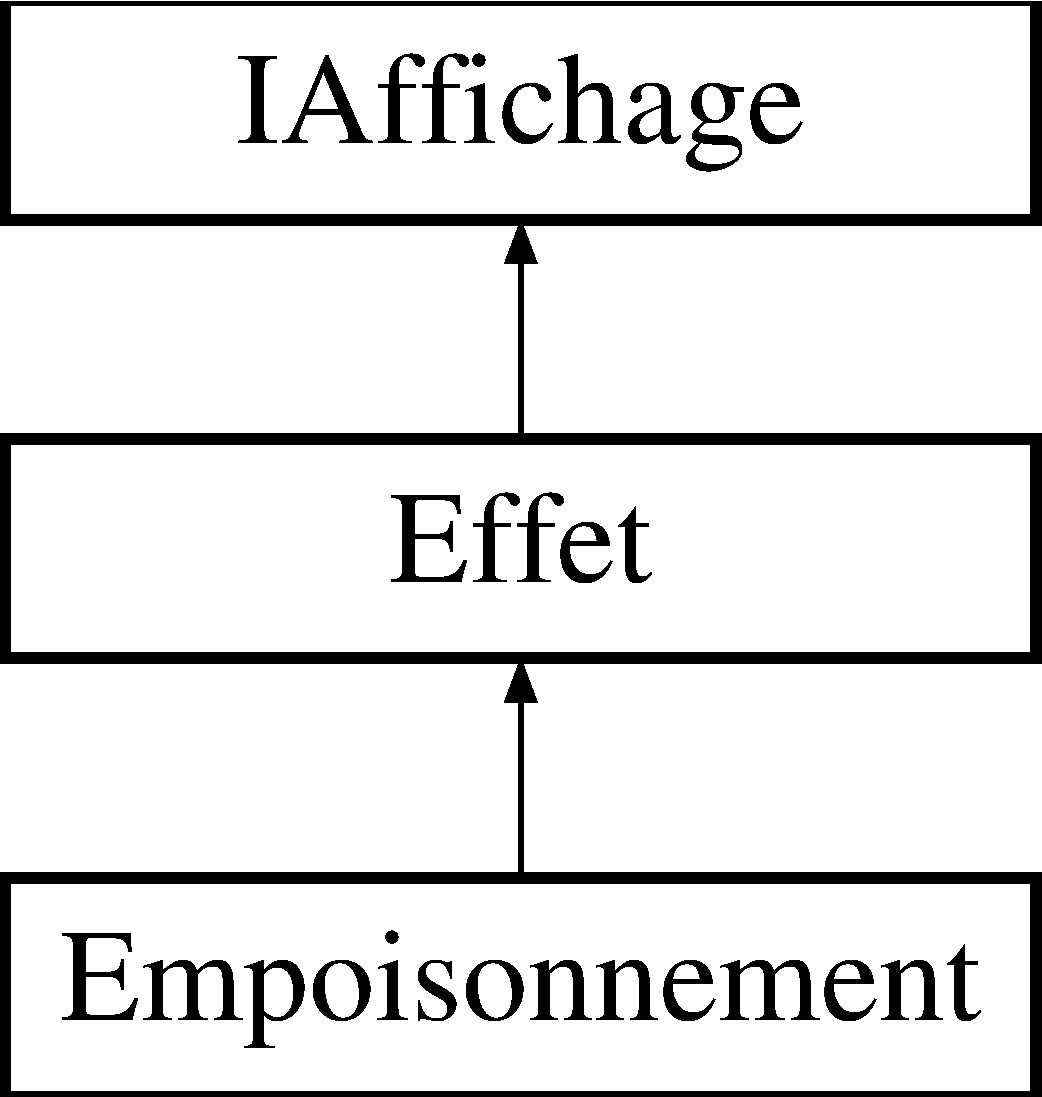
\includegraphics[height=3.000000cm]{class_empoisonnement}
\end{center}
\end{figure}
\subsection*{\-Public \-Member \-Functions}
\begin{DoxyCompactItemize}
\item 
\hyperlink{class_empoisonnement_a10f418f15faeaf3f5940234b282f0638}{\-Empoisonnement} ()
\item 
int \hyperlink{class_empoisonnement_aca251add204972489663e8a6a56525ac}{get\-Id} ()
\item 
void \hyperlink{class_empoisonnement_a0bd14f04931bcd9f926036ab2ece8ce6}{set\-Id} (int id)
\item 
string \hyperlink{class_empoisonnement_a787da32b563d6f18bb8307d59bbfb9ec}{get\-Libelle} ()
\item 
void \hyperlink{class_empoisonnement_a0ab7a1e8a917a0f050832819b3804a96}{set\-Libelle} (string l)
\item 
int \hyperlink{class_empoisonnement_a10bcef58e5f423cf1b957591787fb157}{get\-Nb\-Tours\-Max} ()
\item 
void \hyperlink{class_empoisonnement_a52a3cc1746ccacb1c29e6bd8a2aecf94}{set\-Nb\-Tours\-Max} (int n)
\item 
int \hyperlink{class_empoisonnement_a4ba692ca3d6fd64653471c6a757c1701}{get\-Val\-Deg} ()
\item 
void \hyperlink{class_empoisonnement_a15b5148b3e38af152c74f4fe5bf85c6c}{set\-Val\-Deg} (int v)
\end{DoxyCompactItemize}


\subsection{\-Detailed \-Description}
\-Classe \hyperlink{class_empoisonnement}{\-Empoisonnement}, hérite d'\hyperlink{class_effet}{\-Effet} 

\subsection{\-Constructor \& \-Destructor \-Documentation}
\hypertarget{class_empoisonnement_a10f418f15faeaf3f5940234b282f0638}{\index{\-Empoisonnement@{\-Empoisonnement}!\-Empoisonnement@{\-Empoisonnement}}
\index{\-Empoisonnement@{\-Empoisonnement}!Empoisonnement@{\-Empoisonnement}}
\subsubsection[{\-Empoisonnement}]{\setlength{\rightskip}{0pt plus 5cm}{\bf \-Empoisonnement\-::\-Empoisonnement} (
\begin{DoxyParamCaption}
{}
\end{DoxyParamCaption}
)\hspace{0.3cm}{\ttfamily  \mbox{[}inline\mbox{]}}}}\label{class_empoisonnement_a10f418f15faeaf3f5940234b282f0638}
\-Constructeur explicite initialisant les variables de l'effet 

\subsection{\-Member \-Function \-Documentation}
\hypertarget{class_empoisonnement_aca251add204972489663e8a6a56525ac}{\index{\-Empoisonnement@{\-Empoisonnement}!get\-Id@{get\-Id}}
\index{get\-Id@{get\-Id}!Empoisonnement@{\-Empoisonnement}}
\subsubsection[{get\-Id}]{\setlength{\rightskip}{0pt plus 5cm}int {\bf \-Empoisonnement\-::get\-Id} (
\begin{DoxyParamCaption}
{}
\end{DoxyParamCaption}
)\hspace{0.3cm}{\ttfamily  \mbox{[}inline\mbox{]}}}}\label{class_empoisonnement_aca251add204972489663e8a6a56525ac}
\-Accesseur à l'identifiant de l'effet 

\-Reimplemented from \hyperlink{class_effet_a509c2d845776b583280b4418585d9ec2}{\-Effet}.

\hypertarget{class_empoisonnement_a787da32b563d6f18bb8307d59bbfb9ec}{\index{\-Empoisonnement@{\-Empoisonnement}!get\-Libelle@{get\-Libelle}}
\index{get\-Libelle@{get\-Libelle}!Empoisonnement@{\-Empoisonnement}}
\subsubsection[{get\-Libelle}]{\setlength{\rightskip}{0pt plus 5cm}string {\bf \-Empoisonnement\-::get\-Libelle} (
\begin{DoxyParamCaption}
{}
\end{DoxyParamCaption}
)\hspace{0.3cm}{\ttfamily  \mbox{[}inline\mbox{]}}}}\label{class_empoisonnement_a787da32b563d6f18bb8307d59bbfb9ec}
\-Accesseur au libellé de l'effet 

\-Reimplemented from \hyperlink{class_effet_a1817f59e4c17c91103ae4031868dfd97}{\-Effet}.

\hypertarget{class_empoisonnement_a10bcef58e5f423cf1b957591787fb157}{\index{\-Empoisonnement@{\-Empoisonnement}!get\-Nb\-Tours\-Max@{get\-Nb\-Tours\-Max}}
\index{get\-Nb\-Tours\-Max@{get\-Nb\-Tours\-Max}!Empoisonnement@{\-Empoisonnement}}
\subsubsection[{get\-Nb\-Tours\-Max}]{\setlength{\rightskip}{0pt plus 5cm}int {\bf \-Empoisonnement\-::get\-Nb\-Tours\-Max} (
\begin{DoxyParamCaption}
{}
\end{DoxyParamCaption}
)\hspace{0.3cm}{\ttfamily  \mbox{[}inline\mbox{]}}}}\label{class_empoisonnement_a10bcef58e5f423cf1b957591787fb157}
\-Accesseur à la durée maximale, en tours, de l'effet 

\-Reimplemented from \hyperlink{class_effet_ae98c2a33fcd29629e3c7cd6e8ab8fcd8}{\-Effet}.

\hypertarget{class_empoisonnement_a4ba692ca3d6fd64653471c6a757c1701}{\index{\-Empoisonnement@{\-Empoisonnement}!get\-Val\-Deg@{get\-Val\-Deg}}
\index{get\-Val\-Deg@{get\-Val\-Deg}!Empoisonnement@{\-Empoisonnement}}
\subsubsection[{get\-Val\-Deg}]{\setlength{\rightskip}{0pt plus 5cm}int {\bf \-Empoisonnement\-::get\-Val\-Deg} (
\begin{DoxyParamCaption}
{}
\end{DoxyParamCaption}
)\hspace{0.3cm}{\ttfamily  \mbox{[}inline\mbox{]}}}}\label{class_empoisonnement_a4ba692ca3d6fd64653471c6a757c1701}
\-Accesseur à la valeur de dégâts de l'effet \hypertarget{class_empoisonnement_a0bd14f04931bcd9f926036ab2ece8ce6}{\index{\-Empoisonnement@{\-Empoisonnement}!set\-Id@{set\-Id}}
\index{set\-Id@{set\-Id}!Empoisonnement@{\-Empoisonnement}}
\subsubsection[{set\-Id}]{\setlength{\rightskip}{0pt plus 5cm}void {\bf \-Empoisonnement\-::set\-Id} (
\begin{DoxyParamCaption}
\item[{int}]{id}
\end{DoxyParamCaption}
)\hspace{0.3cm}{\ttfamily  \mbox{[}inline\mbox{]}}}}\label{class_empoisonnement_a0bd14f04931bcd9f926036ab2ece8ce6}
\-Mutateur de l'identifiant de l'effet 

\-Reimplemented from \hyperlink{class_effet_a1e880a5364a175e90dae7cbfdc103e02}{\-Effet}.

\hypertarget{class_empoisonnement_a0ab7a1e8a917a0f050832819b3804a96}{\index{\-Empoisonnement@{\-Empoisonnement}!set\-Libelle@{set\-Libelle}}
\index{set\-Libelle@{set\-Libelle}!Empoisonnement@{\-Empoisonnement}}
\subsubsection[{set\-Libelle}]{\setlength{\rightskip}{0pt plus 5cm}void {\bf \-Empoisonnement\-::set\-Libelle} (
\begin{DoxyParamCaption}
\item[{string}]{l}
\end{DoxyParamCaption}
)\hspace{0.3cm}{\ttfamily  \mbox{[}inline\mbox{]}}}}\label{class_empoisonnement_a0ab7a1e8a917a0f050832819b3804a96}
\-Mutateur du libellé de l'effet 

\-Reimplemented from \hyperlink{class_effet_a8470c57c7d69b4023c5230cdca79631d}{\-Effet}.

\hypertarget{class_empoisonnement_a52a3cc1746ccacb1c29e6bd8a2aecf94}{\index{\-Empoisonnement@{\-Empoisonnement}!set\-Nb\-Tours\-Max@{set\-Nb\-Tours\-Max}}
\index{set\-Nb\-Tours\-Max@{set\-Nb\-Tours\-Max}!Empoisonnement@{\-Empoisonnement}}
\subsubsection[{set\-Nb\-Tours\-Max}]{\setlength{\rightskip}{0pt plus 5cm}void {\bf \-Empoisonnement\-::set\-Nb\-Tours\-Max} (
\begin{DoxyParamCaption}
\item[{int}]{n}
\end{DoxyParamCaption}
)\hspace{0.3cm}{\ttfamily  \mbox{[}inline\mbox{]}}}}\label{class_empoisonnement_a52a3cc1746ccacb1c29e6bd8a2aecf94}
\-Mutateur de la durée maximale, en tours, de l'effet 

\-Reimplemented from \hyperlink{class_effet_a12959d98a93ca835aedd8b7ed84e5a61}{\-Effet}.

\hypertarget{class_empoisonnement_a15b5148b3e38af152c74f4fe5bf85c6c}{\index{\-Empoisonnement@{\-Empoisonnement}!set\-Val\-Deg@{set\-Val\-Deg}}
\index{set\-Val\-Deg@{set\-Val\-Deg}!Empoisonnement@{\-Empoisonnement}}
\subsubsection[{set\-Val\-Deg}]{\setlength{\rightskip}{0pt plus 5cm}void {\bf \-Empoisonnement\-::set\-Val\-Deg} (
\begin{DoxyParamCaption}
\item[{int}]{v}
\end{DoxyParamCaption}
)\hspace{0.3cm}{\ttfamily  \mbox{[}inline\mbox{]}}}}\label{class_empoisonnement_a15b5148b3e38af152c74f4fe5bf85c6c}
\-Mutateur de la valeur de dégâts de l'effet 

\-The documentation for this class was generated from the following file\-:\begin{DoxyCompactItemize}
\item 
\-Projet\-P\-O\-O-\/master/\-Empoisonnement.\-cpp\end{DoxyCompactItemize}

\hypertarget{class_equipement}{\section{\-Equipement \-Class \-Reference}
\label{class_equipement}\index{\-Equipement@{\-Equipement}}
}
\-Inheritance diagram for \-Equipement\-:\begin{figure}[H]
\begin{center}
\leavevmode
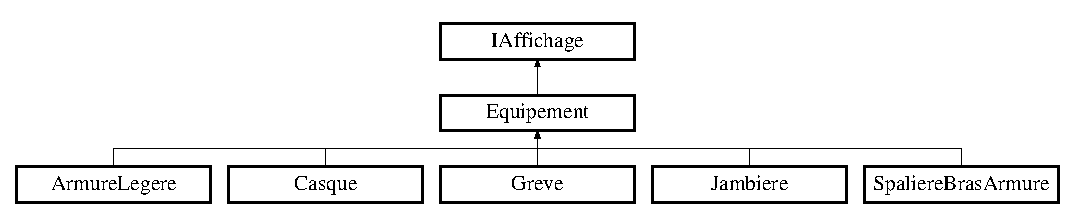
\includegraphics[height=2.488889cm]{class_equipement}
\end{center}
\end{figure}
\subsection*{\-Public \-Member \-Functions}
\begin{DoxyCompactItemize}
\item 
int \hyperlink{class_equipement_abc38941f5a9deed943b7a83ce69539c3}{get\-Id} ()
\item 
void \hyperlink{class_equipement_a98208826ad05cbc38211e9f70bd908c5}{set\-Id} (int id)
\item 
string \hyperlink{class_equipement_ab00ec565966647bf6edeb1a9df430aa6}{get\-Libelle} ()
\item 
void \hyperlink{class_equipement_aea246b68c747bd5ec84ca8ce4c4c7b40}{set\-Libelle} (string l)
\item 
int \hyperlink{class_equipement_a7b3003f4da24a94bfec94555e35e772c}{get\-Val\-Def} ()
\item 
void \hyperlink{class_equipement_ad9940c901b3a96b91c5c3f24713face5}{set\-Val\-Def} (int v)
\item 
virtual void \hyperlink{class_equipement_a8db0d237091051e004df0e2274e9e015}{afficher\-Info} ()
\end{DoxyCompactItemize}


\subsection{\-Detailed \-Description}
\-Classe mère \hyperlink{class_equipement}{\-Equipement}, tous les équipements héritent de celle-\/ci \-Implémente l'interface \hyperlink{class_i_affichage}{\-I\-Affichage} 

\subsection{\-Member \-Function \-Documentation}
\hypertarget{class_equipement_a8db0d237091051e004df0e2274e9e015}{\index{\-Equipement@{\-Equipement}!afficher\-Info@{afficher\-Info}}
\index{afficher\-Info@{afficher\-Info}!Equipement@{\-Equipement}}
\subsubsection[{afficher\-Info}]{\setlength{\rightskip}{0pt plus 5cm}virtual void {\bf \-Equipement\-::afficher\-Info} (
\begin{DoxyParamCaption}
{}
\end{DoxyParamCaption}
)\hspace{0.3cm}{\ttfamily  \mbox{[}inline, virtual\mbox{]}}}}\label{class_equipement_a8db0d237091051e004df0e2274e9e015}
\-Procédure d'affichage d'informations, redéfinit celle de l'interface \hyperlink{class_i_affichage}{\-I\-Affichage} 

\-Implements \hyperlink{class_i_affichage_a6123c1cb9079f712b48c0b8bf62e14ef}{\-I\-Affichage}.

\hypertarget{class_equipement_abc38941f5a9deed943b7a83ce69539c3}{\index{\-Equipement@{\-Equipement}!get\-Id@{get\-Id}}
\index{get\-Id@{get\-Id}!Equipement@{\-Equipement}}
\subsubsection[{get\-Id}]{\setlength{\rightskip}{0pt plus 5cm}int {\bf \-Equipement\-::get\-Id} (
\begin{DoxyParamCaption}
{}
\end{DoxyParamCaption}
)\hspace{0.3cm}{\ttfamily  \mbox{[}inline\mbox{]}}}}\label{class_equipement_abc38941f5a9deed943b7a83ce69539c3}
\-Accesseur à l'identifiant de l'équipement 

\-Reimplemented in \hyperlink{class_armure_legere_a605de63de0fbb64f4170865ca8e7e851}{\-Armure\-Legere}, \hyperlink{class_casque_a274f8d36daf144145d716bb4f09d92ae}{\-Casque}, \hyperlink{class_greve_a9d1f9157ba388f329a51ba447950c257}{\-Greve}, \hyperlink{class_jambiere_af22ba3e8b9617ff4e5930509b9adb9f4}{\-Jambiere}, and \hyperlink{class_spaliere_bras_armure_aced30cd7ce6d4b4cf0276ebd174164b5}{\-Spaliere\-Bras\-Armure}.

\hypertarget{class_equipement_ab00ec565966647bf6edeb1a9df430aa6}{\index{\-Equipement@{\-Equipement}!get\-Libelle@{get\-Libelle}}
\index{get\-Libelle@{get\-Libelle}!Equipement@{\-Equipement}}
\subsubsection[{get\-Libelle}]{\setlength{\rightskip}{0pt plus 5cm}string {\bf \-Equipement\-::get\-Libelle} (
\begin{DoxyParamCaption}
{}
\end{DoxyParamCaption}
)\hspace{0.3cm}{\ttfamily  \mbox{[}inline\mbox{]}}}}\label{class_equipement_ab00ec565966647bf6edeb1a9df430aa6}
\-Accesseur au libellé de l'équipement 

\-Reimplemented in \hyperlink{class_armure_legere_a6201feeb0e1c65d756a2dc064a72b1c4}{\-Armure\-Legere}, \hyperlink{class_casque_a408f8a20ef9a6513e3798975926c329b}{\-Casque}, \hyperlink{class_greve_a11a9352790169fab9893ce8ef96f657c}{\-Greve}, \hyperlink{class_jambiere_ad798b9a2d5e43a09aedc606eec7df9a2}{\-Jambiere}, and \hyperlink{class_spaliere_bras_armure_a5cccfb1ec9c35ce6ff193b956922ac0b}{\-Spaliere\-Bras\-Armure}.

\hypertarget{class_equipement_a7b3003f4da24a94bfec94555e35e772c}{\index{\-Equipement@{\-Equipement}!get\-Val\-Def@{get\-Val\-Def}}
\index{get\-Val\-Def@{get\-Val\-Def}!Equipement@{\-Equipement}}
\subsubsection[{get\-Val\-Def}]{\setlength{\rightskip}{0pt plus 5cm}int {\bf \-Equipement\-::get\-Val\-Def} (
\begin{DoxyParamCaption}
{}
\end{DoxyParamCaption}
)\hspace{0.3cm}{\ttfamily  \mbox{[}inline\mbox{]}}}}\label{class_equipement_a7b3003f4da24a94bfec94555e35e772c}
\-Accesseur à la valeur de défense de l'équipement 

\-Reimplemented in \hyperlink{class_armure_legere_aa455d08100ac7895b1d1d7b61c92da3f}{\-Armure\-Legere}, \hyperlink{class_casque_a899bc40890f9afaccc665bc816864084}{\-Casque}, \hyperlink{class_greve_ad03dddd443d2452134827983aa3541ec}{\-Greve}, \hyperlink{class_jambiere_a05c9fa271a51edccbd559a29ca45fe60}{\-Jambiere}, and \hyperlink{class_spaliere_bras_armure_af0f4b0c780083719852fcff96bc0083f}{\-Spaliere\-Bras\-Armure}.

\hypertarget{class_equipement_a98208826ad05cbc38211e9f70bd908c5}{\index{\-Equipement@{\-Equipement}!set\-Id@{set\-Id}}
\index{set\-Id@{set\-Id}!Equipement@{\-Equipement}}
\subsubsection[{set\-Id}]{\setlength{\rightskip}{0pt plus 5cm}void {\bf \-Equipement\-::set\-Id} (
\begin{DoxyParamCaption}
\item[{int}]{id}
\end{DoxyParamCaption}
)\hspace{0.3cm}{\ttfamily  \mbox{[}inline\mbox{]}}}}\label{class_equipement_a98208826ad05cbc38211e9f70bd908c5}
\-Mutateur de l'identifiant de l'équipement 

\-Reimplemented in \hyperlink{class_armure_legere_a407cda69c45c312f8fa8df854504f717}{\-Armure\-Legere}, \hyperlink{class_casque_aa6c352baa2c050aaa0b525fbe260a7c9}{\-Casque}, \hyperlink{class_greve_ac940e6600c26f1b0d2ecfd9d9dd5cbea}{\-Greve}, \hyperlink{class_jambiere_ae0342539454ecb5c5170bb8d27a3130e}{\-Jambiere}, and \hyperlink{class_spaliere_bras_armure_ab7de03f7a7056ec768400a3d6073f3ef}{\-Spaliere\-Bras\-Armure}.

\hypertarget{class_equipement_aea246b68c747bd5ec84ca8ce4c4c7b40}{\index{\-Equipement@{\-Equipement}!set\-Libelle@{set\-Libelle}}
\index{set\-Libelle@{set\-Libelle}!Equipement@{\-Equipement}}
\subsubsection[{set\-Libelle}]{\setlength{\rightskip}{0pt plus 5cm}void {\bf \-Equipement\-::set\-Libelle} (
\begin{DoxyParamCaption}
\item[{string}]{l}
\end{DoxyParamCaption}
)\hspace{0.3cm}{\ttfamily  \mbox{[}inline\mbox{]}}}}\label{class_equipement_aea246b68c747bd5ec84ca8ce4c4c7b40}
\-Mutateur du libellé de l'équipement 

\-Reimplemented in \hyperlink{class_armure_legere_a403f2f2ad2300e361f50d29b5df7fda8}{\-Armure\-Legere}, \hyperlink{class_casque_a3a9bdab95f79ca64e5c49b81f0ff1295}{\-Casque}, \hyperlink{class_greve_ab1cc65d30d2e6531ee1904449f812e14}{\-Greve}, \hyperlink{class_jambiere_a1a60e57d9792353e77a88884e173ed71}{\-Jambiere}, and \hyperlink{class_spaliere_bras_armure_a8c7a3990c4cc8e4f01157b686d2b4f0a}{\-Spaliere\-Bras\-Armure}.

\hypertarget{class_equipement_ad9940c901b3a96b91c5c3f24713face5}{\index{\-Equipement@{\-Equipement}!set\-Val\-Def@{set\-Val\-Def}}
\index{set\-Val\-Def@{set\-Val\-Def}!Equipement@{\-Equipement}}
\subsubsection[{set\-Val\-Def}]{\setlength{\rightskip}{0pt plus 5cm}void {\bf \-Equipement\-::set\-Val\-Def} (
\begin{DoxyParamCaption}
\item[{int}]{v}
\end{DoxyParamCaption}
)\hspace{0.3cm}{\ttfamily  \mbox{[}inline\mbox{]}}}}\label{class_equipement_ad9940c901b3a96b91c5c3f24713face5}
\-Mutateur de la valeur de défense de l'équipement 

\-Reimplemented in \hyperlink{class_armure_legere_a827399af549f7fd182c9ff96be61a4d0}{\-Armure\-Legere}, \hyperlink{class_casque_a7d4eee2cf255fbbac8d308560e572c57}{\-Casque}, \hyperlink{class_greve_ab5cabb1d422d0af2d15f733ecbe3af41}{\-Greve}, \hyperlink{class_jambiere_ac13c334f7999987cd1437687bb5ad4d4}{\-Jambiere}, and \hyperlink{class_spaliere_bras_armure_ac7c03928bacb86e6ff9a6743ed46cb16}{\-Spaliere\-Bras\-Armure}.



\-The documentation for this class was generated from the following file\-:\begin{DoxyCompactItemize}
\item 
\-Projet\-P\-O\-O-\/master/\-Equipement.\-cpp\end{DoxyCompactItemize}

\hypertarget{class_gladius}{\section{\-Gladius \-Class \-Reference}
\label{class_gladius}\index{\-Gladius@{\-Gladius}}
}
\-Inheritance diagram for \-Gladius\-:\begin{figure}[H]
\begin{center}
\leavevmode
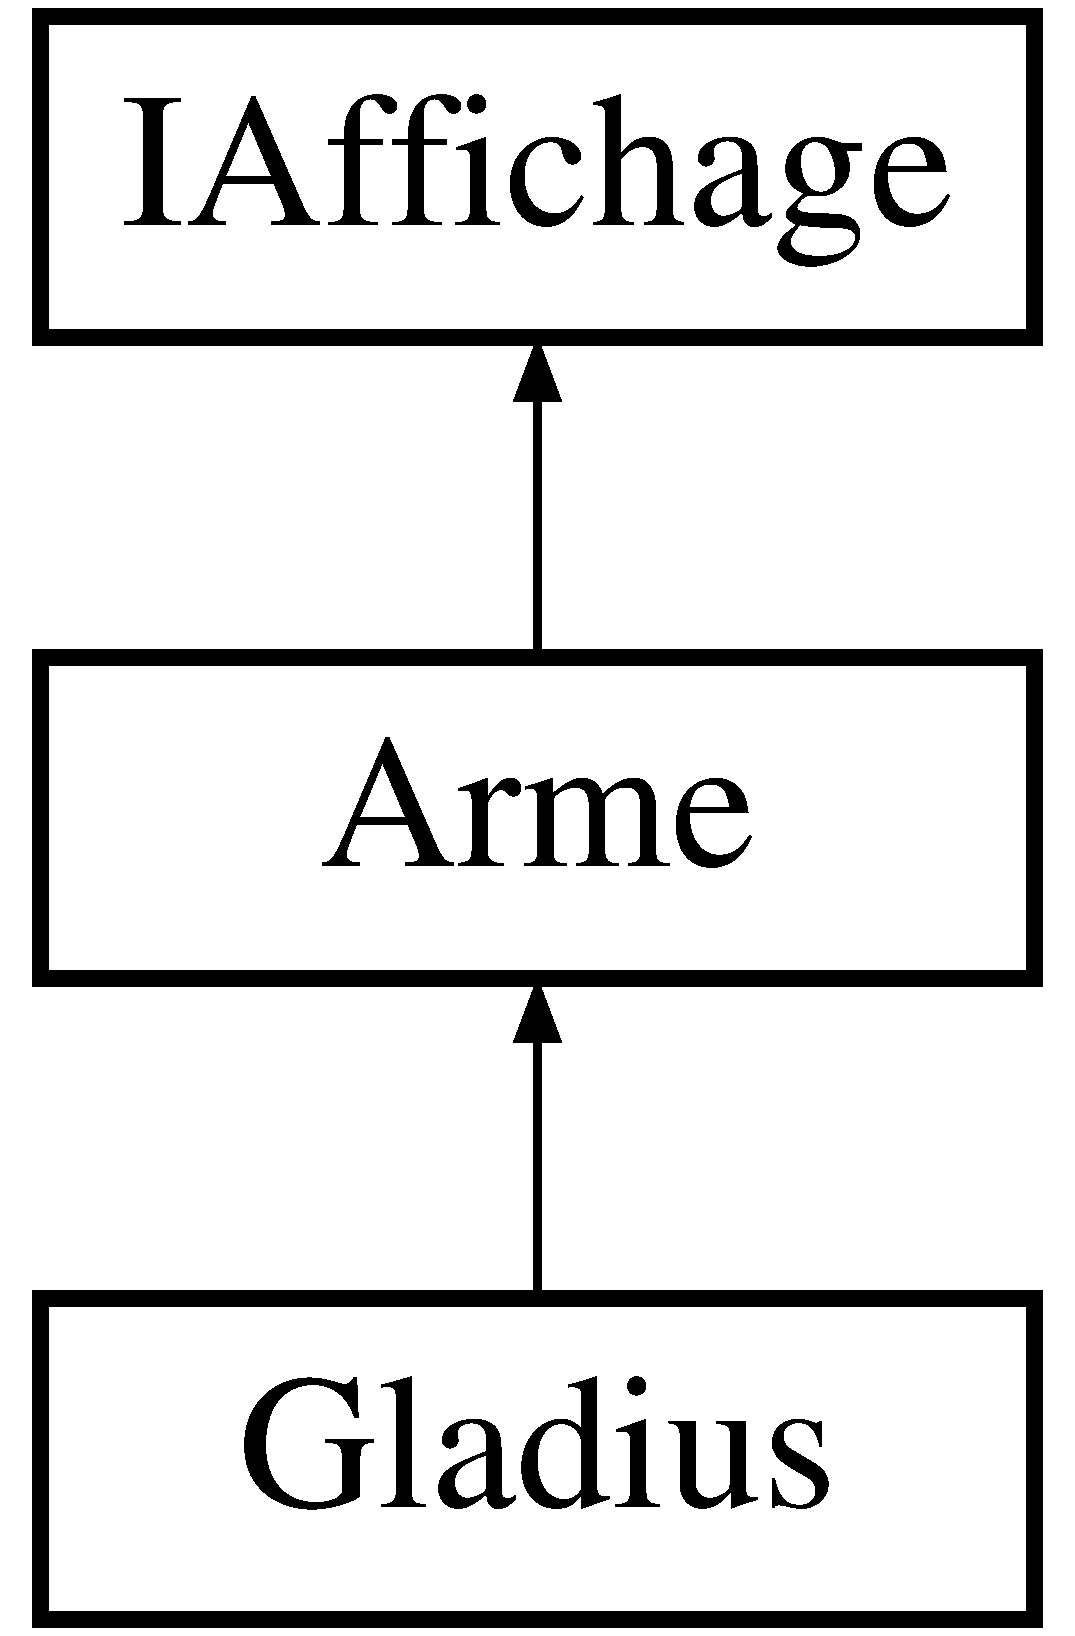
\includegraphics[height=3.000000cm]{class_gladius}
\end{center}
\end{figure}
\subsection*{\-Public \-Member \-Functions}
\begin{DoxyCompactItemize}
\item 
\hyperlink{class_gladius_aabf2b1829ee8bcefe7dcbca0361eba25}{\-Gladius} ()
\item 
int \hyperlink{class_gladius_a1eaed26d6372f759c570b77c2a623baf}{get\-Id} ()
\item 
void \hyperlink{class_gladius_a73e8bacda8c1596704be5f165422d045}{set\-Id} (int id)
\item 
string \hyperlink{class_gladius_ae303fc7e35a304fcc817ce220bf5e134}{get\-Libelle} ()
\item 
void \hyperlink{class_gladius_a42c4ac95a4bba0f81b7d7eabfef4dd40}{set\-Libelle} (string l)
\item 
int \hyperlink{class_gladius_a4b101ed656c9d27ca1c259776a6a2995}{get\-Val\-Deg} ()
\item 
void \hyperlink{class_gladius_a6edfbe46c632ebc571fa2ab5843d4373}{set\-Val\-Deg} (int v)
\end{DoxyCompactItemize}


\subsection{\-Detailed \-Description}
\-Classe \hyperlink{class_gladius}{\-Gladius}, hérite d'\hyperlink{class_arme}{\-Arme} 

\subsection{\-Constructor \& \-Destructor \-Documentation}
\hypertarget{class_gladius_aabf2b1829ee8bcefe7dcbca0361eba25}{\index{\-Gladius@{\-Gladius}!\-Gladius@{\-Gladius}}
\index{\-Gladius@{\-Gladius}!Gladius@{\-Gladius}}
\subsubsection[{\-Gladius}]{\setlength{\rightskip}{0pt plus 5cm}{\bf \-Gladius\-::\-Gladius} (
\begin{DoxyParamCaption}
{}
\end{DoxyParamCaption}
)\hspace{0.3cm}{\ttfamily  \mbox{[}inline\mbox{]}}}}\label{class_gladius_aabf2b1829ee8bcefe7dcbca0361eba25}
\-Constructeur explicite initialisant les variables du gladius 

\subsection{\-Member \-Function \-Documentation}
\hypertarget{class_gladius_a1eaed26d6372f759c570b77c2a623baf}{\index{\-Gladius@{\-Gladius}!get\-Id@{get\-Id}}
\index{get\-Id@{get\-Id}!Gladius@{\-Gladius}}
\subsubsection[{get\-Id}]{\setlength{\rightskip}{0pt plus 5cm}int {\bf \-Gladius\-::get\-Id} (
\begin{DoxyParamCaption}
{}
\end{DoxyParamCaption}
)\hspace{0.3cm}{\ttfamily  \mbox{[}inline\mbox{]}}}}\label{class_gladius_a1eaed26d6372f759c570b77c2a623baf}
\-Accesseur à l'identifiant du gladius 

\-Reimplemented from \hyperlink{class_arme_a6c957484697d9ad38ab1ed4361f3b8f4}{\-Arme}.

\hypertarget{class_gladius_ae303fc7e35a304fcc817ce220bf5e134}{\index{\-Gladius@{\-Gladius}!get\-Libelle@{get\-Libelle}}
\index{get\-Libelle@{get\-Libelle}!Gladius@{\-Gladius}}
\subsubsection[{get\-Libelle}]{\setlength{\rightskip}{0pt plus 5cm}string {\bf \-Gladius\-::get\-Libelle} (
\begin{DoxyParamCaption}
{}
\end{DoxyParamCaption}
)\hspace{0.3cm}{\ttfamily  \mbox{[}inline\mbox{]}}}}\label{class_gladius_ae303fc7e35a304fcc817ce220bf5e134}
\-Accesseur au libellé de l'arme 

\-Reimplemented from \hyperlink{class_arme_a5e43d33d0e14da19fb37dc497474135b}{\-Arme}.

\hypertarget{class_gladius_a4b101ed656c9d27ca1c259776a6a2995}{\index{\-Gladius@{\-Gladius}!get\-Val\-Deg@{get\-Val\-Deg}}
\index{get\-Val\-Deg@{get\-Val\-Deg}!Gladius@{\-Gladius}}
\subsubsection[{get\-Val\-Deg}]{\setlength{\rightskip}{0pt plus 5cm}int {\bf \-Gladius\-::get\-Val\-Deg} (
\begin{DoxyParamCaption}
{}
\end{DoxyParamCaption}
)\hspace{0.3cm}{\ttfamily  \mbox{[}inline\mbox{]}}}}\label{class_gladius_a4b101ed656c9d27ca1c259776a6a2995}
\-Accesseur à la valeur de dégâts du gladius \hypertarget{class_gladius_a73e8bacda8c1596704be5f165422d045}{\index{\-Gladius@{\-Gladius}!set\-Id@{set\-Id}}
\index{set\-Id@{set\-Id}!Gladius@{\-Gladius}}
\subsubsection[{set\-Id}]{\setlength{\rightskip}{0pt plus 5cm}void {\bf \-Gladius\-::set\-Id} (
\begin{DoxyParamCaption}
\item[{int}]{id}
\end{DoxyParamCaption}
)\hspace{0.3cm}{\ttfamily  \mbox{[}inline\mbox{]}}}}\label{class_gladius_a73e8bacda8c1596704be5f165422d045}
\-Mutateur de l'identifiant du gladius 

\-Reimplemented from \hyperlink{class_arme_a332699f4c7b2dab9e38fccfddba7275b}{\-Arme}.

\hypertarget{class_gladius_a42c4ac95a4bba0f81b7d7eabfef4dd40}{\index{\-Gladius@{\-Gladius}!set\-Libelle@{set\-Libelle}}
\index{set\-Libelle@{set\-Libelle}!Gladius@{\-Gladius}}
\subsubsection[{set\-Libelle}]{\setlength{\rightskip}{0pt plus 5cm}void {\bf \-Gladius\-::set\-Libelle} (
\begin{DoxyParamCaption}
\item[{string}]{l}
\end{DoxyParamCaption}
)\hspace{0.3cm}{\ttfamily  \mbox{[}inline\mbox{]}}}}\label{class_gladius_a42c4ac95a4bba0f81b7d7eabfef4dd40}
\-Mutateur du libellé de l'arme 

\-Reimplemented from \hyperlink{class_arme_ab38eebb032ab6773678ee40f152df6dd}{\-Arme}.

\hypertarget{class_gladius_a6edfbe46c632ebc571fa2ab5843d4373}{\index{\-Gladius@{\-Gladius}!set\-Val\-Deg@{set\-Val\-Deg}}
\index{set\-Val\-Deg@{set\-Val\-Deg}!Gladius@{\-Gladius}}
\subsubsection[{set\-Val\-Deg}]{\setlength{\rightskip}{0pt plus 5cm}void {\bf \-Gladius\-::set\-Val\-Deg} (
\begin{DoxyParamCaption}
\item[{int}]{v}
\end{DoxyParamCaption}
)\hspace{0.3cm}{\ttfamily  \mbox{[}inline\mbox{]}}}}\label{class_gladius_a6edfbe46c632ebc571fa2ab5843d4373}
\-Mutateur de la valeur de dégâts du gladius 

\-The documentation for this class was generated from the following file\-:\begin{DoxyCompactItemize}
\item 
\-Projet\-P\-O\-O-\/master/\-Gladius.\-cpp\end{DoxyCompactItemize}

\hypertarget{class_gladius_aiguise}{\section{\-Gladius\-Aiguise \-Class \-Reference}
\label{class_gladius_aiguise}\index{\-Gladius\-Aiguise@{\-Gladius\-Aiguise}}
}
\-Inheritance diagram for \-Gladius\-Aiguise\-:\begin{figure}[H]
\begin{center}
\leavevmode
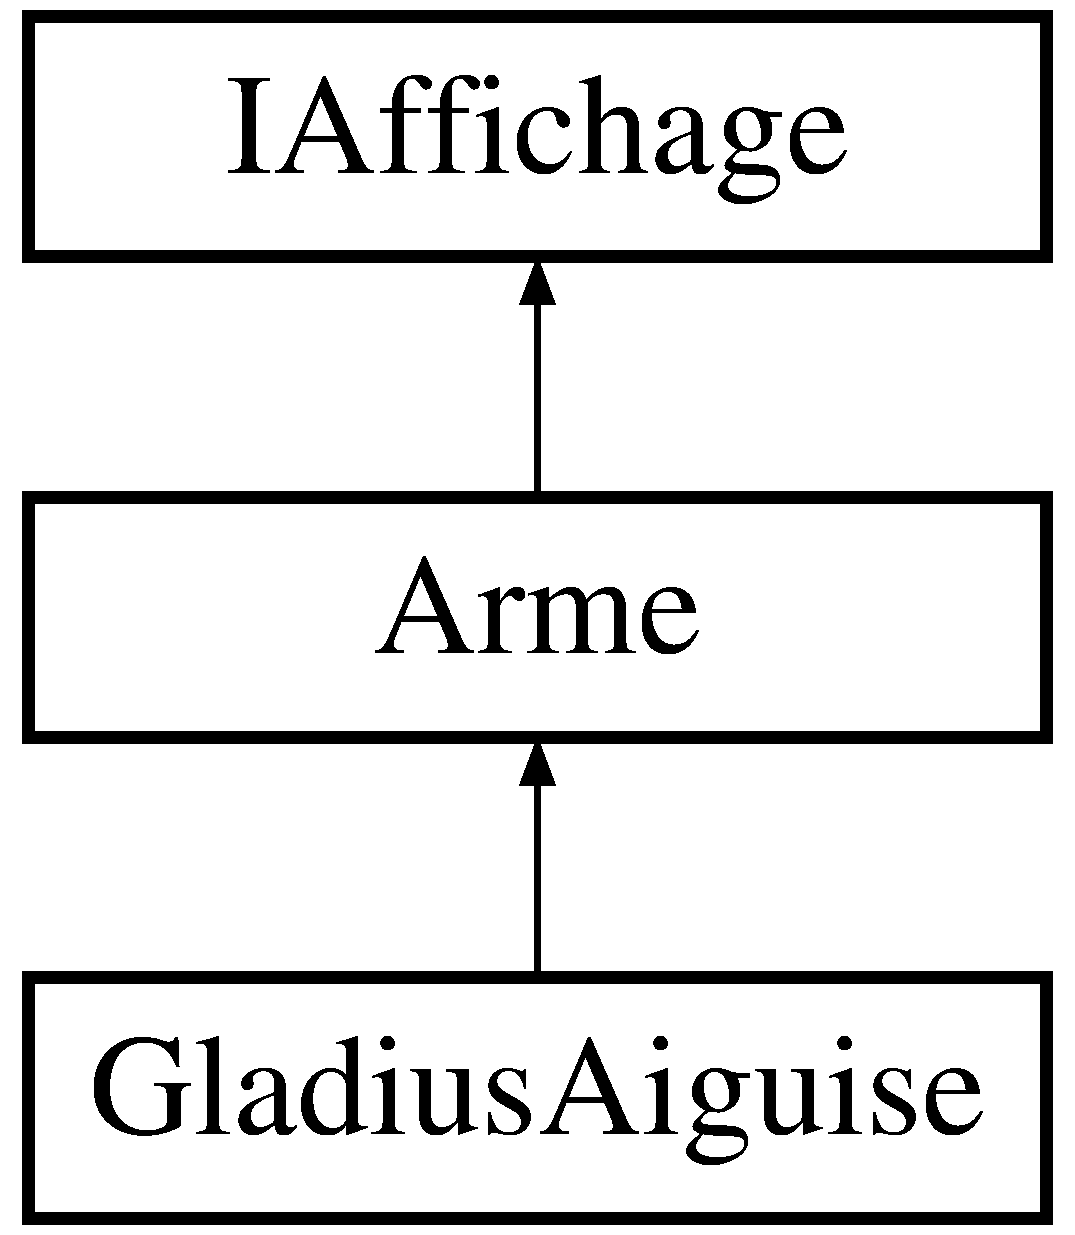
\includegraphics[height=3.000000cm]{class_gladius_aiguise}
\end{center}
\end{figure}
\subsection*{\-Public \-Member \-Functions}
\begin{DoxyCompactItemize}
\item 
int \hyperlink{class_gladius_aiguise_a9f54b9a3f9bc8bbb252dd9cc78d481d1}{get\-Id} ()
\item 
void \hyperlink{class_gladius_aiguise_a32d93fce577bca09338829bcd8544674}{set\-Id} (int id)
\item 
string \hyperlink{class_gladius_aiguise_afc73b6fd6b318112e11e6287fdbe9cff}{get\-Libelle} ()
\item 
void \hyperlink{class_gladius_aiguise_a36a9d4d8f0b92534ea50c1189be14d85}{set\-Libelle} (string l)
\item 
\hypertarget{class_gladius_aiguise_a209e41b8256153d8bef8b49a4722c4c7}{int {\bfseries get\-Val\-Deg} ()}\label{class_gladius_aiguise_a209e41b8256153d8bef8b49a4722c4c7}

\item 
\hypertarget{class_gladius_aiguise_a33bd11dcd1734857cbeec73f6642f348}{void {\bfseries set\-Val\-Deg} (int v)}\label{class_gladius_aiguise_a33bd11dcd1734857cbeec73f6642f348}

\item 
\hypertarget{class_gladius_aiguise_a01d53f6ce5a3cb94c3a4db7048454b0b}{\hyperlink{class_effet}{\-Effet} $\ast$ {\bfseries get\-Effet} ()}\label{class_gladius_aiguise_a01d53f6ce5a3cb94c3a4db7048454b0b}

\item 
\hypertarget{class_gladius_aiguise_acc1aaf2008a3cbf36ae277a055b549dd}{void {\bfseries set\-Effet} (\hyperlink{class_effet}{\-Effet} $\ast$e)}\label{class_gladius_aiguise_acc1aaf2008a3cbf36ae277a055b549dd}

\end{DoxyCompactItemize}


\subsection{\-Member \-Function \-Documentation}
\hypertarget{class_gladius_aiguise_a9f54b9a3f9bc8bbb252dd9cc78d481d1}{\index{\-Gladius\-Aiguise@{\-Gladius\-Aiguise}!get\-Id@{get\-Id}}
\index{get\-Id@{get\-Id}!GladiusAiguise@{\-Gladius\-Aiguise}}
\subsubsection[{get\-Id}]{\setlength{\rightskip}{0pt plus 5cm}int {\bf \-Gladius\-Aiguise\-::get\-Id} (
\begin{DoxyParamCaption}
{}
\end{DoxyParamCaption}
)\hspace{0.3cm}{\ttfamily  \mbox{[}inline\mbox{]}}}}\label{class_gladius_aiguise_a9f54b9a3f9bc8bbb252dd9cc78d481d1}
\-Accesseur à l'identifiant de l'arme 

\-Reimplemented from \hyperlink{class_arme_a6c957484697d9ad38ab1ed4361f3b8f4}{\-Arme}.

\hypertarget{class_gladius_aiguise_afc73b6fd6b318112e11e6287fdbe9cff}{\index{\-Gladius\-Aiguise@{\-Gladius\-Aiguise}!get\-Libelle@{get\-Libelle}}
\index{get\-Libelle@{get\-Libelle}!GladiusAiguise@{\-Gladius\-Aiguise}}
\subsubsection[{get\-Libelle}]{\setlength{\rightskip}{0pt plus 5cm}string {\bf \-Gladius\-Aiguise\-::get\-Libelle} (
\begin{DoxyParamCaption}
{}
\end{DoxyParamCaption}
)\hspace{0.3cm}{\ttfamily  \mbox{[}inline\mbox{]}}}}\label{class_gladius_aiguise_afc73b6fd6b318112e11e6287fdbe9cff}
\-Accesseur au libellé de l'arme 

\-Reimplemented from \hyperlink{class_arme_a5e43d33d0e14da19fb37dc497474135b}{\-Arme}.

\hypertarget{class_gladius_aiguise_a32d93fce577bca09338829bcd8544674}{\index{\-Gladius\-Aiguise@{\-Gladius\-Aiguise}!set\-Id@{set\-Id}}
\index{set\-Id@{set\-Id}!GladiusAiguise@{\-Gladius\-Aiguise}}
\subsubsection[{set\-Id}]{\setlength{\rightskip}{0pt plus 5cm}void {\bf \-Gladius\-Aiguise\-::set\-Id} (
\begin{DoxyParamCaption}
\item[{int}]{id}
\end{DoxyParamCaption}
)\hspace{0.3cm}{\ttfamily  \mbox{[}inline\mbox{]}}}}\label{class_gladius_aiguise_a32d93fce577bca09338829bcd8544674}
\-Mutateur de l'identifiant de l'arme 

\-Reimplemented from \hyperlink{class_arme_a332699f4c7b2dab9e38fccfddba7275b}{\-Arme}.

\hypertarget{class_gladius_aiguise_a36a9d4d8f0b92534ea50c1189be14d85}{\index{\-Gladius\-Aiguise@{\-Gladius\-Aiguise}!set\-Libelle@{set\-Libelle}}
\index{set\-Libelle@{set\-Libelle}!GladiusAiguise@{\-Gladius\-Aiguise}}
\subsubsection[{set\-Libelle}]{\setlength{\rightskip}{0pt plus 5cm}void {\bf \-Gladius\-Aiguise\-::set\-Libelle} (
\begin{DoxyParamCaption}
\item[{string}]{l}
\end{DoxyParamCaption}
)\hspace{0.3cm}{\ttfamily  \mbox{[}inline\mbox{]}}}}\label{class_gladius_aiguise_a36a9d4d8f0b92534ea50c1189be14d85}
\-Mutateur du libellé de l'arme 

\-Reimplemented from \hyperlink{class_arme_ab38eebb032ab6773678ee40f152df6dd}{\-Arme}.



\-The documentation for this class was generated from the following file\-:\begin{DoxyCompactItemize}
\item 
\-Projet\-P\-O\-O-\/master/\-Gladius\-Aiguise.\-cpp\end{DoxyCompactItemize}

\hypertarget{class_gladius_empoisonne}{\section{\-Gladius\-Empoisonne \-Class \-Reference}
\label{class_gladius_empoisonne}\index{\-Gladius\-Empoisonne@{\-Gladius\-Empoisonne}}
}
\-Inheritance diagram for \-Gladius\-Empoisonne\-:\begin{figure}[H]
\begin{center}
\leavevmode
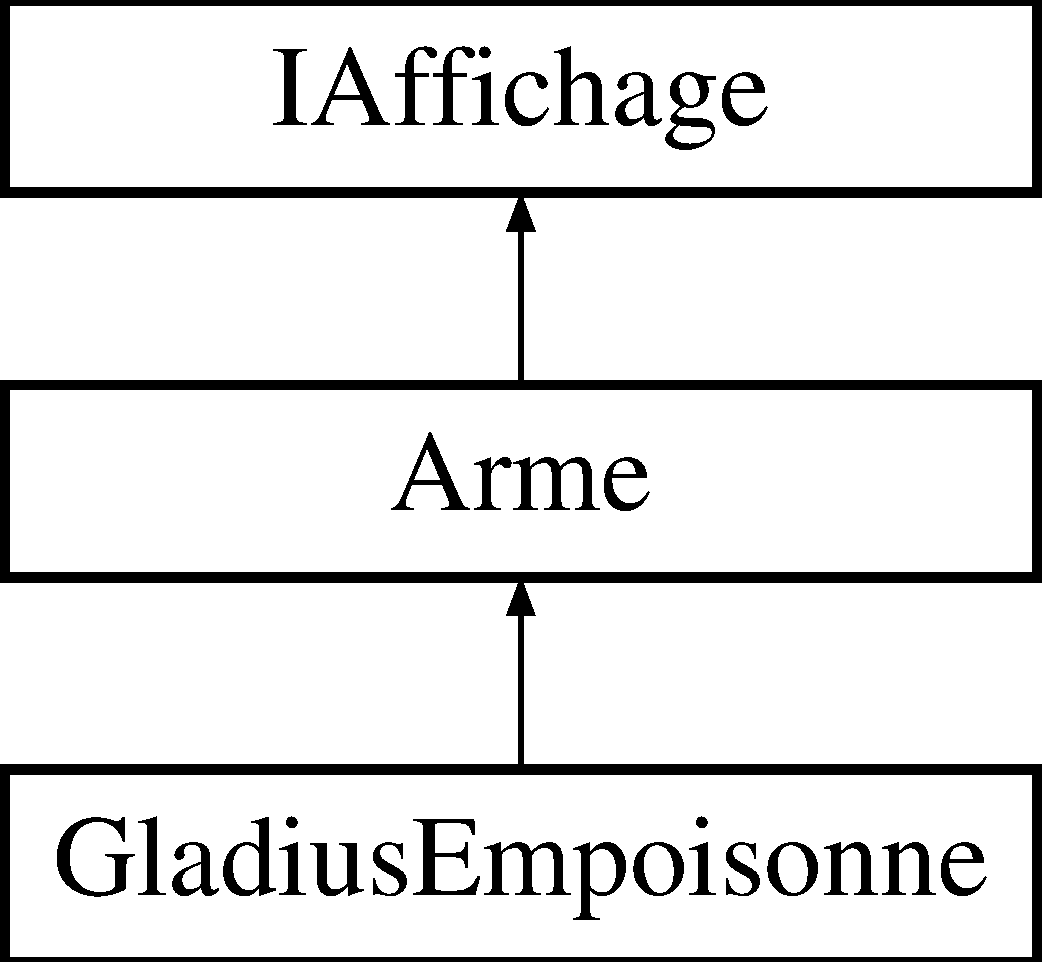
\includegraphics[height=3.000000cm]{class_gladius_empoisonne}
\end{center}
\end{figure}
\subsection*{\-Public \-Member \-Functions}
\begin{DoxyCompactItemize}
\item 
int \hyperlink{class_gladius_empoisonne_a23898d8572b5f9c552aec390cf474523}{get\-Id} ()
\item 
void \hyperlink{class_gladius_empoisonne_ac2dba19740e6b5e4c20bd2b783499682}{set\-Id} (int id)
\item 
string \hyperlink{class_gladius_empoisonne_a0db1471bda9bcd106c951ea5b1b9c7d5}{get\-Libelle} ()
\item 
void \hyperlink{class_gladius_empoisonne_af7260cdfc296aecb4433ccf9a5b18dc7}{set\-Libelle} (string l)
\item 
\hypertarget{class_gladius_empoisonne_abb1c37061e98b52d83d818c0a3c3065b}{int {\bfseries get\-Val\-Deg} ()}\label{class_gladius_empoisonne_abb1c37061e98b52d83d818c0a3c3065b}

\item 
\hypertarget{class_gladius_empoisonne_ab32eae0eafd4b365df10729b2a50367d}{void {\bfseries set\-Val\-Deg} (int v)}\label{class_gladius_empoisonne_ab32eae0eafd4b365df10729b2a50367d}

\item 
\hypertarget{class_gladius_empoisonne_af97519c3f19397455f0cf9eaa76b886d}{\hyperlink{class_effet}{\-Effet} $\ast$ {\bfseries get\-Effet} ()}\label{class_gladius_empoisonne_af97519c3f19397455f0cf9eaa76b886d}

\item 
\hypertarget{class_gladius_empoisonne_ab238f4b62f0ee6fa114db5167428dd3a}{void {\bfseries set\-Effet} (\hyperlink{class_effet}{\-Effet} $\ast$e)}\label{class_gladius_empoisonne_ab238f4b62f0ee6fa114db5167428dd3a}

\end{DoxyCompactItemize}


\subsection{\-Member \-Function \-Documentation}
\hypertarget{class_gladius_empoisonne_a23898d8572b5f9c552aec390cf474523}{\index{\-Gladius\-Empoisonne@{\-Gladius\-Empoisonne}!get\-Id@{get\-Id}}
\index{get\-Id@{get\-Id}!GladiusEmpoisonne@{\-Gladius\-Empoisonne}}
\subsubsection[{get\-Id}]{\setlength{\rightskip}{0pt plus 5cm}int {\bf \-Gladius\-Empoisonne\-::get\-Id} (
\begin{DoxyParamCaption}
{}
\end{DoxyParamCaption}
)\hspace{0.3cm}{\ttfamily  \mbox{[}inline\mbox{]}}}}\label{class_gladius_empoisonne_a23898d8572b5f9c552aec390cf474523}
\-Accesseur à l'identifiant de l'arme 

\-Reimplemented from \hyperlink{class_arme_a6c957484697d9ad38ab1ed4361f3b8f4}{\-Arme}.

\hypertarget{class_gladius_empoisonne_a0db1471bda9bcd106c951ea5b1b9c7d5}{\index{\-Gladius\-Empoisonne@{\-Gladius\-Empoisonne}!get\-Libelle@{get\-Libelle}}
\index{get\-Libelle@{get\-Libelle}!GladiusEmpoisonne@{\-Gladius\-Empoisonne}}
\subsubsection[{get\-Libelle}]{\setlength{\rightskip}{0pt plus 5cm}string {\bf \-Gladius\-Empoisonne\-::get\-Libelle} (
\begin{DoxyParamCaption}
{}
\end{DoxyParamCaption}
)\hspace{0.3cm}{\ttfamily  \mbox{[}inline\mbox{]}}}}\label{class_gladius_empoisonne_a0db1471bda9bcd106c951ea5b1b9c7d5}
\-Accesseur au libellé de l'arme 

\-Reimplemented from \hyperlink{class_arme_a5e43d33d0e14da19fb37dc497474135b}{\-Arme}.

\hypertarget{class_gladius_empoisonne_ac2dba19740e6b5e4c20bd2b783499682}{\index{\-Gladius\-Empoisonne@{\-Gladius\-Empoisonne}!set\-Id@{set\-Id}}
\index{set\-Id@{set\-Id}!GladiusEmpoisonne@{\-Gladius\-Empoisonne}}
\subsubsection[{set\-Id}]{\setlength{\rightskip}{0pt plus 5cm}void {\bf \-Gladius\-Empoisonne\-::set\-Id} (
\begin{DoxyParamCaption}
\item[{int}]{id}
\end{DoxyParamCaption}
)\hspace{0.3cm}{\ttfamily  \mbox{[}inline\mbox{]}}}}\label{class_gladius_empoisonne_ac2dba19740e6b5e4c20bd2b783499682}
\-Mutateur de l'identifiant de l'arme 

\-Reimplemented from \hyperlink{class_arme_a332699f4c7b2dab9e38fccfddba7275b}{\-Arme}.

\hypertarget{class_gladius_empoisonne_af7260cdfc296aecb4433ccf9a5b18dc7}{\index{\-Gladius\-Empoisonne@{\-Gladius\-Empoisonne}!set\-Libelle@{set\-Libelle}}
\index{set\-Libelle@{set\-Libelle}!GladiusEmpoisonne@{\-Gladius\-Empoisonne}}
\subsubsection[{set\-Libelle}]{\setlength{\rightskip}{0pt plus 5cm}void {\bf \-Gladius\-Empoisonne\-::set\-Libelle} (
\begin{DoxyParamCaption}
\item[{string}]{l}
\end{DoxyParamCaption}
)\hspace{0.3cm}{\ttfamily  \mbox{[}inline\mbox{]}}}}\label{class_gladius_empoisonne_af7260cdfc296aecb4433ccf9a5b18dc7}
\-Mutateur du libellé de l'arme 

\-Reimplemented from \hyperlink{class_arme_ab38eebb032ab6773678ee40f152df6dd}{\-Arme}.



\-The documentation for this class was generated from the following file\-:\begin{DoxyCompactItemize}
\item 
\-Projet\-P\-O\-O-\/master/\-Gladius\-Empoisonne.\-cpp\end{DoxyCompactItemize}

\hypertarget{class_greve}{\section{\-Greve \-Class \-Reference}
\label{class_greve}\index{\-Greve@{\-Greve}}
}
\-Inheritance diagram for \-Greve\-:\begin{figure}[H]
\begin{center}
\leavevmode
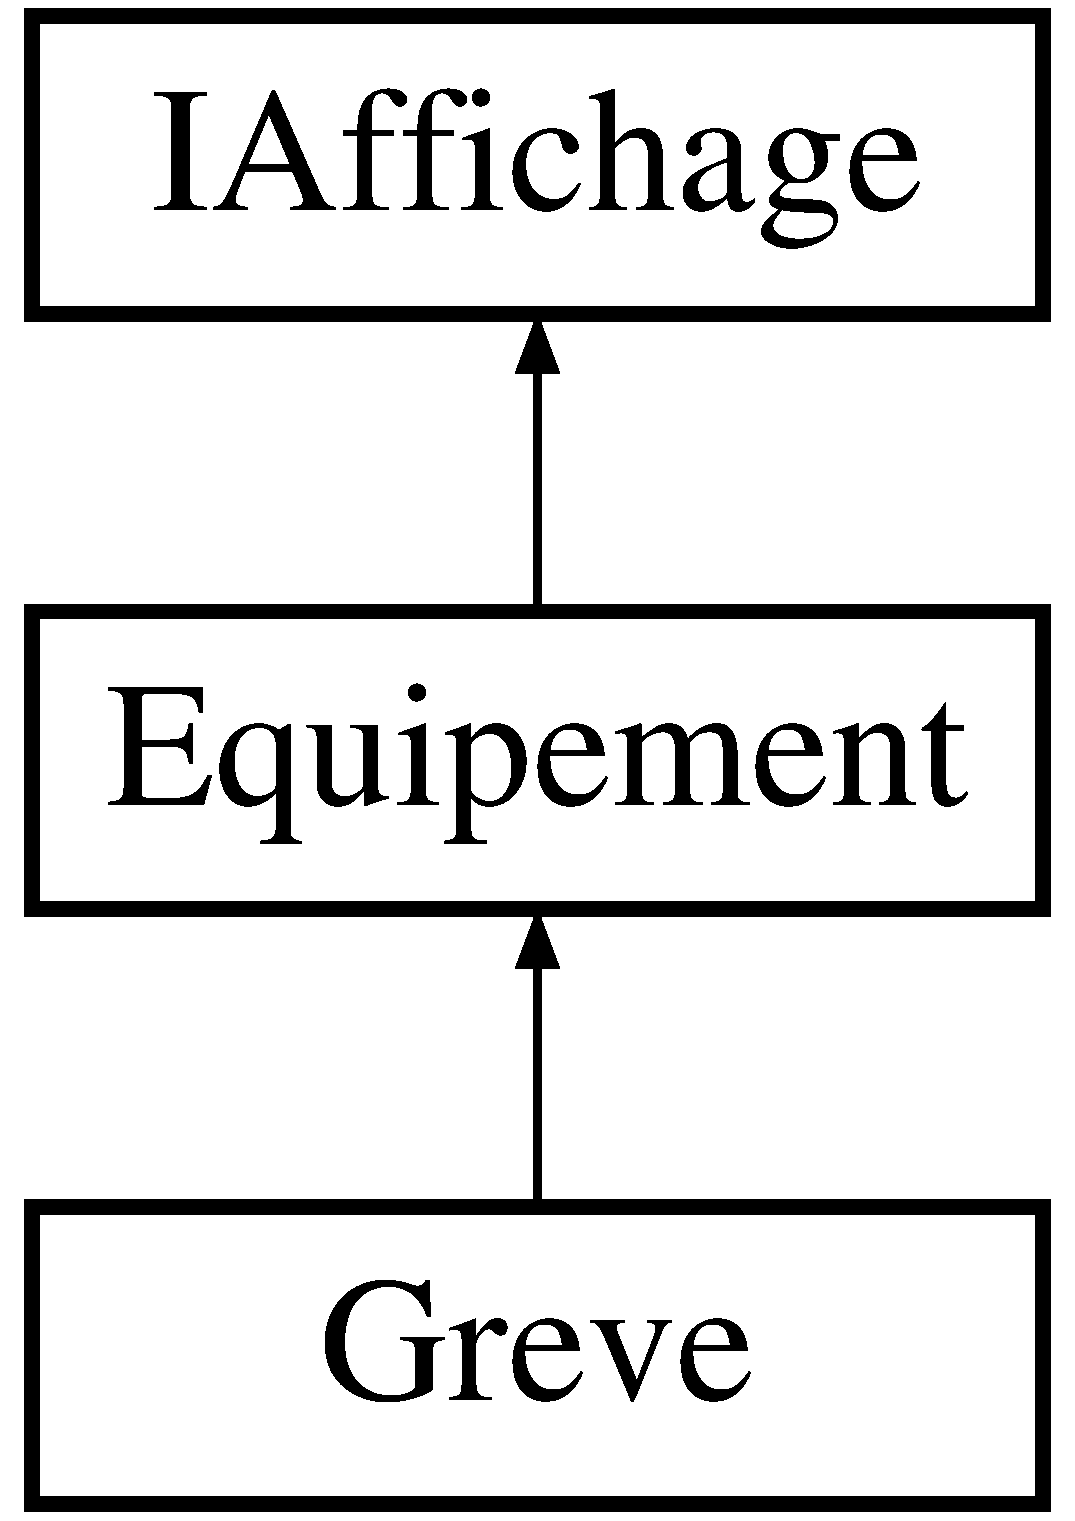
\includegraphics[height=3.000000cm]{class_greve}
\end{center}
\end{figure}
\subsection*{\-Public \-Member \-Functions}
\begin{DoxyCompactItemize}
\item 
\hyperlink{class_greve_a49a67ac38e5962e21f3718eb8dac35ac}{\-Greve} ()
\item 
int \hyperlink{class_greve_a9d1f9157ba388f329a51ba447950c257}{get\-Id} ()
\item 
void \hyperlink{class_greve_ac940e6600c26f1b0d2ecfd9d9dd5cbea}{set\-Id} (int id)
\item 
string \hyperlink{class_greve_a11a9352790169fab9893ce8ef96f657c}{get\-Libelle} ()
\item 
void \hyperlink{class_greve_ab1cc65d30d2e6531ee1904449f812e14}{set\-Libelle} (string l)
\item 
int \hyperlink{class_greve_ad03dddd443d2452134827983aa3541ec}{get\-Val\-Def} ()
\item 
void \hyperlink{class_greve_ab5cabb1d422d0af2d15f733ecbe3af41}{set\-Val\-Def} (int v)
\end{DoxyCompactItemize}


\subsection{\-Detailed \-Description}
\-Classe \hyperlink{class_greve}{\-Greve}, hérite d'\hyperlink{class_equipement}{\-Equipement} 

\subsection{\-Constructor \& \-Destructor \-Documentation}
\hypertarget{class_greve_a49a67ac38e5962e21f3718eb8dac35ac}{\index{\-Greve@{\-Greve}!\-Greve@{\-Greve}}
\index{\-Greve@{\-Greve}!Greve@{\-Greve}}
\subsubsection[{\-Greve}]{\setlength{\rightskip}{0pt plus 5cm}{\bf \-Greve\-::\-Greve} (
\begin{DoxyParamCaption}
{}
\end{DoxyParamCaption}
)\hspace{0.3cm}{\ttfamily  \mbox{[}inline\mbox{]}}}}\label{class_greve_a49a67ac38e5962e21f3718eb8dac35ac}
\-Constructeur explicite initialisant les variables de la grève 

\subsection{\-Member \-Function \-Documentation}
\hypertarget{class_greve_a9d1f9157ba388f329a51ba447950c257}{\index{\-Greve@{\-Greve}!get\-Id@{get\-Id}}
\index{get\-Id@{get\-Id}!Greve@{\-Greve}}
\subsubsection[{get\-Id}]{\setlength{\rightskip}{0pt plus 5cm}int {\bf \-Greve\-::get\-Id} (
\begin{DoxyParamCaption}
{}
\end{DoxyParamCaption}
)\hspace{0.3cm}{\ttfamily  \mbox{[}inline\mbox{]}}}}\label{class_greve_a9d1f9157ba388f329a51ba447950c257}
\-Accesseur à l'identifiant de la grève 

\-Reimplemented from \hyperlink{class_equipement_abc38941f5a9deed943b7a83ce69539c3}{\-Equipement}.

\hypertarget{class_greve_a11a9352790169fab9893ce8ef96f657c}{\index{\-Greve@{\-Greve}!get\-Libelle@{get\-Libelle}}
\index{get\-Libelle@{get\-Libelle}!Greve@{\-Greve}}
\subsubsection[{get\-Libelle}]{\setlength{\rightskip}{0pt plus 5cm}string {\bf \-Greve\-::get\-Libelle} (
\begin{DoxyParamCaption}
{}
\end{DoxyParamCaption}
)\hspace{0.3cm}{\ttfamily  \mbox{[}inline\mbox{]}}}}\label{class_greve_a11a9352790169fab9893ce8ef96f657c}
\-Accesseur au libellé de l'équipement 

\-Reimplemented from \hyperlink{class_equipement_ab00ec565966647bf6edeb1a9df430aa6}{\-Equipement}.

\hypertarget{class_greve_ad03dddd443d2452134827983aa3541ec}{\index{\-Greve@{\-Greve}!get\-Val\-Def@{get\-Val\-Def}}
\index{get\-Val\-Def@{get\-Val\-Def}!Greve@{\-Greve}}
\subsubsection[{get\-Val\-Def}]{\setlength{\rightskip}{0pt plus 5cm}int {\bf \-Greve\-::get\-Val\-Def} (
\begin{DoxyParamCaption}
{}
\end{DoxyParamCaption}
)\hspace{0.3cm}{\ttfamily  \mbox{[}inline\mbox{]}}}}\label{class_greve_ad03dddd443d2452134827983aa3541ec}
\-Accesseur à la valeur de défense de la grève 

\-Reimplemented from \hyperlink{class_equipement_a7b3003f4da24a94bfec94555e35e772c}{\-Equipement}.

\hypertarget{class_greve_ac940e6600c26f1b0d2ecfd9d9dd5cbea}{\index{\-Greve@{\-Greve}!set\-Id@{set\-Id}}
\index{set\-Id@{set\-Id}!Greve@{\-Greve}}
\subsubsection[{set\-Id}]{\setlength{\rightskip}{0pt plus 5cm}void {\bf \-Greve\-::set\-Id} (
\begin{DoxyParamCaption}
\item[{int}]{id}
\end{DoxyParamCaption}
)\hspace{0.3cm}{\ttfamily  \mbox{[}inline\mbox{]}}}}\label{class_greve_ac940e6600c26f1b0d2ecfd9d9dd5cbea}
\-Mutateur de l'identifiant de la grève 

\-Reimplemented from \hyperlink{class_equipement_a98208826ad05cbc38211e9f70bd908c5}{\-Equipement}.

\hypertarget{class_greve_ab1cc65d30d2e6531ee1904449f812e14}{\index{\-Greve@{\-Greve}!set\-Libelle@{set\-Libelle}}
\index{set\-Libelle@{set\-Libelle}!Greve@{\-Greve}}
\subsubsection[{set\-Libelle}]{\setlength{\rightskip}{0pt plus 5cm}void {\bf \-Greve\-::set\-Libelle} (
\begin{DoxyParamCaption}
\item[{string}]{l}
\end{DoxyParamCaption}
)\hspace{0.3cm}{\ttfamily  \mbox{[}inline\mbox{]}}}}\label{class_greve_ab1cc65d30d2e6531ee1904449f812e14}
\-Mutateur du libellé de l'équipement 

\-Reimplemented from \hyperlink{class_equipement_aea246b68c747bd5ec84ca8ce4c4c7b40}{\-Equipement}.

\hypertarget{class_greve_ab5cabb1d422d0af2d15f733ecbe3af41}{\index{\-Greve@{\-Greve}!set\-Val\-Def@{set\-Val\-Def}}
\index{set\-Val\-Def@{set\-Val\-Def}!Greve@{\-Greve}}
\subsubsection[{set\-Val\-Def}]{\setlength{\rightskip}{0pt plus 5cm}void {\bf \-Greve\-::set\-Val\-Def} (
\begin{DoxyParamCaption}
\item[{int}]{v}
\end{DoxyParamCaption}
)\hspace{0.3cm}{\ttfamily  \mbox{[}inline\mbox{]}}}}\label{class_greve_ab5cabb1d422d0af2d15f733ecbe3af41}
\-Mutateur de la valeur de défense de la grève 

\-Reimplemented from \hyperlink{class_equipement_ad9940c901b3a96b91c5c3f24713face5}{\-Equipement}.



\-The documentation for this class was generated from the following file\-:\begin{DoxyCompactItemize}
\item 
\-Projet\-P\-O\-O-\/master/\-Greve.\-cpp\end{DoxyCompactItemize}

\hypertarget{class_i_affichage}{\section{\-I\-Affichage \-Class \-Reference}
\label{class_i_affichage}\index{\-I\-Affichage@{\-I\-Affichage}}
}


{\ttfamily \#include $<$\-I\-Affichage.\-hpp$>$}

\-Inheritance diagram for \-I\-Affichage\-:\begin{figure}[H]
\begin{center}
\leavevmode
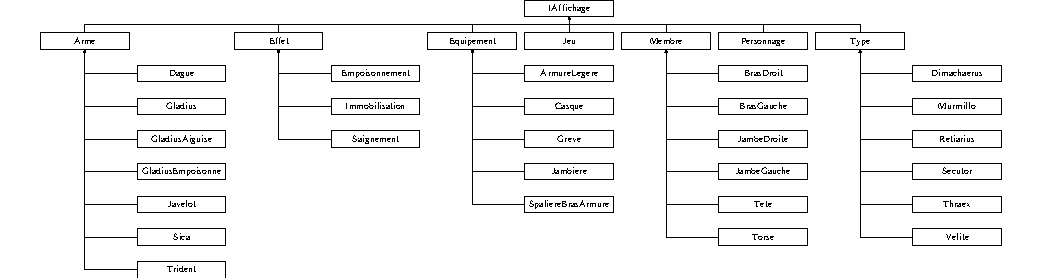
\includegraphics[height=3.733333cm]{class_i_affichage}
\end{center}
\end{figure}
\subsection*{\-Public \-Member \-Functions}
\begin{DoxyCompactItemize}
\item 
virtual \hyperlink{class_i_affichage_ae61f86e1d0cd2d54630ed16fd160b041}{$\sim$\-I\-Affichage} ()
\item 
virtual void \hyperlink{class_i_affichage_a6123c1cb9079f712b48c0b8bf62e14ef}{afficher\-Info} ()=0
\end{DoxyCompactItemize}


\subsection{\-Detailed \-Description}
\-Interface d'affichage implémentée par toutes les classes de l'application 

\subsection{\-Constructor \& \-Destructor \-Documentation}
\hypertarget{class_i_affichage_ae61f86e1d0cd2d54630ed16fd160b041}{\index{\-I\-Affichage@{\-I\-Affichage}!$\sim$\-I\-Affichage@{$\sim$\-I\-Affichage}}
\index{$\sim$\-I\-Affichage@{$\sim$\-I\-Affichage}!IAffichage@{\-I\-Affichage}}
\subsubsection[{$\sim$\-I\-Affichage}]{\setlength{\rightskip}{0pt plus 5cm}virtual {\bf \-I\-Affichage\-::$\sim$\-I\-Affichage} (
\begin{DoxyParamCaption}
{}
\end{DoxyParamCaption}
)\hspace{0.3cm}{\ttfamily  \mbox{[}inline, virtual\mbox{]}}}}\label{class_i_affichage_ae61f86e1d0cd2d54630ed16fd160b041}
\-Destructeur explicite 

\subsection{\-Member \-Function \-Documentation}
\hypertarget{class_i_affichage_a6123c1cb9079f712b48c0b8bf62e14ef}{\index{\-I\-Affichage@{\-I\-Affichage}!afficher\-Info@{afficher\-Info}}
\index{afficher\-Info@{afficher\-Info}!IAffichage@{\-I\-Affichage}}
\subsubsection[{afficher\-Info}]{\setlength{\rightskip}{0pt plus 5cm}virtual void {\bf \-I\-Affichage\-::afficher\-Info} (
\begin{DoxyParamCaption}
{}
\end{DoxyParamCaption}
)\hspace{0.3cm}{\ttfamily  \mbox{[}pure virtual\mbox{]}}}}\label{class_i_affichage_a6123c1cb9079f712b48c0b8bf62e14ef}
\-Méthode d'affichage à redéfinir par chaque classe utilisatrice 

\-Implemented in \hyperlink{class_personnage_a79ce4d8f13bc64471c553a32f2bb0e2d}{\-Personnage}, \hyperlink{class_jeu_a40747c204660ad830d76378d0cbac1f0}{\-Jeu}, \hyperlink{class_membre_adc88d8e745a6a46a90722ea2397598c9}{\-Membre}, \hyperlink{class_effet_afa8ada372b122c1447ee6ac51b551f6a}{\-Effet}, \hyperlink{class_equipement_a8db0d237091051e004df0e2274e9e015}{\-Equipement}, \hyperlink{class_arme_ac815d060b7652e01e6813656d0880b20}{\-Arme}, and \hyperlink{class_type_a793d8cc8a1e9a491803a3e9331e0ddc6}{\-Type}.



\-The documentation for this class was generated from the following file\-:\begin{DoxyCompactItemize}
\item 
\-Projet\-P\-O\-O-\/master/\-I\-Affichage.\-hpp\end{DoxyCompactItemize}

\hypertarget{class_immobilisation}{\section{\-Immobilisation \-Class \-Reference}
\label{class_immobilisation}\index{\-Immobilisation@{\-Immobilisation}}
}
\-Inheritance diagram for \-Immobilisation\-:\begin{figure}[H]
\begin{center}
\leavevmode
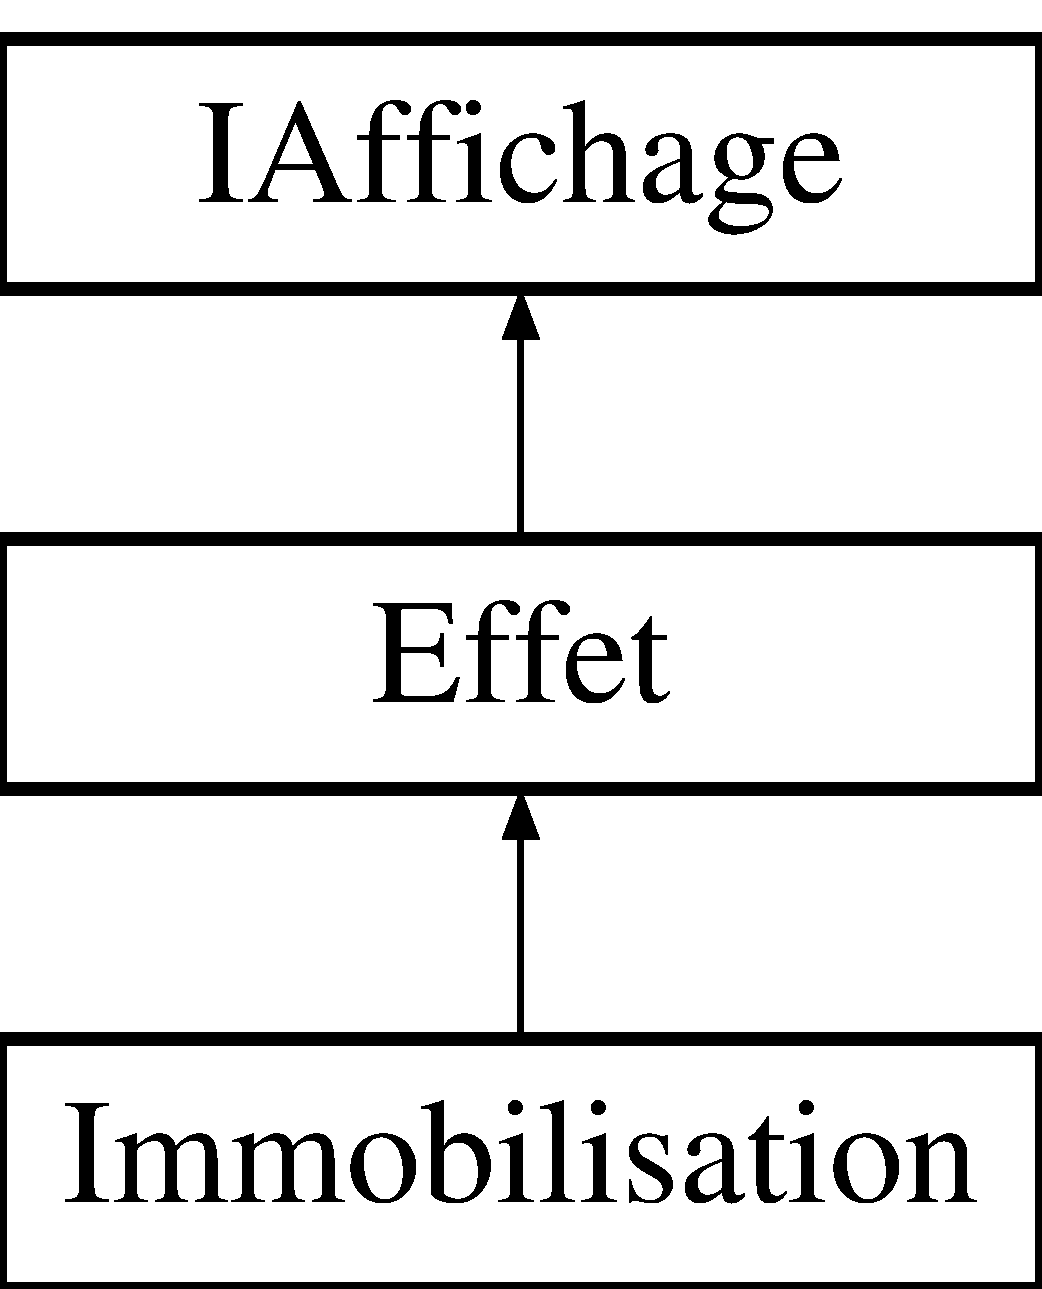
\includegraphics[height=3.000000cm]{class_immobilisation}
\end{center}
\end{figure}
\subsection*{\-Public \-Member \-Functions}
\begin{DoxyCompactItemize}
\item 
\hyperlink{class_immobilisation_a87ac7ebcbabd1cadc063254aec060958}{\-Immobilisation} ()
\item 
int \hyperlink{class_immobilisation_a4ffaa8356838b9bc202e16136bed7c93}{get\-Id} ()
\item 
void \hyperlink{class_immobilisation_a1b0d3098ec798b0c8d46ff51aa0c0db2}{set\-Id} (int id)
\item 
string \hyperlink{class_immobilisation_a77ed10535746670f2e0cdfcf385884a2}{get\-Libelle} ()
\item 
void \hyperlink{class_immobilisation_a32e8e9379388f0a492fe0fd97ec9c304}{set\-Libelle} (string l)
\item 
int \hyperlink{class_immobilisation_ae0baa3a4c8e7e39ba0646c5afda69ce8}{get\-Nb\-Tours\-Max} ()
\item 
void \hyperlink{class_immobilisation_a2b4a2b1ee2ef7b0e11ca3cf92ec4caad}{set\-Nb\-Tours\-Max} (int n)
\end{DoxyCompactItemize}


\subsection{\-Detailed \-Description}
\-Classe \hyperlink{class_immobilisation}{\-Immobilisation}, hérite d'\hyperlink{class_effet}{\-Effet} 

\subsection{\-Constructor \& \-Destructor \-Documentation}
\hypertarget{class_immobilisation_a87ac7ebcbabd1cadc063254aec060958}{\index{\-Immobilisation@{\-Immobilisation}!\-Immobilisation@{\-Immobilisation}}
\index{\-Immobilisation@{\-Immobilisation}!Immobilisation@{\-Immobilisation}}
\subsubsection[{\-Immobilisation}]{\setlength{\rightskip}{0pt plus 5cm}{\bf \-Immobilisation\-::\-Immobilisation} (
\begin{DoxyParamCaption}
{}
\end{DoxyParamCaption}
)\hspace{0.3cm}{\ttfamily  \mbox{[}inline\mbox{]}}}}\label{class_immobilisation_a87ac7ebcbabd1cadc063254aec060958}
\-Constructeur explicite initialisant les variables de l'effet 

\subsection{\-Member \-Function \-Documentation}
\hypertarget{class_immobilisation_a4ffaa8356838b9bc202e16136bed7c93}{\index{\-Immobilisation@{\-Immobilisation}!get\-Id@{get\-Id}}
\index{get\-Id@{get\-Id}!Immobilisation@{\-Immobilisation}}
\subsubsection[{get\-Id}]{\setlength{\rightskip}{0pt plus 5cm}int {\bf \-Immobilisation\-::get\-Id} (
\begin{DoxyParamCaption}
{}
\end{DoxyParamCaption}
)\hspace{0.3cm}{\ttfamily  \mbox{[}inline\mbox{]}}}}\label{class_immobilisation_a4ffaa8356838b9bc202e16136bed7c93}
\-Accesseur à l'identifiant de l'effet 

\-Reimplemented from \hyperlink{class_effet_a509c2d845776b583280b4418585d9ec2}{\-Effet}.

\hypertarget{class_immobilisation_a77ed10535746670f2e0cdfcf385884a2}{\index{\-Immobilisation@{\-Immobilisation}!get\-Libelle@{get\-Libelle}}
\index{get\-Libelle@{get\-Libelle}!Immobilisation@{\-Immobilisation}}
\subsubsection[{get\-Libelle}]{\setlength{\rightskip}{0pt plus 5cm}string {\bf \-Immobilisation\-::get\-Libelle} (
\begin{DoxyParamCaption}
{}
\end{DoxyParamCaption}
)\hspace{0.3cm}{\ttfamily  \mbox{[}inline\mbox{]}}}}\label{class_immobilisation_a77ed10535746670f2e0cdfcf385884a2}
\-Accesseur au libellé de l'effet 

\-Reimplemented from \hyperlink{class_effet_a1817f59e4c17c91103ae4031868dfd97}{\-Effet}.

\hypertarget{class_immobilisation_ae0baa3a4c8e7e39ba0646c5afda69ce8}{\index{\-Immobilisation@{\-Immobilisation}!get\-Nb\-Tours\-Max@{get\-Nb\-Tours\-Max}}
\index{get\-Nb\-Tours\-Max@{get\-Nb\-Tours\-Max}!Immobilisation@{\-Immobilisation}}
\subsubsection[{get\-Nb\-Tours\-Max}]{\setlength{\rightskip}{0pt plus 5cm}int {\bf \-Immobilisation\-::get\-Nb\-Tours\-Max} (
\begin{DoxyParamCaption}
{}
\end{DoxyParamCaption}
)\hspace{0.3cm}{\ttfamily  \mbox{[}inline\mbox{]}}}}\label{class_immobilisation_ae0baa3a4c8e7e39ba0646c5afda69ce8}
\-Accesseur à la durée maximale, en tours, de l'effet 

\-Reimplemented from \hyperlink{class_effet_ae98c2a33fcd29629e3c7cd6e8ab8fcd8}{\-Effet}.

\hypertarget{class_immobilisation_a1b0d3098ec798b0c8d46ff51aa0c0db2}{\index{\-Immobilisation@{\-Immobilisation}!set\-Id@{set\-Id}}
\index{set\-Id@{set\-Id}!Immobilisation@{\-Immobilisation}}
\subsubsection[{set\-Id}]{\setlength{\rightskip}{0pt plus 5cm}void {\bf \-Immobilisation\-::set\-Id} (
\begin{DoxyParamCaption}
\item[{int}]{id}
\end{DoxyParamCaption}
)\hspace{0.3cm}{\ttfamily  \mbox{[}inline\mbox{]}}}}\label{class_immobilisation_a1b0d3098ec798b0c8d46ff51aa0c0db2}
\-Mutateur de l'identifiant de l'effet 

\-Reimplemented from \hyperlink{class_effet_a1e880a5364a175e90dae7cbfdc103e02}{\-Effet}.

\hypertarget{class_immobilisation_a32e8e9379388f0a492fe0fd97ec9c304}{\index{\-Immobilisation@{\-Immobilisation}!set\-Libelle@{set\-Libelle}}
\index{set\-Libelle@{set\-Libelle}!Immobilisation@{\-Immobilisation}}
\subsubsection[{set\-Libelle}]{\setlength{\rightskip}{0pt plus 5cm}void {\bf \-Immobilisation\-::set\-Libelle} (
\begin{DoxyParamCaption}
\item[{string}]{l}
\end{DoxyParamCaption}
)\hspace{0.3cm}{\ttfamily  \mbox{[}inline\mbox{]}}}}\label{class_immobilisation_a32e8e9379388f0a492fe0fd97ec9c304}
\-Mutateur du libellé de l'effet 

\-Reimplemented from \hyperlink{class_effet_a8470c57c7d69b4023c5230cdca79631d}{\-Effet}.

\hypertarget{class_immobilisation_a2b4a2b1ee2ef7b0e11ca3cf92ec4caad}{\index{\-Immobilisation@{\-Immobilisation}!set\-Nb\-Tours\-Max@{set\-Nb\-Tours\-Max}}
\index{set\-Nb\-Tours\-Max@{set\-Nb\-Tours\-Max}!Immobilisation@{\-Immobilisation}}
\subsubsection[{set\-Nb\-Tours\-Max}]{\setlength{\rightskip}{0pt plus 5cm}void {\bf \-Immobilisation\-::set\-Nb\-Tours\-Max} (
\begin{DoxyParamCaption}
\item[{int}]{n}
\end{DoxyParamCaption}
)\hspace{0.3cm}{\ttfamily  \mbox{[}inline\mbox{]}}}}\label{class_immobilisation_a2b4a2b1ee2ef7b0e11ca3cf92ec4caad}
\-Mutateur de la durée maximale, en tours, de l'effet 

\-Reimplemented from \hyperlink{class_effet_a12959d98a93ca835aedd8b7ed84e5a61}{\-Effet}.



\-The documentation for this class was generated from the following file\-:\begin{DoxyCompactItemize}
\item 
\-Projet\-P\-O\-O-\/master/\-Immobilisation.\-cpp\end{DoxyCompactItemize}

\hypertarget{class_jambe_droite}{\section{\-Jambe\-Droite \-Class \-Reference}
\label{class_jambe_droite}\index{\-Jambe\-Droite@{\-Jambe\-Droite}}
}
\-Inheritance diagram for \-Jambe\-Droite\-:\begin{figure}[H]
\begin{center}
\leavevmode
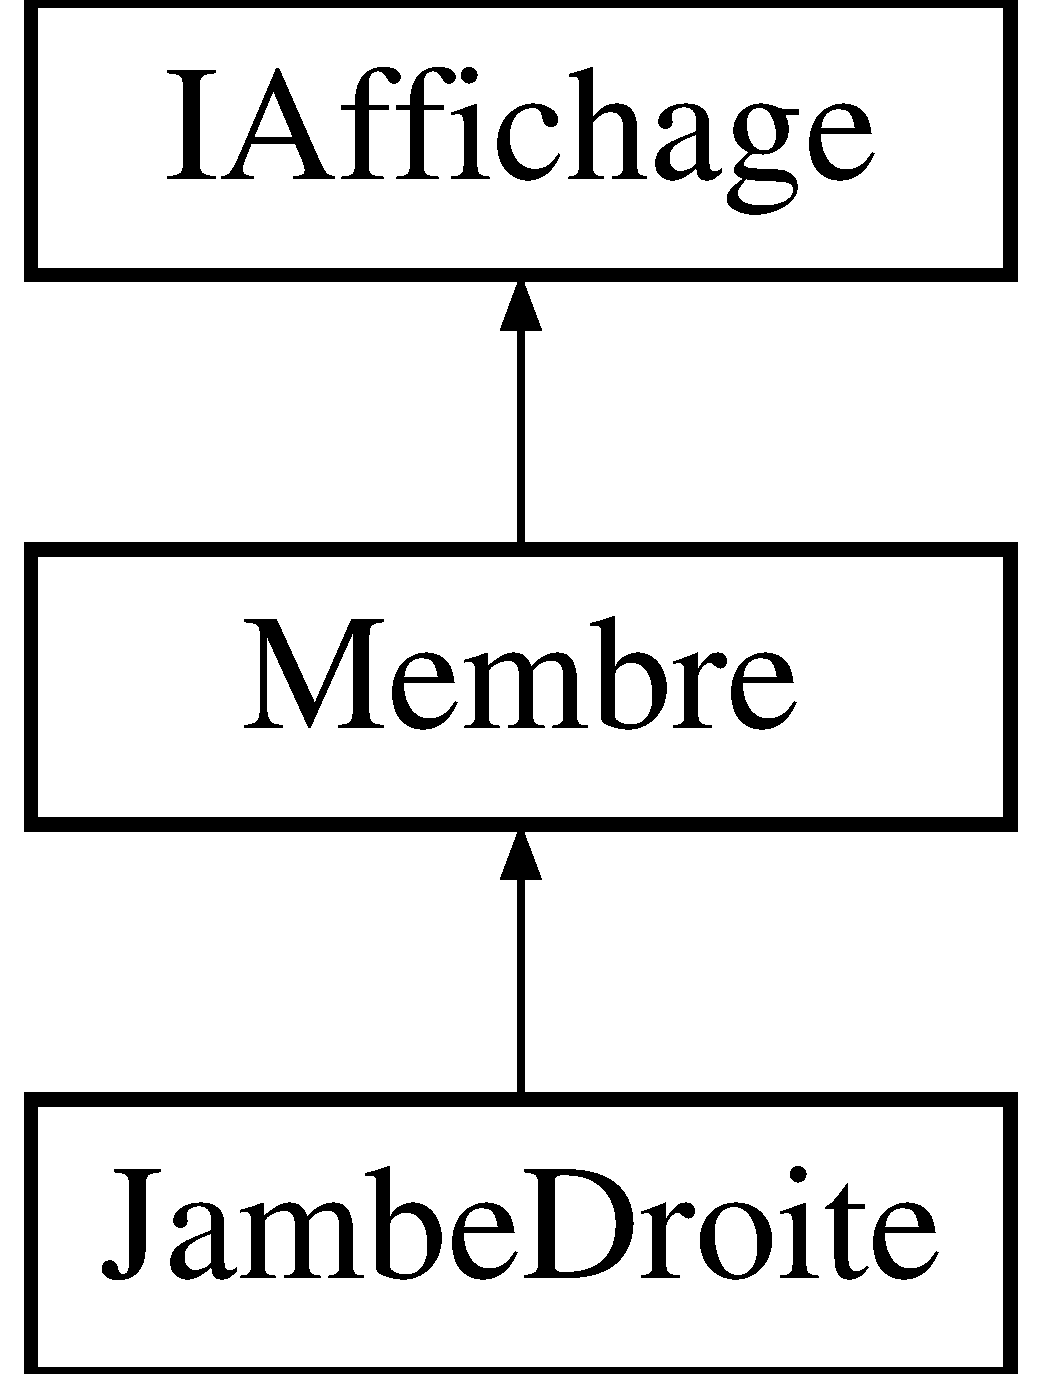
\includegraphics[height=3.000000cm]{class_jambe_droite}
\end{center}
\end{figure}
\subsection*{\-Public \-Member \-Functions}
\begin{DoxyCompactItemize}
\item 
\hyperlink{class_jambe_droite_a22f040786d3645d93c29c131b4041237}{\-Jambe\-Droite} ()
\item 
int \hyperlink{class_jambe_droite_a4dc14c64b239851e5497dc84ca43f6de}{get\-Id} ()
\item 
void \hyperlink{class_jambe_droite_ae8840e4f8b4240a24dbdb7311cf49b45}{set\-Id} (int id)
\item 
int \hyperlink{class_jambe_droite_ab652890a9d08fd39f231dcf9bba48068}{get\-P\-D\-V} ()
\item 
void \hyperlink{class_jambe_droite_a720931176b5219a1ef11e5d255910fbe}{set\-P\-D\-V} (int p)
\item 
int \hyperlink{class_jambe_droite_a236e542d759b7142a42d861612a9ac68}{get\-Libelle} ()
\item 
void \hyperlink{class_jambe_droite_ab45dd17c1fcc3de07b55c13a27bf9699}{set\-Libelle} (string l)
\item 
\hyperlink{class_equipement}{\-Equipement} \hyperlink{class_jambe_droite_a4a9ac6e20a14d99b6db5ce2fd0af4aa0}{get\-Equip} ()
\item 
\hyperlink{class_equipement}{\-Equipement} \hyperlink{class_jambe_droite_a1f8dc857d14b8bfb005dcf633e56f8d3}{set\-Equip} (\hyperlink{class_equipement}{\-Equipement} e)
\end{DoxyCompactItemize}


\subsection{\-Detailed \-Description}
\-Classe \hyperlink{class_jambe_droite}{\-Jambe\-Droite}, hérite de \hyperlink{class_membre}{\-Membre} 

\subsection{\-Constructor \& \-Destructor \-Documentation}
\hypertarget{class_jambe_droite_a22f040786d3645d93c29c131b4041237}{\index{\-Jambe\-Droite@{\-Jambe\-Droite}!\-Jambe\-Droite@{\-Jambe\-Droite}}
\index{\-Jambe\-Droite@{\-Jambe\-Droite}!JambeDroite@{\-Jambe\-Droite}}
\subsubsection[{\-Jambe\-Droite}]{\setlength{\rightskip}{0pt plus 5cm}{\bf \-Jambe\-Droite\-::\-Jambe\-Droite} (
\begin{DoxyParamCaption}
{}
\end{DoxyParamCaption}
)\hspace{0.3cm}{\ttfamily  \mbox{[}inline\mbox{]}}}}\label{class_jambe_droite_a22f040786d3645d93c29c131b4041237}
\-Constructeur explicite initialisant les variables de la jambe droite 

\subsection{\-Member \-Function \-Documentation}
\hypertarget{class_jambe_droite_a4a9ac6e20a14d99b6db5ce2fd0af4aa0}{\index{\-Jambe\-Droite@{\-Jambe\-Droite}!get\-Equip@{get\-Equip}}
\index{get\-Equip@{get\-Equip}!JambeDroite@{\-Jambe\-Droite}}
\subsubsection[{get\-Equip}]{\setlength{\rightskip}{0pt plus 5cm}{\bf \-Equipement} {\bf \-Jambe\-Droite\-::get\-Equip} (
\begin{DoxyParamCaption}
{}
\end{DoxyParamCaption}
)\hspace{0.3cm}{\ttfamily  \mbox{[}inline\mbox{]}}}}\label{class_jambe_droite_a4a9ac6e20a14d99b6db5ce2fd0af4aa0}
\-Accesseur à l'\hyperlink{class_equipement}{\-Equipement} équipé à la jambe droite 

\-Reimplemented from \hyperlink{class_membre_a8b57b95b91806ebf6171624ac0a051cb}{\-Membre}.

\hypertarget{class_jambe_droite_a4dc14c64b239851e5497dc84ca43f6de}{\index{\-Jambe\-Droite@{\-Jambe\-Droite}!get\-Id@{get\-Id}}
\index{get\-Id@{get\-Id}!JambeDroite@{\-Jambe\-Droite}}
\subsubsection[{get\-Id}]{\setlength{\rightskip}{0pt plus 5cm}int {\bf \-Jambe\-Droite\-::get\-Id} (
\begin{DoxyParamCaption}
{}
\end{DoxyParamCaption}
)\hspace{0.3cm}{\ttfamily  \mbox{[}inline\mbox{]}}}}\label{class_jambe_droite_a4dc14c64b239851e5497dc84ca43f6de}
\-Accesseur à l'identifiant de la jambe droite 

\-Reimplemented from \hyperlink{class_membre_aa4ba3c5babf132246cc84907c37e3738}{\-Membre}.

\hypertarget{class_jambe_droite_a236e542d759b7142a42d861612a9ac68}{\index{\-Jambe\-Droite@{\-Jambe\-Droite}!get\-Libelle@{get\-Libelle}}
\index{get\-Libelle@{get\-Libelle}!JambeDroite@{\-Jambe\-Droite}}
\subsubsection[{get\-Libelle}]{\setlength{\rightskip}{0pt plus 5cm}int {\bf \-Jambe\-Droite\-::get\-Libelle} (
\begin{DoxyParamCaption}
{}
\end{DoxyParamCaption}
)\hspace{0.3cm}{\ttfamily  \mbox{[}inline\mbox{]}}}}\label{class_jambe_droite_a236e542d759b7142a42d861612a9ac68}
\-Accesseur au libellé du membre 

\-Reimplemented from \hyperlink{class_membre_a6ef6931754fe7ce7e8101bf27bc3ef6a}{\-Membre}.

\hypertarget{class_jambe_droite_ab652890a9d08fd39f231dcf9bba48068}{\index{\-Jambe\-Droite@{\-Jambe\-Droite}!get\-P\-D\-V@{get\-P\-D\-V}}
\index{get\-P\-D\-V@{get\-P\-D\-V}!JambeDroite@{\-Jambe\-Droite}}
\subsubsection[{get\-P\-D\-V}]{\setlength{\rightskip}{0pt plus 5cm}int {\bf \-Jambe\-Droite\-::get\-P\-D\-V} (
\begin{DoxyParamCaption}
{}
\end{DoxyParamCaption}
)\hspace{0.3cm}{\ttfamily  \mbox{[}inline\mbox{]}}}}\label{class_jambe_droite_ab652890a9d08fd39f231dcf9bba48068}
\-Accesseur au nombre de points de vie de la jambe droite 

\-Reimplemented from \hyperlink{class_membre_a35ddd831b2ca01dd13be213470f2aa65}{\-Membre}.

\hypertarget{class_jambe_droite_a1f8dc857d14b8bfb005dcf633e56f8d3}{\index{\-Jambe\-Droite@{\-Jambe\-Droite}!set\-Equip@{set\-Equip}}
\index{set\-Equip@{set\-Equip}!JambeDroite@{\-Jambe\-Droite}}
\subsubsection[{set\-Equip}]{\setlength{\rightskip}{0pt plus 5cm}{\bf \-Equipement} {\bf \-Jambe\-Droite\-::set\-Equip} (
\begin{DoxyParamCaption}
\item[{{\bf \-Equipement}}]{e}
\end{DoxyParamCaption}
)\hspace{0.3cm}{\ttfamily  \mbox{[}inline\mbox{]}}}}\label{class_jambe_droite_a1f8dc857d14b8bfb005dcf633e56f8d3}
\-Mutateur de l'\hyperlink{class_equipement}{\-Equipement} équipé à la jambe droite 

\-Reimplemented from \hyperlink{class_membre_ab2f78da0480458242168b57cf33e3f7c}{\-Membre}.

\hypertarget{class_jambe_droite_ae8840e4f8b4240a24dbdb7311cf49b45}{\index{\-Jambe\-Droite@{\-Jambe\-Droite}!set\-Id@{set\-Id}}
\index{set\-Id@{set\-Id}!JambeDroite@{\-Jambe\-Droite}}
\subsubsection[{set\-Id}]{\setlength{\rightskip}{0pt plus 5cm}void {\bf \-Jambe\-Droite\-::set\-Id} (
\begin{DoxyParamCaption}
\item[{int}]{id}
\end{DoxyParamCaption}
)\hspace{0.3cm}{\ttfamily  \mbox{[}inline\mbox{]}}}}\label{class_jambe_droite_ae8840e4f8b4240a24dbdb7311cf49b45}
\-Mutateur à l'identifiant de la jambe droite 

\-Reimplemented from \hyperlink{class_membre_a4b87bebc56e82f08d4ebdf8bcf773c11}{\-Membre}.

\hypertarget{class_jambe_droite_ab45dd17c1fcc3de07b55c13a27bf9699}{\index{\-Jambe\-Droite@{\-Jambe\-Droite}!set\-Libelle@{set\-Libelle}}
\index{set\-Libelle@{set\-Libelle}!JambeDroite@{\-Jambe\-Droite}}
\subsubsection[{set\-Libelle}]{\setlength{\rightskip}{0pt plus 5cm}void {\bf \-Jambe\-Droite\-::set\-Libelle} (
\begin{DoxyParamCaption}
\item[{string}]{l}
\end{DoxyParamCaption}
)\hspace{0.3cm}{\ttfamily  \mbox{[}inline\mbox{]}}}}\label{class_jambe_droite_ab45dd17c1fcc3de07b55c13a27bf9699}
\-Mutateur du libellé du membre 

\-Reimplemented from \hyperlink{class_membre_aaffef4990f332871cd1dd9b3fc03a078}{\-Membre}.

\hypertarget{class_jambe_droite_a720931176b5219a1ef11e5d255910fbe}{\index{\-Jambe\-Droite@{\-Jambe\-Droite}!set\-P\-D\-V@{set\-P\-D\-V}}
\index{set\-P\-D\-V@{set\-P\-D\-V}!JambeDroite@{\-Jambe\-Droite}}
\subsubsection[{set\-P\-D\-V}]{\setlength{\rightskip}{0pt plus 5cm}void {\bf \-Jambe\-Droite\-::set\-P\-D\-V} (
\begin{DoxyParamCaption}
\item[{int}]{p}
\end{DoxyParamCaption}
)\hspace{0.3cm}{\ttfamily  \mbox{[}inline\mbox{]}}}}\label{class_jambe_droite_a720931176b5219a1ef11e5d255910fbe}
\-Mutateur du nombre de points de vie de la jambe droite 

\-Reimplemented from \hyperlink{class_membre_a6b45657cd705c02a6ab5a338d1204f3e}{\-Membre}.



\-The documentation for this class was generated from the following file\-:\begin{DoxyCompactItemize}
\item 
\-Projet\-P\-O\-O-\/master/\-Jambe\-Droite.\-cpp\end{DoxyCompactItemize}

\hypertarget{class_jambe_gauche}{\section{\-Jambe\-Gauche \-Class \-Reference}
\label{class_jambe_gauche}\index{\-Jambe\-Gauche@{\-Jambe\-Gauche}}
}
\-Inheritance diagram for \-Jambe\-Gauche\-:\begin{figure}[H]
\begin{center}
\leavevmode
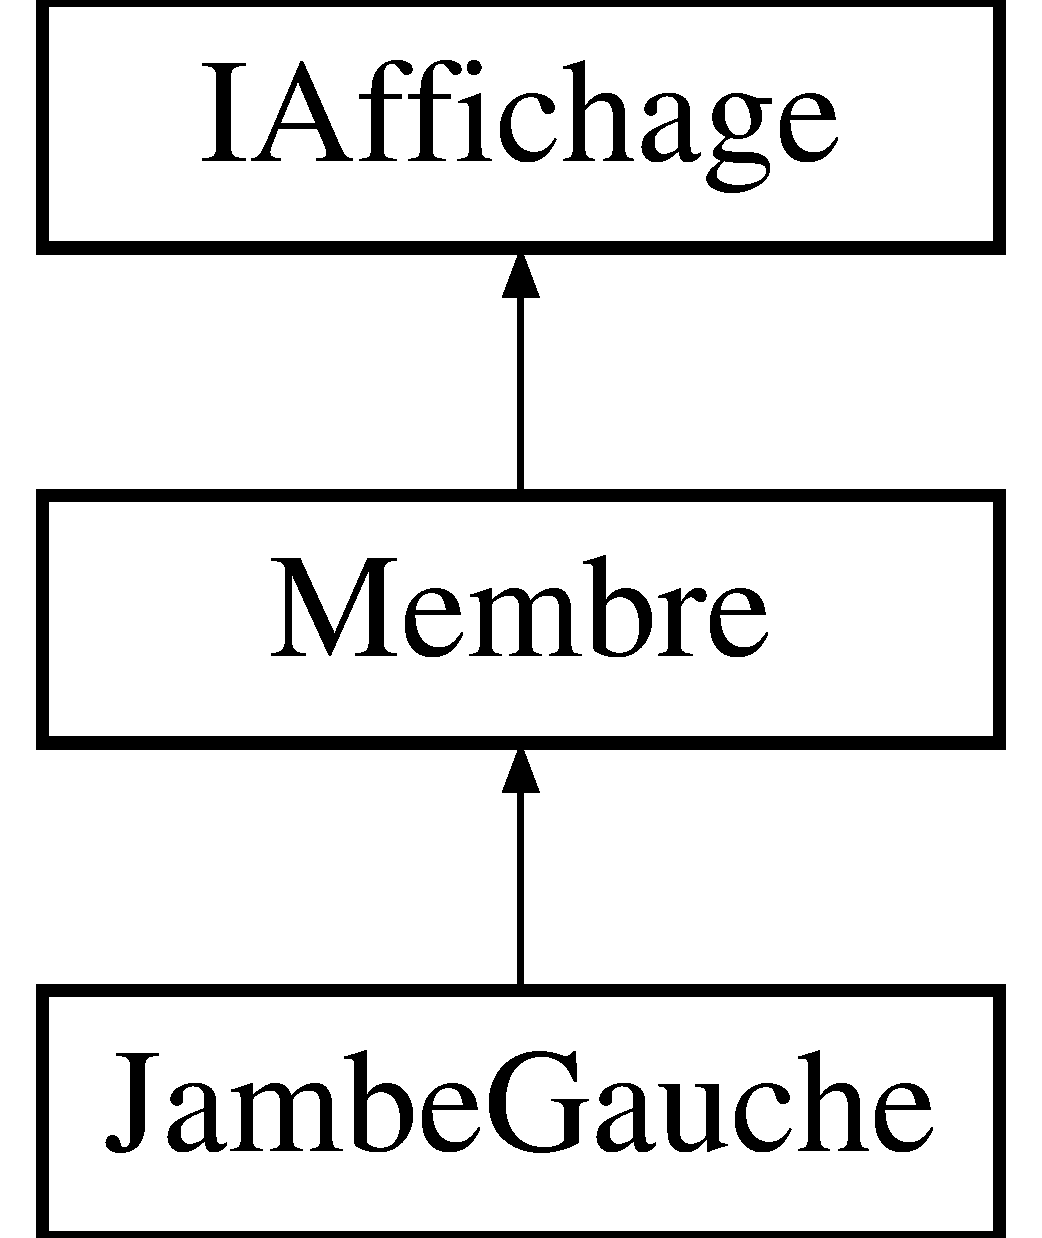
\includegraphics[height=3.000000cm]{class_jambe_gauche}
\end{center}
\end{figure}
\subsection*{\-Public \-Member \-Functions}
\begin{DoxyCompactItemize}
\item 
\hyperlink{class_jambe_gauche_a306ff75914909ceccf6bb47a6f00aa34}{\-Jambe\-Gauche} ()
\item 
int \hyperlink{class_jambe_gauche_a45630c5110de97c6178e23291aa547f0}{get\-Id} ()
\item 
void \hyperlink{class_jambe_gauche_a2851cb622f0d958c2795bcfe45904209}{set\-Id} (int id)
\item 
int \hyperlink{class_jambe_gauche_a0012a7b60f3aa32e26dd59f88f7f046f}{get\-P\-D\-V} ()
\item 
void \hyperlink{class_jambe_gauche_af6fc1b58e9f6dd1eeb840c71d1908043}{set\-P\-D\-V} (int p)
\item 
string \hyperlink{class_jambe_gauche_ab6cacd327fa0c3a9a6084d4d1c52ad51}{get\-Libelle} ()
\item 
void \hyperlink{class_jambe_gauche_a5ce53b166f79dbfb157ccc2774dcdbfd}{set\-Libelle} (string l)
\item 
\hyperlink{class_equipement}{\-Equipement} \hyperlink{class_jambe_gauche_a050999bb1256f3d409c5708be152344a}{get\-Equip} ()
\item 
\hyperlink{class_equipement}{\-Equipement} \hyperlink{class_jambe_gauche_a6192a0c9850adebf39f9ef14344a8957}{set\-Equip} (\hyperlink{class_equipement}{\-Equipement} e)
\end{DoxyCompactItemize}


\subsection{\-Detailed \-Description}
\-Classe \hyperlink{class_jambe_gauche}{\-Jambe\-Gauche}, hérite de \hyperlink{class_membre}{\-Membre} 

\subsection{\-Constructor \& \-Destructor \-Documentation}
\hypertarget{class_jambe_gauche_a306ff75914909ceccf6bb47a6f00aa34}{\index{\-Jambe\-Gauche@{\-Jambe\-Gauche}!\-Jambe\-Gauche@{\-Jambe\-Gauche}}
\index{\-Jambe\-Gauche@{\-Jambe\-Gauche}!JambeGauche@{\-Jambe\-Gauche}}
\subsubsection[{\-Jambe\-Gauche}]{\setlength{\rightskip}{0pt plus 5cm}{\bf \-Jambe\-Gauche\-::\-Jambe\-Gauche} (
\begin{DoxyParamCaption}
{}
\end{DoxyParamCaption}
)\hspace{0.3cm}{\ttfamily  \mbox{[}inline\mbox{]}}}}\label{class_jambe_gauche_a306ff75914909ceccf6bb47a6f00aa34}
\-Constructeur explicite initialisant les variables de la jambe gauche 

\subsection{\-Member \-Function \-Documentation}
\hypertarget{class_jambe_gauche_a050999bb1256f3d409c5708be152344a}{\index{\-Jambe\-Gauche@{\-Jambe\-Gauche}!get\-Equip@{get\-Equip}}
\index{get\-Equip@{get\-Equip}!JambeGauche@{\-Jambe\-Gauche}}
\subsubsection[{get\-Equip}]{\setlength{\rightskip}{0pt plus 5cm}{\bf \-Equipement} {\bf \-Jambe\-Gauche\-::get\-Equip} (
\begin{DoxyParamCaption}
{}
\end{DoxyParamCaption}
)\hspace{0.3cm}{\ttfamily  \mbox{[}inline\mbox{]}}}}\label{class_jambe_gauche_a050999bb1256f3d409c5708be152344a}
\-Accesseur à l'\hyperlink{class_equipement}{\-Equipement} équipé à la jambe gauche 

\-Reimplemented from \hyperlink{class_membre_a8b57b95b91806ebf6171624ac0a051cb}{\-Membre}.

\hypertarget{class_jambe_gauche_a45630c5110de97c6178e23291aa547f0}{\index{\-Jambe\-Gauche@{\-Jambe\-Gauche}!get\-Id@{get\-Id}}
\index{get\-Id@{get\-Id}!JambeGauche@{\-Jambe\-Gauche}}
\subsubsection[{get\-Id}]{\setlength{\rightskip}{0pt plus 5cm}int {\bf \-Jambe\-Gauche\-::get\-Id} (
\begin{DoxyParamCaption}
{}
\end{DoxyParamCaption}
)\hspace{0.3cm}{\ttfamily  \mbox{[}inline\mbox{]}}}}\label{class_jambe_gauche_a45630c5110de97c6178e23291aa547f0}
\-Accesseur à l'identifiant de la jambe gauche 

\-Reimplemented from \hyperlink{class_membre_aa4ba3c5babf132246cc84907c37e3738}{\-Membre}.

\hypertarget{class_jambe_gauche_ab6cacd327fa0c3a9a6084d4d1c52ad51}{\index{\-Jambe\-Gauche@{\-Jambe\-Gauche}!get\-Libelle@{get\-Libelle}}
\index{get\-Libelle@{get\-Libelle}!JambeGauche@{\-Jambe\-Gauche}}
\subsubsection[{get\-Libelle}]{\setlength{\rightskip}{0pt plus 5cm}string {\bf \-Jambe\-Gauche\-::get\-Libelle} (
\begin{DoxyParamCaption}
{}
\end{DoxyParamCaption}
)\hspace{0.3cm}{\ttfamily  \mbox{[}inline\mbox{]}}}}\label{class_jambe_gauche_ab6cacd327fa0c3a9a6084d4d1c52ad51}
\-Accesseur au libellé du membre 

\-Reimplemented from \hyperlink{class_membre_a6ef6931754fe7ce7e8101bf27bc3ef6a}{\-Membre}.

\hypertarget{class_jambe_gauche_a0012a7b60f3aa32e26dd59f88f7f046f}{\index{\-Jambe\-Gauche@{\-Jambe\-Gauche}!get\-P\-D\-V@{get\-P\-D\-V}}
\index{get\-P\-D\-V@{get\-P\-D\-V}!JambeGauche@{\-Jambe\-Gauche}}
\subsubsection[{get\-P\-D\-V}]{\setlength{\rightskip}{0pt plus 5cm}int {\bf \-Jambe\-Gauche\-::get\-P\-D\-V} (
\begin{DoxyParamCaption}
{}
\end{DoxyParamCaption}
)\hspace{0.3cm}{\ttfamily  \mbox{[}inline\mbox{]}}}}\label{class_jambe_gauche_a0012a7b60f3aa32e26dd59f88f7f046f}
\-Accesseur au nombre de points de vie de la jambe gauche 

\-Reimplemented from \hyperlink{class_membre_a35ddd831b2ca01dd13be213470f2aa65}{\-Membre}.

\hypertarget{class_jambe_gauche_a6192a0c9850adebf39f9ef14344a8957}{\index{\-Jambe\-Gauche@{\-Jambe\-Gauche}!set\-Equip@{set\-Equip}}
\index{set\-Equip@{set\-Equip}!JambeGauche@{\-Jambe\-Gauche}}
\subsubsection[{set\-Equip}]{\setlength{\rightskip}{0pt plus 5cm}{\bf \-Equipement} {\bf \-Jambe\-Gauche\-::set\-Equip} (
\begin{DoxyParamCaption}
\item[{{\bf \-Equipement}}]{e}
\end{DoxyParamCaption}
)\hspace{0.3cm}{\ttfamily  \mbox{[}inline\mbox{]}}}}\label{class_jambe_gauche_a6192a0c9850adebf39f9ef14344a8957}
\-Mutateur de l'\hyperlink{class_equipement}{\-Equipement} équipé à la jambe gauche 

\-Reimplemented from \hyperlink{class_membre_ab2f78da0480458242168b57cf33e3f7c}{\-Membre}.

\hypertarget{class_jambe_gauche_a2851cb622f0d958c2795bcfe45904209}{\index{\-Jambe\-Gauche@{\-Jambe\-Gauche}!set\-Id@{set\-Id}}
\index{set\-Id@{set\-Id}!JambeGauche@{\-Jambe\-Gauche}}
\subsubsection[{set\-Id}]{\setlength{\rightskip}{0pt plus 5cm}void {\bf \-Jambe\-Gauche\-::set\-Id} (
\begin{DoxyParamCaption}
\item[{int}]{id}
\end{DoxyParamCaption}
)\hspace{0.3cm}{\ttfamily  \mbox{[}inline\mbox{]}}}}\label{class_jambe_gauche_a2851cb622f0d958c2795bcfe45904209}
\-Mutateur de l'identifiant de la jambe gauche 

\-Reimplemented from \hyperlink{class_membre_a4b87bebc56e82f08d4ebdf8bcf773c11}{\-Membre}.

\hypertarget{class_jambe_gauche_a5ce53b166f79dbfb157ccc2774dcdbfd}{\index{\-Jambe\-Gauche@{\-Jambe\-Gauche}!set\-Libelle@{set\-Libelle}}
\index{set\-Libelle@{set\-Libelle}!JambeGauche@{\-Jambe\-Gauche}}
\subsubsection[{set\-Libelle}]{\setlength{\rightskip}{0pt plus 5cm}void {\bf \-Jambe\-Gauche\-::set\-Libelle} (
\begin{DoxyParamCaption}
\item[{string}]{l}
\end{DoxyParamCaption}
)\hspace{0.3cm}{\ttfamily  \mbox{[}inline\mbox{]}}}}\label{class_jambe_gauche_a5ce53b166f79dbfb157ccc2774dcdbfd}
\-Mutateur du libellé du membre 

\-Reimplemented from \hyperlink{class_membre_aaffef4990f332871cd1dd9b3fc03a078}{\-Membre}.

\hypertarget{class_jambe_gauche_af6fc1b58e9f6dd1eeb840c71d1908043}{\index{\-Jambe\-Gauche@{\-Jambe\-Gauche}!set\-P\-D\-V@{set\-P\-D\-V}}
\index{set\-P\-D\-V@{set\-P\-D\-V}!JambeGauche@{\-Jambe\-Gauche}}
\subsubsection[{set\-P\-D\-V}]{\setlength{\rightskip}{0pt plus 5cm}void {\bf \-Jambe\-Gauche\-::set\-P\-D\-V} (
\begin{DoxyParamCaption}
\item[{int}]{p}
\end{DoxyParamCaption}
)\hspace{0.3cm}{\ttfamily  \mbox{[}inline\mbox{]}}}}\label{class_jambe_gauche_af6fc1b58e9f6dd1eeb840c71d1908043}
\-Mutateur du nombre de points de vie de la jambe gauche 

\-Reimplemented from \hyperlink{class_membre_a6b45657cd705c02a6ab5a338d1204f3e}{\-Membre}.



\-The documentation for this class was generated from the following file\-:\begin{DoxyCompactItemize}
\item 
\-Projet\-P\-O\-O-\/master/\-Jambe\-Gauche.\-cpp\end{DoxyCompactItemize}

\hypertarget{class_jambiere}{\section{\-Jambiere \-Class \-Reference}
\label{class_jambiere}\index{\-Jambiere@{\-Jambiere}}
}
\-Inheritance diagram for \-Jambiere\-:\begin{figure}[H]
\begin{center}
\leavevmode
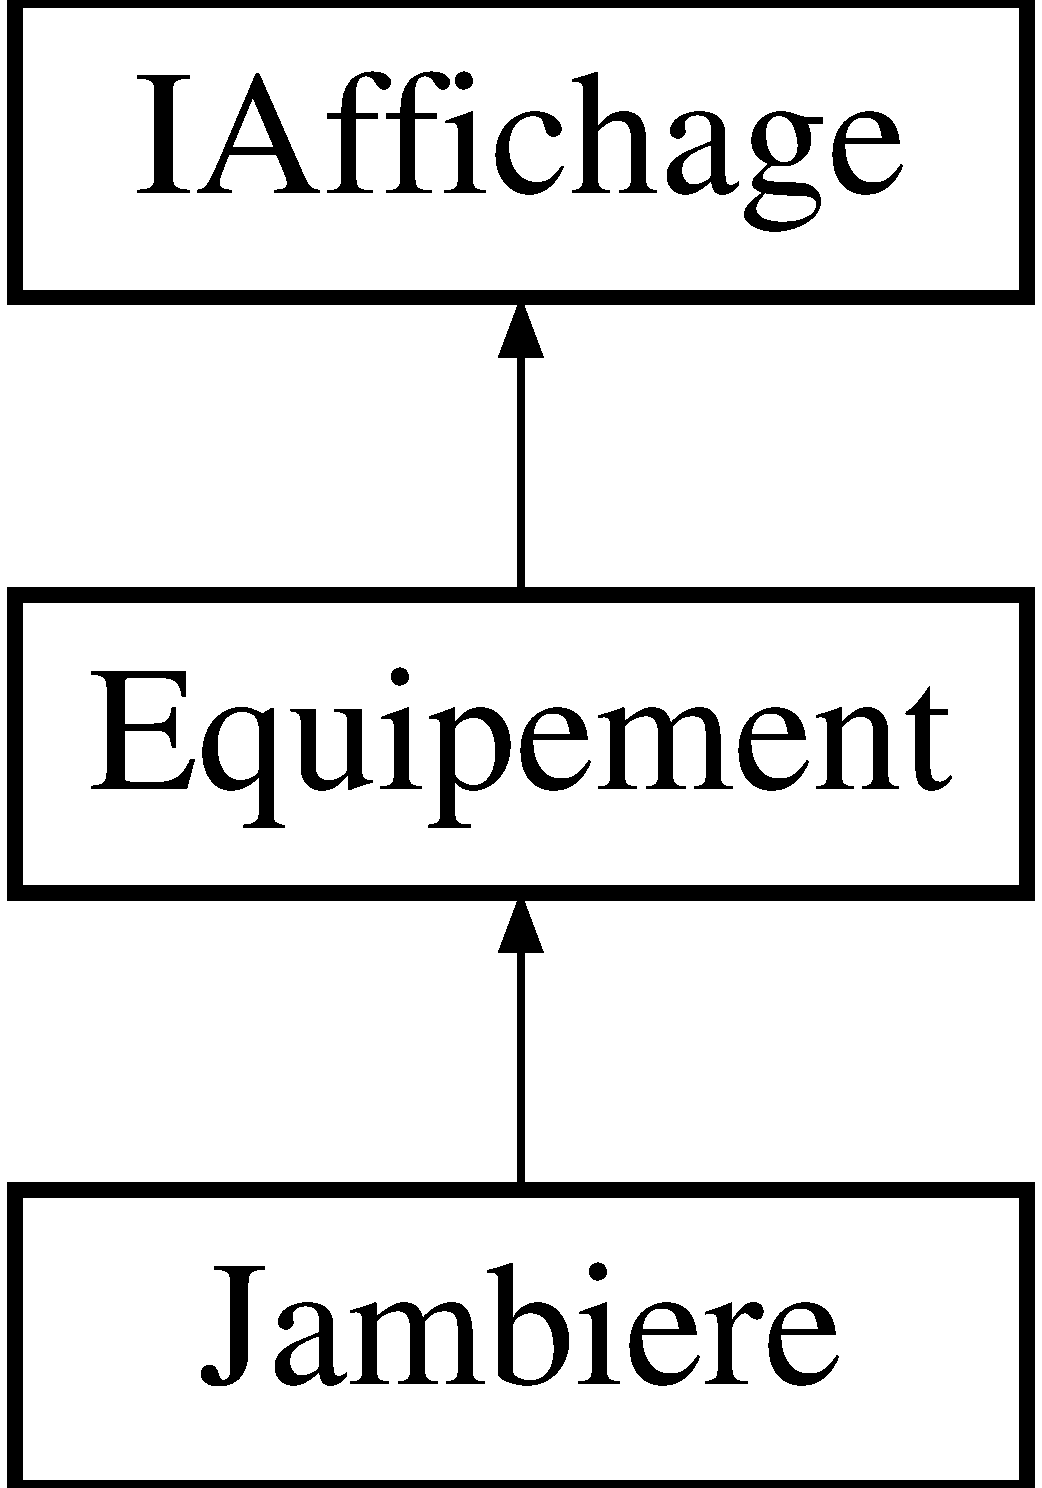
\includegraphics[height=3.000000cm]{class_jambiere}
\end{center}
\end{figure}
\subsection*{\-Public \-Member \-Functions}
\begin{DoxyCompactItemize}
\item 
\hyperlink{class_jambiere_a392269ea14d42c8cd78352e963fdc401}{\-Jambiere} ()
\item 
int \hyperlink{class_jambiere_af22ba3e8b9617ff4e5930509b9adb9f4}{get\-Id} ()
\item 
void \hyperlink{class_jambiere_ae0342539454ecb5c5170bb8d27a3130e}{set\-Id} (int id)
\item 
string \hyperlink{class_jambiere_ad798b9a2d5e43a09aedc606eec7df9a2}{get\-Libelle} ()
\item 
void \hyperlink{class_jambiere_a1a60e57d9792353e77a88884e173ed71}{set\-Libelle} (string l)
\item 
int \hyperlink{class_jambiere_a05c9fa271a51edccbd559a29ca45fe60}{get\-Val\-Def} ()
\item 
void \hyperlink{class_jambiere_ac13c334f7999987cd1437687bb5ad4d4}{set\-Val\-Def} (int v)
\end{DoxyCompactItemize}


\subsection{\-Detailed \-Description}
\-Classe \hyperlink{class_jambiere}{\-Jambiere}, hérite d'\hyperlink{class_equipement}{\-Equipement} 

\subsection{\-Constructor \& \-Destructor \-Documentation}
\hypertarget{class_jambiere_a392269ea14d42c8cd78352e963fdc401}{\index{\-Jambiere@{\-Jambiere}!\-Jambiere@{\-Jambiere}}
\index{\-Jambiere@{\-Jambiere}!Jambiere@{\-Jambiere}}
\subsubsection[{\-Jambiere}]{\setlength{\rightskip}{0pt plus 5cm}{\bf \-Jambiere\-::\-Jambiere} (
\begin{DoxyParamCaption}
{}
\end{DoxyParamCaption}
)\hspace{0.3cm}{\ttfamily  \mbox{[}inline\mbox{]}}}}\label{class_jambiere_a392269ea14d42c8cd78352e963fdc401}
\-Constructeur explicite initialisant les variables de la jambière 

\subsection{\-Member \-Function \-Documentation}
\hypertarget{class_jambiere_af22ba3e8b9617ff4e5930509b9adb9f4}{\index{\-Jambiere@{\-Jambiere}!get\-Id@{get\-Id}}
\index{get\-Id@{get\-Id}!Jambiere@{\-Jambiere}}
\subsubsection[{get\-Id}]{\setlength{\rightskip}{0pt plus 5cm}int {\bf \-Jambiere\-::get\-Id} (
\begin{DoxyParamCaption}
{}
\end{DoxyParamCaption}
)\hspace{0.3cm}{\ttfamily  \mbox{[}inline\mbox{]}}}}\label{class_jambiere_af22ba3e8b9617ff4e5930509b9adb9f4}
\-Accesseur à l'identifiant de la jambière 

\-Reimplemented from \hyperlink{class_equipement_abc38941f5a9deed943b7a83ce69539c3}{\-Equipement}.

\hypertarget{class_jambiere_ad798b9a2d5e43a09aedc606eec7df9a2}{\index{\-Jambiere@{\-Jambiere}!get\-Libelle@{get\-Libelle}}
\index{get\-Libelle@{get\-Libelle}!Jambiere@{\-Jambiere}}
\subsubsection[{get\-Libelle}]{\setlength{\rightskip}{0pt plus 5cm}string {\bf \-Jambiere\-::get\-Libelle} (
\begin{DoxyParamCaption}
{}
\end{DoxyParamCaption}
)\hspace{0.3cm}{\ttfamily  \mbox{[}inline\mbox{]}}}}\label{class_jambiere_ad798b9a2d5e43a09aedc606eec7df9a2}
\-Accesseur au libellé de l'équipement 

\-Reimplemented from \hyperlink{class_equipement_ab00ec565966647bf6edeb1a9df430aa6}{\-Equipement}.

\hypertarget{class_jambiere_a05c9fa271a51edccbd559a29ca45fe60}{\index{\-Jambiere@{\-Jambiere}!get\-Val\-Def@{get\-Val\-Def}}
\index{get\-Val\-Def@{get\-Val\-Def}!Jambiere@{\-Jambiere}}
\subsubsection[{get\-Val\-Def}]{\setlength{\rightskip}{0pt plus 5cm}int {\bf \-Jambiere\-::get\-Val\-Def} (
\begin{DoxyParamCaption}
{}
\end{DoxyParamCaption}
)\hspace{0.3cm}{\ttfamily  \mbox{[}inline\mbox{]}}}}\label{class_jambiere_a05c9fa271a51edccbd559a29ca45fe60}
\-Accesseur à la valeur de défense de la jambière 

\-Reimplemented from \hyperlink{class_equipement_a7b3003f4da24a94bfec94555e35e772c}{\-Equipement}.

\hypertarget{class_jambiere_ae0342539454ecb5c5170bb8d27a3130e}{\index{\-Jambiere@{\-Jambiere}!set\-Id@{set\-Id}}
\index{set\-Id@{set\-Id}!Jambiere@{\-Jambiere}}
\subsubsection[{set\-Id}]{\setlength{\rightskip}{0pt plus 5cm}void {\bf \-Jambiere\-::set\-Id} (
\begin{DoxyParamCaption}
\item[{int}]{id}
\end{DoxyParamCaption}
)\hspace{0.3cm}{\ttfamily  \mbox{[}inline\mbox{]}}}}\label{class_jambiere_ae0342539454ecb5c5170bb8d27a3130e}
\-Mutateur de l'identifiant de la jambière 

\-Reimplemented from \hyperlink{class_equipement_a98208826ad05cbc38211e9f70bd908c5}{\-Equipement}.

\hypertarget{class_jambiere_a1a60e57d9792353e77a88884e173ed71}{\index{\-Jambiere@{\-Jambiere}!set\-Libelle@{set\-Libelle}}
\index{set\-Libelle@{set\-Libelle}!Jambiere@{\-Jambiere}}
\subsubsection[{set\-Libelle}]{\setlength{\rightskip}{0pt plus 5cm}void {\bf \-Jambiere\-::set\-Libelle} (
\begin{DoxyParamCaption}
\item[{string}]{l}
\end{DoxyParamCaption}
)\hspace{0.3cm}{\ttfamily  \mbox{[}inline\mbox{]}}}}\label{class_jambiere_a1a60e57d9792353e77a88884e173ed71}
\-Mutateur du libellé de l'équipement 

\-Reimplemented from \hyperlink{class_equipement_aea246b68c747bd5ec84ca8ce4c4c7b40}{\-Equipement}.

\hypertarget{class_jambiere_ac13c334f7999987cd1437687bb5ad4d4}{\index{\-Jambiere@{\-Jambiere}!set\-Val\-Def@{set\-Val\-Def}}
\index{set\-Val\-Def@{set\-Val\-Def}!Jambiere@{\-Jambiere}}
\subsubsection[{set\-Val\-Def}]{\setlength{\rightskip}{0pt plus 5cm}void {\bf \-Jambiere\-::set\-Val\-Def} (
\begin{DoxyParamCaption}
\item[{int}]{v}
\end{DoxyParamCaption}
)\hspace{0.3cm}{\ttfamily  \mbox{[}inline\mbox{]}}}}\label{class_jambiere_ac13c334f7999987cd1437687bb5ad4d4}
\-Mutateur de la valeur de défense de la jambière 

\-Reimplemented from \hyperlink{class_equipement_ad9940c901b3a96b91c5c3f24713face5}{\-Equipement}.



\-The documentation for this class was generated from the following file\-:\begin{DoxyCompactItemize}
\item 
\-Projet\-P\-O\-O-\/master/\-Jambiere.\-cpp\end{DoxyCompactItemize}

\hypertarget{class_javelot}{\section{\-Javelot \-Class \-Reference}
\label{class_javelot}\index{\-Javelot@{\-Javelot}}
}
\-Inheritance diagram for \-Javelot\-:\begin{figure}[H]
\begin{center}
\leavevmode
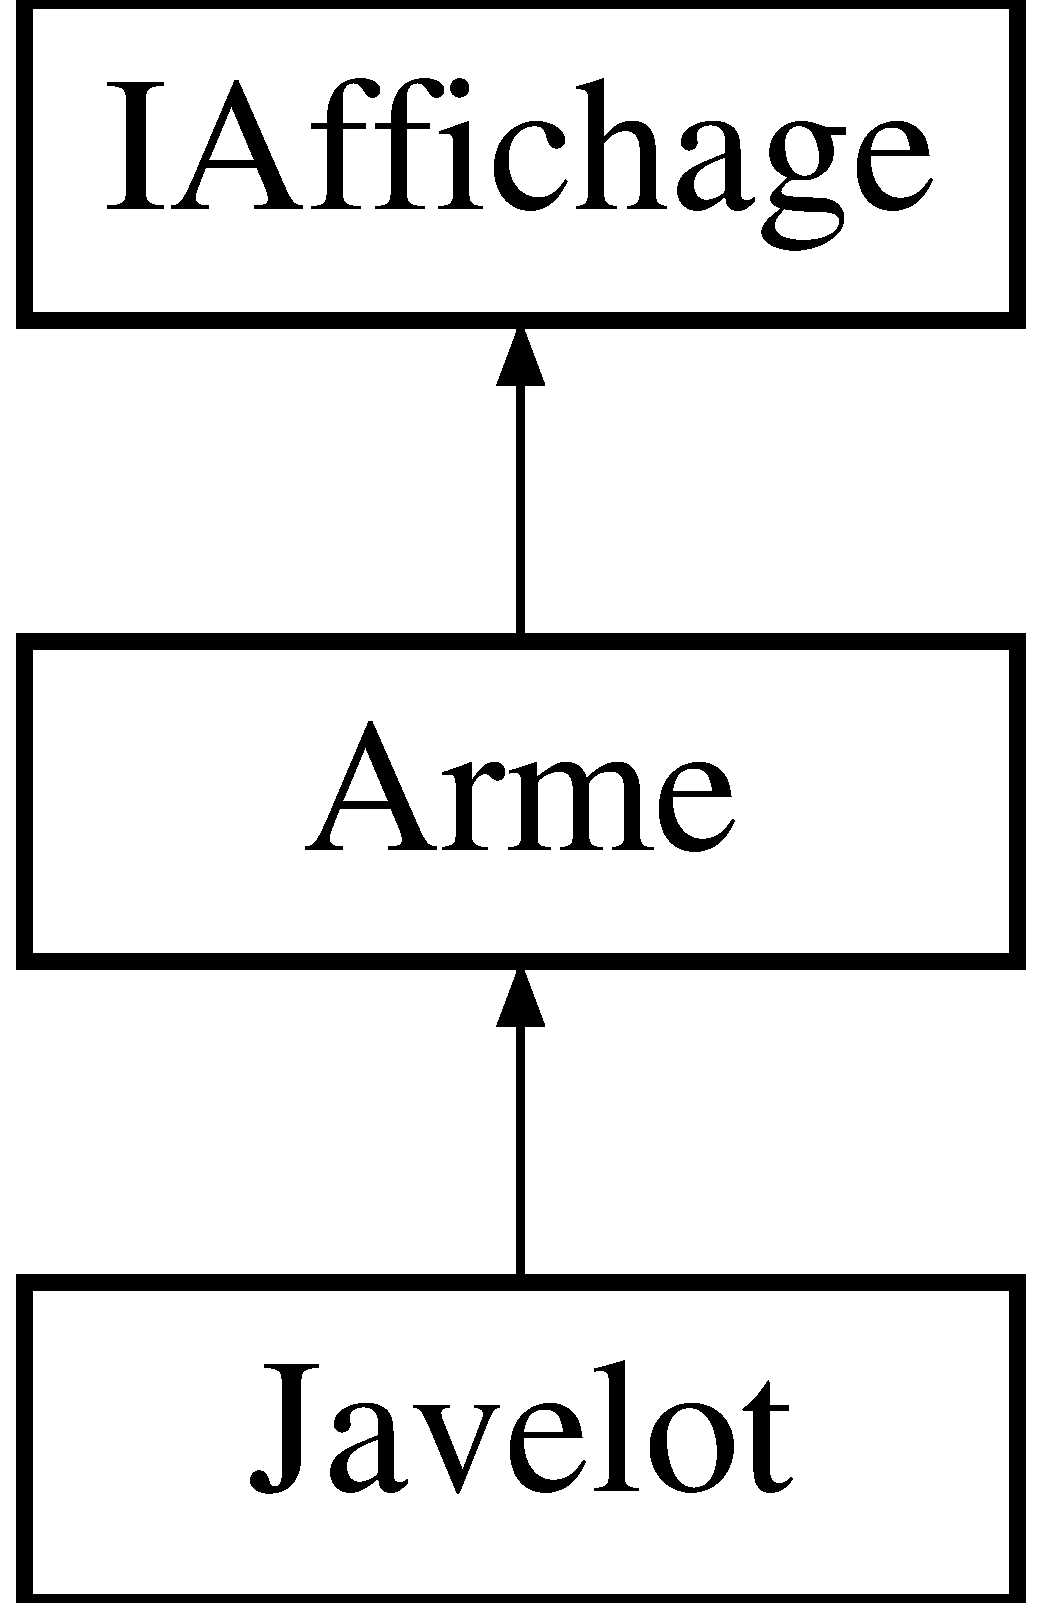
\includegraphics[height=3.000000cm]{class_javelot}
\end{center}
\end{figure}
\subsection*{\-Public \-Member \-Functions}
\begin{DoxyCompactItemize}
\item 
\hyperlink{class_javelot_ab98542adcc1824a91579544f4d9c0004}{\-Javelot} ()
\item 
int \hyperlink{class_javelot_aba1cccb47bf10d583936eae96284f49b}{get\-Id} ()
\item 
void \hyperlink{class_javelot_ab84399b82fc67e7ecf3c08081f24fec4}{set\-Id} (int id)
\item 
string \hyperlink{class_javelot_a37dca37b0f1756ad08352fe200fb6ed7}{get\-Libelle} ()
\item 
void \hyperlink{class_javelot_a66872fd5e6d4a5704ec3c67264938f8e}{set\-Libelle} (string l)
\item 
int \hyperlink{class_javelot_a3072bb4abd2e30937241bd63538a5f4f}{get\-Val\-Deg} ()
\item 
void \hyperlink{class_javelot_ab732b9939709e6cd0a1d9e47849ac80b}{set\-Val\-Deg} (int v)
\end{DoxyCompactItemize}


\subsection{\-Detailed \-Description}
\-Classe \hyperlink{class_javelot}{\-Javelot}, hérite d'\hyperlink{class_arme}{\-Arme} 

\subsection{\-Constructor \& \-Destructor \-Documentation}
\hypertarget{class_javelot_ab98542adcc1824a91579544f4d9c0004}{\index{\-Javelot@{\-Javelot}!\-Javelot@{\-Javelot}}
\index{\-Javelot@{\-Javelot}!Javelot@{\-Javelot}}
\subsubsection[{\-Javelot}]{\setlength{\rightskip}{0pt plus 5cm}{\bf \-Javelot\-::\-Javelot} (
\begin{DoxyParamCaption}
{}
\end{DoxyParamCaption}
)\hspace{0.3cm}{\ttfamily  \mbox{[}inline\mbox{]}}}}\label{class_javelot_ab98542adcc1824a91579544f4d9c0004}
\-Constructeur explicite initialisant les variables du javelot 

\subsection{\-Member \-Function \-Documentation}
\hypertarget{class_javelot_aba1cccb47bf10d583936eae96284f49b}{\index{\-Javelot@{\-Javelot}!get\-Id@{get\-Id}}
\index{get\-Id@{get\-Id}!Javelot@{\-Javelot}}
\subsubsection[{get\-Id}]{\setlength{\rightskip}{0pt plus 5cm}int {\bf \-Javelot\-::get\-Id} (
\begin{DoxyParamCaption}
{}
\end{DoxyParamCaption}
)\hspace{0.3cm}{\ttfamily  \mbox{[}inline\mbox{]}}}}\label{class_javelot_aba1cccb47bf10d583936eae96284f49b}
\-Accesseur à l'identifiant du javelot 

\-Reimplemented from \hyperlink{class_arme_a6c957484697d9ad38ab1ed4361f3b8f4}{\-Arme}.

\hypertarget{class_javelot_a37dca37b0f1756ad08352fe200fb6ed7}{\index{\-Javelot@{\-Javelot}!get\-Libelle@{get\-Libelle}}
\index{get\-Libelle@{get\-Libelle}!Javelot@{\-Javelot}}
\subsubsection[{get\-Libelle}]{\setlength{\rightskip}{0pt plus 5cm}string {\bf \-Javelot\-::get\-Libelle} (
\begin{DoxyParamCaption}
{}
\end{DoxyParamCaption}
)\hspace{0.3cm}{\ttfamily  \mbox{[}inline\mbox{]}}}}\label{class_javelot_a37dca37b0f1756ad08352fe200fb6ed7}
\-Accesseur au libellé de l'arme 

\-Reimplemented from \hyperlink{class_arme_a5e43d33d0e14da19fb37dc497474135b}{\-Arme}.

\hypertarget{class_javelot_a3072bb4abd2e30937241bd63538a5f4f}{\index{\-Javelot@{\-Javelot}!get\-Val\-Deg@{get\-Val\-Deg}}
\index{get\-Val\-Deg@{get\-Val\-Deg}!Javelot@{\-Javelot}}
\subsubsection[{get\-Val\-Deg}]{\setlength{\rightskip}{0pt plus 5cm}int {\bf \-Javelot\-::get\-Val\-Deg} (
\begin{DoxyParamCaption}
{}
\end{DoxyParamCaption}
)\hspace{0.3cm}{\ttfamily  \mbox{[}inline\mbox{]}}}}\label{class_javelot_a3072bb4abd2e30937241bd63538a5f4f}
\-Accesseur à la valeur de dégâts du javelot \hypertarget{class_javelot_ab84399b82fc67e7ecf3c08081f24fec4}{\index{\-Javelot@{\-Javelot}!set\-Id@{set\-Id}}
\index{set\-Id@{set\-Id}!Javelot@{\-Javelot}}
\subsubsection[{set\-Id}]{\setlength{\rightskip}{0pt plus 5cm}void {\bf \-Javelot\-::set\-Id} (
\begin{DoxyParamCaption}
\item[{int}]{id}
\end{DoxyParamCaption}
)\hspace{0.3cm}{\ttfamily  \mbox{[}inline\mbox{]}}}}\label{class_javelot_ab84399b82fc67e7ecf3c08081f24fec4}
\-Mutateur de l'identifiant du javelot 

\-Reimplemented from \hyperlink{class_arme_a332699f4c7b2dab9e38fccfddba7275b}{\-Arme}.

\hypertarget{class_javelot_a66872fd5e6d4a5704ec3c67264938f8e}{\index{\-Javelot@{\-Javelot}!set\-Libelle@{set\-Libelle}}
\index{set\-Libelle@{set\-Libelle}!Javelot@{\-Javelot}}
\subsubsection[{set\-Libelle}]{\setlength{\rightskip}{0pt plus 5cm}void {\bf \-Javelot\-::set\-Libelle} (
\begin{DoxyParamCaption}
\item[{string}]{l}
\end{DoxyParamCaption}
)\hspace{0.3cm}{\ttfamily  \mbox{[}inline\mbox{]}}}}\label{class_javelot_a66872fd5e6d4a5704ec3c67264938f8e}
\-Mutateur du libellé de l'arme 

\-Reimplemented from \hyperlink{class_arme_ab38eebb032ab6773678ee40f152df6dd}{\-Arme}.

\hypertarget{class_javelot_ab732b9939709e6cd0a1d9e47849ac80b}{\index{\-Javelot@{\-Javelot}!set\-Val\-Deg@{set\-Val\-Deg}}
\index{set\-Val\-Deg@{set\-Val\-Deg}!Javelot@{\-Javelot}}
\subsubsection[{set\-Val\-Deg}]{\setlength{\rightskip}{0pt plus 5cm}void {\bf \-Javelot\-::set\-Val\-Deg} (
\begin{DoxyParamCaption}
\item[{int}]{v}
\end{DoxyParamCaption}
)\hspace{0.3cm}{\ttfamily  \mbox{[}inline\mbox{]}}}}\label{class_javelot_ab732b9939709e6cd0a1d9e47849ac80b}
\-Mutateur de la valeur de dégâts du javelot 

\-The documentation for this class was generated from the following file\-:\begin{DoxyCompactItemize}
\item 
\-Projet\-P\-O\-O-\/master/\-Javelot.\-cpp\end{DoxyCompactItemize}

\hypertarget{class_jeu}{\section{\-Jeu \-Class \-Reference}
\label{class_jeu}\index{\-Jeu@{\-Jeu}}
}
\-Inheritance diagram for \-Jeu\-:\begin{figure}[H]
\begin{center}
\leavevmode
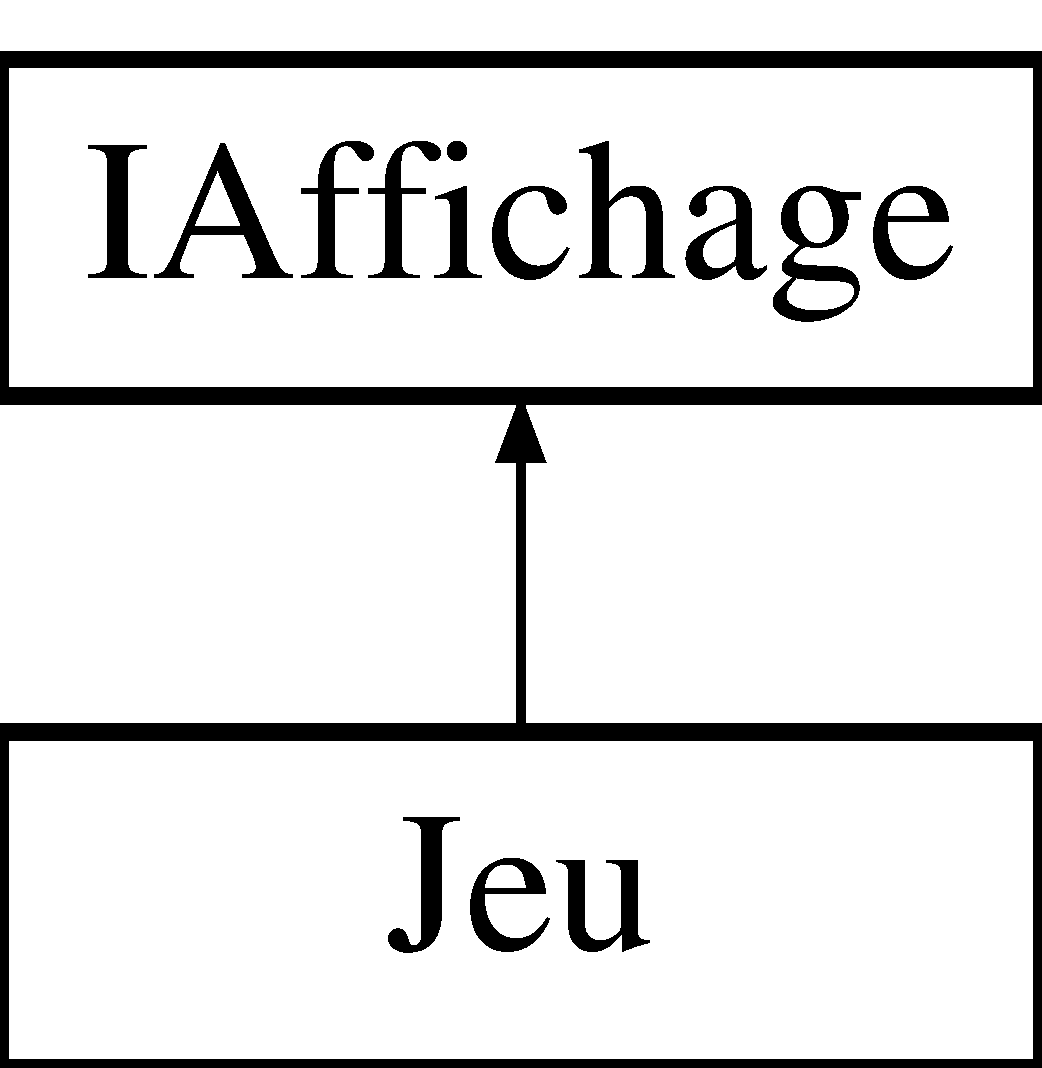
\includegraphics[height=2.000000cm]{class_jeu}
\end{center}
\end{figure}
\subsection*{\-Public \-Types}
\begin{DoxyCompactItemize}
\item 
enum {\bfseries types} \{ \*
{\bfseries \-D\-I\-M\-A\-C\-H\-A\-E\-R\-U\-S} =  1, 
{\bfseries \-R\-E\-T\-I\-A\-R\-I\-U\-S} =  2, 
{\bfseries \-M\-U\-R\-M\-I\-L\-L\-O} =  3, 
{\bfseries \-V\-E\-L\-I\-T\-E} =  4, 
\*
{\bfseries \-T\-H\-R\-A\-E\-X} =  5, 
{\bfseries \-S\-E\-C\-U\-T\-O\-R} =  6
 \}
\end{DoxyCompactItemize}
\subsection*{\-Public \-Member \-Functions}
\begin{DoxyCompactItemize}
\item 
\hypertarget{class_jeu_afc8d47d5af8133e555e0e02641dc03c9}{void {\bfseries recup\-Last\-Id} ()}\label{class_jeu_afc8d47d5af8133e555e0e02641dc03c9}

\item 
\hypertarget{class_jeu_ac2dc12316aef3df5ffc04ace0d2ca8a3}{void {\bfseries maj\-Last\-Id} (int i)}\label{class_jeu_ac2dc12316aef3df5ffc04ace0d2ca8a3}

\item 
\hypertarget{class_jeu_ac24053e79c6d689613eb43f33a849669}{void {\bfseries recup\-Perso} ()}\label{class_jeu_ac24053e79c6d689613eb43f33a849669}

\item 
\hypertarget{class_jeu_ae02adb2fa1ed4e84bc008fdea4c187a7}{void {\bfseries afficher\-Menu\-Principal} ()}\label{class_jeu_ae02adb2fa1ed4e84bc008fdea4c187a7}

\item 
\hypertarget{class_jeu_add76b474564ae0205343d3b995b43075}{void {\bfseries creer\-Personnage} ()}\label{class_jeu_add76b474564ae0205343d3b995b43075}

\item 
\hypertarget{class_jeu_a322a4c1a4084a44b0c5fb1cff5037391}{void {\bfseries enregistrer\-Nouveau\-Perso} (int id, string nom, int type)}\label{class_jeu_a322a4c1a4084a44b0c5fb1cff5037391}

\item 
\hypertarget{class_jeu_a7dd7448e4889305f0ea21679b16d2df1}{void {\bfseries chargement\-Persos} ()}\label{class_jeu_a7dd7448e4889305f0ea21679b16d2df1}

\item 
void \hyperlink{class_jeu_a40747c204660ad830d76378d0cbac1f0}{afficher\-Info} ()
\item 
\hypertarget{class_jeu_a0258b4e17a825904fa41213351bcd811}{void {\bfseries commencer\-Partie} ()}\label{class_jeu_a0258b4e17a825904fa41213351bcd811}

\item 
\hypertarget{class_jeu_a3fe3cdfb2476146d904fd9800eb932f4}{bool {\bfseries is\-Joueur\-Courant} (int id\-Perso)}\label{class_jeu_a3fe3cdfb2476146d904fd9800eb932f4}

\item 
\hypertarget{class_jeu_acc947eec44204b9f472a8b4b7fb41a25}{int {\bfseries get\-Joueur\-Courant} ()}\label{class_jeu_acc947eec44204b9f472a8b4b7fb41a25}

\item 
\hypertarget{class_jeu_a88d92d04311a3bea94fe4c5972a4dec7}{void {\bfseries set\-Joueur\-Courant} (int i)}\label{class_jeu_a88d92d04311a3bea94fe4c5972a4dec7}

\item 
\hypertarget{class_jeu_a7869b56cb07ad313c2227a7d8c470701}{void {\bfseries porter\-Coup} (int id\-Perso, int id\-Membre)}\label{class_jeu_a7869b56cb07ad313c2227a7d8c470701}

\end{DoxyCompactItemize}


\subsection{\-Detailed \-Description}
\-Classe \hyperlink{class_jeu}{\-Jeu} \-Implémente l'interface \hyperlink{class_i_affichage}{\-I\-Affichage} 

\subsection{\-Member \-Function \-Documentation}
\hypertarget{class_jeu_a40747c204660ad830d76378d0cbac1f0}{\index{\-Jeu@{\-Jeu}!afficher\-Info@{afficher\-Info}}
\index{afficher\-Info@{afficher\-Info}!Jeu@{\-Jeu}}
\subsubsection[{afficher\-Info}]{\setlength{\rightskip}{0pt plus 5cm}void {\bf \-Jeu\-::afficher\-Info} (
\begin{DoxyParamCaption}
{}
\end{DoxyParamCaption}
)\hspace{0.3cm}{\ttfamily  \mbox{[}inline, virtual\mbox{]}}}}\label{class_jeu_a40747c204660ad830d76378d0cbac1f0}
\-Méthode d'affichage à redéfinir par chaque classe utilisatrice 

\-Implements \hyperlink{class_i_affichage_a6123c1cb9079f712b48c0b8bf62e14ef}{\-I\-Affichage}.



\-The documentation for this class was generated from the following file\-:\begin{DoxyCompactItemize}
\item 
\-Projet\-P\-O\-O-\/master/\-Jeu.\-cpp\end{DoxyCompactItemize}

\hypertarget{class_membre}{\section{\-Membre \-Class \-Reference}
\label{class_membre}\index{\-Membre@{\-Membre}}
}
\-Inheritance diagram for \-Membre\-:\begin{figure}[H]
\begin{center}
\leavevmode
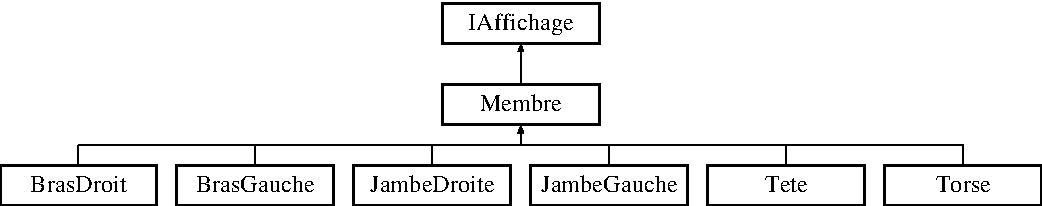
\includegraphics[height=2.772277cm]{class_membre}
\end{center}
\end{figure}
\subsection*{\-Public \-Member \-Functions}
\begin{DoxyCompactItemize}
\item 
int \hyperlink{class_membre_aa4ba3c5babf132246cc84907c37e3738}{get\-Id} ()
\item 
void \hyperlink{class_membre_a4b87bebc56e82f08d4ebdf8bcf773c11}{set\-Id} (int id)
\item 
int \hyperlink{class_membre_a35ddd831b2ca01dd13be213470f2aa65}{get\-P\-D\-V} ()
\item 
void \hyperlink{class_membre_a6b45657cd705c02a6ab5a338d1204f3e}{set\-P\-D\-V} (int p)
\item 
string \hyperlink{class_membre_a6ef6931754fe7ce7e8101bf27bc3ef6a}{get\-Libelle} ()
\item 
void \hyperlink{class_membre_aaffef4990f332871cd1dd9b3fc03a078}{set\-Libelle} (string l)
\item 
\hyperlink{class_equipement}{\-Equipement} \hyperlink{class_membre_a8b57b95b91806ebf6171624ac0a051cb}{get\-Equip} ()
\item 
\hyperlink{class_equipement}{\-Equipement} \hyperlink{class_membre_ab2f78da0480458242168b57cf33e3f7c}{set\-Equip} (\hyperlink{class_equipement}{\-Equipement} e)
\item 
virtual void \hyperlink{class_membre_adc88d8e745a6a46a90722ea2397598c9}{afficher\-Info} ()
\end{DoxyCompactItemize}


\subsection{\-Detailed \-Description}
\-Classe mère \hyperlink{class_membre}{\-Membre}, tous les membres héritent de celle-\/ci \-Implémente l'interface \hyperlink{class_i_affichage}{\-I\-Affichage} 

\subsection{\-Member \-Function \-Documentation}
\hypertarget{class_membre_adc88d8e745a6a46a90722ea2397598c9}{\index{\-Membre@{\-Membre}!afficher\-Info@{afficher\-Info}}
\index{afficher\-Info@{afficher\-Info}!Membre@{\-Membre}}
\subsubsection[{afficher\-Info}]{\setlength{\rightskip}{0pt plus 5cm}virtual void {\bf \-Membre\-::afficher\-Info} (
\begin{DoxyParamCaption}
{}
\end{DoxyParamCaption}
)\hspace{0.3cm}{\ttfamily  \mbox{[}inline, virtual\mbox{]}}}}\label{class_membre_adc88d8e745a6a46a90722ea2397598c9}
\-Procédure d'affichage d'informations, redéfinit celle de l'interface \hyperlink{class_i_affichage}{\-I\-Affichage} 

\-Implements \hyperlink{class_i_affichage_a6123c1cb9079f712b48c0b8bf62e14ef}{\-I\-Affichage}.

\hypertarget{class_membre_a8b57b95b91806ebf6171624ac0a051cb}{\index{\-Membre@{\-Membre}!get\-Equip@{get\-Equip}}
\index{get\-Equip@{get\-Equip}!Membre@{\-Membre}}
\subsubsection[{get\-Equip}]{\setlength{\rightskip}{0pt plus 5cm}{\bf \-Equipement} {\bf \-Membre\-::get\-Equip} (
\begin{DoxyParamCaption}
{}
\end{DoxyParamCaption}
)\hspace{0.3cm}{\ttfamily  \mbox{[}inline\mbox{]}}}}\label{class_membre_a8b57b95b91806ebf6171624ac0a051cb}
\-Accesseur à l'\hyperlink{class_equipement}{\-Equipement} équipé au membre 

\-Reimplemented in \hyperlink{class_bras_droit_a9af72d2589c8c33cc5e5d5e666424957}{\-Bras\-Droit}, \hyperlink{class_bras_gauche_abc90f6e5e9d8fb71f5b7c76cc51d8e48}{\-Bras\-Gauche}, \hyperlink{class_jambe_droite_a4a9ac6e20a14d99b6db5ce2fd0af4aa0}{\-Jambe\-Droite}, \hyperlink{class_jambe_gauche_a050999bb1256f3d409c5708be152344a}{\-Jambe\-Gauche}, \hyperlink{class_tete_ae0e3b91eca717e2e5479f72feaef5b90}{\-Tete}, and \hyperlink{class_torse_aef7412e7ca619d0855aa890d84b4a609}{\-Torse}.

\hypertarget{class_membre_aa4ba3c5babf132246cc84907c37e3738}{\index{\-Membre@{\-Membre}!get\-Id@{get\-Id}}
\index{get\-Id@{get\-Id}!Membre@{\-Membre}}
\subsubsection[{get\-Id}]{\setlength{\rightskip}{0pt plus 5cm}int {\bf \-Membre\-::get\-Id} (
\begin{DoxyParamCaption}
{}
\end{DoxyParamCaption}
)\hspace{0.3cm}{\ttfamily  \mbox{[}inline\mbox{]}}}}\label{class_membre_aa4ba3c5babf132246cc84907c37e3738}
\-Accesseur à l'identifiant du membre 

\-Reimplemented in \hyperlink{class_bras_droit_a9be3f4a94a82e95caa78aaabc6357c2b}{\-Bras\-Droit}, \hyperlink{class_bras_gauche_ad30956e6d1afe81c57ed5545bfe7b0e6}{\-Bras\-Gauche}, \hyperlink{class_jambe_droite_a4dc14c64b239851e5497dc84ca43f6de}{\-Jambe\-Droite}, \hyperlink{class_jambe_gauche_a45630c5110de97c6178e23291aa547f0}{\-Jambe\-Gauche}, \hyperlink{class_tete_a78683bd6baef917ed2db10f1a703b0ac}{\-Tete}, and \hyperlink{class_torse_a58614d9c4ce5021515e9a09d68e3366e}{\-Torse}.

\hypertarget{class_membre_a6ef6931754fe7ce7e8101bf27bc3ef6a}{\index{\-Membre@{\-Membre}!get\-Libelle@{get\-Libelle}}
\index{get\-Libelle@{get\-Libelle}!Membre@{\-Membre}}
\subsubsection[{get\-Libelle}]{\setlength{\rightskip}{0pt plus 5cm}string {\bf \-Membre\-::get\-Libelle} (
\begin{DoxyParamCaption}
{}
\end{DoxyParamCaption}
)\hspace{0.3cm}{\ttfamily  \mbox{[}inline\mbox{]}}}}\label{class_membre_a6ef6931754fe7ce7e8101bf27bc3ef6a}
\-Accesseur au libellé du membre 

\-Reimplemented in \hyperlink{class_bras_droit_a6db96c33ab1043b39127277d1920a63f}{\-Bras\-Droit}, \hyperlink{class_bras_gauche_a0c22b277eae6cf0a0475f02f5037db1f}{\-Bras\-Gauche}, \hyperlink{class_jambe_droite_a236e542d759b7142a42d861612a9ac68}{\-Jambe\-Droite}, \hyperlink{class_jambe_gauche_ab6cacd327fa0c3a9a6084d4d1c52ad51}{\-Jambe\-Gauche}, \hyperlink{class_tete_afb6abc9aae3bd726acbe7f725d6ffa96}{\-Tete}, and \hyperlink{class_torse_a4e2fefc2b6e0486d26b33edcd50d0fb4}{\-Torse}.

\hypertarget{class_membre_a35ddd831b2ca01dd13be213470f2aa65}{\index{\-Membre@{\-Membre}!get\-P\-D\-V@{get\-P\-D\-V}}
\index{get\-P\-D\-V@{get\-P\-D\-V}!Membre@{\-Membre}}
\subsubsection[{get\-P\-D\-V}]{\setlength{\rightskip}{0pt plus 5cm}int {\bf \-Membre\-::get\-P\-D\-V} (
\begin{DoxyParamCaption}
{}
\end{DoxyParamCaption}
)\hspace{0.3cm}{\ttfamily  \mbox{[}inline\mbox{]}}}}\label{class_membre_a35ddd831b2ca01dd13be213470f2aa65}
\-Accesseur au nombre de points de vie du membre 

\-Reimplemented in \hyperlink{class_bras_droit_adddfb977411421906d39f4bd4a35daf1}{\-Bras\-Droit}, \hyperlink{class_bras_gauche_a24954e20008bc8724156731b5450b91f}{\-Bras\-Gauche}, \hyperlink{class_jambe_droite_ab652890a9d08fd39f231dcf9bba48068}{\-Jambe\-Droite}, \hyperlink{class_jambe_gauche_a0012a7b60f3aa32e26dd59f88f7f046f}{\-Jambe\-Gauche}, \hyperlink{class_tete_aa2c9934f7442d9a5e8cb2fc5c050e554}{\-Tete}, and \hyperlink{class_torse_a2f13314c8454f1be93a17ecd3be02408}{\-Torse}.

\hypertarget{class_membre_ab2f78da0480458242168b57cf33e3f7c}{\index{\-Membre@{\-Membre}!set\-Equip@{set\-Equip}}
\index{set\-Equip@{set\-Equip}!Membre@{\-Membre}}
\subsubsection[{set\-Equip}]{\setlength{\rightskip}{0pt plus 5cm}{\bf \-Equipement} {\bf \-Membre\-::set\-Equip} (
\begin{DoxyParamCaption}
\item[{{\bf \-Equipement}}]{e}
\end{DoxyParamCaption}
)\hspace{0.3cm}{\ttfamily  \mbox{[}inline\mbox{]}}}}\label{class_membre_ab2f78da0480458242168b57cf33e3f7c}
\-Mutateur de l'\hyperlink{class_equipement}{\-Equipement} équipé au bras droit 

\-Reimplemented in \hyperlink{class_bras_droit_a726fd8be859bbb27257118ad4c3647dc}{\-Bras\-Droit}, \hyperlink{class_bras_gauche_ad99fefc88e948e61c781a76b4262102b}{\-Bras\-Gauche}, \hyperlink{class_jambe_droite_a1f8dc857d14b8bfb005dcf633e56f8d3}{\-Jambe\-Droite}, \hyperlink{class_jambe_gauche_a6192a0c9850adebf39f9ef14344a8957}{\-Jambe\-Gauche}, \hyperlink{class_tete_a126334fb3e157995becf73c2ba3ff10c}{\-Tete}, and \hyperlink{class_torse_a59c9a4895878649516f5f0622cbce083}{\-Torse}.

\hypertarget{class_membre_a4b87bebc56e82f08d4ebdf8bcf773c11}{\index{\-Membre@{\-Membre}!set\-Id@{set\-Id}}
\index{set\-Id@{set\-Id}!Membre@{\-Membre}}
\subsubsection[{set\-Id}]{\setlength{\rightskip}{0pt plus 5cm}void {\bf \-Membre\-::set\-Id} (
\begin{DoxyParamCaption}
\item[{int}]{id}
\end{DoxyParamCaption}
)\hspace{0.3cm}{\ttfamily  \mbox{[}inline\mbox{]}}}}\label{class_membre_a4b87bebc56e82f08d4ebdf8bcf773c11}
\-Mutateur de l'identifiant du membre 

\-Reimplemented in \hyperlink{class_bras_droit_a156189452ba3e3d037ecca9b21d294cb}{\-Bras\-Droit}, \hyperlink{class_bras_gauche_a0e1accaf25773a48d64f716a6389c33c}{\-Bras\-Gauche}, \hyperlink{class_jambe_droite_ae8840e4f8b4240a24dbdb7311cf49b45}{\-Jambe\-Droite}, \hyperlink{class_jambe_gauche_a2851cb622f0d958c2795bcfe45904209}{\-Jambe\-Gauche}, \hyperlink{class_tete_adf73f2de90a86656810db42e96033858}{\-Tete}, and \hyperlink{class_torse_a797b1977bbc9dd5ab6bb5b6731e3081f}{\-Torse}.

\hypertarget{class_membre_aaffef4990f332871cd1dd9b3fc03a078}{\index{\-Membre@{\-Membre}!set\-Libelle@{set\-Libelle}}
\index{set\-Libelle@{set\-Libelle}!Membre@{\-Membre}}
\subsubsection[{set\-Libelle}]{\setlength{\rightskip}{0pt plus 5cm}void {\bf \-Membre\-::set\-Libelle} (
\begin{DoxyParamCaption}
\item[{string}]{l}
\end{DoxyParamCaption}
)\hspace{0.3cm}{\ttfamily  \mbox{[}inline\mbox{]}}}}\label{class_membre_aaffef4990f332871cd1dd9b3fc03a078}
\-Mutateur du libellé du membre 

\-Reimplemented in \hyperlink{class_bras_droit_adc1f6283b4e00813a099b5cc9b9f8d76}{\-Bras\-Droit}, \hyperlink{class_bras_gauche_a64e26bbb9af48a13f9c4b128ddb74570}{\-Bras\-Gauche}, \hyperlink{class_jambe_droite_ab45dd17c1fcc3de07b55c13a27bf9699}{\-Jambe\-Droite}, \hyperlink{class_jambe_gauche_a5ce53b166f79dbfb157ccc2774dcdbfd}{\-Jambe\-Gauche}, \hyperlink{class_tete_a644eff8bb48835a4e82e848411e30ae8}{\-Tete}, and \hyperlink{class_torse_a89ac35e98847c1f39f8bdb840efddd75}{\-Torse}.

\hypertarget{class_membre_a6b45657cd705c02a6ab5a338d1204f3e}{\index{\-Membre@{\-Membre}!set\-P\-D\-V@{set\-P\-D\-V}}
\index{set\-P\-D\-V@{set\-P\-D\-V}!Membre@{\-Membre}}
\subsubsection[{set\-P\-D\-V}]{\setlength{\rightskip}{0pt plus 5cm}void {\bf \-Membre\-::set\-P\-D\-V} (
\begin{DoxyParamCaption}
\item[{int}]{p}
\end{DoxyParamCaption}
)\hspace{0.3cm}{\ttfamily  \mbox{[}inline\mbox{]}}}}\label{class_membre_a6b45657cd705c02a6ab5a338d1204f3e}
\-Mutateur du nombre de points de vie du membre 

\-Reimplemented in \hyperlink{class_bras_droit_a519053f32bea237a7fe8f7c93d9a0152}{\-Bras\-Droit}, \hyperlink{class_bras_gauche_ac5698d46c3af46fcaaf9a6cd5cd3d495}{\-Bras\-Gauche}, \hyperlink{class_jambe_droite_a720931176b5219a1ef11e5d255910fbe}{\-Jambe\-Droite}, \hyperlink{class_jambe_gauche_af6fc1b58e9f6dd1eeb840c71d1908043}{\-Jambe\-Gauche}, \hyperlink{class_tete_a07df0ae5bc33c6c6c216541046e3995a}{\-Tete}, and \hyperlink{class_torse_a88aeb0ac624296d654a245522e9a7a4c}{\-Torse}.



\-The documentation for this class was generated from the following file\-:\begin{DoxyCompactItemize}
\item 
\-Projet\-P\-O\-O-\/master/\-Membre.\-cpp\end{DoxyCompactItemize}

\hypertarget{class_murmillo}{\section{\-Murmillo \-Class \-Reference}
\label{class_murmillo}\index{\-Murmillo@{\-Murmillo}}
}
\-Inheritance diagram for \-Murmillo\-:\begin{figure}[H]
\begin{center}
\leavevmode
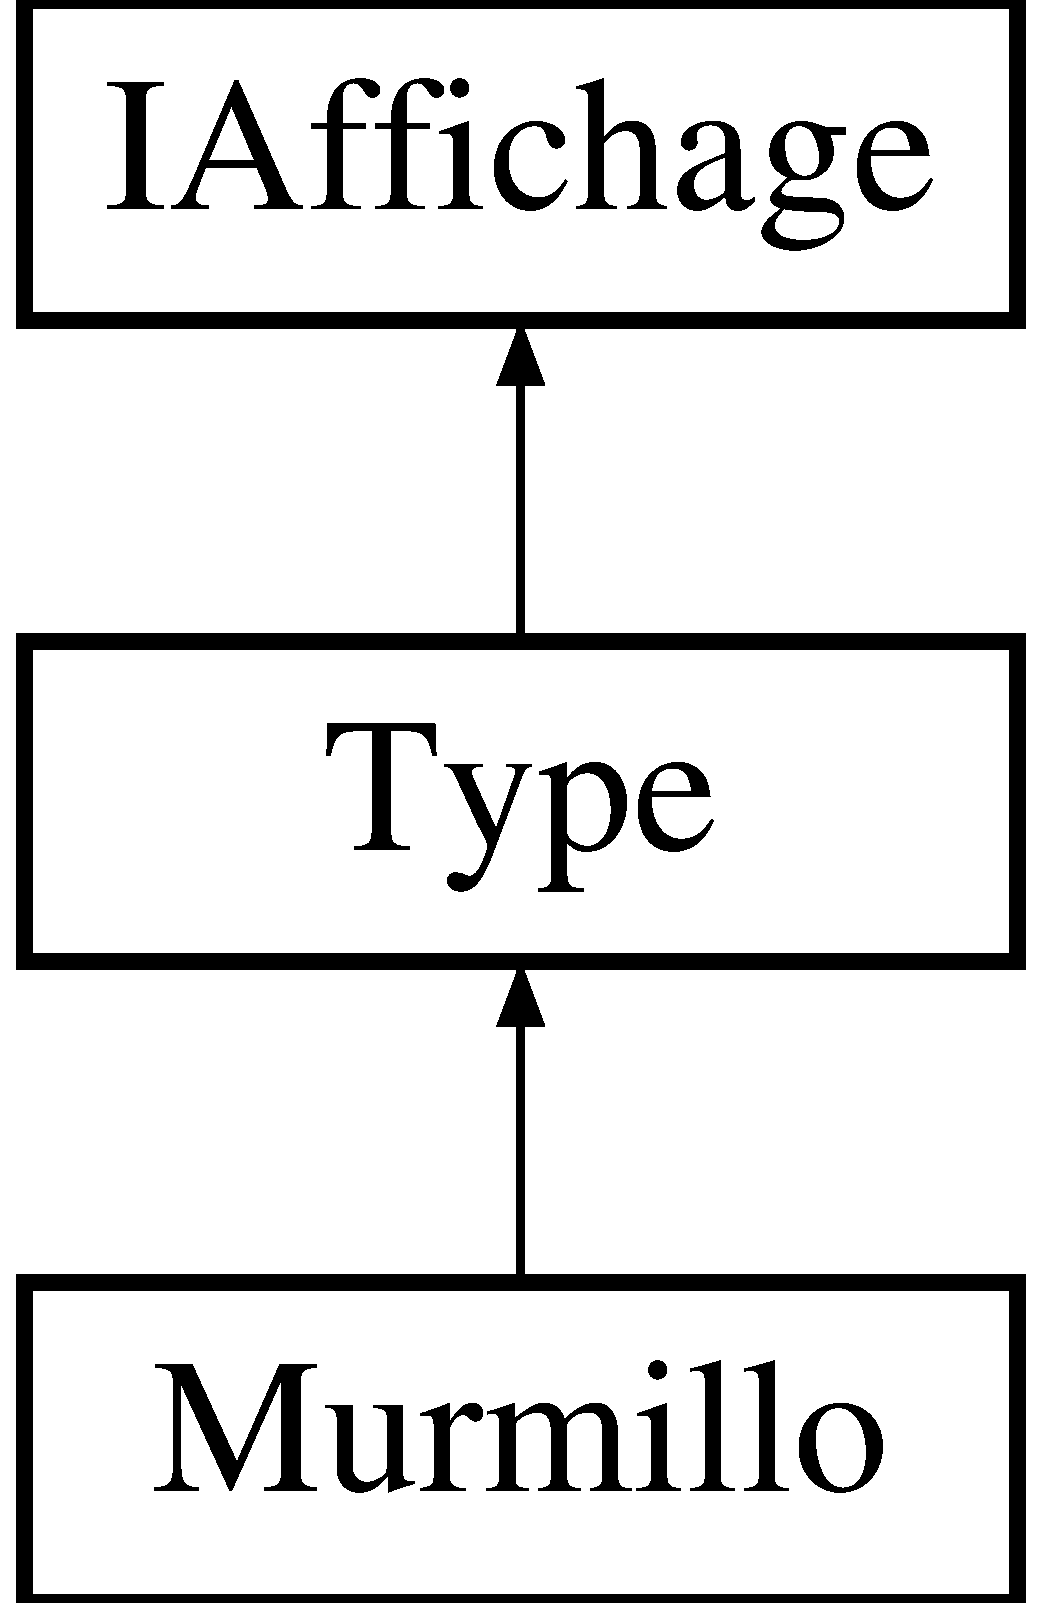
\includegraphics[height=3.000000cm]{class_murmillo}
\end{center}
\end{figure}
\subsection*{\-Public \-Member \-Functions}
\begin{DoxyCompactItemize}
\item 
\hyperlink{class_murmillo_a05592f971d71799fd291347c0a359521}{\-Murmillo} ()
\item 
int \hyperlink{class_murmillo_a90f58f8288899f7ee204b48c4ae99f20}{get\-Id} ()
\item 
void \hyperlink{class_murmillo_a399b7e8cd46c07b076c22b2f34a03d73}{set\-Id} (int id)
\item 
string \hyperlink{class_murmillo_ac7342a7ed268a06e9720c9e19457606a}{get\-Libelle} ()
\item 
void \hyperlink{class_murmillo_a3519f7936494e9f29206899b12647cda}{set\-Libelle} (string l)
\end{DoxyCompactItemize}


\subsection{\-Detailed \-Description}
\-Classe \hyperlink{class_murmillo}{\-Murmillo}, hérite de \hyperlink{class_type}{\-Type} 

\subsection{\-Constructor \& \-Destructor \-Documentation}
\hypertarget{class_murmillo_a05592f971d71799fd291347c0a359521}{\index{\-Murmillo@{\-Murmillo}!\-Murmillo@{\-Murmillo}}
\index{\-Murmillo@{\-Murmillo}!Murmillo@{\-Murmillo}}
\subsubsection[{\-Murmillo}]{\setlength{\rightskip}{0pt plus 5cm}{\bf \-Murmillo\-::\-Murmillo} (
\begin{DoxyParamCaption}
{}
\end{DoxyParamCaption}
)\hspace{0.3cm}{\ttfamily  \mbox{[}inline\mbox{]}}}}\label{class_murmillo_a05592f971d71799fd291347c0a359521}
\-Constructeur explicite initialisant les variables du type 

\subsection{\-Member \-Function \-Documentation}
\hypertarget{class_murmillo_a90f58f8288899f7ee204b48c4ae99f20}{\index{\-Murmillo@{\-Murmillo}!get\-Id@{get\-Id}}
\index{get\-Id@{get\-Id}!Murmillo@{\-Murmillo}}
\subsubsection[{get\-Id}]{\setlength{\rightskip}{0pt plus 5cm}int {\bf \-Murmillo\-::get\-Id} (
\begin{DoxyParamCaption}
{}
\end{DoxyParamCaption}
)\hspace{0.3cm}{\ttfamily  \mbox{[}inline\mbox{]}}}}\label{class_murmillo_a90f58f8288899f7ee204b48c4ae99f20}
\-Accesseur à l'identifiant du type 

\-Reimplemented from \hyperlink{class_type_aba890fe7677f58f7135ec0cfe1b7c926}{\-Type}.

\hypertarget{class_murmillo_ac7342a7ed268a06e9720c9e19457606a}{\index{\-Murmillo@{\-Murmillo}!get\-Libelle@{get\-Libelle}}
\index{get\-Libelle@{get\-Libelle}!Murmillo@{\-Murmillo}}
\subsubsection[{get\-Libelle}]{\setlength{\rightskip}{0pt plus 5cm}string {\bf \-Murmillo\-::get\-Libelle} (
\begin{DoxyParamCaption}
{}
\end{DoxyParamCaption}
)\hspace{0.3cm}{\ttfamily  \mbox{[}inline\mbox{]}}}}\label{class_murmillo_ac7342a7ed268a06e9720c9e19457606a}
\-Accesseur au libellé du type 

\-Reimplemented from \hyperlink{class_type_a38a529eb6a80a3d3cb801996cc9f41f0}{\-Type}.

\hypertarget{class_murmillo_a399b7e8cd46c07b076c22b2f34a03d73}{\index{\-Murmillo@{\-Murmillo}!set\-Id@{set\-Id}}
\index{set\-Id@{set\-Id}!Murmillo@{\-Murmillo}}
\subsubsection[{set\-Id}]{\setlength{\rightskip}{0pt plus 5cm}void {\bf \-Murmillo\-::set\-Id} (
\begin{DoxyParamCaption}
\item[{int}]{id}
\end{DoxyParamCaption}
)\hspace{0.3cm}{\ttfamily  \mbox{[}inline\mbox{]}}}}\label{class_murmillo_a399b7e8cd46c07b076c22b2f34a03d73}
\-Mutateur de l'identifiant du type 

\-Reimplemented from \hyperlink{class_type_ab9b8158dca9be6184557382ec98ec4f7}{\-Type}.

\hypertarget{class_murmillo_a3519f7936494e9f29206899b12647cda}{\index{\-Murmillo@{\-Murmillo}!set\-Libelle@{set\-Libelle}}
\index{set\-Libelle@{set\-Libelle}!Murmillo@{\-Murmillo}}
\subsubsection[{set\-Libelle}]{\setlength{\rightskip}{0pt plus 5cm}void {\bf \-Murmillo\-::set\-Libelle} (
\begin{DoxyParamCaption}
\item[{string}]{l}
\end{DoxyParamCaption}
)\hspace{0.3cm}{\ttfamily  \mbox{[}inline\mbox{]}}}}\label{class_murmillo_a3519f7936494e9f29206899b12647cda}
\-Mutateur du libellé du type 

\-Reimplemented from \hyperlink{class_type_af475df921624fe329aaa6b19bd1ed2e1}{\-Type}.



\-The documentation for this class was generated from the following file\-:\begin{DoxyCompactItemize}
\item 
\-Projet\-P\-O\-O-\/master/\-Murmillo.\-cpp\end{DoxyCompactItemize}

\hypertarget{class_personnage}{\section{\-Personnage \-Class \-Reference}
\label{class_personnage}\index{\-Personnage@{\-Personnage}}
}
\-Inheritance diagram for \-Personnage\-:\begin{figure}[H]
\begin{center}
\leavevmode
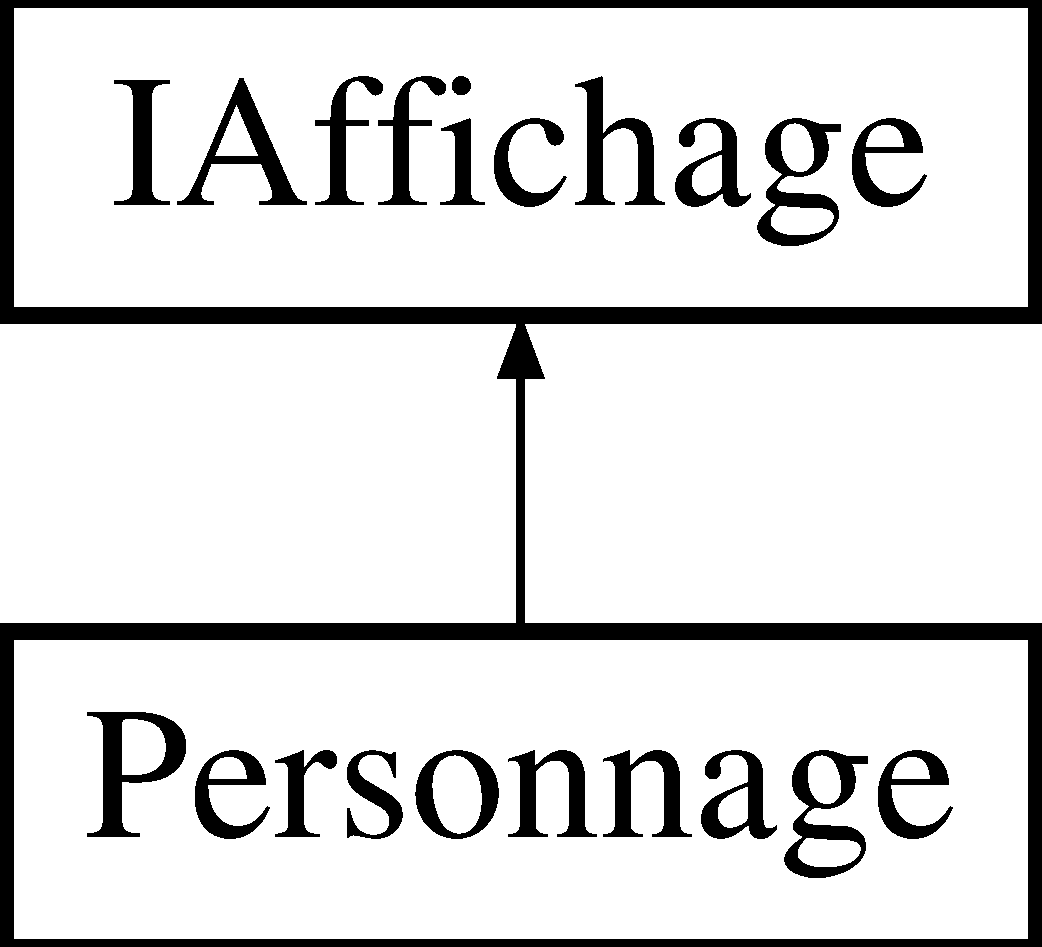
\includegraphics[height=2.000000cm]{class_personnage}
\end{center}
\end{figure}
\subsection*{\-Public \-Types}
\begin{DoxyCompactItemize}
\item 
enum {\bfseries types} \{ \*
{\bfseries \-D\-I\-M\-A\-C\-H\-A\-E\-R\-U\-S} =  1, 
{\bfseries \-R\-E\-T\-I\-A\-R\-I\-U\-S} =  2, 
{\bfseries \-M\-U\-R\-M\-I\-L\-L\-O} =  3, 
{\bfseries \-V\-E\-L\-I\-T\-E} =  4, 
\*
{\bfseries \-T\-H\-R\-A\-E\-X} =  5, 
{\bfseries \-S\-E\-C\-U\-T\-O\-R} =  6
 \}
\item 
enum {\bfseries etats} \{ {\bfseries \-P\-O\-I\-S\-O\-N} =  1, 
{\bfseries \-B\-L\-E\-E\-D} =  2, 
{\bfseries \-R\-O\-O\-T} =  3
 \}
\end{DoxyCompactItemize}
\subsection*{\-Public \-Member \-Functions}
\begin{DoxyCompactItemize}
\item 
\hypertarget{class_personnage_a962f03c014911e25449829891f1e2d15}{{\bfseries \-Personnage} (int id, string nom, int type)}\label{class_personnage_a962f03c014911e25449829891f1e2d15}

\item 
\hypertarget{class_personnage_a24fbf035171564c8cb2abff10642d73c}{int {\bfseries get\-Id} ()}\label{class_personnage_a24fbf035171564c8cb2abff10642d73c}

\item 
\hypertarget{class_personnage_a5eaaea57f901cf1f04c1ee4752f03007}{void {\bfseries set\-Id} (int id)}\label{class_personnage_a5eaaea57f901cf1f04c1ee4752f03007}

\item 
\hypertarget{class_personnage_a8e5dab03a028a1c04b692f737c495979}{int {\bfseries get\-P\-D\-V} ()}\label{class_personnage_a8e5dab03a028a1c04b692f737c495979}

\item 
\hypertarget{class_personnage_ada4855cf75754881b579a3a84aba2f47}{void {\bfseries set\-P\-D\-V} (int p)}\label{class_personnage_ada4855cf75754881b579a3a84aba2f47}

\item 
\hypertarget{class_personnage_a519301399a9bee1557858aa50a04a85a}{string {\bfseries get\-Nom} ()}\label{class_personnage_a519301399a9bee1557858aa50a04a85a}

\item 
\hypertarget{class_personnage_a73b26b1b2f225f10fba5e1c294f47f8a}{void {\bfseries set\-Nom} (string l)}\label{class_personnage_a73b26b1b2f225f10fba5e1c294f47f8a}

\item 
\hypertarget{class_personnage_adc6cc2d57410d41817814775eae0fc7b}{\hyperlink{class_type}{\-Type} $\ast$ {\bfseries get\-Type} ()}\label{class_personnage_adc6cc2d57410d41817814775eae0fc7b}

\item 
\hypertarget{class_personnage_aab567206193ab8e53a6ab8a1a972123f}{int {\bfseries get\-Index\-Last\-Effet} ()}\label{class_personnage_aab567206193ab8e53a6ab8a1a972123f}

\item 
\hypertarget{class_personnage_a11d434b9150ee0bd6487f34b6afbdf44}{void {\bfseries set\-Index\-Last\-Effet} (int e)}\label{class_personnage_a11d434b9150ee0bd6487f34b6afbdf44}

\item 
\hypertarget{class_personnage_a30747012401c2f14d40cbf70da549a50}{void {\bfseries ajouter\-Membres} ()}\label{class_personnage_a30747012401c2f14d40cbf70da549a50}

\item 
\hypertarget{class_personnage_a8025dcfd3f7c0284aae99527267e13c9}{void {\bfseries ajouter\-Effet\-Actif} (int effet)}\label{class_personnage_a8025dcfd3f7c0284aae99527267e13c9}

\item 
void \hyperlink{class_personnage_a79ce4d8f13bc64471c553a32f2bb0e2d}{afficher\-Info} ()
\item 
\hypertarget{class_personnage_ab6d8d089b1e19738e898cf5b346e0bb6}{void {\bfseries prendre\-Coup} (int id\-Membre\-Vise)}\label{class_personnage_ab6d8d089b1e19738e898cf5b346e0bb6}

\end{DoxyCompactItemize}


\subsection{\-Detailed \-Description}
\-Classe \hyperlink{class_personnage}{\-Personnage} \-Implémente l'interface \hyperlink{class_i_affichage}{\-I\-Affichage} 

\subsection{\-Member \-Function \-Documentation}
\hypertarget{class_personnage_a79ce4d8f13bc64471c553a32f2bb0e2d}{\index{\-Personnage@{\-Personnage}!afficher\-Info@{afficher\-Info}}
\index{afficher\-Info@{afficher\-Info}!Personnage@{\-Personnage}}
\subsubsection[{afficher\-Info}]{\setlength{\rightskip}{0pt plus 5cm}void {\bf \-Personnage\-::afficher\-Info} (
\begin{DoxyParamCaption}
{}
\end{DoxyParamCaption}
)\hspace{0.3cm}{\ttfamily  \mbox{[}inline, virtual\mbox{]}}}}\label{class_personnage_a79ce4d8f13bc64471c553a32f2bb0e2d}
\-Méthode d'affichage à redéfinir par chaque classe utilisatrice 

\-Implements \hyperlink{class_i_affichage_a6123c1cb9079f712b48c0b8bf62e14ef}{\-I\-Affichage}.



\-The documentation for this class was generated from the following file\-:\begin{DoxyCompactItemize}
\item 
\-Projet\-P\-O\-O-\/master/\-Personnage.\-cpp\end{DoxyCompactItemize}

\hypertarget{class_retiarius}{\section{\-Retiarius \-Class \-Reference}
\label{class_retiarius}\index{\-Retiarius@{\-Retiarius}}
}
\-Inheritance diagram for \-Retiarius\-:\begin{figure}[H]
\begin{center}
\leavevmode
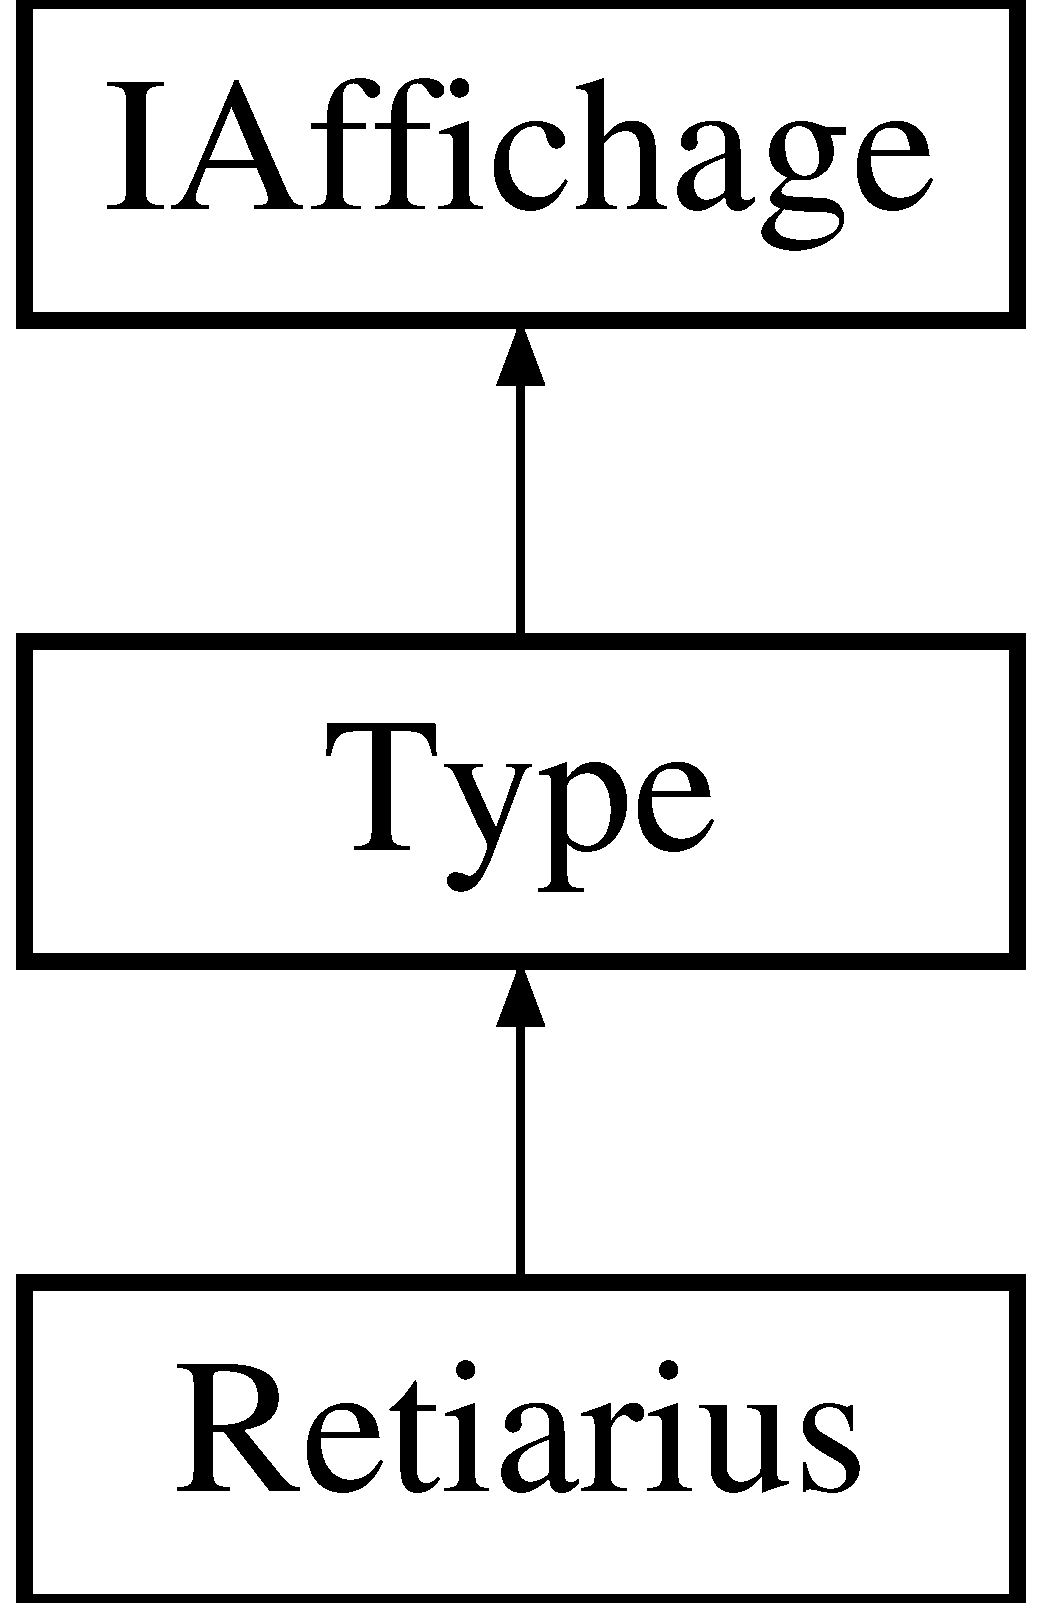
\includegraphics[height=3.000000cm]{class_retiarius}
\end{center}
\end{figure}
\subsection*{\-Public \-Member \-Functions}
\begin{DoxyCompactItemize}
\item 
\hyperlink{class_retiarius_a61abe7207c15167c759a2260059f3918}{\-Retiarius} ()
\item 
int \hyperlink{class_retiarius_af5b641eab15c0a2c82ecfb3aefd0ec53}{get\-Id} ()
\item 
void \hyperlink{class_retiarius_a9d96e3aee6a81c635123b42645cc61f6}{set\-Id} (int id)
\item 
string \hyperlink{class_retiarius_a46a096b0223b86b1ff90fab62da23d4c}{get\-Libelle} ()
\item 
void \hyperlink{class_retiarius_a952a9490820bfe1494fe69e44631a04c}{set\-Libelle} (string l)
\end{DoxyCompactItemize}


\subsection{\-Detailed \-Description}
\-Classe \hyperlink{class_retiarius}{\-Retiarius}, hérite de \hyperlink{class_type}{\-Type} 

\subsection{\-Constructor \& \-Destructor \-Documentation}
\hypertarget{class_retiarius_a61abe7207c15167c759a2260059f3918}{\index{\-Retiarius@{\-Retiarius}!\-Retiarius@{\-Retiarius}}
\index{\-Retiarius@{\-Retiarius}!Retiarius@{\-Retiarius}}
\subsubsection[{\-Retiarius}]{\setlength{\rightskip}{0pt plus 5cm}{\bf \-Retiarius\-::\-Retiarius} (
\begin{DoxyParamCaption}
{}
\end{DoxyParamCaption}
)\hspace{0.3cm}{\ttfamily  \mbox{[}inline\mbox{]}}}}\label{class_retiarius_a61abe7207c15167c759a2260059f3918}
\-Constructeur explicite initialisant les variables du type 

\subsection{\-Member \-Function \-Documentation}
\hypertarget{class_retiarius_af5b641eab15c0a2c82ecfb3aefd0ec53}{\index{\-Retiarius@{\-Retiarius}!get\-Id@{get\-Id}}
\index{get\-Id@{get\-Id}!Retiarius@{\-Retiarius}}
\subsubsection[{get\-Id}]{\setlength{\rightskip}{0pt plus 5cm}int {\bf \-Retiarius\-::get\-Id} (
\begin{DoxyParamCaption}
{}
\end{DoxyParamCaption}
)\hspace{0.3cm}{\ttfamily  \mbox{[}inline\mbox{]}}}}\label{class_retiarius_af5b641eab15c0a2c82ecfb3aefd0ec53}
\-Accesseur à l'identifiant du type 

\-Reimplemented from \hyperlink{class_type_aba890fe7677f58f7135ec0cfe1b7c926}{\-Type}.

\hypertarget{class_retiarius_a46a096b0223b86b1ff90fab62da23d4c}{\index{\-Retiarius@{\-Retiarius}!get\-Libelle@{get\-Libelle}}
\index{get\-Libelle@{get\-Libelle}!Retiarius@{\-Retiarius}}
\subsubsection[{get\-Libelle}]{\setlength{\rightskip}{0pt plus 5cm}string {\bf \-Retiarius\-::get\-Libelle} (
\begin{DoxyParamCaption}
{}
\end{DoxyParamCaption}
)\hspace{0.3cm}{\ttfamily  \mbox{[}inline\mbox{]}}}}\label{class_retiarius_a46a096b0223b86b1ff90fab62da23d4c}
\-Accesseur au libellé du type 

\-Reimplemented from \hyperlink{class_type_a38a529eb6a80a3d3cb801996cc9f41f0}{\-Type}.

\hypertarget{class_retiarius_a9d96e3aee6a81c635123b42645cc61f6}{\index{\-Retiarius@{\-Retiarius}!set\-Id@{set\-Id}}
\index{set\-Id@{set\-Id}!Retiarius@{\-Retiarius}}
\subsubsection[{set\-Id}]{\setlength{\rightskip}{0pt plus 5cm}void {\bf \-Retiarius\-::set\-Id} (
\begin{DoxyParamCaption}
\item[{int}]{id}
\end{DoxyParamCaption}
)\hspace{0.3cm}{\ttfamily  \mbox{[}inline\mbox{]}}}}\label{class_retiarius_a9d96e3aee6a81c635123b42645cc61f6}
\-Mutateur de l'identifiant du type 

\-Reimplemented from \hyperlink{class_type_ab9b8158dca9be6184557382ec98ec4f7}{\-Type}.

\hypertarget{class_retiarius_a952a9490820bfe1494fe69e44631a04c}{\index{\-Retiarius@{\-Retiarius}!set\-Libelle@{set\-Libelle}}
\index{set\-Libelle@{set\-Libelle}!Retiarius@{\-Retiarius}}
\subsubsection[{set\-Libelle}]{\setlength{\rightskip}{0pt plus 5cm}void {\bf \-Retiarius\-::set\-Libelle} (
\begin{DoxyParamCaption}
\item[{string}]{l}
\end{DoxyParamCaption}
)\hspace{0.3cm}{\ttfamily  \mbox{[}inline\mbox{]}}}}\label{class_retiarius_a952a9490820bfe1494fe69e44631a04c}
\-Mutateur du libellé du type 

\-Reimplemented from \hyperlink{class_type_af475df921624fe329aaa6b19bd1ed2e1}{\-Type}.



\-The documentation for this class was generated from the following file\-:\begin{DoxyCompactItemize}
\item 
\-Projet\-P\-O\-O-\/master/\-Retiarius.\-cpp\end{DoxyCompactItemize}

\hypertarget{class_saignement}{\section{\-Saignement \-Class \-Reference}
\label{class_saignement}\index{\-Saignement@{\-Saignement}}
}
\-Inheritance diagram for \-Saignement\-:\begin{figure}[H]
\begin{center}
\leavevmode
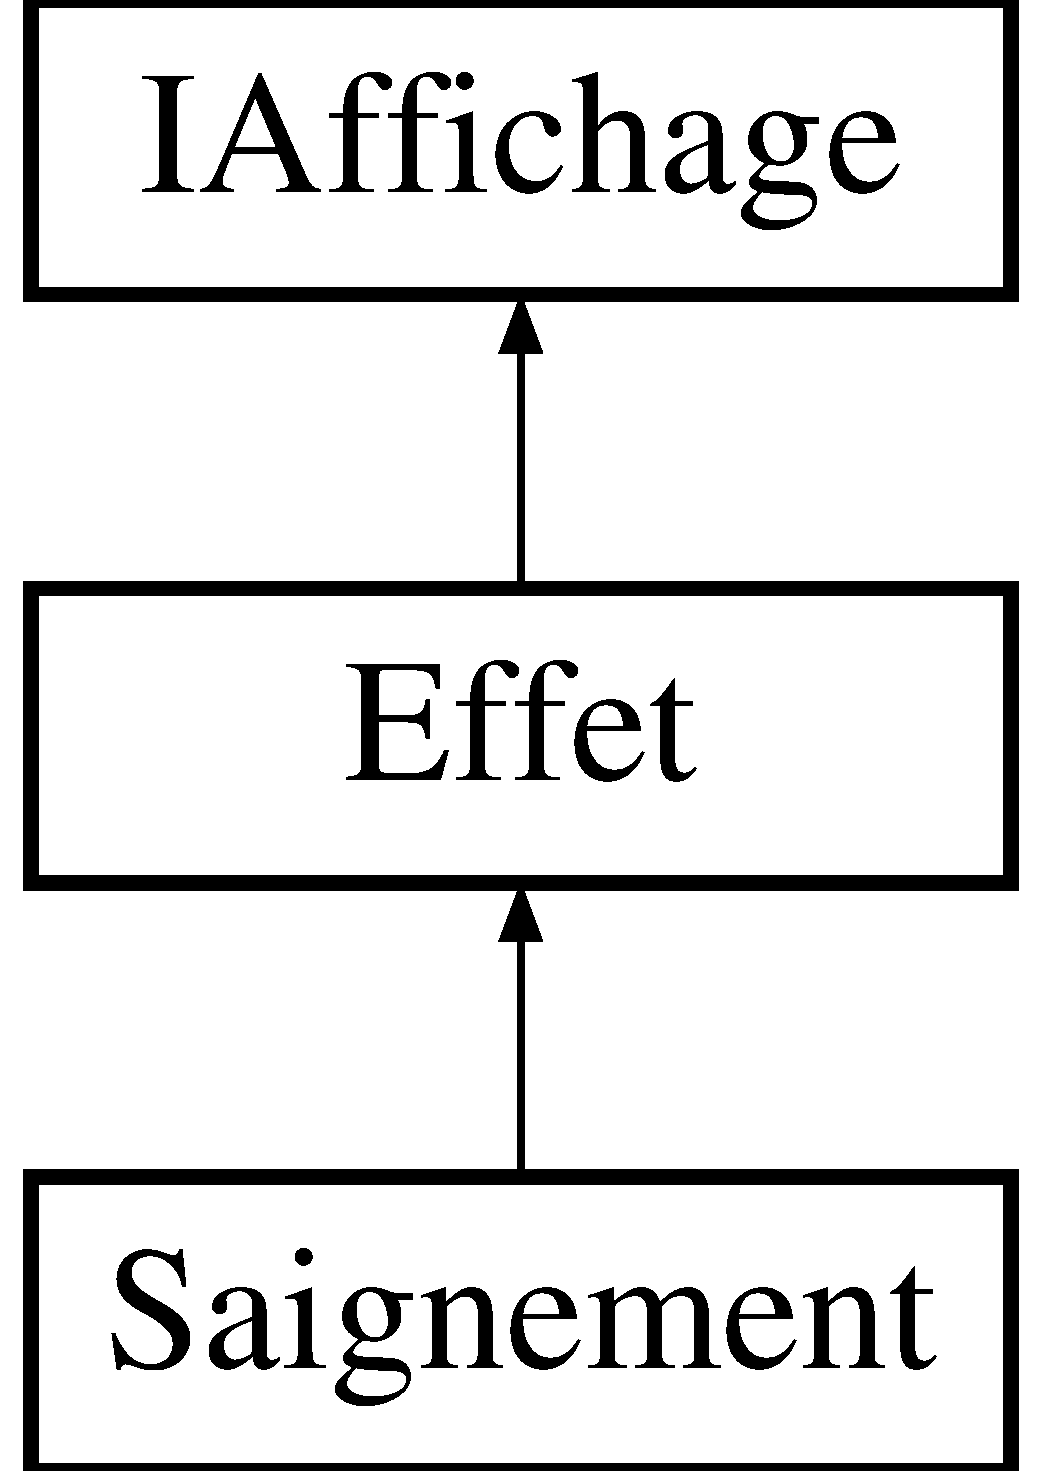
\includegraphics[height=3.000000cm]{class_saignement}
\end{center}
\end{figure}
\subsection*{\-Public \-Member \-Functions}
\begin{DoxyCompactItemize}
\item 
\hyperlink{class_saignement_a83d7b835d237439cf350507765dbf8cf}{\-Saignement} ()
\item 
int \hyperlink{class_saignement_a57ccf17cade8c253a7ee99e7f816eb10}{get\-Id} ()
\item 
void \hyperlink{class_saignement_af9d66877c7e2aff769b4bc48f4bb82e4}{set\-Id} (int id)
\item 
string \hyperlink{class_saignement_aca2c045c2faa9384b6cf25ec3c11af28}{get\-Libelle} ()
\item 
void \hyperlink{class_saignement_a2c9f7ffb81aa8848564389580c4f7112}{set\-Libelle} (string l)
\item 
int \hyperlink{class_saignement_a498bf00562314e4094be4004e5bc653a}{get\-Nb\-Tours\-Max} ()
\item 
void \hyperlink{class_saignement_ae31708c65c109f4169d1e79fca31eade}{set\-Nb\-Tours\-Max} (int n)
\item 
int \hyperlink{class_saignement_a16b32f7a90575e7d80695bcc8a5a03c8}{get\-Val\-Deg} ()
\item 
void \hyperlink{class_saignement_a5b3fcda8a30588355f7cb5699131c8a0}{set\-Val\-Deg} (int v)
\end{DoxyCompactItemize}


\subsection{\-Detailed \-Description}
\-Classe \hyperlink{class_saignement}{\-Saignement}, hérite d'\hyperlink{class_effet}{\-Effet} 

\subsection{\-Constructor \& \-Destructor \-Documentation}
\hypertarget{class_saignement_a83d7b835d237439cf350507765dbf8cf}{\index{\-Saignement@{\-Saignement}!\-Saignement@{\-Saignement}}
\index{\-Saignement@{\-Saignement}!Saignement@{\-Saignement}}
\subsubsection[{\-Saignement}]{\setlength{\rightskip}{0pt plus 5cm}{\bf \-Saignement\-::\-Saignement} (
\begin{DoxyParamCaption}
{}
\end{DoxyParamCaption}
)\hspace{0.3cm}{\ttfamily  \mbox{[}inline\mbox{]}}}}\label{class_saignement_a83d7b835d237439cf350507765dbf8cf}
\-Constructeur explicite initialisant les variables de l'effet 

\subsection{\-Member \-Function \-Documentation}
\hypertarget{class_saignement_a57ccf17cade8c253a7ee99e7f816eb10}{\index{\-Saignement@{\-Saignement}!get\-Id@{get\-Id}}
\index{get\-Id@{get\-Id}!Saignement@{\-Saignement}}
\subsubsection[{get\-Id}]{\setlength{\rightskip}{0pt plus 5cm}int {\bf \-Saignement\-::get\-Id} (
\begin{DoxyParamCaption}
{}
\end{DoxyParamCaption}
)\hspace{0.3cm}{\ttfamily  \mbox{[}inline\mbox{]}}}}\label{class_saignement_a57ccf17cade8c253a7ee99e7f816eb10}
\-Accesseur à l'identifiant de l'effet 

\-Reimplemented from \hyperlink{class_effet_a509c2d845776b583280b4418585d9ec2}{\-Effet}.

\hypertarget{class_saignement_aca2c045c2faa9384b6cf25ec3c11af28}{\index{\-Saignement@{\-Saignement}!get\-Libelle@{get\-Libelle}}
\index{get\-Libelle@{get\-Libelle}!Saignement@{\-Saignement}}
\subsubsection[{get\-Libelle}]{\setlength{\rightskip}{0pt plus 5cm}string {\bf \-Saignement\-::get\-Libelle} (
\begin{DoxyParamCaption}
{}
\end{DoxyParamCaption}
)\hspace{0.3cm}{\ttfamily  \mbox{[}inline\mbox{]}}}}\label{class_saignement_aca2c045c2faa9384b6cf25ec3c11af28}
\-Accesseur au libellé de l'effet 

\-Reimplemented from \hyperlink{class_effet_a1817f59e4c17c91103ae4031868dfd97}{\-Effet}.

\hypertarget{class_saignement_a498bf00562314e4094be4004e5bc653a}{\index{\-Saignement@{\-Saignement}!get\-Nb\-Tours\-Max@{get\-Nb\-Tours\-Max}}
\index{get\-Nb\-Tours\-Max@{get\-Nb\-Tours\-Max}!Saignement@{\-Saignement}}
\subsubsection[{get\-Nb\-Tours\-Max}]{\setlength{\rightskip}{0pt plus 5cm}int {\bf \-Saignement\-::get\-Nb\-Tours\-Max} (
\begin{DoxyParamCaption}
{}
\end{DoxyParamCaption}
)\hspace{0.3cm}{\ttfamily  \mbox{[}inline\mbox{]}}}}\label{class_saignement_a498bf00562314e4094be4004e5bc653a}
\-Accesseur de la durée maximale, en tours, de l'effet 

\-Reimplemented from \hyperlink{class_effet_ae98c2a33fcd29629e3c7cd6e8ab8fcd8}{\-Effet}.

\hypertarget{class_saignement_a16b32f7a90575e7d80695bcc8a5a03c8}{\index{\-Saignement@{\-Saignement}!get\-Val\-Deg@{get\-Val\-Deg}}
\index{get\-Val\-Deg@{get\-Val\-Deg}!Saignement@{\-Saignement}}
\subsubsection[{get\-Val\-Deg}]{\setlength{\rightskip}{0pt plus 5cm}int {\bf \-Saignement\-::get\-Val\-Deg} (
\begin{DoxyParamCaption}
{}
\end{DoxyParamCaption}
)\hspace{0.3cm}{\ttfamily  \mbox{[}inline\mbox{]}}}}\label{class_saignement_a16b32f7a90575e7d80695bcc8a5a03c8}
\-Accesseur à la valeur de dégâts de l'effet \hypertarget{class_saignement_af9d66877c7e2aff769b4bc48f4bb82e4}{\index{\-Saignement@{\-Saignement}!set\-Id@{set\-Id}}
\index{set\-Id@{set\-Id}!Saignement@{\-Saignement}}
\subsubsection[{set\-Id}]{\setlength{\rightskip}{0pt plus 5cm}void {\bf \-Saignement\-::set\-Id} (
\begin{DoxyParamCaption}
\item[{int}]{id}
\end{DoxyParamCaption}
)\hspace{0.3cm}{\ttfamily  \mbox{[}inline\mbox{]}}}}\label{class_saignement_af9d66877c7e2aff769b4bc48f4bb82e4}
\-Mutateur de l'identifiant de l'effet 

\-Reimplemented from \hyperlink{class_effet_a1e880a5364a175e90dae7cbfdc103e02}{\-Effet}.

\hypertarget{class_saignement_a2c9f7ffb81aa8848564389580c4f7112}{\index{\-Saignement@{\-Saignement}!set\-Libelle@{set\-Libelle}}
\index{set\-Libelle@{set\-Libelle}!Saignement@{\-Saignement}}
\subsubsection[{set\-Libelle}]{\setlength{\rightskip}{0pt plus 5cm}void {\bf \-Saignement\-::set\-Libelle} (
\begin{DoxyParamCaption}
\item[{string}]{l}
\end{DoxyParamCaption}
)\hspace{0.3cm}{\ttfamily  \mbox{[}inline\mbox{]}}}}\label{class_saignement_a2c9f7ffb81aa8848564389580c4f7112}
\-Mutateur du libellé de l'effet 

\-Reimplemented from \hyperlink{class_effet_a8470c57c7d69b4023c5230cdca79631d}{\-Effet}.

\hypertarget{class_saignement_ae31708c65c109f4169d1e79fca31eade}{\index{\-Saignement@{\-Saignement}!set\-Nb\-Tours\-Max@{set\-Nb\-Tours\-Max}}
\index{set\-Nb\-Tours\-Max@{set\-Nb\-Tours\-Max}!Saignement@{\-Saignement}}
\subsubsection[{set\-Nb\-Tours\-Max}]{\setlength{\rightskip}{0pt plus 5cm}void {\bf \-Saignement\-::set\-Nb\-Tours\-Max} (
\begin{DoxyParamCaption}
\item[{int}]{n}
\end{DoxyParamCaption}
)\hspace{0.3cm}{\ttfamily  \mbox{[}inline\mbox{]}}}}\label{class_saignement_ae31708c65c109f4169d1e79fca31eade}
\-Mutateur de la durée maximale, en tours, de l'effet 

\-Reimplemented from \hyperlink{class_effet_a12959d98a93ca835aedd8b7ed84e5a61}{\-Effet}.

\hypertarget{class_saignement_a5b3fcda8a30588355f7cb5699131c8a0}{\index{\-Saignement@{\-Saignement}!set\-Val\-Deg@{set\-Val\-Deg}}
\index{set\-Val\-Deg@{set\-Val\-Deg}!Saignement@{\-Saignement}}
\subsubsection[{set\-Val\-Deg}]{\setlength{\rightskip}{0pt plus 5cm}void {\bf \-Saignement\-::set\-Val\-Deg} (
\begin{DoxyParamCaption}
\item[{int}]{v}
\end{DoxyParamCaption}
)\hspace{0.3cm}{\ttfamily  \mbox{[}inline\mbox{]}}}}\label{class_saignement_a5b3fcda8a30588355f7cb5699131c8a0}
\-Mutateur de la valeur de dégâts de l'effet 

\-The documentation for this class was generated from the following file\-:\begin{DoxyCompactItemize}
\item 
\-Projet\-P\-O\-O-\/master/\-Saignement.\-cpp\end{DoxyCompactItemize}

\hypertarget{class_secutor}{\section{\-Secutor \-Class \-Reference}
\label{class_secutor}\index{\-Secutor@{\-Secutor}}
}
\-Inheritance diagram for \-Secutor\-:\begin{figure}[H]
\begin{center}
\leavevmode
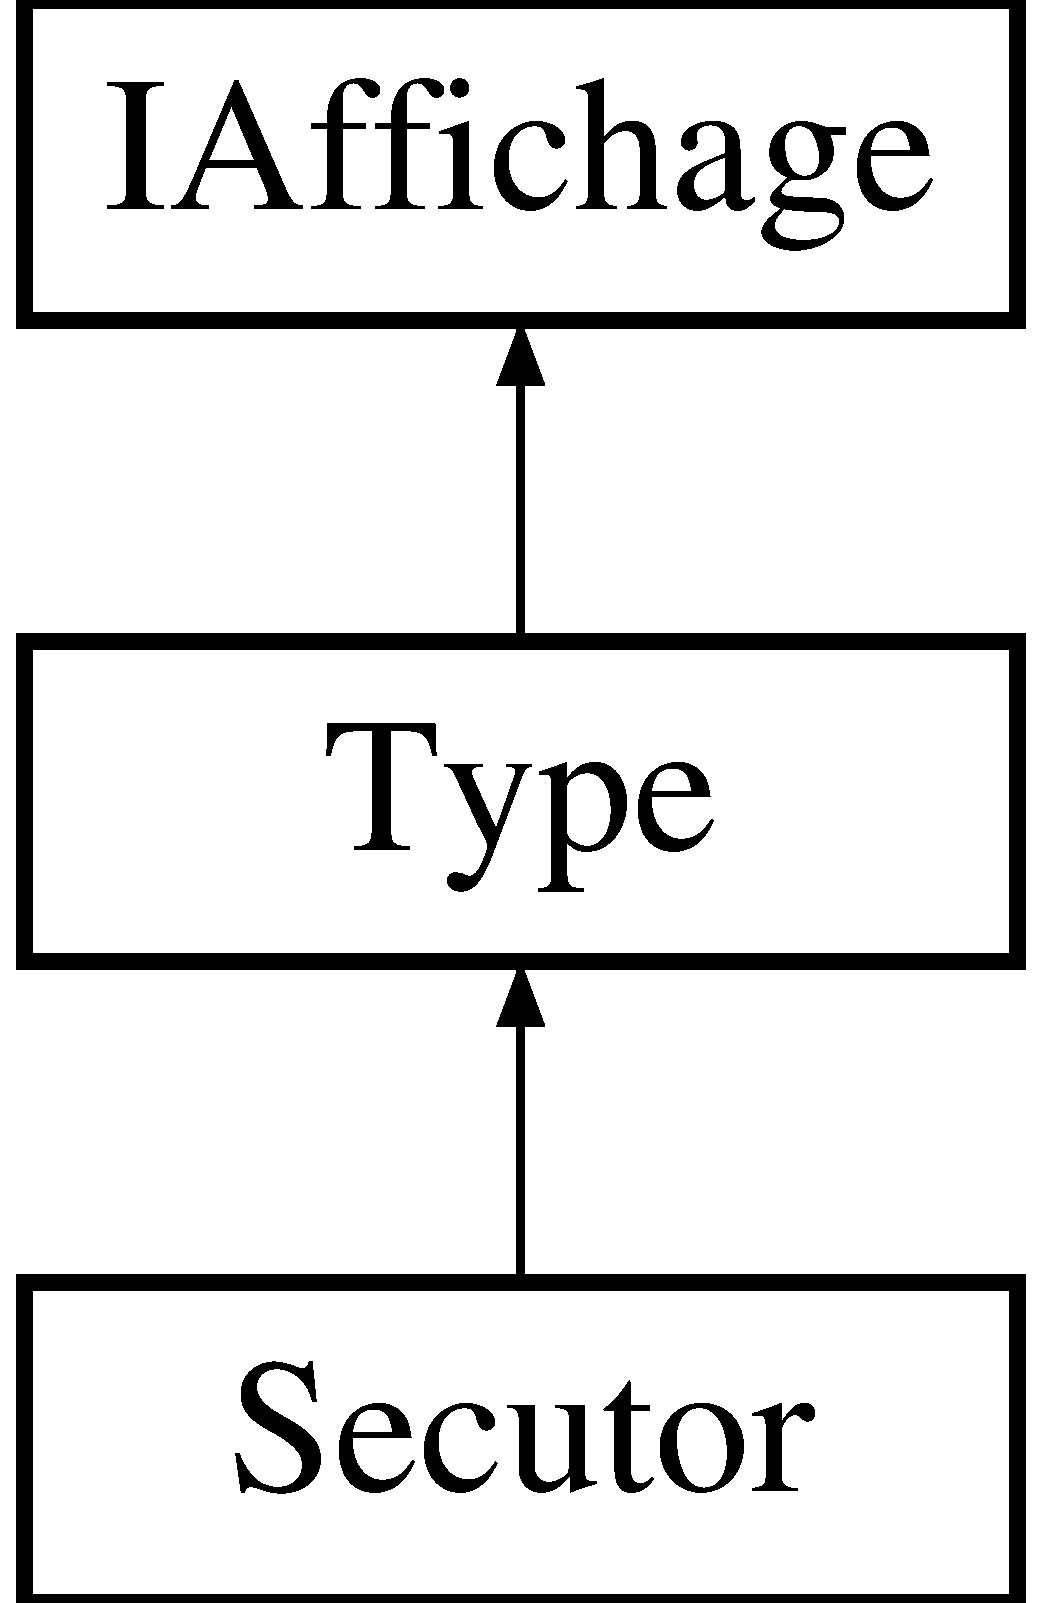
\includegraphics[height=3.000000cm]{class_secutor}
\end{center}
\end{figure}
\subsection*{\-Public \-Member \-Functions}
\begin{DoxyCompactItemize}
\item 
\hyperlink{class_secutor_a2196c86cf9cd5d0727a92129d7caf769}{\-Secutor} ()
\item 
int \hyperlink{class_secutor_ad1dddc99e73479adcba390c52f7fd3a9}{get\-Id} ()
\item 
void \hyperlink{class_secutor_a469886024806f30aad616f170f29593f}{set\-Id} (int id)
\item 
string \hyperlink{class_secutor_a36403dd64d3717d786ed96559768122a}{get\-Libelle} ()
\item 
void \hyperlink{class_secutor_a5746d934d179b165684f540b1edd4327}{set\-Libelle} (string l)
\end{DoxyCompactItemize}


\subsection{\-Detailed \-Description}
\-Classe \hyperlink{class_secutor}{\-Secutor}, hérite de \hyperlink{class_type}{\-Type} 

\subsection{\-Constructor \& \-Destructor \-Documentation}
\hypertarget{class_secutor_a2196c86cf9cd5d0727a92129d7caf769}{\index{\-Secutor@{\-Secutor}!\-Secutor@{\-Secutor}}
\index{\-Secutor@{\-Secutor}!Secutor@{\-Secutor}}
\subsubsection[{\-Secutor}]{\setlength{\rightskip}{0pt plus 5cm}{\bf \-Secutor\-::\-Secutor} (
\begin{DoxyParamCaption}
{}
\end{DoxyParamCaption}
)\hspace{0.3cm}{\ttfamily  \mbox{[}inline\mbox{]}}}}\label{class_secutor_a2196c86cf9cd5d0727a92129d7caf769}
\-Constructeur explicite initialisant les variables du type 

\subsection{\-Member \-Function \-Documentation}
\hypertarget{class_secutor_ad1dddc99e73479adcba390c52f7fd3a9}{\index{\-Secutor@{\-Secutor}!get\-Id@{get\-Id}}
\index{get\-Id@{get\-Id}!Secutor@{\-Secutor}}
\subsubsection[{get\-Id}]{\setlength{\rightskip}{0pt plus 5cm}int {\bf \-Secutor\-::get\-Id} (
\begin{DoxyParamCaption}
{}
\end{DoxyParamCaption}
)\hspace{0.3cm}{\ttfamily  \mbox{[}inline\mbox{]}}}}\label{class_secutor_ad1dddc99e73479adcba390c52f7fd3a9}
\-Accesseur à l'identifiant du type 

\-Reimplemented from \hyperlink{class_type_aba890fe7677f58f7135ec0cfe1b7c926}{\-Type}.

\hypertarget{class_secutor_a36403dd64d3717d786ed96559768122a}{\index{\-Secutor@{\-Secutor}!get\-Libelle@{get\-Libelle}}
\index{get\-Libelle@{get\-Libelle}!Secutor@{\-Secutor}}
\subsubsection[{get\-Libelle}]{\setlength{\rightskip}{0pt plus 5cm}string {\bf \-Secutor\-::get\-Libelle} (
\begin{DoxyParamCaption}
{}
\end{DoxyParamCaption}
)\hspace{0.3cm}{\ttfamily  \mbox{[}inline\mbox{]}}}}\label{class_secutor_a36403dd64d3717d786ed96559768122a}
\-Accesseur au libellé du type 

\-Reimplemented from \hyperlink{class_type_a38a529eb6a80a3d3cb801996cc9f41f0}{\-Type}.

\hypertarget{class_secutor_a469886024806f30aad616f170f29593f}{\index{\-Secutor@{\-Secutor}!set\-Id@{set\-Id}}
\index{set\-Id@{set\-Id}!Secutor@{\-Secutor}}
\subsubsection[{set\-Id}]{\setlength{\rightskip}{0pt plus 5cm}void {\bf \-Secutor\-::set\-Id} (
\begin{DoxyParamCaption}
\item[{int}]{id}
\end{DoxyParamCaption}
)\hspace{0.3cm}{\ttfamily  \mbox{[}inline\mbox{]}}}}\label{class_secutor_a469886024806f30aad616f170f29593f}
\-Mutateur de l'identifiant du type 

\-Reimplemented from \hyperlink{class_type_ab9b8158dca9be6184557382ec98ec4f7}{\-Type}.

\hypertarget{class_secutor_a5746d934d179b165684f540b1edd4327}{\index{\-Secutor@{\-Secutor}!set\-Libelle@{set\-Libelle}}
\index{set\-Libelle@{set\-Libelle}!Secutor@{\-Secutor}}
\subsubsection[{set\-Libelle}]{\setlength{\rightskip}{0pt plus 5cm}void {\bf \-Secutor\-::set\-Libelle} (
\begin{DoxyParamCaption}
\item[{string}]{l}
\end{DoxyParamCaption}
)\hspace{0.3cm}{\ttfamily  \mbox{[}inline\mbox{]}}}}\label{class_secutor_a5746d934d179b165684f540b1edd4327}
\-Mutateur du libellé du type 

\-Reimplemented from \hyperlink{class_type_af475df921624fe329aaa6b19bd1ed2e1}{\-Type}.



\-The documentation for this class was generated from the following file\-:\begin{DoxyCompactItemize}
\item 
\-Projet\-P\-O\-O-\/master/\-Secutor.\-cpp\end{DoxyCompactItemize}

\hypertarget{class_sica}{\section{\-Sica \-Class \-Reference}
\label{class_sica}\index{\-Sica@{\-Sica}}
}
\-Inheritance diagram for \-Sica\-:\begin{figure}[H]
\begin{center}
\leavevmode
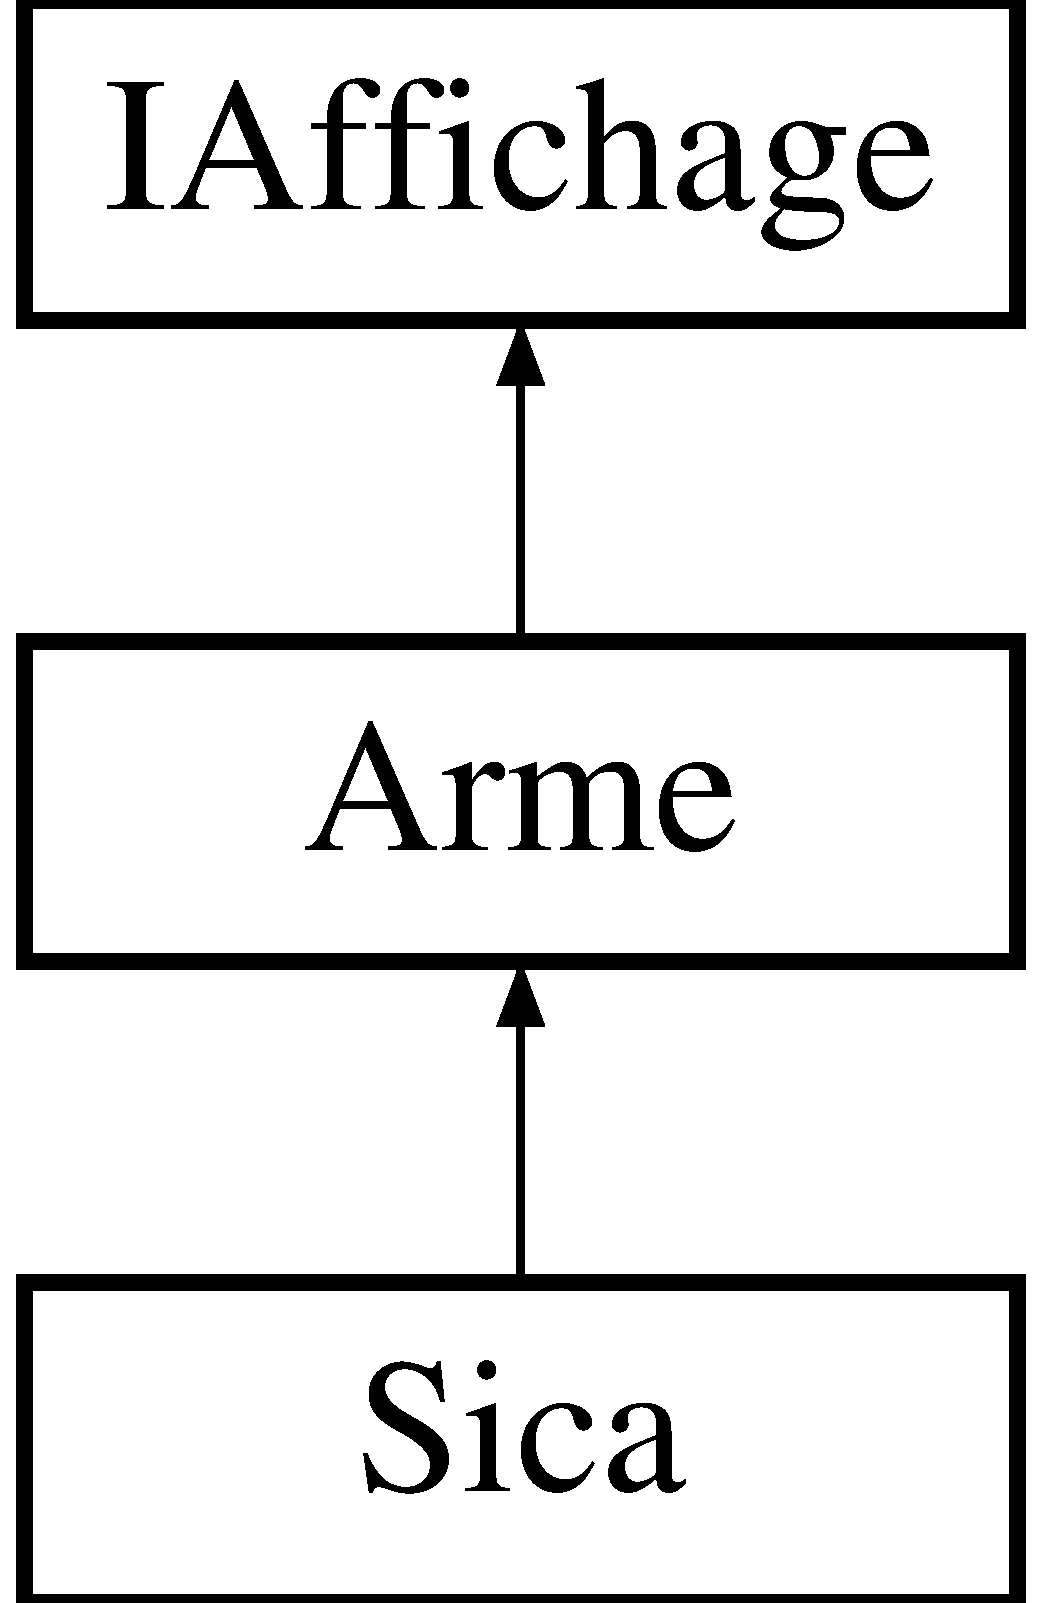
\includegraphics[height=3.000000cm]{class_sica}
\end{center}
\end{figure}
\subsection*{\-Public \-Member \-Functions}
\begin{DoxyCompactItemize}
\item 
\hyperlink{class_sica_af50ede4978099d6462d4baadc8db2c14}{\-Sica} ()
\item 
int \hyperlink{class_sica_a97460a3554bc4bc42b332fd0c267ee32}{get\-Id} ()
\item 
void \hyperlink{class_sica_a990b41f36bb50618e7911ebaa959c343}{set\-Id} (int id)
\item 
string \hyperlink{class_sica_ad7f3cf89e918b618c0ad76f40132e65e}{get\-Libelle} ()
\item 
void \hyperlink{class_sica_ab4ade5608a0321ef4fe1bc9b5ee85e17}{set\-Libelle} (string l)
\item 
int \hyperlink{class_sica_a32189d76350d2924e7b1af6518ee77cf}{get\-Val\-Deg} ()
\item 
void \hyperlink{class_sica_ac26ce3e730ece92a66cd809dbfb4bddf}{set\-Val\-Deg} (int v)
\end{DoxyCompactItemize}


\subsection{\-Detailed \-Description}
\-Classe \hyperlink{class_sica}{\-Sica}, hérite d'\hyperlink{class_arme}{\-Arme} 

\subsection{\-Constructor \& \-Destructor \-Documentation}
\hypertarget{class_sica_af50ede4978099d6462d4baadc8db2c14}{\index{\-Sica@{\-Sica}!\-Sica@{\-Sica}}
\index{\-Sica@{\-Sica}!Sica@{\-Sica}}
\subsubsection[{\-Sica}]{\setlength{\rightskip}{0pt plus 5cm}{\bf \-Sica\-::\-Sica} (
\begin{DoxyParamCaption}
{}
\end{DoxyParamCaption}
)\hspace{0.3cm}{\ttfamily  \mbox{[}inline\mbox{]}}}}\label{class_sica_af50ede4978099d6462d4baadc8db2c14}
\-Constructeur explicite initialisant les variables du sica 

\subsection{\-Member \-Function \-Documentation}
\hypertarget{class_sica_a97460a3554bc4bc42b332fd0c267ee32}{\index{\-Sica@{\-Sica}!get\-Id@{get\-Id}}
\index{get\-Id@{get\-Id}!Sica@{\-Sica}}
\subsubsection[{get\-Id}]{\setlength{\rightskip}{0pt plus 5cm}int {\bf \-Sica\-::get\-Id} (
\begin{DoxyParamCaption}
{}
\end{DoxyParamCaption}
)\hspace{0.3cm}{\ttfamily  \mbox{[}inline\mbox{]}}}}\label{class_sica_a97460a3554bc4bc42b332fd0c267ee32}
\-Accesseur à l'identifiant du sica 

\-Reimplemented from \hyperlink{class_arme_a6c957484697d9ad38ab1ed4361f3b8f4}{\-Arme}.

\hypertarget{class_sica_ad7f3cf89e918b618c0ad76f40132e65e}{\index{\-Sica@{\-Sica}!get\-Libelle@{get\-Libelle}}
\index{get\-Libelle@{get\-Libelle}!Sica@{\-Sica}}
\subsubsection[{get\-Libelle}]{\setlength{\rightskip}{0pt plus 5cm}string {\bf \-Sica\-::get\-Libelle} (
\begin{DoxyParamCaption}
{}
\end{DoxyParamCaption}
)\hspace{0.3cm}{\ttfamily  \mbox{[}inline\mbox{]}}}}\label{class_sica_ad7f3cf89e918b618c0ad76f40132e65e}
\-Accesseur au libellé de l'arme 

\-Reimplemented from \hyperlink{class_arme_a5e43d33d0e14da19fb37dc497474135b}{\-Arme}.

\hypertarget{class_sica_a32189d76350d2924e7b1af6518ee77cf}{\index{\-Sica@{\-Sica}!get\-Val\-Deg@{get\-Val\-Deg}}
\index{get\-Val\-Deg@{get\-Val\-Deg}!Sica@{\-Sica}}
\subsubsection[{get\-Val\-Deg}]{\setlength{\rightskip}{0pt plus 5cm}int {\bf \-Sica\-::get\-Val\-Deg} (
\begin{DoxyParamCaption}
{}
\end{DoxyParamCaption}
)\hspace{0.3cm}{\ttfamily  \mbox{[}inline\mbox{]}}}}\label{class_sica_a32189d76350d2924e7b1af6518ee77cf}
\-Accesseur à la valeur de dégâts du sica \hypertarget{class_sica_a990b41f36bb50618e7911ebaa959c343}{\index{\-Sica@{\-Sica}!set\-Id@{set\-Id}}
\index{set\-Id@{set\-Id}!Sica@{\-Sica}}
\subsubsection[{set\-Id}]{\setlength{\rightskip}{0pt plus 5cm}void {\bf \-Sica\-::set\-Id} (
\begin{DoxyParamCaption}
\item[{int}]{id}
\end{DoxyParamCaption}
)\hspace{0.3cm}{\ttfamily  \mbox{[}inline\mbox{]}}}}\label{class_sica_a990b41f36bb50618e7911ebaa959c343}
\-Mutateur de l'identifiant du sica 

\-Reimplemented from \hyperlink{class_arme_a332699f4c7b2dab9e38fccfddba7275b}{\-Arme}.

\hypertarget{class_sica_ab4ade5608a0321ef4fe1bc9b5ee85e17}{\index{\-Sica@{\-Sica}!set\-Libelle@{set\-Libelle}}
\index{set\-Libelle@{set\-Libelle}!Sica@{\-Sica}}
\subsubsection[{set\-Libelle}]{\setlength{\rightskip}{0pt plus 5cm}void {\bf \-Sica\-::set\-Libelle} (
\begin{DoxyParamCaption}
\item[{string}]{l}
\end{DoxyParamCaption}
)\hspace{0.3cm}{\ttfamily  \mbox{[}inline\mbox{]}}}}\label{class_sica_ab4ade5608a0321ef4fe1bc9b5ee85e17}
\-Mutateur du libellé de l'arme 

\-Reimplemented from \hyperlink{class_arme_ab38eebb032ab6773678ee40f152df6dd}{\-Arme}.

\hypertarget{class_sica_ac26ce3e730ece92a66cd809dbfb4bddf}{\index{\-Sica@{\-Sica}!set\-Val\-Deg@{set\-Val\-Deg}}
\index{set\-Val\-Deg@{set\-Val\-Deg}!Sica@{\-Sica}}
\subsubsection[{set\-Val\-Deg}]{\setlength{\rightskip}{0pt plus 5cm}void {\bf \-Sica\-::set\-Val\-Deg} (
\begin{DoxyParamCaption}
\item[{int}]{v}
\end{DoxyParamCaption}
)\hspace{0.3cm}{\ttfamily  \mbox{[}inline\mbox{]}}}}\label{class_sica_ac26ce3e730ece92a66cd809dbfb4bddf}
\-Mutateur de la valeur de dégâts du sica 

\-The documentation for this class was generated from the following file\-:\begin{DoxyCompactItemize}
\item 
\-Projet\-P\-O\-O-\/master/\-Sica.\-cpp\end{DoxyCompactItemize}

\hypertarget{class_spaliere_bras_armure}{\section{\-Spaliere\-Bras\-Armure \-Class \-Reference}
\label{class_spaliere_bras_armure}\index{\-Spaliere\-Bras\-Armure@{\-Spaliere\-Bras\-Armure}}
}
\-Inheritance diagram for \-Spaliere\-Bras\-Armure\-:\begin{figure}[H]
\begin{center}
\leavevmode
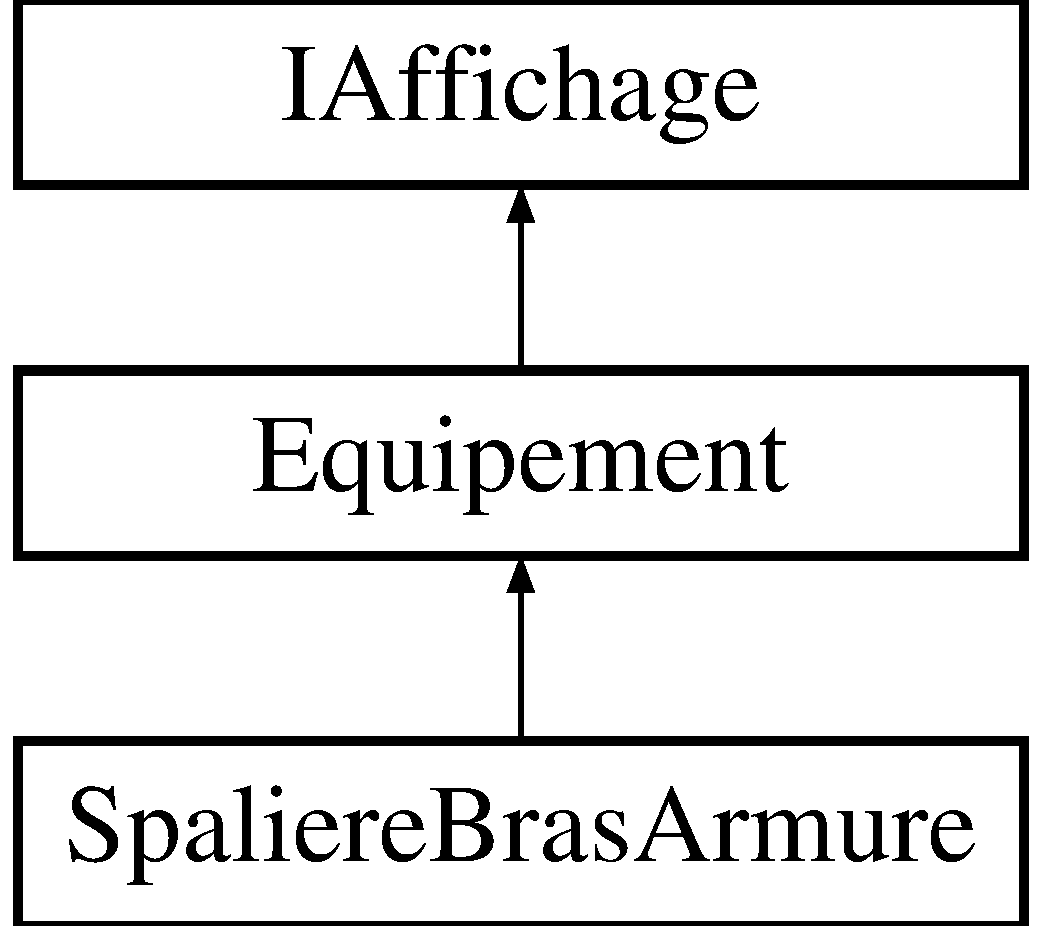
\includegraphics[height=3.000000cm]{class_spaliere_bras_armure}
\end{center}
\end{figure}
\subsection*{\-Public \-Member \-Functions}
\begin{DoxyCompactItemize}
\item 
\hyperlink{class_spaliere_bras_armure_abf26fad2754d5ece7b738597b86a77d6}{\-Spaliere\-Bras\-Armure} ()
\item 
int \hyperlink{class_spaliere_bras_armure_aced30cd7ce6d4b4cf0276ebd174164b5}{get\-Id} ()
\item 
void \hyperlink{class_spaliere_bras_armure_ab7de03f7a7056ec768400a3d6073f3ef}{set\-Id} (int id)
\item 
string \hyperlink{class_spaliere_bras_armure_a5cccfb1ec9c35ce6ff193b956922ac0b}{get\-Libelle} ()
\item 
void \hyperlink{class_spaliere_bras_armure_a8c7a3990c4cc8e4f01157b686d2b4f0a}{set\-Libelle} (string l)
\item 
int \hyperlink{class_spaliere_bras_armure_af0f4b0c780083719852fcff96bc0083f}{get\-Val\-Def} ()
\item 
void \hyperlink{class_spaliere_bras_armure_ac7c03928bacb86e6ff9a6743ed46cb16}{set\-Val\-Def} (int v)
\end{DoxyCompactItemize}


\subsection{\-Detailed \-Description}
\-Classe \hyperlink{class_spaliere_bras_armure}{\-Spaliere\-Bras\-Armure}, hérite d'\hyperlink{class_equipement}{\-Equipement} 

\subsection{\-Constructor \& \-Destructor \-Documentation}
\hypertarget{class_spaliere_bras_armure_abf26fad2754d5ece7b738597b86a77d6}{\index{\-Spaliere\-Bras\-Armure@{\-Spaliere\-Bras\-Armure}!\-Spaliere\-Bras\-Armure@{\-Spaliere\-Bras\-Armure}}
\index{\-Spaliere\-Bras\-Armure@{\-Spaliere\-Bras\-Armure}!SpaliereBrasArmure@{\-Spaliere\-Bras\-Armure}}
\subsubsection[{\-Spaliere\-Bras\-Armure}]{\setlength{\rightskip}{0pt plus 5cm}{\bf \-Spaliere\-Bras\-Armure\-::\-Spaliere\-Bras\-Armure} (
\begin{DoxyParamCaption}
{}
\end{DoxyParamCaption}
)\hspace{0.3cm}{\ttfamily  \mbox{[}inline\mbox{]}}}}\label{class_spaliere_bras_armure_abf26fad2754d5ece7b738597b86a77d6}
\-Constructeur explicite initialisant les variables de la spaulière/bras d'armure 

\subsection{\-Member \-Function \-Documentation}
\hypertarget{class_spaliere_bras_armure_aced30cd7ce6d4b4cf0276ebd174164b5}{\index{\-Spaliere\-Bras\-Armure@{\-Spaliere\-Bras\-Armure}!get\-Id@{get\-Id}}
\index{get\-Id@{get\-Id}!SpaliereBrasArmure@{\-Spaliere\-Bras\-Armure}}
\subsubsection[{get\-Id}]{\setlength{\rightskip}{0pt plus 5cm}int {\bf \-Spaliere\-Bras\-Armure\-::get\-Id} (
\begin{DoxyParamCaption}
{}
\end{DoxyParamCaption}
)\hspace{0.3cm}{\ttfamily  \mbox{[}inline\mbox{]}}}}\label{class_spaliere_bras_armure_aced30cd7ce6d4b4cf0276ebd174164b5}
\-Accesseur à l'identifiant de la spalière/bras d'armure 

\-Reimplemented from \hyperlink{class_equipement_abc38941f5a9deed943b7a83ce69539c3}{\-Equipement}.

\hypertarget{class_spaliere_bras_armure_a5cccfb1ec9c35ce6ff193b956922ac0b}{\index{\-Spaliere\-Bras\-Armure@{\-Spaliere\-Bras\-Armure}!get\-Libelle@{get\-Libelle}}
\index{get\-Libelle@{get\-Libelle}!SpaliereBrasArmure@{\-Spaliere\-Bras\-Armure}}
\subsubsection[{get\-Libelle}]{\setlength{\rightskip}{0pt plus 5cm}string {\bf \-Spaliere\-Bras\-Armure\-::get\-Libelle} (
\begin{DoxyParamCaption}
{}
\end{DoxyParamCaption}
)\hspace{0.3cm}{\ttfamily  \mbox{[}inline\mbox{]}}}}\label{class_spaliere_bras_armure_a5cccfb1ec9c35ce6ff193b956922ac0b}
\-Accesseur au libellé de l'équipement 

\-Reimplemented from \hyperlink{class_equipement_ab00ec565966647bf6edeb1a9df430aa6}{\-Equipement}.

\hypertarget{class_spaliere_bras_armure_af0f4b0c780083719852fcff96bc0083f}{\index{\-Spaliere\-Bras\-Armure@{\-Spaliere\-Bras\-Armure}!get\-Val\-Def@{get\-Val\-Def}}
\index{get\-Val\-Def@{get\-Val\-Def}!SpaliereBrasArmure@{\-Spaliere\-Bras\-Armure}}
\subsubsection[{get\-Val\-Def}]{\setlength{\rightskip}{0pt plus 5cm}int {\bf \-Spaliere\-Bras\-Armure\-::get\-Val\-Def} (
\begin{DoxyParamCaption}
{}
\end{DoxyParamCaption}
)\hspace{0.3cm}{\ttfamily  \mbox{[}inline\mbox{]}}}}\label{class_spaliere_bras_armure_af0f4b0c780083719852fcff96bc0083f}
\-Accesseur à la valeur de défense de la spalière/bras d'armure 

\-Reimplemented from \hyperlink{class_equipement_a7b3003f4da24a94bfec94555e35e772c}{\-Equipement}.

\hypertarget{class_spaliere_bras_armure_ab7de03f7a7056ec768400a3d6073f3ef}{\index{\-Spaliere\-Bras\-Armure@{\-Spaliere\-Bras\-Armure}!set\-Id@{set\-Id}}
\index{set\-Id@{set\-Id}!SpaliereBrasArmure@{\-Spaliere\-Bras\-Armure}}
\subsubsection[{set\-Id}]{\setlength{\rightskip}{0pt plus 5cm}void {\bf \-Spaliere\-Bras\-Armure\-::set\-Id} (
\begin{DoxyParamCaption}
\item[{int}]{id}
\end{DoxyParamCaption}
)\hspace{0.3cm}{\ttfamily  \mbox{[}inline\mbox{]}}}}\label{class_spaliere_bras_armure_ab7de03f7a7056ec768400a3d6073f3ef}
\-Mutateur de l'identifiant de la spalière/bras d'armure 

\-Reimplemented from \hyperlink{class_equipement_a98208826ad05cbc38211e9f70bd908c5}{\-Equipement}.

\hypertarget{class_spaliere_bras_armure_a8c7a3990c4cc8e4f01157b686d2b4f0a}{\index{\-Spaliere\-Bras\-Armure@{\-Spaliere\-Bras\-Armure}!set\-Libelle@{set\-Libelle}}
\index{set\-Libelle@{set\-Libelle}!SpaliereBrasArmure@{\-Spaliere\-Bras\-Armure}}
\subsubsection[{set\-Libelle}]{\setlength{\rightskip}{0pt plus 5cm}void {\bf \-Spaliere\-Bras\-Armure\-::set\-Libelle} (
\begin{DoxyParamCaption}
\item[{string}]{l}
\end{DoxyParamCaption}
)\hspace{0.3cm}{\ttfamily  \mbox{[}inline\mbox{]}}}}\label{class_spaliere_bras_armure_a8c7a3990c4cc8e4f01157b686d2b4f0a}
\-Mutateur du libellé de l'équipement 

\-Reimplemented from \hyperlink{class_equipement_aea246b68c747bd5ec84ca8ce4c4c7b40}{\-Equipement}.

\hypertarget{class_spaliere_bras_armure_ac7c03928bacb86e6ff9a6743ed46cb16}{\index{\-Spaliere\-Bras\-Armure@{\-Spaliere\-Bras\-Armure}!set\-Val\-Def@{set\-Val\-Def}}
\index{set\-Val\-Def@{set\-Val\-Def}!SpaliereBrasArmure@{\-Spaliere\-Bras\-Armure}}
\subsubsection[{set\-Val\-Def}]{\setlength{\rightskip}{0pt plus 5cm}void {\bf \-Spaliere\-Bras\-Armure\-::set\-Val\-Def} (
\begin{DoxyParamCaption}
\item[{int}]{v}
\end{DoxyParamCaption}
)\hspace{0.3cm}{\ttfamily  \mbox{[}inline\mbox{]}}}}\label{class_spaliere_bras_armure_ac7c03928bacb86e6ff9a6743ed46cb16}
\-Mutateur de la valeur de défense de la spalière/bras d'armure 

\-Reimplemented from \hyperlink{class_equipement_ad9940c901b3a96b91c5c3f24713face5}{\-Equipement}.



\-The documentation for this class was generated from the following file\-:\begin{DoxyCompactItemize}
\item 
\-Projet\-P\-O\-O-\/master/\-Spaliere\-Bras\-Armure.\-cpp\end{DoxyCompactItemize}

\hypertarget{class_tete}{\section{\-Tete \-Class \-Reference}
\label{class_tete}\index{\-Tete@{\-Tete}}
}
\-Inheritance diagram for \-Tete\-:\begin{figure}[H]
\begin{center}
\leavevmode
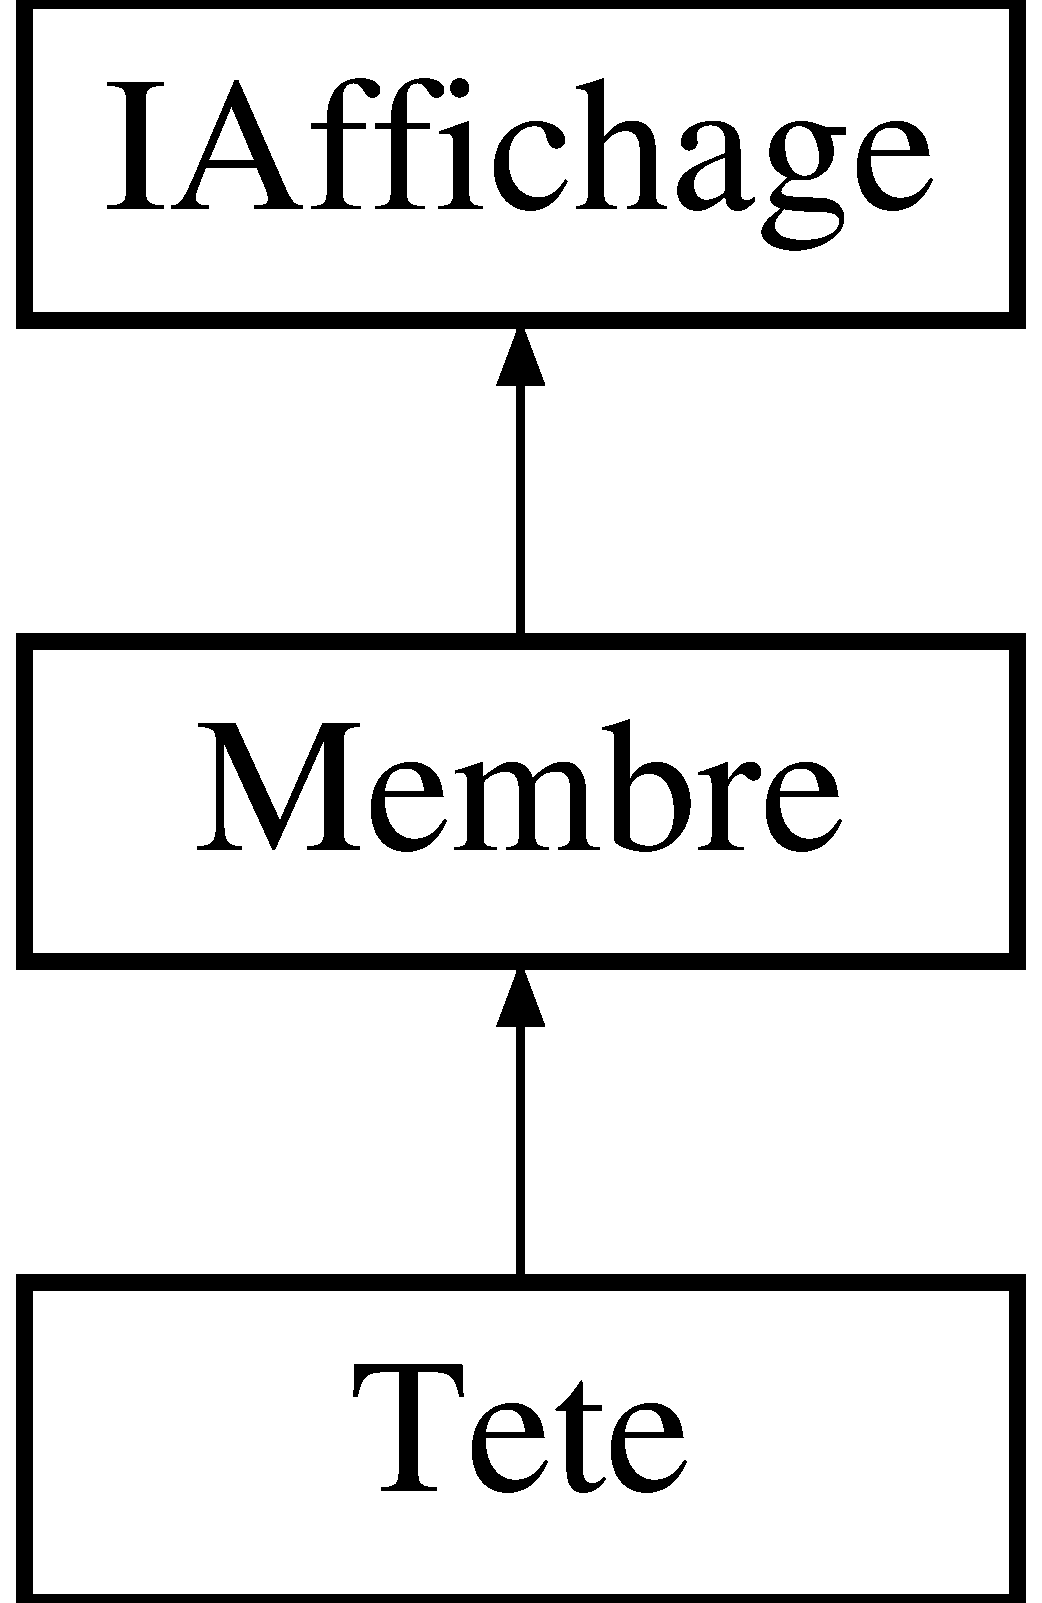
\includegraphics[height=3.000000cm]{class_tete}
\end{center}
\end{figure}
\subsection*{\-Public \-Member \-Functions}
\begin{DoxyCompactItemize}
\item 
\hyperlink{class_tete_a0e1d458209193725c9f615a9ca5b13f1}{\-Tete} ()
\item 
int \hyperlink{class_tete_a78683bd6baef917ed2db10f1a703b0ac}{get\-Id} ()
\item 
void \hyperlink{class_tete_adf73f2de90a86656810db42e96033858}{set\-Id} (int id)
\item 
int \hyperlink{class_tete_aa2c9934f7442d9a5e8cb2fc5c050e554}{get\-P\-D\-V} ()
\item 
void \hyperlink{class_tete_a07df0ae5bc33c6c6c216541046e3995a}{set\-P\-D\-V} (int p)
\item 
string \hyperlink{class_tete_afb6abc9aae3bd726acbe7f725d6ffa96}{get\-Libelle} ()
\item 
void \hyperlink{class_tete_a644eff8bb48835a4e82e848411e30ae8}{set\-Libelle} (string l)
\item 
\hyperlink{class_equipement}{\-Equipement} \hyperlink{class_tete_ae0e3b91eca717e2e5479f72feaef5b90}{get\-Equip} ()
\item 
\hyperlink{class_equipement}{\-Equipement} \hyperlink{class_tete_a126334fb3e157995becf73c2ba3ff10c}{set\-Equip} (\hyperlink{class_equipement}{\-Equipement} e)
\end{DoxyCompactItemize}


\subsection{\-Detailed \-Description}
\-Classe \hyperlink{class_tete}{\-Tete}, hérite de \hyperlink{class_membre}{\-Membre} 

\subsection{\-Constructor \& \-Destructor \-Documentation}
\hypertarget{class_tete_a0e1d458209193725c9f615a9ca5b13f1}{\index{\-Tete@{\-Tete}!\-Tete@{\-Tete}}
\index{\-Tete@{\-Tete}!Tete@{\-Tete}}
\subsubsection[{\-Tete}]{\setlength{\rightskip}{0pt plus 5cm}{\bf \-Tete\-::\-Tete} (
\begin{DoxyParamCaption}
{}
\end{DoxyParamCaption}
)\hspace{0.3cm}{\ttfamily  \mbox{[}inline\mbox{]}}}}\label{class_tete_a0e1d458209193725c9f615a9ca5b13f1}
\-Constructeur explicite initialisant les variables de la tête 

\subsection{\-Member \-Function \-Documentation}
\hypertarget{class_tete_ae0e3b91eca717e2e5479f72feaef5b90}{\index{\-Tete@{\-Tete}!get\-Equip@{get\-Equip}}
\index{get\-Equip@{get\-Equip}!Tete@{\-Tete}}
\subsubsection[{get\-Equip}]{\setlength{\rightskip}{0pt plus 5cm}{\bf \-Equipement} {\bf \-Tete\-::get\-Equip} (
\begin{DoxyParamCaption}
{}
\end{DoxyParamCaption}
)\hspace{0.3cm}{\ttfamily  \mbox{[}inline\mbox{]}}}}\label{class_tete_ae0e3b91eca717e2e5479f72feaef5b90}
\-Accesseur à l'\hyperlink{class_equipement}{\-Equipement} équipé à la tête 

\-Reimplemented from \hyperlink{class_membre_a8b57b95b91806ebf6171624ac0a051cb}{\-Membre}.

\hypertarget{class_tete_a78683bd6baef917ed2db10f1a703b0ac}{\index{\-Tete@{\-Tete}!get\-Id@{get\-Id}}
\index{get\-Id@{get\-Id}!Tete@{\-Tete}}
\subsubsection[{get\-Id}]{\setlength{\rightskip}{0pt plus 5cm}int {\bf \-Tete\-::get\-Id} (
\begin{DoxyParamCaption}
{}
\end{DoxyParamCaption}
)\hspace{0.3cm}{\ttfamily  \mbox{[}inline\mbox{]}}}}\label{class_tete_a78683bd6baef917ed2db10f1a703b0ac}
\-Accesseur à l'identifiant de la tête 

\-Reimplemented from \hyperlink{class_membre_aa4ba3c5babf132246cc84907c37e3738}{\-Membre}.

\hypertarget{class_tete_afb6abc9aae3bd726acbe7f725d6ffa96}{\index{\-Tete@{\-Tete}!get\-Libelle@{get\-Libelle}}
\index{get\-Libelle@{get\-Libelle}!Tete@{\-Tete}}
\subsubsection[{get\-Libelle}]{\setlength{\rightskip}{0pt plus 5cm}string {\bf \-Tete\-::get\-Libelle} (
\begin{DoxyParamCaption}
{}
\end{DoxyParamCaption}
)\hspace{0.3cm}{\ttfamily  \mbox{[}inline\mbox{]}}}}\label{class_tete_afb6abc9aae3bd726acbe7f725d6ffa96}
\-Accesseur au libellé du membre 

\-Reimplemented from \hyperlink{class_membre_a6ef6931754fe7ce7e8101bf27bc3ef6a}{\-Membre}.

\hypertarget{class_tete_aa2c9934f7442d9a5e8cb2fc5c050e554}{\index{\-Tete@{\-Tete}!get\-P\-D\-V@{get\-P\-D\-V}}
\index{get\-P\-D\-V@{get\-P\-D\-V}!Tete@{\-Tete}}
\subsubsection[{get\-P\-D\-V}]{\setlength{\rightskip}{0pt plus 5cm}int {\bf \-Tete\-::get\-P\-D\-V} (
\begin{DoxyParamCaption}
{}
\end{DoxyParamCaption}
)\hspace{0.3cm}{\ttfamily  \mbox{[}inline\mbox{]}}}}\label{class_tete_aa2c9934f7442d9a5e8cb2fc5c050e554}
\-Accesseur au nombre de points de vie de la tête 

\-Reimplemented from \hyperlink{class_membre_a35ddd831b2ca01dd13be213470f2aa65}{\-Membre}.

\hypertarget{class_tete_a126334fb3e157995becf73c2ba3ff10c}{\index{\-Tete@{\-Tete}!set\-Equip@{set\-Equip}}
\index{set\-Equip@{set\-Equip}!Tete@{\-Tete}}
\subsubsection[{set\-Equip}]{\setlength{\rightskip}{0pt plus 5cm}{\bf \-Equipement} {\bf \-Tete\-::set\-Equip} (
\begin{DoxyParamCaption}
\item[{{\bf \-Equipement}}]{e}
\end{DoxyParamCaption}
)\hspace{0.3cm}{\ttfamily  \mbox{[}inline\mbox{]}}}}\label{class_tete_a126334fb3e157995becf73c2ba3ff10c}
\-Mutateur de l'\hyperlink{class_equipement}{\-Equipement} équipé à la tête 

\-Reimplemented from \hyperlink{class_membre_ab2f78da0480458242168b57cf33e3f7c}{\-Membre}.

\hypertarget{class_tete_adf73f2de90a86656810db42e96033858}{\index{\-Tete@{\-Tete}!set\-Id@{set\-Id}}
\index{set\-Id@{set\-Id}!Tete@{\-Tete}}
\subsubsection[{set\-Id}]{\setlength{\rightskip}{0pt plus 5cm}void {\bf \-Tete\-::set\-Id} (
\begin{DoxyParamCaption}
\item[{int}]{id}
\end{DoxyParamCaption}
)\hspace{0.3cm}{\ttfamily  \mbox{[}inline\mbox{]}}}}\label{class_tete_adf73f2de90a86656810db42e96033858}
\-Mutateur de l'identifiant de la tête 

\-Reimplemented from \hyperlink{class_membre_a4b87bebc56e82f08d4ebdf8bcf773c11}{\-Membre}.

\hypertarget{class_tete_a644eff8bb48835a4e82e848411e30ae8}{\index{\-Tete@{\-Tete}!set\-Libelle@{set\-Libelle}}
\index{set\-Libelle@{set\-Libelle}!Tete@{\-Tete}}
\subsubsection[{set\-Libelle}]{\setlength{\rightskip}{0pt plus 5cm}void {\bf \-Tete\-::set\-Libelle} (
\begin{DoxyParamCaption}
\item[{string}]{l}
\end{DoxyParamCaption}
)\hspace{0.3cm}{\ttfamily  \mbox{[}inline\mbox{]}}}}\label{class_tete_a644eff8bb48835a4e82e848411e30ae8}
\-Mutateur du libellé du membre 

\-Reimplemented from \hyperlink{class_membre_aaffef4990f332871cd1dd9b3fc03a078}{\-Membre}.

\hypertarget{class_tete_a07df0ae5bc33c6c6c216541046e3995a}{\index{\-Tete@{\-Tete}!set\-P\-D\-V@{set\-P\-D\-V}}
\index{set\-P\-D\-V@{set\-P\-D\-V}!Tete@{\-Tete}}
\subsubsection[{set\-P\-D\-V}]{\setlength{\rightskip}{0pt plus 5cm}void {\bf \-Tete\-::set\-P\-D\-V} (
\begin{DoxyParamCaption}
\item[{int}]{p}
\end{DoxyParamCaption}
)\hspace{0.3cm}{\ttfamily  \mbox{[}inline\mbox{]}}}}\label{class_tete_a07df0ae5bc33c6c6c216541046e3995a}
\-Mutateur du nombre de points de vie de la tête 

\-Reimplemented from \hyperlink{class_membre_a6b45657cd705c02a6ab5a338d1204f3e}{\-Membre}.



\-The documentation for this class was generated from the following file\-:\begin{DoxyCompactItemize}
\item 
\-Projet\-P\-O\-O-\/master/\-Tete.\-cpp\end{DoxyCompactItemize}

\hypertarget{class_thraex}{\section{\-Thraex \-Class \-Reference}
\label{class_thraex}\index{\-Thraex@{\-Thraex}}
}
\-Inheritance diagram for \-Thraex\-:\begin{figure}[H]
\begin{center}
\leavevmode
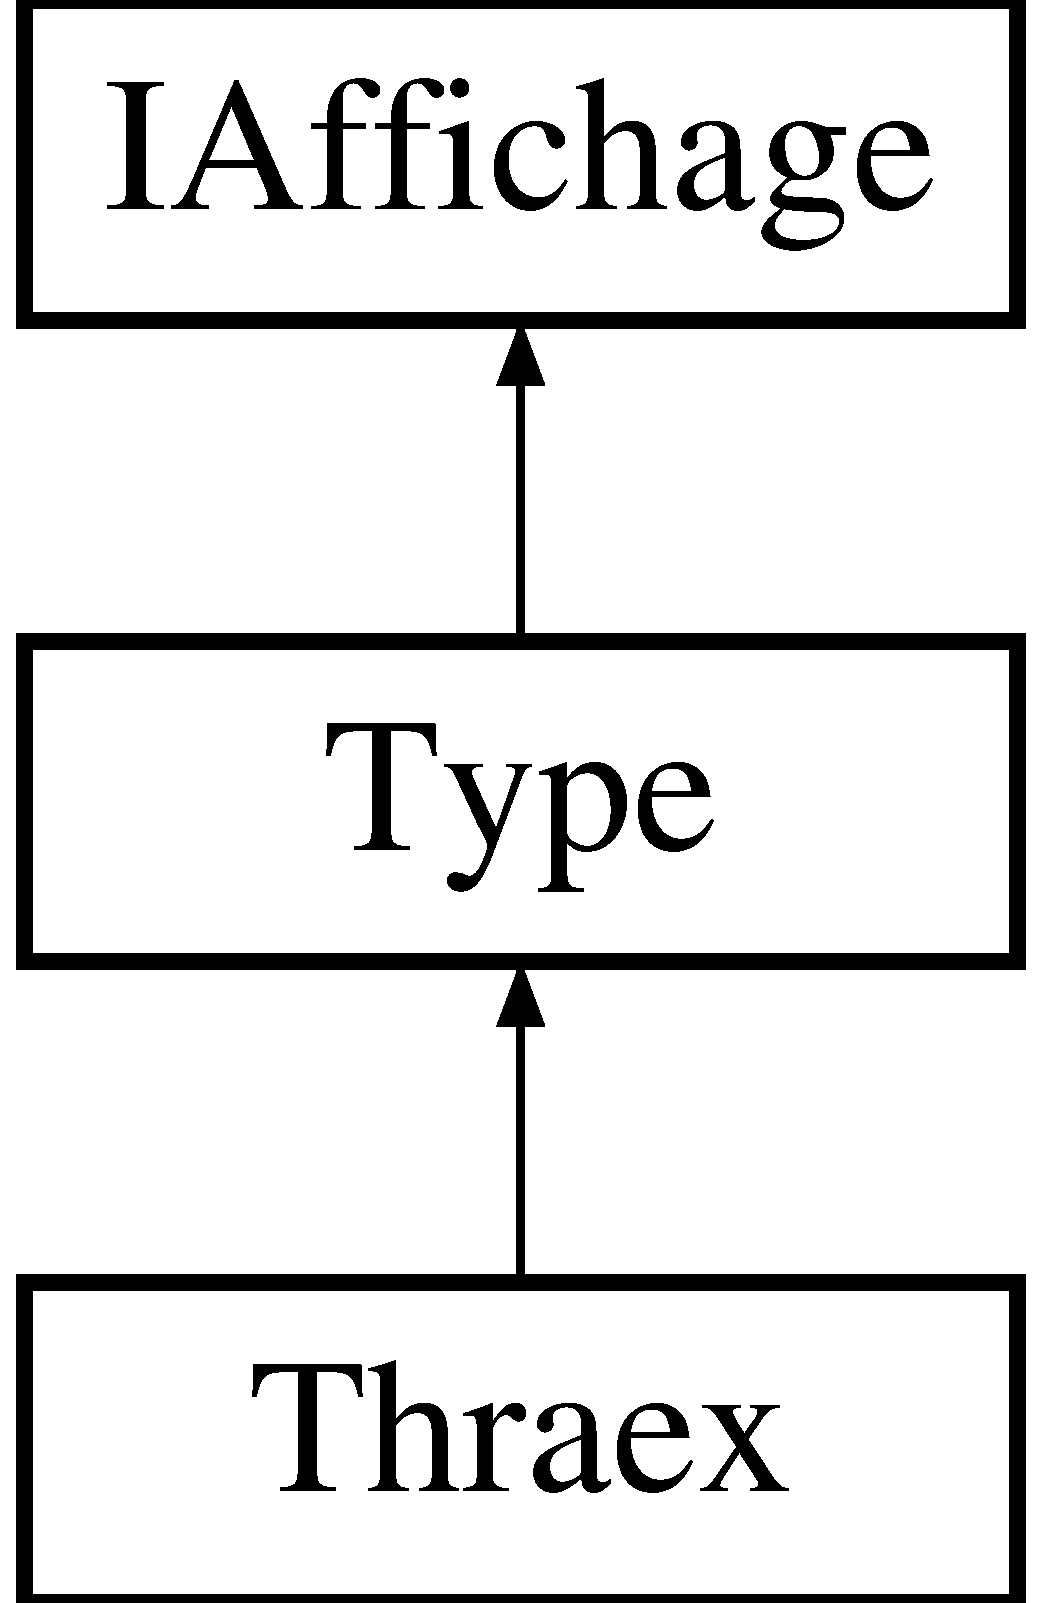
\includegraphics[height=3.000000cm]{class_thraex}
\end{center}
\end{figure}
\subsection*{\-Public \-Member \-Functions}
\begin{DoxyCompactItemize}
\item 
\hyperlink{class_thraex_a90072ae3cc86b80cf2eda276772a87ee}{\-Thraex} ()
\item 
int \hyperlink{class_thraex_a5d94cdc56d14414232cac77159c9ab1b}{get\-Id} ()
\item 
void \hyperlink{class_thraex_a6ac63b6366fe06fb6c1220366a429688}{set\-Id} (int id)
\item 
string \hyperlink{class_thraex_a65ee8774373a984717ba1ed4e9f4bd41}{get\-Libelle} ()
\item 
void \hyperlink{class_thraex_a17fc7a95847ecc16da4ca3a4b5edc574}{set\-Libelle} (string l)
\end{DoxyCompactItemize}


\subsection{\-Detailed \-Description}
\-Classe \hyperlink{class_thraex}{\-Thraex}, hérite de \hyperlink{class_type}{\-Type} 

\subsection{\-Constructor \& \-Destructor \-Documentation}
\hypertarget{class_thraex_a90072ae3cc86b80cf2eda276772a87ee}{\index{\-Thraex@{\-Thraex}!\-Thraex@{\-Thraex}}
\index{\-Thraex@{\-Thraex}!Thraex@{\-Thraex}}
\subsubsection[{\-Thraex}]{\setlength{\rightskip}{0pt plus 5cm}{\bf \-Thraex\-::\-Thraex} (
\begin{DoxyParamCaption}
{}
\end{DoxyParamCaption}
)\hspace{0.3cm}{\ttfamily  \mbox{[}inline\mbox{]}}}}\label{class_thraex_a90072ae3cc86b80cf2eda276772a87ee}
\-Constructeur explicite initialisant les variables du type 

\subsection{\-Member \-Function \-Documentation}
\hypertarget{class_thraex_a5d94cdc56d14414232cac77159c9ab1b}{\index{\-Thraex@{\-Thraex}!get\-Id@{get\-Id}}
\index{get\-Id@{get\-Id}!Thraex@{\-Thraex}}
\subsubsection[{get\-Id}]{\setlength{\rightskip}{0pt plus 5cm}int {\bf \-Thraex\-::get\-Id} (
\begin{DoxyParamCaption}
{}
\end{DoxyParamCaption}
)\hspace{0.3cm}{\ttfamily  \mbox{[}inline\mbox{]}}}}\label{class_thraex_a5d94cdc56d14414232cac77159c9ab1b}
\-Accesseur à l'identifiant du type 

\-Reimplemented from \hyperlink{class_type_aba890fe7677f58f7135ec0cfe1b7c926}{\-Type}.

\hypertarget{class_thraex_a65ee8774373a984717ba1ed4e9f4bd41}{\index{\-Thraex@{\-Thraex}!get\-Libelle@{get\-Libelle}}
\index{get\-Libelle@{get\-Libelle}!Thraex@{\-Thraex}}
\subsubsection[{get\-Libelle}]{\setlength{\rightskip}{0pt plus 5cm}string {\bf \-Thraex\-::get\-Libelle} (
\begin{DoxyParamCaption}
{}
\end{DoxyParamCaption}
)\hspace{0.3cm}{\ttfamily  \mbox{[}inline\mbox{]}}}}\label{class_thraex_a65ee8774373a984717ba1ed4e9f4bd41}
\-Accesseur au libellé du type 

\-Reimplemented from \hyperlink{class_type_a38a529eb6a80a3d3cb801996cc9f41f0}{\-Type}.

\hypertarget{class_thraex_a6ac63b6366fe06fb6c1220366a429688}{\index{\-Thraex@{\-Thraex}!set\-Id@{set\-Id}}
\index{set\-Id@{set\-Id}!Thraex@{\-Thraex}}
\subsubsection[{set\-Id}]{\setlength{\rightskip}{0pt plus 5cm}void {\bf \-Thraex\-::set\-Id} (
\begin{DoxyParamCaption}
\item[{int}]{id}
\end{DoxyParamCaption}
)\hspace{0.3cm}{\ttfamily  \mbox{[}inline\mbox{]}}}}\label{class_thraex_a6ac63b6366fe06fb6c1220366a429688}
\-Mutateur de l'identifiant du type 

\-Reimplemented from \hyperlink{class_type_ab9b8158dca9be6184557382ec98ec4f7}{\-Type}.

\hypertarget{class_thraex_a17fc7a95847ecc16da4ca3a4b5edc574}{\index{\-Thraex@{\-Thraex}!set\-Libelle@{set\-Libelle}}
\index{set\-Libelle@{set\-Libelle}!Thraex@{\-Thraex}}
\subsubsection[{set\-Libelle}]{\setlength{\rightskip}{0pt plus 5cm}void {\bf \-Thraex\-::set\-Libelle} (
\begin{DoxyParamCaption}
\item[{string}]{l}
\end{DoxyParamCaption}
)\hspace{0.3cm}{\ttfamily  \mbox{[}inline\mbox{]}}}}\label{class_thraex_a17fc7a95847ecc16da4ca3a4b5edc574}
\-Mutateur du libellé du type 

\-Reimplemented from \hyperlink{class_type_af475df921624fe329aaa6b19bd1ed2e1}{\-Type}.



\-The documentation for this class was generated from the following file\-:\begin{DoxyCompactItemize}
\item 
\-Projet\-P\-O\-O-\/master/\-Thraex.\-cpp\end{DoxyCompactItemize}

\hypertarget{class_torse}{\section{\-Torse \-Class \-Reference}
\label{class_torse}\index{\-Torse@{\-Torse}}
}
\-Inheritance diagram for \-Torse\-:\begin{figure}[H]
\begin{center}
\leavevmode
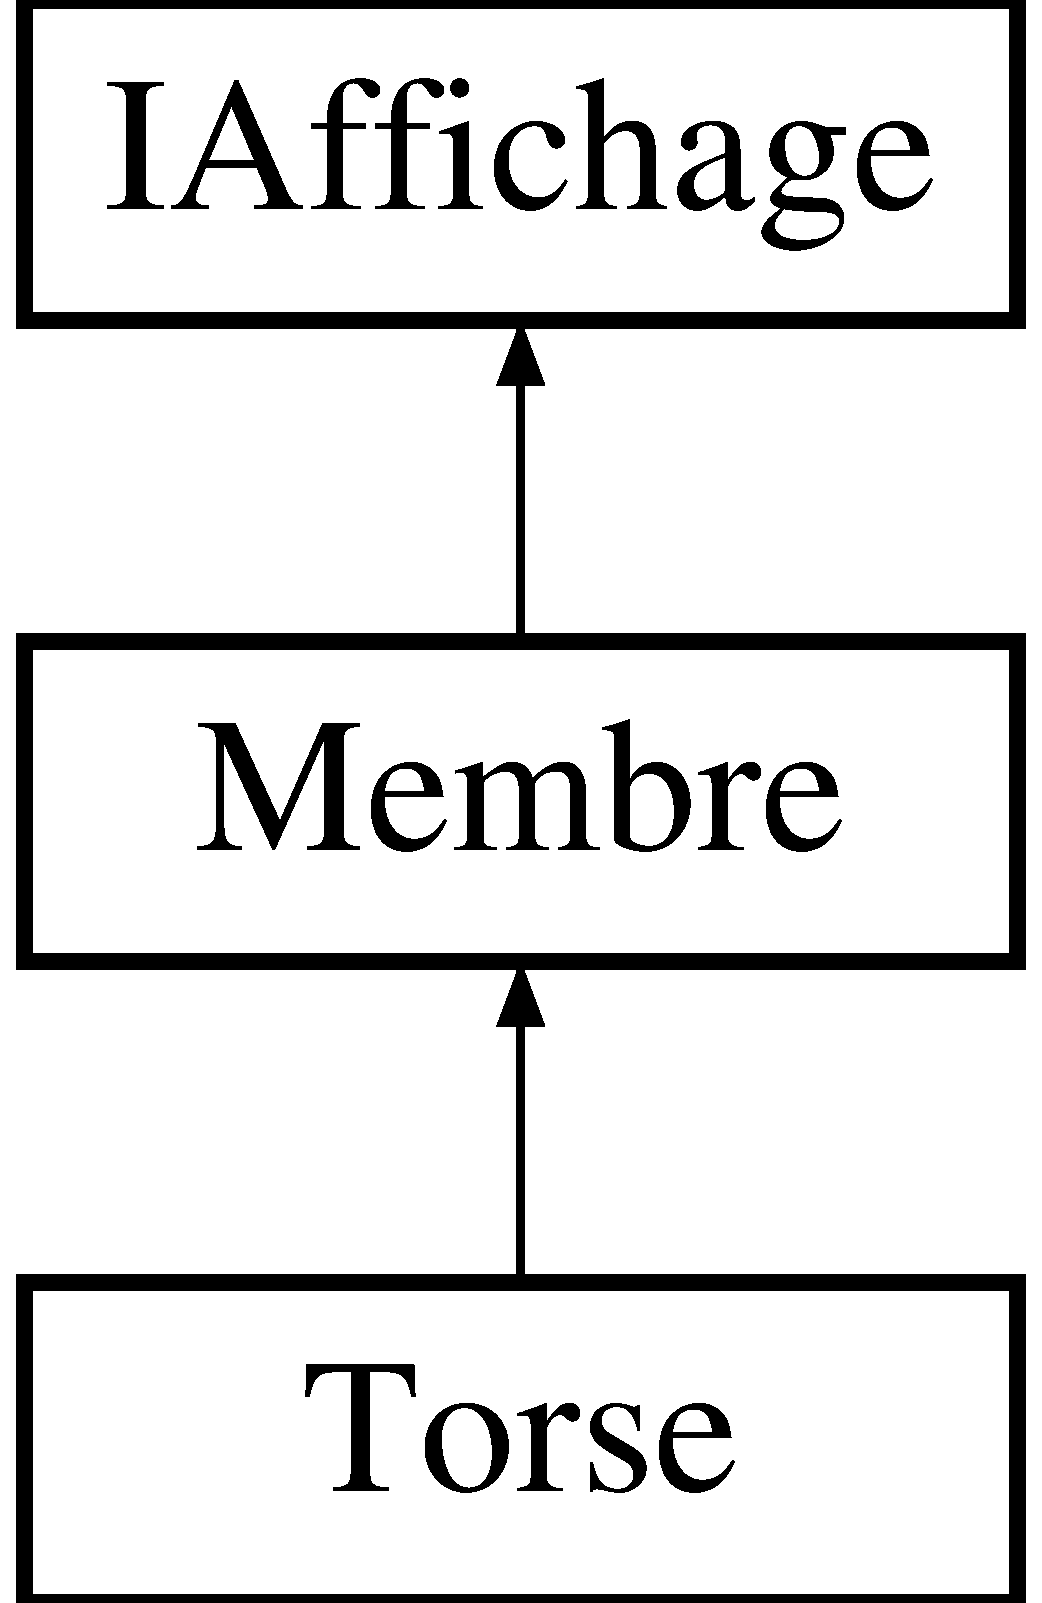
\includegraphics[height=3.000000cm]{class_torse}
\end{center}
\end{figure}
\subsection*{\-Public \-Member \-Functions}
\begin{DoxyCompactItemize}
\item 
\hyperlink{class_torse_a5bfcd88fc96057dd794cbae945d0b541}{\-Torse} ()
\item 
int \hyperlink{class_torse_a58614d9c4ce5021515e9a09d68e3366e}{get\-Id} ()
\item 
void \hyperlink{class_torse_a797b1977bbc9dd5ab6bb5b6731e3081f}{set\-Id} (int id)
\item 
int \hyperlink{class_torse_a2f13314c8454f1be93a17ecd3be02408}{get\-P\-D\-V} ()
\item 
void \hyperlink{class_torse_a88aeb0ac624296d654a245522e9a7a4c}{set\-P\-D\-V} (int p)
\item 
string \hyperlink{class_torse_a4e2fefc2b6e0486d26b33edcd50d0fb4}{get\-Libelle} ()
\item 
void \hyperlink{class_torse_a89ac35e98847c1f39f8bdb840efddd75}{set\-Libelle} (string l)
\item 
\hyperlink{class_equipement}{\-Equipement} \hyperlink{class_torse_aef7412e7ca619d0855aa890d84b4a609}{get\-Equip} ()
\item 
\hyperlink{class_equipement}{\-Equipement} \hyperlink{class_torse_a59c9a4895878649516f5f0622cbce083}{set\-Equip} (\hyperlink{class_equipement}{\-Equipement} e)
\end{DoxyCompactItemize}


\subsection{\-Detailed \-Description}
\-Classe \hyperlink{class_torse}{\-Torse}, hérite de \hyperlink{class_membre}{\-Membre} 

\subsection{\-Constructor \& \-Destructor \-Documentation}
\hypertarget{class_torse_a5bfcd88fc96057dd794cbae945d0b541}{\index{\-Torse@{\-Torse}!\-Torse@{\-Torse}}
\index{\-Torse@{\-Torse}!Torse@{\-Torse}}
\subsubsection[{\-Torse}]{\setlength{\rightskip}{0pt plus 5cm}{\bf \-Torse\-::\-Torse} (
\begin{DoxyParamCaption}
{}
\end{DoxyParamCaption}
)\hspace{0.3cm}{\ttfamily  \mbox{[}inline\mbox{]}}}}\label{class_torse_a5bfcd88fc96057dd794cbae945d0b541}
\-Constructeur explicite initialisant les variables du torse 

\subsection{\-Member \-Function \-Documentation}
\hypertarget{class_torse_aef7412e7ca619d0855aa890d84b4a609}{\index{\-Torse@{\-Torse}!get\-Equip@{get\-Equip}}
\index{get\-Equip@{get\-Equip}!Torse@{\-Torse}}
\subsubsection[{get\-Equip}]{\setlength{\rightskip}{0pt plus 5cm}{\bf \-Equipement} {\bf \-Torse\-::get\-Equip} (
\begin{DoxyParamCaption}
{}
\end{DoxyParamCaption}
)\hspace{0.3cm}{\ttfamily  \mbox{[}inline\mbox{]}}}}\label{class_torse_aef7412e7ca619d0855aa890d84b4a609}
\-Accesseur à l'\hyperlink{class_equipement}{\-Equipement} équipé au torse 

\-Reimplemented from \hyperlink{class_membre_a8b57b95b91806ebf6171624ac0a051cb}{\-Membre}.

\hypertarget{class_torse_a58614d9c4ce5021515e9a09d68e3366e}{\index{\-Torse@{\-Torse}!get\-Id@{get\-Id}}
\index{get\-Id@{get\-Id}!Torse@{\-Torse}}
\subsubsection[{get\-Id}]{\setlength{\rightskip}{0pt plus 5cm}int {\bf \-Torse\-::get\-Id} (
\begin{DoxyParamCaption}
{}
\end{DoxyParamCaption}
)\hspace{0.3cm}{\ttfamily  \mbox{[}inline\mbox{]}}}}\label{class_torse_a58614d9c4ce5021515e9a09d68e3366e}
\-Accesseur à l'identifiant du torse 

\-Reimplemented from \hyperlink{class_membre_aa4ba3c5babf132246cc84907c37e3738}{\-Membre}.

\hypertarget{class_torse_a4e2fefc2b6e0486d26b33edcd50d0fb4}{\index{\-Torse@{\-Torse}!get\-Libelle@{get\-Libelle}}
\index{get\-Libelle@{get\-Libelle}!Torse@{\-Torse}}
\subsubsection[{get\-Libelle}]{\setlength{\rightskip}{0pt plus 5cm}string {\bf \-Torse\-::get\-Libelle} (
\begin{DoxyParamCaption}
{}
\end{DoxyParamCaption}
)\hspace{0.3cm}{\ttfamily  \mbox{[}inline\mbox{]}}}}\label{class_torse_a4e2fefc2b6e0486d26b33edcd50d0fb4}
\-Accesseur au libellé du membre 

\-Reimplemented from \hyperlink{class_membre_a6ef6931754fe7ce7e8101bf27bc3ef6a}{\-Membre}.

\hypertarget{class_torse_a2f13314c8454f1be93a17ecd3be02408}{\index{\-Torse@{\-Torse}!get\-P\-D\-V@{get\-P\-D\-V}}
\index{get\-P\-D\-V@{get\-P\-D\-V}!Torse@{\-Torse}}
\subsubsection[{get\-P\-D\-V}]{\setlength{\rightskip}{0pt plus 5cm}int {\bf \-Torse\-::get\-P\-D\-V} (
\begin{DoxyParamCaption}
{}
\end{DoxyParamCaption}
)\hspace{0.3cm}{\ttfamily  \mbox{[}inline\mbox{]}}}}\label{class_torse_a2f13314c8454f1be93a17ecd3be02408}
\-Accesseur au nombre de points de vie du torse 

\-Reimplemented from \hyperlink{class_membre_a35ddd831b2ca01dd13be213470f2aa65}{\-Membre}.

\hypertarget{class_torse_a59c9a4895878649516f5f0622cbce083}{\index{\-Torse@{\-Torse}!set\-Equip@{set\-Equip}}
\index{set\-Equip@{set\-Equip}!Torse@{\-Torse}}
\subsubsection[{set\-Equip}]{\setlength{\rightskip}{0pt plus 5cm}{\bf \-Equipement} {\bf \-Torse\-::set\-Equip} (
\begin{DoxyParamCaption}
\item[{{\bf \-Equipement}}]{e}
\end{DoxyParamCaption}
)\hspace{0.3cm}{\ttfamily  \mbox{[}inline\mbox{]}}}}\label{class_torse_a59c9a4895878649516f5f0622cbce083}
\-Mutateur de l'\hyperlink{class_equipement}{\-Equipement} équipé au torse 

\-Reimplemented from \hyperlink{class_membre_ab2f78da0480458242168b57cf33e3f7c}{\-Membre}.

\hypertarget{class_torse_a797b1977bbc9dd5ab6bb5b6731e3081f}{\index{\-Torse@{\-Torse}!set\-Id@{set\-Id}}
\index{set\-Id@{set\-Id}!Torse@{\-Torse}}
\subsubsection[{set\-Id}]{\setlength{\rightskip}{0pt plus 5cm}void {\bf \-Torse\-::set\-Id} (
\begin{DoxyParamCaption}
\item[{int}]{id}
\end{DoxyParamCaption}
)\hspace{0.3cm}{\ttfamily  \mbox{[}inline\mbox{]}}}}\label{class_torse_a797b1977bbc9dd5ab6bb5b6731e3081f}
\-Mutateur de l'identifiant du torse 

\-Reimplemented from \hyperlink{class_membre_a4b87bebc56e82f08d4ebdf8bcf773c11}{\-Membre}.

\hypertarget{class_torse_a89ac35e98847c1f39f8bdb840efddd75}{\index{\-Torse@{\-Torse}!set\-Libelle@{set\-Libelle}}
\index{set\-Libelle@{set\-Libelle}!Torse@{\-Torse}}
\subsubsection[{set\-Libelle}]{\setlength{\rightskip}{0pt plus 5cm}void {\bf \-Torse\-::set\-Libelle} (
\begin{DoxyParamCaption}
\item[{string}]{l}
\end{DoxyParamCaption}
)\hspace{0.3cm}{\ttfamily  \mbox{[}inline\mbox{]}}}}\label{class_torse_a89ac35e98847c1f39f8bdb840efddd75}
\-Mutateur du libellé du membre 

\-Reimplemented from \hyperlink{class_membre_aaffef4990f332871cd1dd9b3fc03a078}{\-Membre}.

\hypertarget{class_torse_a88aeb0ac624296d654a245522e9a7a4c}{\index{\-Torse@{\-Torse}!set\-P\-D\-V@{set\-P\-D\-V}}
\index{set\-P\-D\-V@{set\-P\-D\-V}!Torse@{\-Torse}}
\subsubsection[{set\-P\-D\-V}]{\setlength{\rightskip}{0pt plus 5cm}void {\bf \-Torse\-::set\-P\-D\-V} (
\begin{DoxyParamCaption}
\item[{int}]{p}
\end{DoxyParamCaption}
)\hspace{0.3cm}{\ttfamily  \mbox{[}inline\mbox{]}}}}\label{class_torse_a88aeb0ac624296d654a245522e9a7a4c}
\-Mutateur du nombre de points de vie du torse 

\-Reimplemented from \hyperlink{class_membre_a6b45657cd705c02a6ab5a338d1204f3e}{\-Membre}.



\-The documentation for this class was generated from the following file\-:\begin{DoxyCompactItemize}
\item 
\-Projet\-P\-O\-O-\/master/\-Torse.\-cpp\end{DoxyCompactItemize}

\hypertarget{class_trident}{\section{\-Trident \-Class \-Reference}
\label{class_trident}\index{\-Trident@{\-Trident}}
}
\-Inheritance diagram for \-Trident\-:\begin{figure}[H]
\begin{center}
\leavevmode
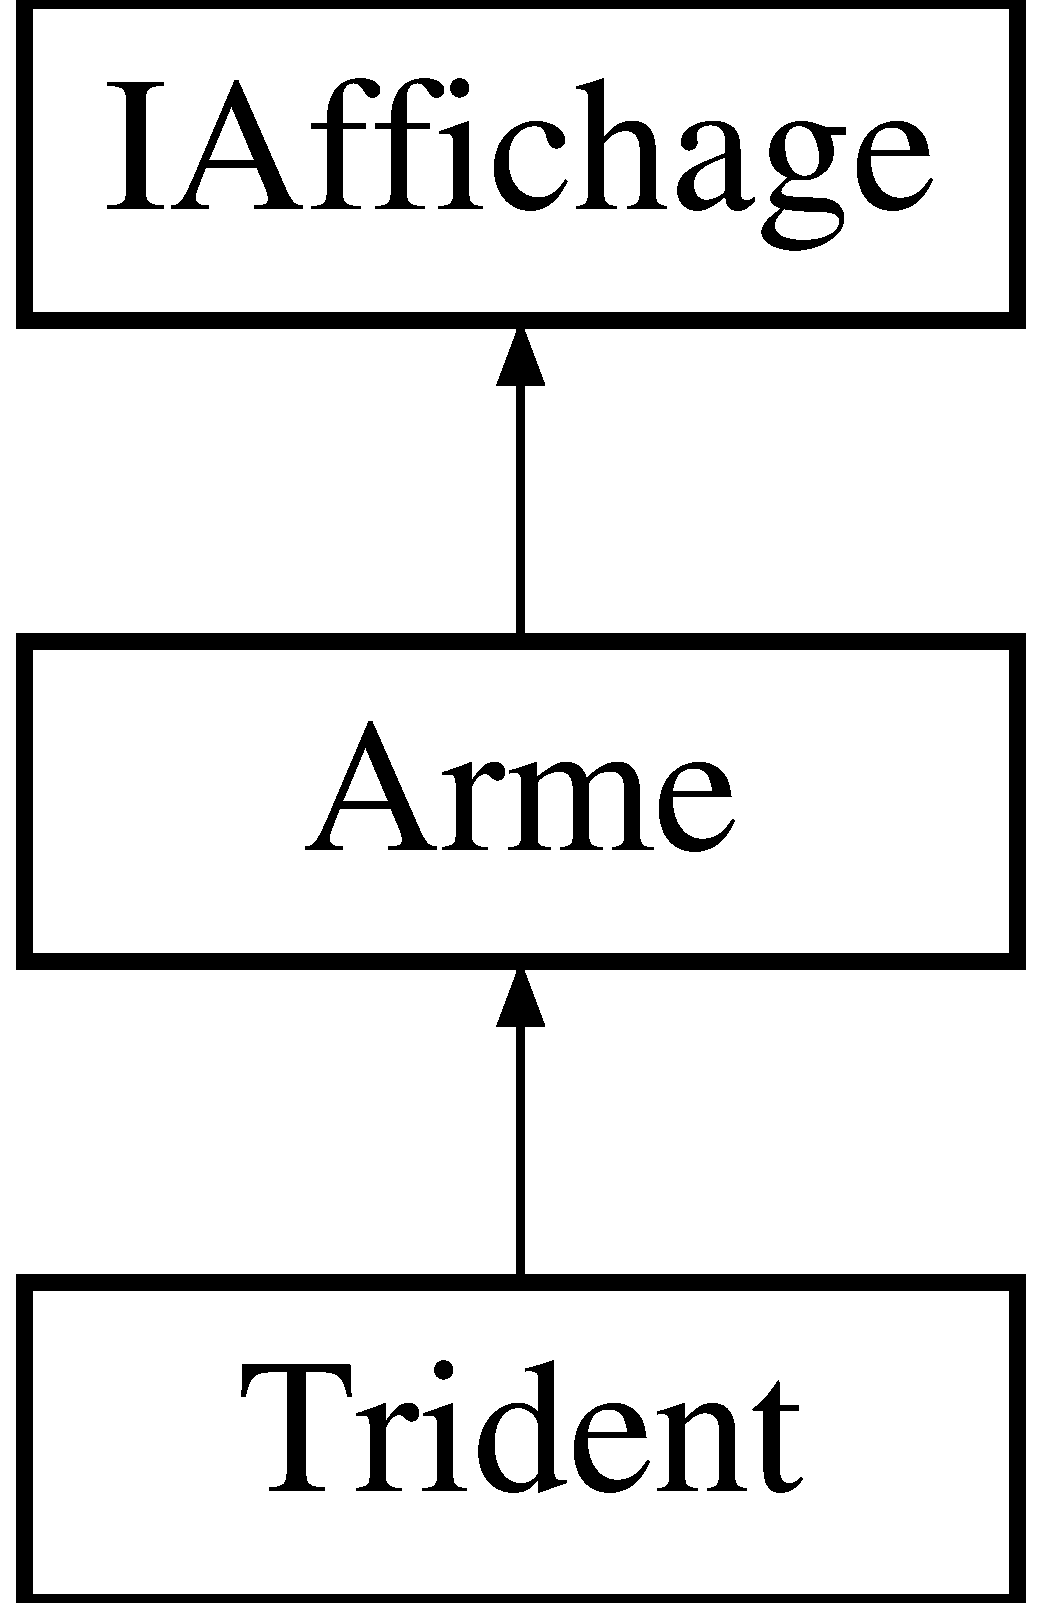
\includegraphics[height=3.000000cm]{class_trident}
\end{center}
\end{figure}
\subsection*{\-Public \-Member \-Functions}
\begin{DoxyCompactItemize}
\item 
\hyperlink{class_trident_a0b3745e319e2826941a5106f9b5a7536}{\-Trident} ()
\item 
int \hyperlink{class_trident_af6ffe8225c67ee4404cd0a571453a113}{get\-Id} ()
\item 
void \hyperlink{class_trident_a3e64bc6cde8ae2e03875c7d256282de8}{set\-Id} (int id)
\item 
string \hyperlink{class_trident_a5a674900b64b6fb658828f99cbc222a5}{get\-Libelle} ()
\item 
void \hyperlink{class_trident_ac9bc02a8c00777defffcc50cd8f42619}{set\-Libelle} (string l)
\item 
int \hyperlink{class_trident_aa253e2ac8326becccd89b8066273a2e1}{get\-Val\-Deg} ()
\item 
void \hyperlink{class_trident_aec340f9c7063794b56845e86dea3da09}{set\-Val\-Deg} (int v)
\end{DoxyCompactItemize}


\subsection{\-Detailed \-Description}
\-Classe \hyperlink{class_trident}{\-Trident}, hérite d'\hyperlink{class_arme}{\-Arme} 

\subsection{\-Constructor \& \-Destructor \-Documentation}
\hypertarget{class_trident_a0b3745e319e2826941a5106f9b5a7536}{\index{\-Trident@{\-Trident}!\-Trident@{\-Trident}}
\index{\-Trident@{\-Trident}!Trident@{\-Trident}}
\subsubsection[{\-Trident}]{\setlength{\rightskip}{0pt plus 5cm}{\bf \-Trident\-::\-Trident} (
\begin{DoxyParamCaption}
{}
\end{DoxyParamCaption}
)\hspace{0.3cm}{\ttfamily  \mbox{[}inline\mbox{]}}}}\label{class_trident_a0b3745e319e2826941a5106f9b5a7536}
\-Constructeur explicite initialisant les variables du trident 

\subsection{\-Member \-Function \-Documentation}
\hypertarget{class_trident_af6ffe8225c67ee4404cd0a571453a113}{\index{\-Trident@{\-Trident}!get\-Id@{get\-Id}}
\index{get\-Id@{get\-Id}!Trident@{\-Trident}}
\subsubsection[{get\-Id}]{\setlength{\rightskip}{0pt plus 5cm}int {\bf \-Trident\-::get\-Id} (
\begin{DoxyParamCaption}
{}
\end{DoxyParamCaption}
)\hspace{0.3cm}{\ttfamily  \mbox{[}inline\mbox{]}}}}\label{class_trident_af6ffe8225c67ee4404cd0a571453a113}
\-Accesseur à l'identifiant du trident 

\-Reimplemented from \hyperlink{class_arme_a6c957484697d9ad38ab1ed4361f3b8f4}{\-Arme}.

\hypertarget{class_trident_a5a674900b64b6fb658828f99cbc222a5}{\index{\-Trident@{\-Trident}!get\-Libelle@{get\-Libelle}}
\index{get\-Libelle@{get\-Libelle}!Trident@{\-Trident}}
\subsubsection[{get\-Libelle}]{\setlength{\rightskip}{0pt plus 5cm}string {\bf \-Trident\-::get\-Libelle} (
\begin{DoxyParamCaption}
{}
\end{DoxyParamCaption}
)\hspace{0.3cm}{\ttfamily  \mbox{[}inline\mbox{]}}}}\label{class_trident_a5a674900b64b6fb658828f99cbc222a5}
\-Accesseur au libellé de l'arme 

\-Reimplemented from \hyperlink{class_arme_a5e43d33d0e14da19fb37dc497474135b}{\-Arme}.

\hypertarget{class_trident_aa253e2ac8326becccd89b8066273a2e1}{\index{\-Trident@{\-Trident}!get\-Val\-Deg@{get\-Val\-Deg}}
\index{get\-Val\-Deg@{get\-Val\-Deg}!Trident@{\-Trident}}
\subsubsection[{get\-Val\-Deg}]{\setlength{\rightskip}{0pt plus 5cm}int {\bf \-Trident\-::get\-Val\-Deg} (
\begin{DoxyParamCaption}
{}
\end{DoxyParamCaption}
)\hspace{0.3cm}{\ttfamily  \mbox{[}inline\mbox{]}}}}\label{class_trident_aa253e2ac8326becccd89b8066273a2e1}
\-Accesseur à la valeur de dégâts du trident \hypertarget{class_trident_a3e64bc6cde8ae2e03875c7d256282de8}{\index{\-Trident@{\-Trident}!set\-Id@{set\-Id}}
\index{set\-Id@{set\-Id}!Trident@{\-Trident}}
\subsubsection[{set\-Id}]{\setlength{\rightskip}{0pt plus 5cm}void {\bf \-Trident\-::set\-Id} (
\begin{DoxyParamCaption}
\item[{int}]{id}
\end{DoxyParamCaption}
)\hspace{0.3cm}{\ttfamily  \mbox{[}inline\mbox{]}}}}\label{class_trident_a3e64bc6cde8ae2e03875c7d256282de8}
\-Mutateur de l'identifiant du trident 

\-Reimplemented from \hyperlink{class_arme_a332699f4c7b2dab9e38fccfddba7275b}{\-Arme}.

\hypertarget{class_trident_ac9bc02a8c00777defffcc50cd8f42619}{\index{\-Trident@{\-Trident}!set\-Libelle@{set\-Libelle}}
\index{set\-Libelle@{set\-Libelle}!Trident@{\-Trident}}
\subsubsection[{set\-Libelle}]{\setlength{\rightskip}{0pt plus 5cm}void {\bf \-Trident\-::set\-Libelle} (
\begin{DoxyParamCaption}
\item[{string}]{l}
\end{DoxyParamCaption}
)\hspace{0.3cm}{\ttfamily  \mbox{[}inline\mbox{]}}}}\label{class_trident_ac9bc02a8c00777defffcc50cd8f42619}
\-Mutateur du libellé de l'arme 

\-Reimplemented from \hyperlink{class_arme_ab38eebb032ab6773678ee40f152df6dd}{\-Arme}.

\hypertarget{class_trident_aec340f9c7063794b56845e86dea3da09}{\index{\-Trident@{\-Trident}!set\-Val\-Deg@{set\-Val\-Deg}}
\index{set\-Val\-Deg@{set\-Val\-Deg}!Trident@{\-Trident}}
\subsubsection[{set\-Val\-Deg}]{\setlength{\rightskip}{0pt plus 5cm}void {\bf \-Trident\-::set\-Val\-Deg} (
\begin{DoxyParamCaption}
\item[{int}]{v}
\end{DoxyParamCaption}
)\hspace{0.3cm}{\ttfamily  \mbox{[}inline\mbox{]}}}}\label{class_trident_aec340f9c7063794b56845e86dea3da09}
\-Mutateur de la valeur de dégâts du trident 

\-The documentation for this class was generated from the following file\-:\begin{DoxyCompactItemize}
\item 
\-Projet\-P\-O\-O-\/master/\-Trident.\-cpp\end{DoxyCompactItemize}

\hypertarget{class_type}{\section{\-Type \-Class \-Reference}
\label{class_type}\index{\-Type@{\-Type}}
}
\-Inheritance diagram for \-Type\-:\begin{figure}[H]
\begin{center}
\leavevmode
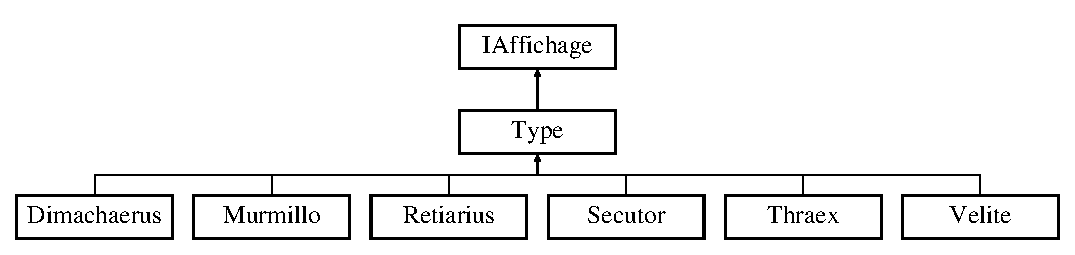
\includegraphics[height=2.978723cm]{class_type}
\end{center}
\end{figure}
\subsection*{\-Public \-Member \-Functions}
\begin{DoxyCompactItemize}
\item 
int \hyperlink{class_type_aba890fe7677f58f7135ec0cfe1b7c926}{get\-Id} ()
\item 
void \hyperlink{class_type_ab9b8158dca9be6184557382ec98ec4f7}{set\-Id} (int id)
\item 
string \hyperlink{class_type_a38a529eb6a80a3d3cb801996cc9f41f0}{get\-Libelle} ()
\item 
void \hyperlink{class_type_af475df921624fe329aaa6b19bd1ed2e1}{set\-Libelle} (string l)
\item 
virtual void \hyperlink{class_type_a793d8cc8a1e9a491803a3e9331e0ddc6}{afficher\-Info} ()
\end{DoxyCompactItemize}


\subsection{\-Detailed \-Description}
\-Classe mère \hyperlink{class_type}{\-Type}, tous les types héritent de celle-\/ci \-Implémente l'interface \hyperlink{class_i_affichage}{\-I\-Affichage} 

\subsection{\-Member \-Function \-Documentation}
\hypertarget{class_type_a793d8cc8a1e9a491803a3e9331e0ddc6}{\index{\-Type@{\-Type}!afficher\-Info@{afficher\-Info}}
\index{afficher\-Info@{afficher\-Info}!Type@{\-Type}}
\subsubsection[{afficher\-Info}]{\setlength{\rightskip}{0pt plus 5cm}virtual void {\bf \-Type\-::afficher\-Info} (
\begin{DoxyParamCaption}
{}
\end{DoxyParamCaption}
)\hspace{0.3cm}{\ttfamily  \mbox{[}inline, virtual\mbox{]}}}}\label{class_type_a793d8cc8a1e9a491803a3e9331e0ddc6}
\-Procédure d'affichage d'informations, redéfinit celle de l'interface \hyperlink{class_i_affichage}{\-I\-Affichage} 

\-Implements \hyperlink{class_i_affichage_a6123c1cb9079f712b48c0b8bf62e14ef}{\-I\-Affichage}.

\hypertarget{class_type_aba890fe7677f58f7135ec0cfe1b7c926}{\index{\-Type@{\-Type}!get\-Id@{get\-Id}}
\index{get\-Id@{get\-Id}!Type@{\-Type}}
\subsubsection[{get\-Id}]{\setlength{\rightskip}{0pt plus 5cm}int {\bf \-Type\-::get\-Id} (
\begin{DoxyParamCaption}
{}
\end{DoxyParamCaption}
)\hspace{0.3cm}{\ttfamily  \mbox{[}inline\mbox{]}}}}\label{class_type_aba890fe7677f58f7135ec0cfe1b7c926}
\-Accesseur à l'identifiant du type 

\-Reimplemented in \hyperlink{class_dimachaerus_a134c3824829dbe4346fcfe149ca8b0bd}{\-Dimachaerus}, \hyperlink{class_murmillo_a90f58f8288899f7ee204b48c4ae99f20}{\-Murmillo}, \hyperlink{class_retiarius_af5b641eab15c0a2c82ecfb3aefd0ec53}{\-Retiarius}, \hyperlink{class_secutor_ad1dddc99e73479adcba390c52f7fd3a9}{\-Secutor}, \hyperlink{class_thraex_a5d94cdc56d14414232cac77159c9ab1b}{\-Thraex}, and \hyperlink{class_velite_a7829a1da010495af34d315084943076e}{\-Velite}.

\hypertarget{class_type_a38a529eb6a80a3d3cb801996cc9f41f0}{\index{\-Type@{\-Type}!get\-Libelle@{get\-Libelle}}
\index{get\-Libelle@{get\-Libelle}!Type@{\-Type}}
\subsubsection[{get\-Libelle}]{\setlength{\rightskip}{0pt plus 5cm}string {\bf \-Type\-::get\-Libelle} (
\begin{DoxyParamCaption}
{}
\end{DoxyParamCaption}
)\hspace{0.3cm}{\ttfamily  \mbox{[}inline\mbox{]}}}}\label{class_type_a38a529eb6a80a3d3cb801996cc9f41f0}
\-Accesseur au libellé du type 

\-Reimplemented in \hyperlink{class_dimachaerus_a66f91052ace7785e91077f28b12e0b51}{\-Dimachaerus}, \hyperlink{class_murmillo_ac7342a7ed268a06e9720c9e19457606a}{\-Murmillo}, \hyperlink{class_retiarius_a46a096b0223b86b1ff90fab62da23d4c}{\-Retiarius}, \hyperlink{class_secutor_a36403dd64d3717d786ed96559768122a}{\-Secutor}, \hyperlink{class_thraex_a65ee8774373a984717ba1ed4e9f4bd41}{\-Thraex}, and \hyperlink{class_velite_a8ee0d9986afc7c0bf2962859e39e853b}{\-Velite}.

\hypertarget{class_type_ab9b8158dca9be6184557382ec98ec4f7}{\index{\-Type@{\-Type}!set\-Id@{set\-Id}}
\index{set\-Id@{set\-Id}!Type@{\-Type}}
\subsubsection[{set\-Id}]{\setlength{\rightskip}{0pt plus 5cm}void {\bf \-Type\-::set\-Id} (
\begin{DoxyParamCaption}
\item[{int}]{id}
\end{DoxyParamCaption}
)\hspace{0.3cm}{\ttfamily  \mbox{[}inline\mbox{]}}}}\label{class_type_ab9b8158dca9be6184557382ec98ec4f7}
\-Mutateur de l'identifiant du type 

\-Reimplemented in \hyperlink{class_dimachaerus_a8977bd63eb521d2ee6c28e93807fafa6}{\-Dimachaerus}, \hyperlink{class_murmillo_a399b7e8cd46c07b076c22b2f34a03d73}{\-Murmillo}, \hyperlink{class_retiarius_a9d96e3aee6a81c635123b42645cc61f6}{\-Retiarius}, \hyperlink{class_secutor_a469886024806f30aad616f170f29593f}{\-Secutor}, \hyperlink{class_thraex_a6ac63b6366fe06fb6c1220366a429688}{\-Thraex}, and \hyperlink{class_velite_a586d8effebc0c2f29b85c49e32e1616c}{\-Velite}.

\hypertarget{class_type_af475df921624fe329aaa6b19bd1ed2e1}{\index{\-Type@{\-Type}!set\-Libelle@{set\-Libelle}}
\index{set\-Libelle@{set\-Libelle}!Type@{\-Type}}
\subsubsection[{set\-Libelle}]{\setlength{\rightskip}{0pt plus 5cm}void {\bf \-Type\-::set\-Libelle} (
\begin{DoxyParamCaption}
\item[{string}]{l}
\end{DoxyParamCaption}
)\hspace{0.3cm}{\ttfamily  \mbox{[}inline\mbox{]}}}}\label{class_type_af475df921624fe329aaa6b19bd1ed2e1}
\-Mutateur du libellé du type 

\-Reimplemented in \hyperlink{class_dimachaerus_a77d28dc13bb678a8eb47f1b2f9cc8210}{\-Dimachaerus}, \hyperlink{class_murmillo_a3519f7936494e9f29206899b12647cda}{\-Murmillo}, \hyperlink{class_retiarius_a952a9490820bfe1494fe69e44631a04c}{\-Retiarius}, \hyperlink{class_secutor_a5746d934d179b165684f540b1edd4327}{\-Secutor}, \hyperlink{class_thraex_a17fc7a95847ecc16da4ca3a4b5edc574}{\-Thraex}, and \hyperlink{class_velite_a4fe21592a3ff3948985e81e49b52c4ad}{\-Velite}.



\-The documentation for this class was generated from the following file\-:\begin{DoxyCompactItemize}
\item 
\-Projet\-P\-O\-O-\/master/\-Type.\-cpp\end{DoxyCompactItemize}

\hypertarget{class_velite}{\section{\-Velite \-Class \-Reference}
\label{class_velite}\index{\-Velite@{\-Velite}}
}
\-Inheritance diagram for \-Velite\-:\begin{figure}[H]
\begin{center}
\leavevmode
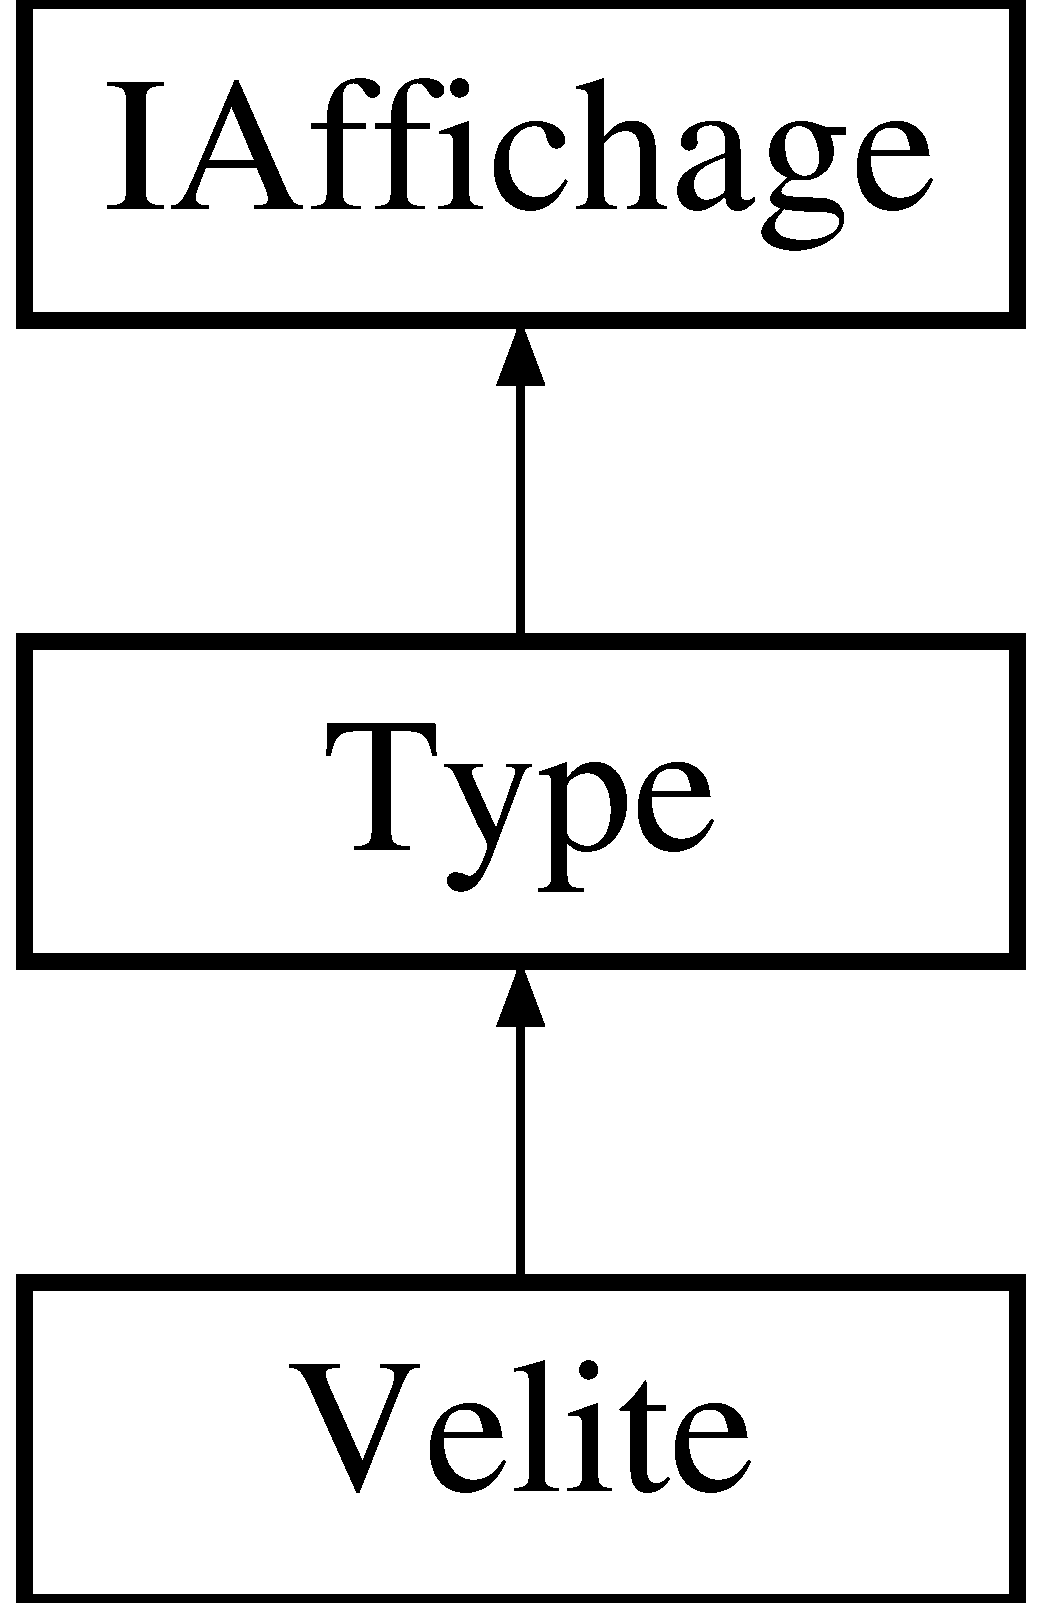
\includegraphics[height=3.000000cm]{class_velite}
\end{center}
\end{figure}
\subsection*{\-Public \-Member \-Functions}
\begin{DoxyCompactItemize}
\item 
\hyperlink{class_velite_a96681d0dbd778d6df5a677f573f9e1b3}{\-Velite} ()
\item 
int \hyperlink{class_velite_a7829a1da010495af34d315084943076e}{get\-Id} ()
\item 
void \hyperlink{class_velite_a586d8effebc0c2f29b85c49e32e1616c}{set\-Id} (int id)
\item 
string \hyperlink{class_velite_a8ee0d9986afc7c0bf2962859e39e853b}{get\-Libelle} ()
\item 
void \hyperlink{class_velite_a4fe21592a3ff3948985e81e49b52c4ad}{set\-Libelle} (string l)
\end{DoxyCompactItemize}


\subsection{\-Detailed \-Description}
\-Classe \hyperlink{class_velite}{\-Velite}, hérite de \hyperlink{class_type}{\-Type} 

\subsection{\-Constructor \& \-Destructor \-Documentation}
\hypertarget{class_velite_a96681d0dbd778d6df5a677f573f9e1b3}{\index{\-Velite@{\-Velite}!\-Velite@{\-Velite}}
\index{\-Velite@{\-Velite}!Velite@{\-Velite}}
\subsubsection[{\-Velite}]{\setlength{\rightskip}{0pt plus 5cm}{\bf \-Velite\-::\-Velite} (
\begin{DoxyParamCaption}
{}
\end{DoxyParamCaption}
)\hspace{0.3cm}{\ttfamily  \mbox{[}inline\mbox{]}}}}\label{class_velite_a96681d0dbd778d6df5a677f573f9e1b3}
\-Constructeur explicite initialisant les variables du type 

\subsection{\-Member \-Function \-Documentation}
\hypertarget{class_velite_a7829a1da010495af34d315084943076e}{\index{\-Velite@{\-Velite}!get\-Id@{get\-Id}}
\index{get\-Id@{get\-Id}!Velite@{\-Velite}}
\subsubsection[{get\-Id}]{\setlength{\rightskip}{0pt plus 5cm}int {\bf \-Velite\-::get\-Id} (
\begin{DoxyParamCaption}
{}
\end{DoxyParamCaption}
)\hspace{0.3cm}{\ttfamily  \mbox{[}inline\mbox{]}}}}\label{class_velite_a7829a1da010495af34d315084943076e}
\-Accesseur à l'identifiant du type 

\-Reimplemented from \hyperlink{class_type_aba890fe7677f58f7135ec0cfe1b7c926}{\-Type}.

\hypertarget{class_velite_a8ee0d9986afc7c0bf2962859e39e853b}{\index{\-Velite@{\-Velite}!get\-Libelle@{get\-Libelle}}
\index{get\-Libelle@{get\-Libelle}!Velite@{\-Velite}}
\subsubsection[{get\-Libelle}]{\setlength{\rightskip}{0pt plus 5cm}string {\bf \-Velite\-::get\-Libelle} (
\begin{DoxyParamCaption}
{}
\end{DoxyParamCaption}
)\hspace{0.3cm}{\ttfamily  \mbox{[}inline\mbox{]}}}}\label{class_velite_a8ee0d9986afc7c0bf2962859e39e853b}
\-Accesseur au libellé du type 

\-Reimplemented from \hyperlink{class_type_a38a529eb6a80a3d3cb801996cc9f41f0}{\-Type}.

\hypertarget{class_velite_a586d8effebc0c2f29b85c49e32e1616c}{\index{\-Velite@{\-Velite}!set\-Id@{set\-Id}}
\index{set\-Id@{set\-Id}!Velite@{\-Velite}}
\subsubsection[{set\-Id}]{\setlength{\rightskip}{0pt plus 5cm}void {\bf \-Velite\-::set\-Id} (
\begin{DoxyParamCaption}
\item[{int}]{id}
\end{DoxyParamCaption}
)\hspace{0.3cm}{\ttfamily  \mbox{[}inline\mbox{]}}}}\label{class_velite_a586d8effebc0c2f29b85c49e32e1616c}
\-Mutateur de l'identifiant du type 

\-Reimplemented from \hyperlink{class_type_ab9b8158dca9be6184557382ec98ec4f7}{\-Type}.

\hypertarget{class_velite_a4fe21592a3ff3948985e81e49b52c4ad}{\index{\-Velite@{\-Velite}!set\-Libelle@{set\-Libelle}}
\index{set\-Libelle@{set\-Libelle}!Velite@{\-Velite}}
\subsubsection[{set\-Libelle}]{\setlength{\rightskip}{0pt plus 5cm}void {\bf \-Velite\-::set\-Libelle} (
\begin{DoxyParamCaption}
\item[{string}]{l}
\end{DoxyParamCaption}
)\hspace{0.3cm}{\ttfamily  \mbox{[}inline\mbox{]}}}}\label{class_velite_a4fe21592a3ff3948985e81e49b52c4ad}
\-Mutateur du l'identifiant du type 

\-Reimplemented from \hyperlink{class_type_af475df921624fe329aaa6b19bd1ed2e1}{\-Type}.



\-The documentation for this class was generated from the following file\-:\begin{DoxyCompactItemize}
\item 
\-Projet\-P\-O\-O-\/master/\-Velite.\-cpp\end{DoxyCompactItemize}

\printindex
\end{document}
